\begin{apendicesenv}
\partapendices
\chapter{Termo de Abertura do Projeto (TAP)}
\label{ATP_app}
\section{Descrição do Projeto}

O projeto consiste no gerenciamento da medicação em instituições de longa permanência ,por meio do  desenvolvimento do dispensador automático nomeado \textit{PillWatcher}. A logo escolhida consta na Fig. \ref{fig:logo}, ilustrada abaixo:

%o qual tem aplicabilidade no armazenamento de comprimidos e auxiliar na separação e liberação da dose. Sendo assim, é possível realizar o controle de receitas com os horários definidos, bem como possíveis alterações de adição ou retirada de medicamentos através de um aplicativo.

\begin{figure}[H]
    \centering
    
\includegraphics[scale=2]{figuras/gerenciamento/pillwatcher_logo.png}
    \caption{Logomarca}
    \label{fig:logo}
\end{figure}

Além do mais, para a descrição do projeto, será utilizada a ferramenta 5W2H, um acrônimo em inglês que se refere às principais perguntas que devem ser respondidas no processo de definição do projeto. 

\begin{itemize}
\item \textit{What}?(O que) Dispensador automático de comprimidos, drágeas e capsulas.
\item \textit{Why}? (Por que) Para evitar erros de armazenamento e administração de medicamentos.
\item \textit{Where}? (Onde) Para uso em instituições de longa permanência para idosos e clinicas geriátricas.
\item \textit{When}? (Quando) O desenvolvimento será feito nos meses de agosto até dezembro.
\item \textit{Who}? (Quem) Grupo de estudantes da Faculdade do Gama de diferentes engenharias, que estão cursando a disciplina de Projeto Integrador 2.
\item \textit{How}? (Como) Será desenvolvido um dispositivo com temperatura e umidade interna monitoradas, o qual armazena medicamentos sólidos em contêineres específicos. Além do mais, possui um aplicativo onde pode-se controlar os medicamentos, registros, gerenciamento de doses diárias em horários específicos para múltiplos pacientes, assim como preparar automaticamente doses de vários pacientes em mesmo horário pré-programado. O dispositivo também permite a emissão de histórico de consumo dos medicamentos pelos pacientes.


\item \textit{How much}? (Quanto) O custo total do projeto ficou estimado em aproximadamente R\$ 13.300,00.
% Após o calculo geral dos custos adicionar aqui
\end{itemize}

\section{Propósito e Justificativa}

Percebeu-se que a forma de armazenamento da medicação em instituições de longa permanência e clinicas geriátricas não era eficiente e, em muitos casos, a forma de acondicionamento alterava a vida útil do fármaco. Além do mais, os erros podem ocorrer em qualquer etapa do processo, seja na prescrição, transcrição, distribuição, administração e monitoração das reações adversas. Entretanto, existe um número crescente de erros envolvendo a ministração de medicamentos, o que poderia ser reduzida com a utilização de um dispensador automático de medicamentos.

\section{Objetivos}

O objetivo principal do projeto é desenvolver um produto que seja capaz de gerenciar o uso de medicamentos, armazenar comprimidos, seguindo as condições térmicas e de umidade regulamentadas, e garantir que o dispositivo de uso geral dispense medicamentos na forma sólida e no horário correto pré-estabelecido, de acordo com a prescrição. 


\section{Requisitos}
Os principais requisitos de alto nível elicitados para o projeto são:

\begin{itemize}
\item Armazenar comprimidos de diferentes formatos, tamanhos e textura;
\item Facilidade e segurança no abastecimento do estoque de medicamentos;
\item Garantir um ambiente de armazenamento seguro (temperatura, umidade e sem micro-organismos);
\item Armazenar comprimidos de, no mínimo, 5 pacientes;
\item O dispensador necessita emitir sinais de alerta;
\item Assegurar que a dose medicamentosa esteja correta para um paciente específico;
\item O sistema deverá notificar os usuários em relação a doses não tomadas;
\item Regularidade no horário de ministração de medicamentos;
\item O sistema deve ter alguma forma de identificação e comprovação do paciente;
\item O dispositivo e o aplicativo deve ter interface de fácil uso;
\item Visualização do histórico de medicamentos dos pacientes;
\item Facilidade e segurança no abastecimento de medicamento;
\end{itemize}

\section{Riscos do Projeto}

\begin{table}[H]
    \centering
    \caption{Riscos e Restrições Organizacionais}
    \label{tab:tap-riscos}
    \begin{adjustbox}{max width = \textwidth}
    % \begin{adjustwidth}{-2,5cm}{}
        \begin{tabular}{|L{5cm}|c|L{4cm}|c|c|c|}
            \hline
            \rowcolor[HTML]{A8DADC}
            \textbf{ID} & \textbf{Ação} & \textbf{Ação Reativa} & \textbf{Probabilidade} & \textbf{Impacto} & \textbf{Prioridades}\\ \hline
             Desistência da disciplina  & Mitigar & Redistribuir atividades e responsabilidades & 2 & 4 & 8 \\ \hline
        
             Inexperiência da equipe  & Prevenir & Nivelar o conhecimento entre cada sub-equipe & 3 & 4 & 12 \\ \hline
             
             Alteração no escopo & Mitigar & Optar por soluções que evitem o retrabalho do que já se encontra implementado & 3 & 5 & 15 \\ \hline
             
             Dificuldade de comunicação com as clínicas geriátricas durante a pandemia & Mitigar & Buscar por artigos, protocolos e normas farmacêuticas & 4 & 3 & 12 \\ \hline
              
             Dificuldade na integração do grupo durante a pandemia & Mitigar & Realizar reuniões semanais e \textit{daily meeting} entre os sub-grupos  & 1 & 5 & 5 \\ \hline
             
             Não cumprimento de prazos & Mitigar & Acompanhar o cronograma e comparar os trabalhos realizados com o trabalho planejado & 2 & 5 & 10 \\ \hline
        \end{tabular}
    % \end{adjustwidth}
    \end{adjustbox}
\end{table}

\section{Marcos do Projeto}

Os marcos do projeto são divididos em três pontos de controle. Consequentemente, as datas principais e as respectivas atividades estão presentes na Tab.~\ref{tab:marcos}.

\begin{table}[H]
    \centering
    \caption{Marcos do Projeto}
    \label{tab:marcos}
    \begin{tabularx}{\textwidth}{|c|X|c|}
        \hline
        \rowcolor[HTML]{A8DADC}
        \textbf{Marco} & \textbf{Descrição} & \textbf{Data} \\ \hline
        Ponto de Controle 1 & Definição da problemática, e seu refinamento. Detalhamento da solução e escopo & 18/9 \\\hline
        Ponto de Controle 2 &  Modelagem, cálculos, simulação e testes da solução proposta e dos subsistemas que a compõe. & 16/10 \\ \hline
        Ponto de Controle 3 & Integração dos subsistemas e desenvolvimento de manuais para o usuário & 13/11 \\ \hline
    \end{tabularx}
\end{table}


\section{Premissas e Restrições}

\begin{itemize}
    \item O equipamento deve funcionar interligado à rede elétrica;
    \item O equipamento possuirá um sistema de alimentação secundária (bateria de reserva), que somente em casos emergenciais será acionado;
    \item O usuário deve ter facilidade no abastecimento de medicamentos;
    \item O usuário deve ter facilidade em retirar o recipiente do dispensador;
    \item O usuário deve ter segurança em identificar o recipiente para cada paciente. 
    \item O gerenciamento do dispensador deve ser remoto;
    \item O dispositivo deve ser fixo;
    \item Em hipótese alguma o equipamento deve operar em paralelo com o sistema de alimentação principal;
    \item Não são aceitos medicamentos líquidos, pastosos, injetáveis, meias pílulas, gomas, pílulas em pó, pegajosas ou dissolvíveis.
    \item O usuário deve conectar o dispositivo na rede mundial de computadores;
    \item O dispositivo não deverá ser submetido a movimentos bruscos, visto que o mesmo estará com os medicamentos armazenados e dispositivos sensíveis.
\end{itemize}

\section{Stakeholders}
O projeto vigente possui quatro \textit{stakeholders} identificados: a equipe do projeto, os professores da disciplina, farmacêuticos e as instituições de longa permanência.

\begin{itemize}
\item \textbf{Equipe de Projeto}:

A equipe é formada por 14 alunos da Universidade de Brasília (UnB) do Campus Gama (FGA), de cursos de Engenharia Aeroespacial, Automotiva, Eletrônica e Software que estão cursando a disciplina Projeto Integrador 2. A equipe tem como responsabilidade  comparecer às reuniões, realizar o estudo teórico e de viabilidade do projeto, fornecer ideias de soluções, documentar os passos do projeto e investir tempo e dedicação. Consequentemente, as expectativas da equipe encontram-se no sucesso do projeto, assim como propor uma possível documentação para patentear.

\item \textbf{Professores da disciplina Projeto Integrador 2}:

O principal papel dos professores em relação ao projeto vigente é fornecer conhecimento teórico e prático, aliados com suas experiências nas engenharias do campus. Além de avaliar e monitorar o desenvolvimento do projeto durante a disciplina. Dessa forma, os professores tem como expectativa o sucesso do projeto e que os alunos obtenham conhecimentos específicos sobre o desenvolvimento de projeto, assim como que tenham uma noção de integração entre as engenharias durante a graduação.
\item \textbf{Farmacêuticos}:

A principal responsabilidade dos farmacêuticos é fornecer informações essenciais para o grupo definir os requisitos gerais do produto. Assim, a expectativa desse \textit{stakeholder} é garantir que o dispensador siga as normas vigentes para fármacos.

\item \textbf{Instituições de Longa Permanência para Idosos}:

É responsabilidade das clínicas geriátricas fornecer informações essenciais para definir os requisitos gerais do produto necessários para atender suas expectativas, além de fornecer o \textit{feedback} relevante para implementar melhorias.  A principal expectativa se resume em facilitar o armazenamento e a ministração de medicamentos sólidos.
\end{itemize}



\chapter{Estrutura Analítica do Projeto}
\label{EAP_app}
\section{Estrutura Analítica por Ponto de Controle}

\begin{figure}[H]
    \centering
    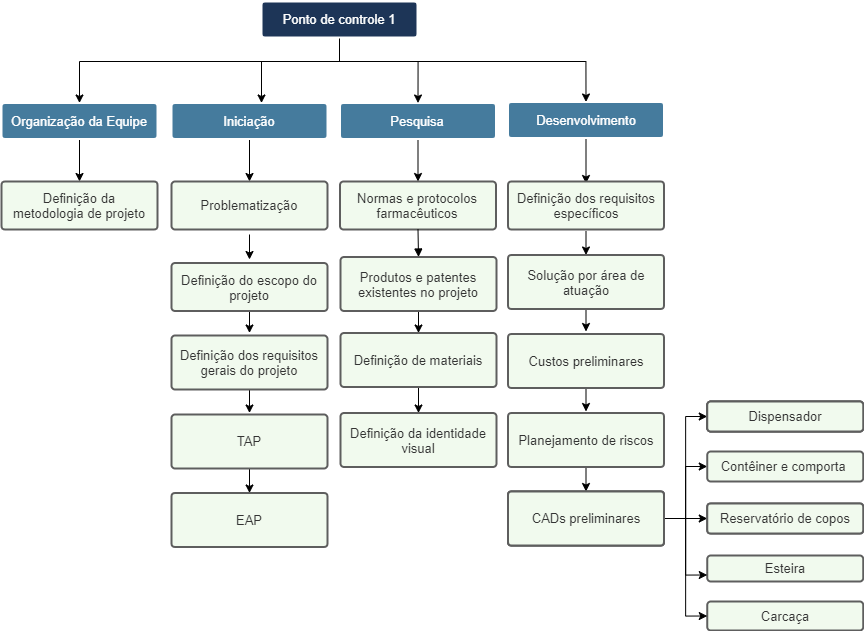
\includegraphics[width=\textwidth]{figuras/gerenciamento/eap_pc1.png}
    \caption{Estrutura Analítica do Projeto PillWatcher - Ponto de Controle 1 }
    \label{fig:eap_pc1}
\end{figure}

\begin{landscape}
\begin{figure}[H]
    \centering
    \vspace{1cm}
    \hspace{-1cm}
    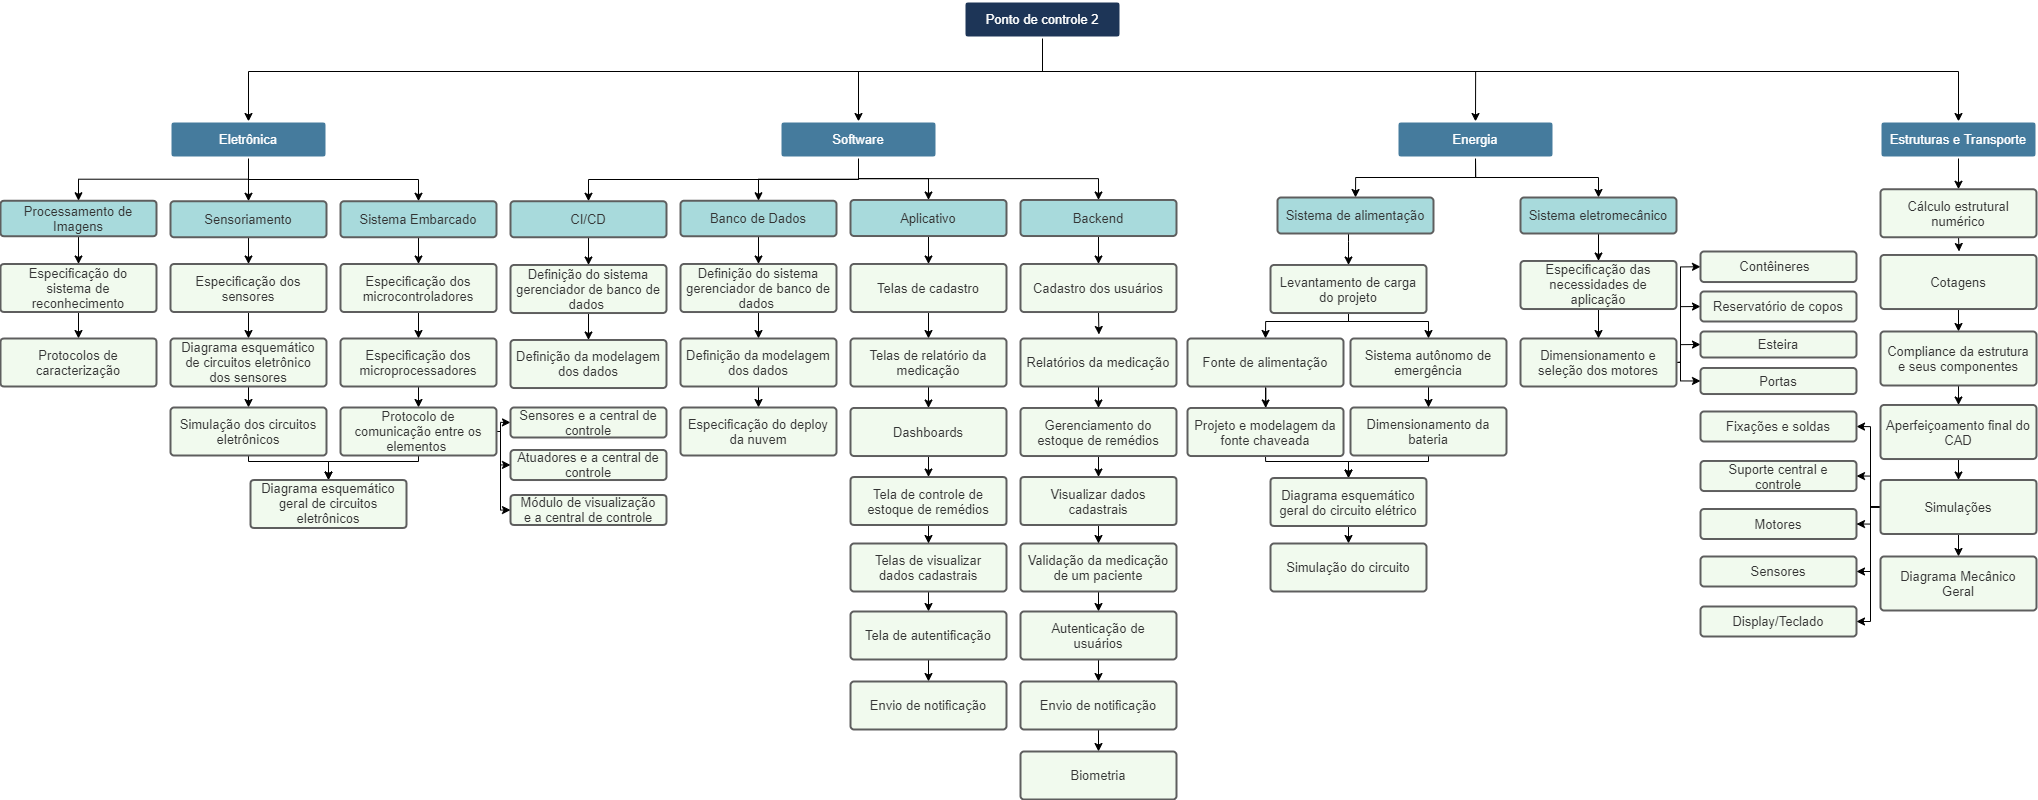
\includegraphics[scale=0.3]{figuras/gerenciamento/eap_pc2.png}
    \caption{Estrutura Analítica do Projeto PillWatcher - Ponto de Controle 2 }
    \vspace{-5pt}
    \label{fig:eap_pc2}
\end{figure}
\end{landscape}

\begin{figure}[H]
    \centering
    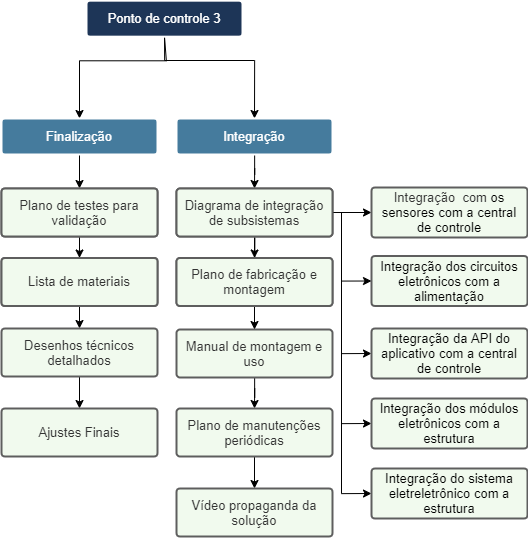
\includegraphics[width=0.7\textwidth]{figuras/gerenciamento/eap_pc3.png}
    \caption{Estrutura Analítica do Projeto PillWatcher - Ponto de Controle 3 }
    \label{fig:eap_pc3}
\end{figure}

\begin{landscape}
\section{Estrutura Analítica Geral}
\begin{figure}[!htb]
    \centering
    \vspace{2cm}
    \hspace{-2cm}
    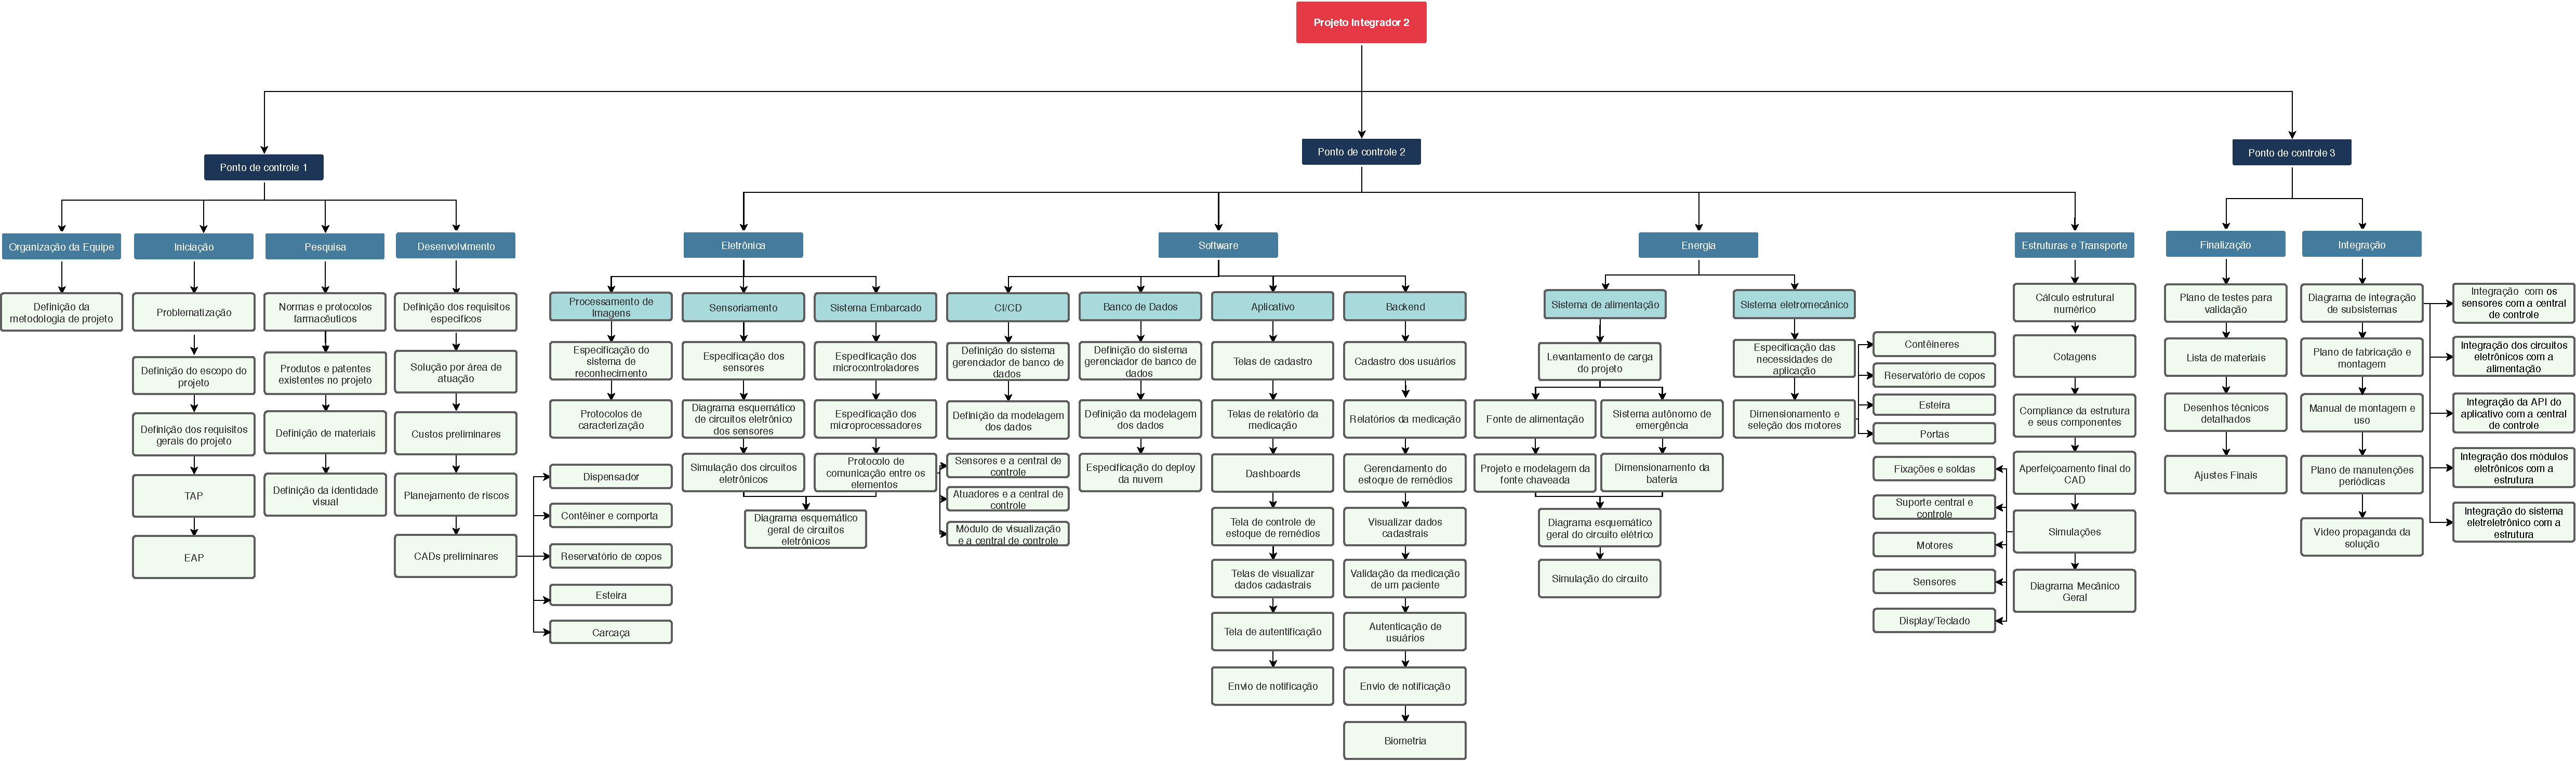
\includegraphics[width=1.55\textwidth, height=2\textheight,keepaspectratio]{figuras/gerenciamento/eap_geral.pdf}
    \vspace{-5pt}
    \caption{Estrutura Analítica do Projeto PillWatcher}
\end{figure}
\end{landscape}
%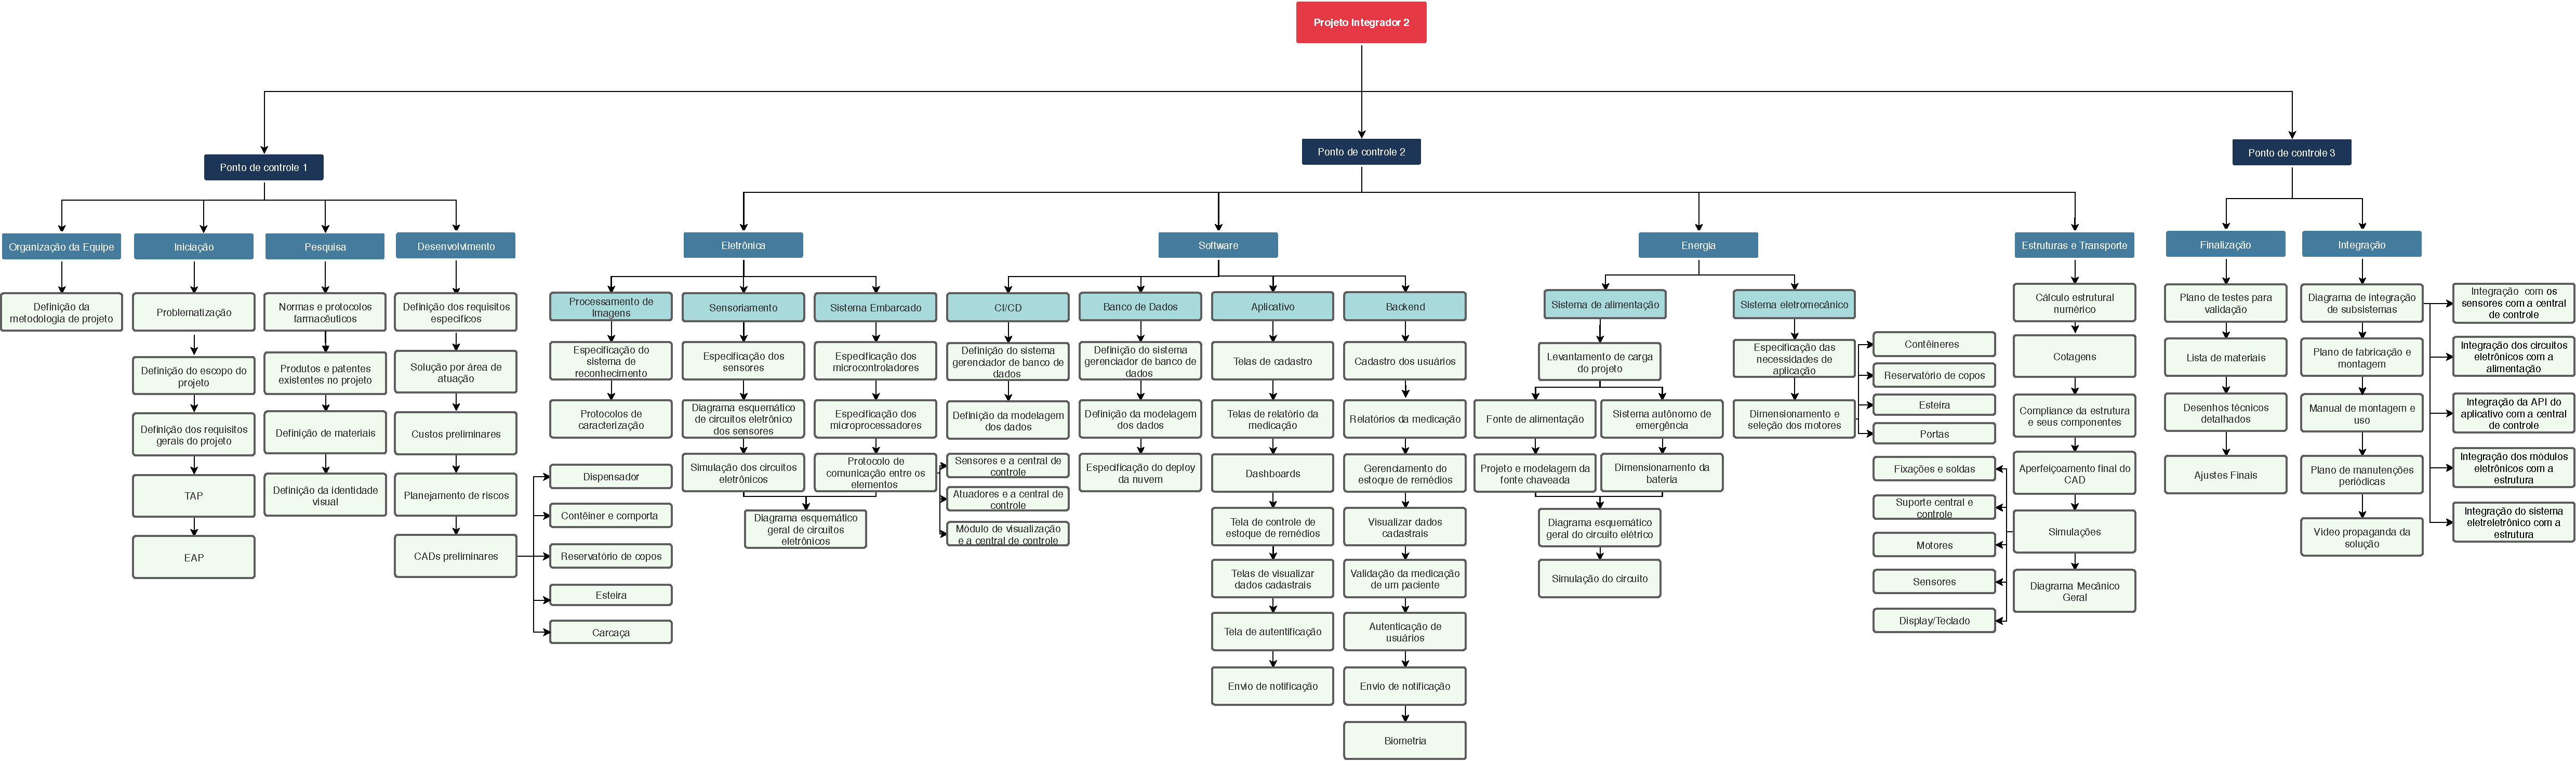
\includepdf[scale=0.73,angle=90,pages=1,pagecommand=\label{EAp}, offset=1cm -1.5cm]{figuras/EAP.pdf}

\chapter{Lista É/ Não É}
\label{Lista_app}

\begin{table}[H]
    \centering
    \caption{Lista É/Não é}
    \label{tab:lista_e_n_e}
    \begin{tabularx}{\textwidth}{|X|X|}
        \hline
        \rowcolor[HTML]{A8DADC}
        \multicolumn{1}{|X}{\textbf{É}} & \multicolumn{1}{|X|}{\textbf{Não é}} \\ 
        \hline
        1.1 É um sistema automático & 1.2 Não é um sistema autônomo \\ 
        \hline
        2.1 É um dispensador de medicamentos sólidos (comprimidos, drágeas e capsulas) & 2.2 Não é um dispensador de medicamentos líquidos, injetáveis ou pastosos \\ 
        \hline
        3.1 A quantidade de contêineres é pré-definida & 3.2 A quantidade de contêineres não é variável\\ 
        \hline
        4.1 Os contêineres recebem separadamente cada medicamento & 4.2 Os contêineres não armazenam doses de diferentes medicamentos \\
        \hline
        5.1 É um dispositivo que funciona interligado à rede elétrica & 5.2 Não é um dispositivo que deve funcionar desconectado da rede, salvo em falha da fonte primária \\ 
        \hline
        6.1 Para uso coletivo & 6.2 Para uso individual\\ 
        \hline
        7.1 Controlado via aplicativo & 7.2 Controlado manualmente via dispensador\\ 
        \hline
        8.1 Responsável por verificar se a medicação foi corretamente armazenada e separada em doses & 8.2 Responsável por ministrar a medicação\\ 
        \hline
        9.1 É um dispositivo fixo & 9.2 Não é um dispositivo transportável \\ 
        \hline
    \end{tabularx}
\end{table}


\chapter{Cronograma}\label{roadmap}

\vspace{-1.6cm}
\begin{figure}[H]
    \centering
    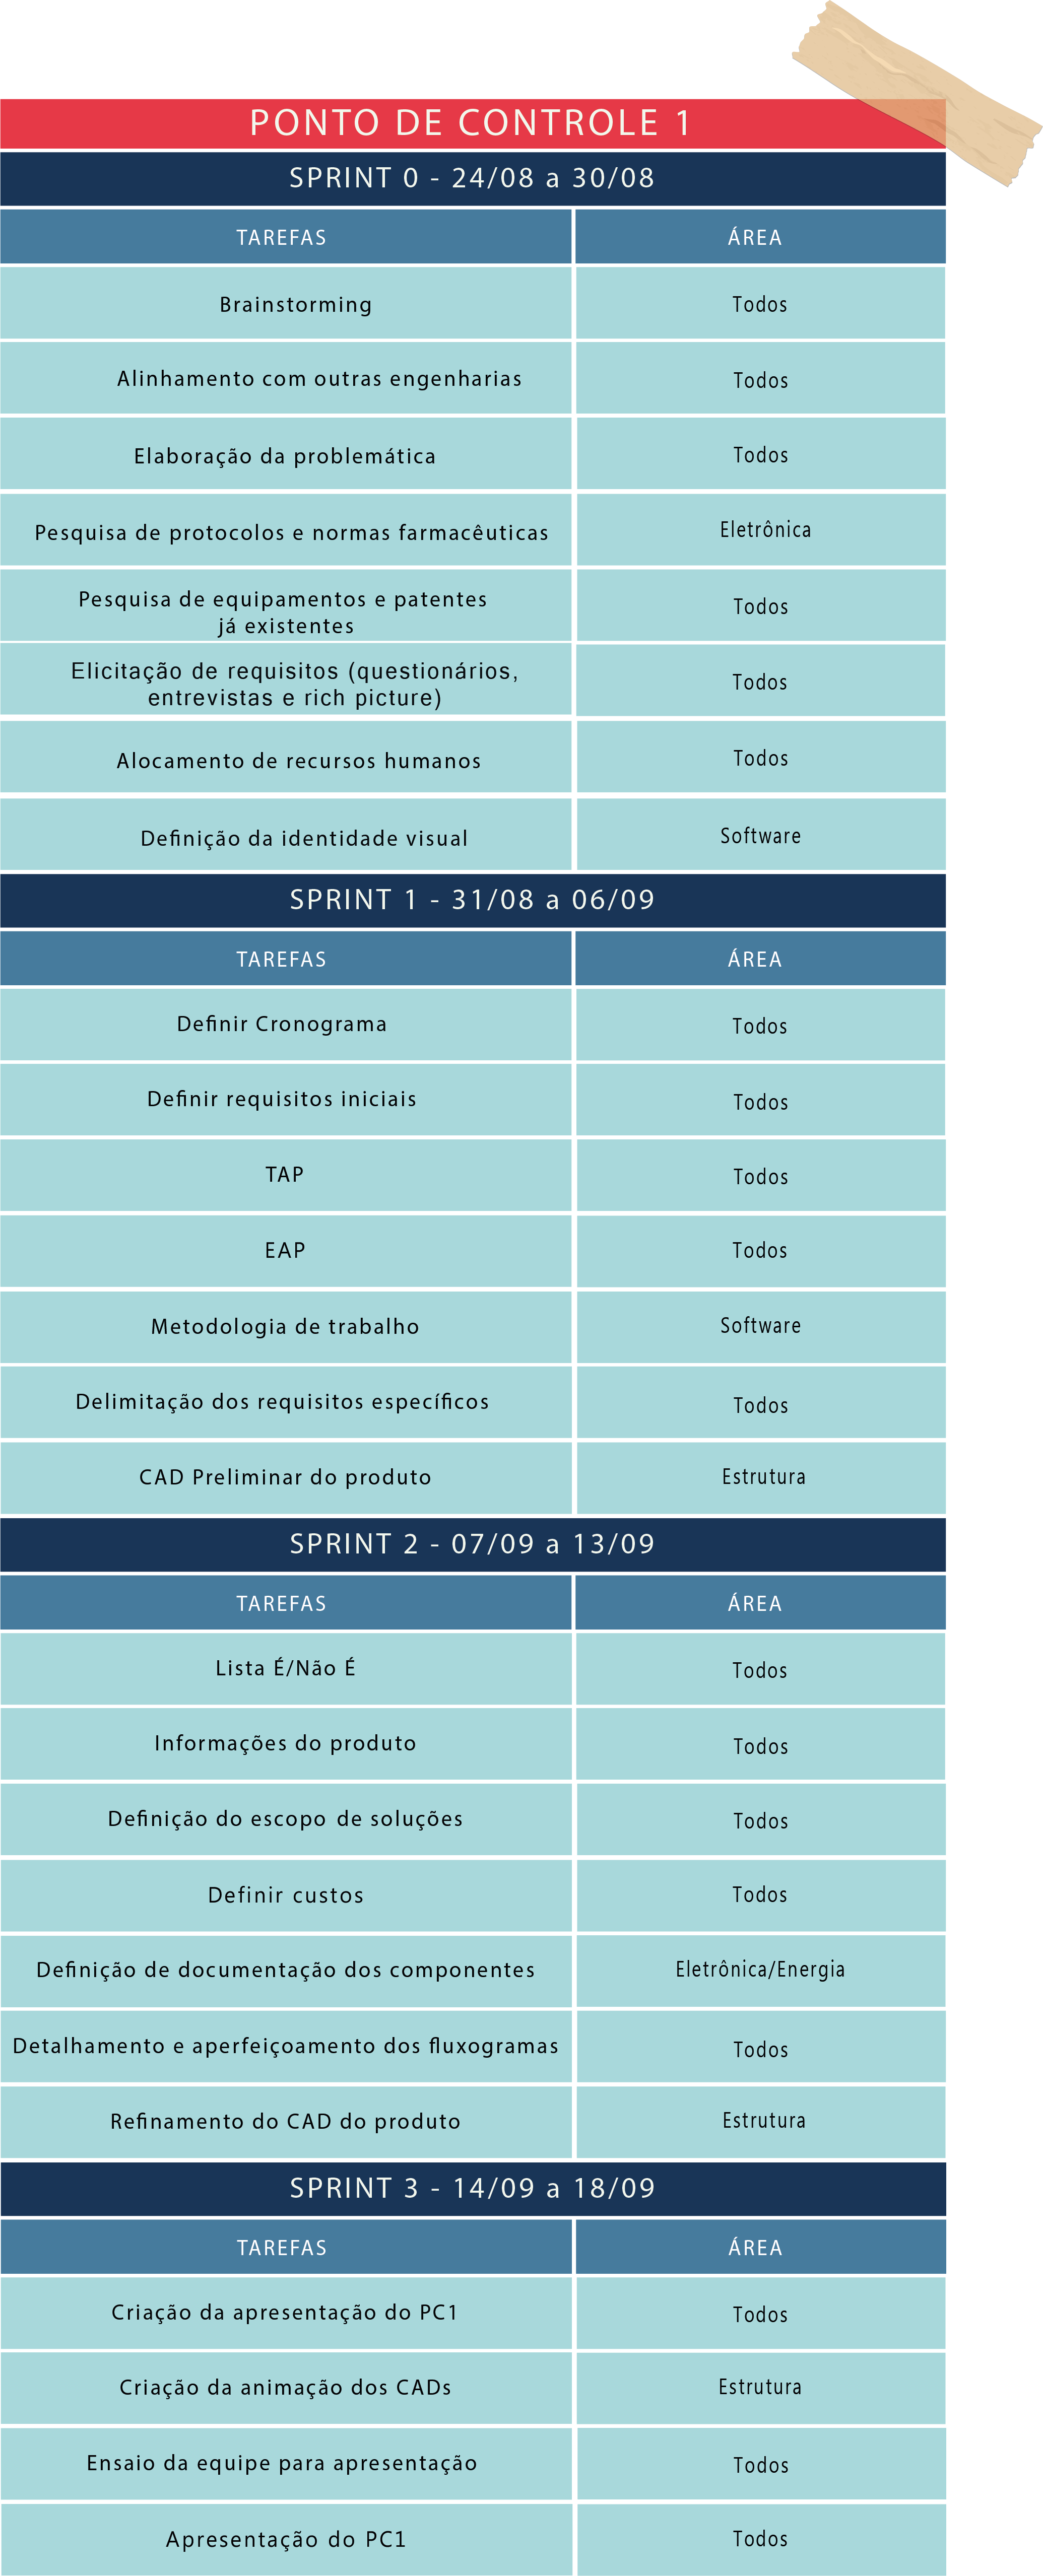
\includegraphics[width=0.5\textwidth]{figuras/gerenciamento/sprint-pc1.png}
    \caption{Planejamento Ponto de Controle 1}
    \label{fig:Sprint_pc1}
\end{figure}

\begin{figure}[H]
    \centering
    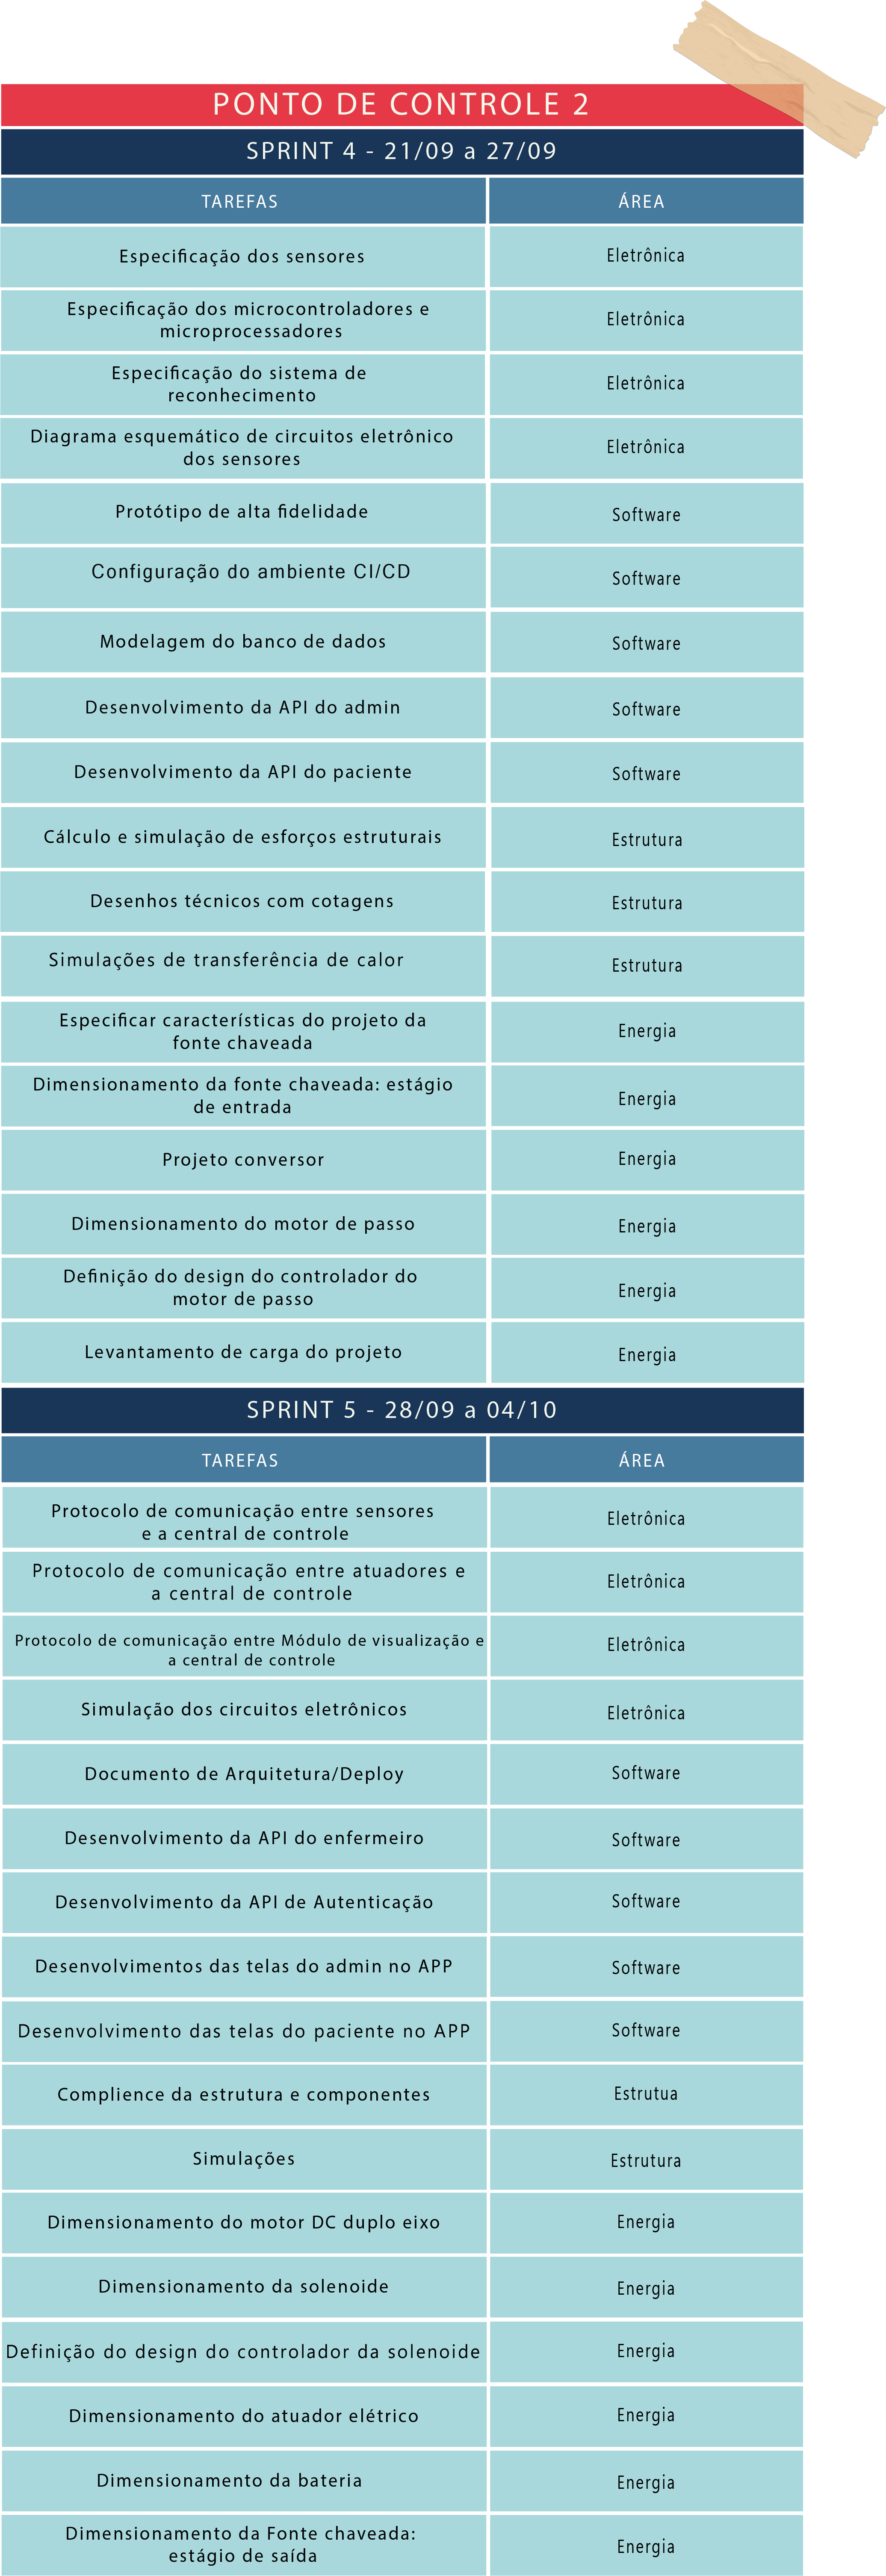
\includegraphics[width=0.5\textwidth]{figuras/gerenciamento/sprint-pc2-1.png}
    \caption{Planejamento Ponto de Controle 2}
    \label{fig:Sprint_pc2}
\end{figure}

\begin{figure}[H]
    \centering
    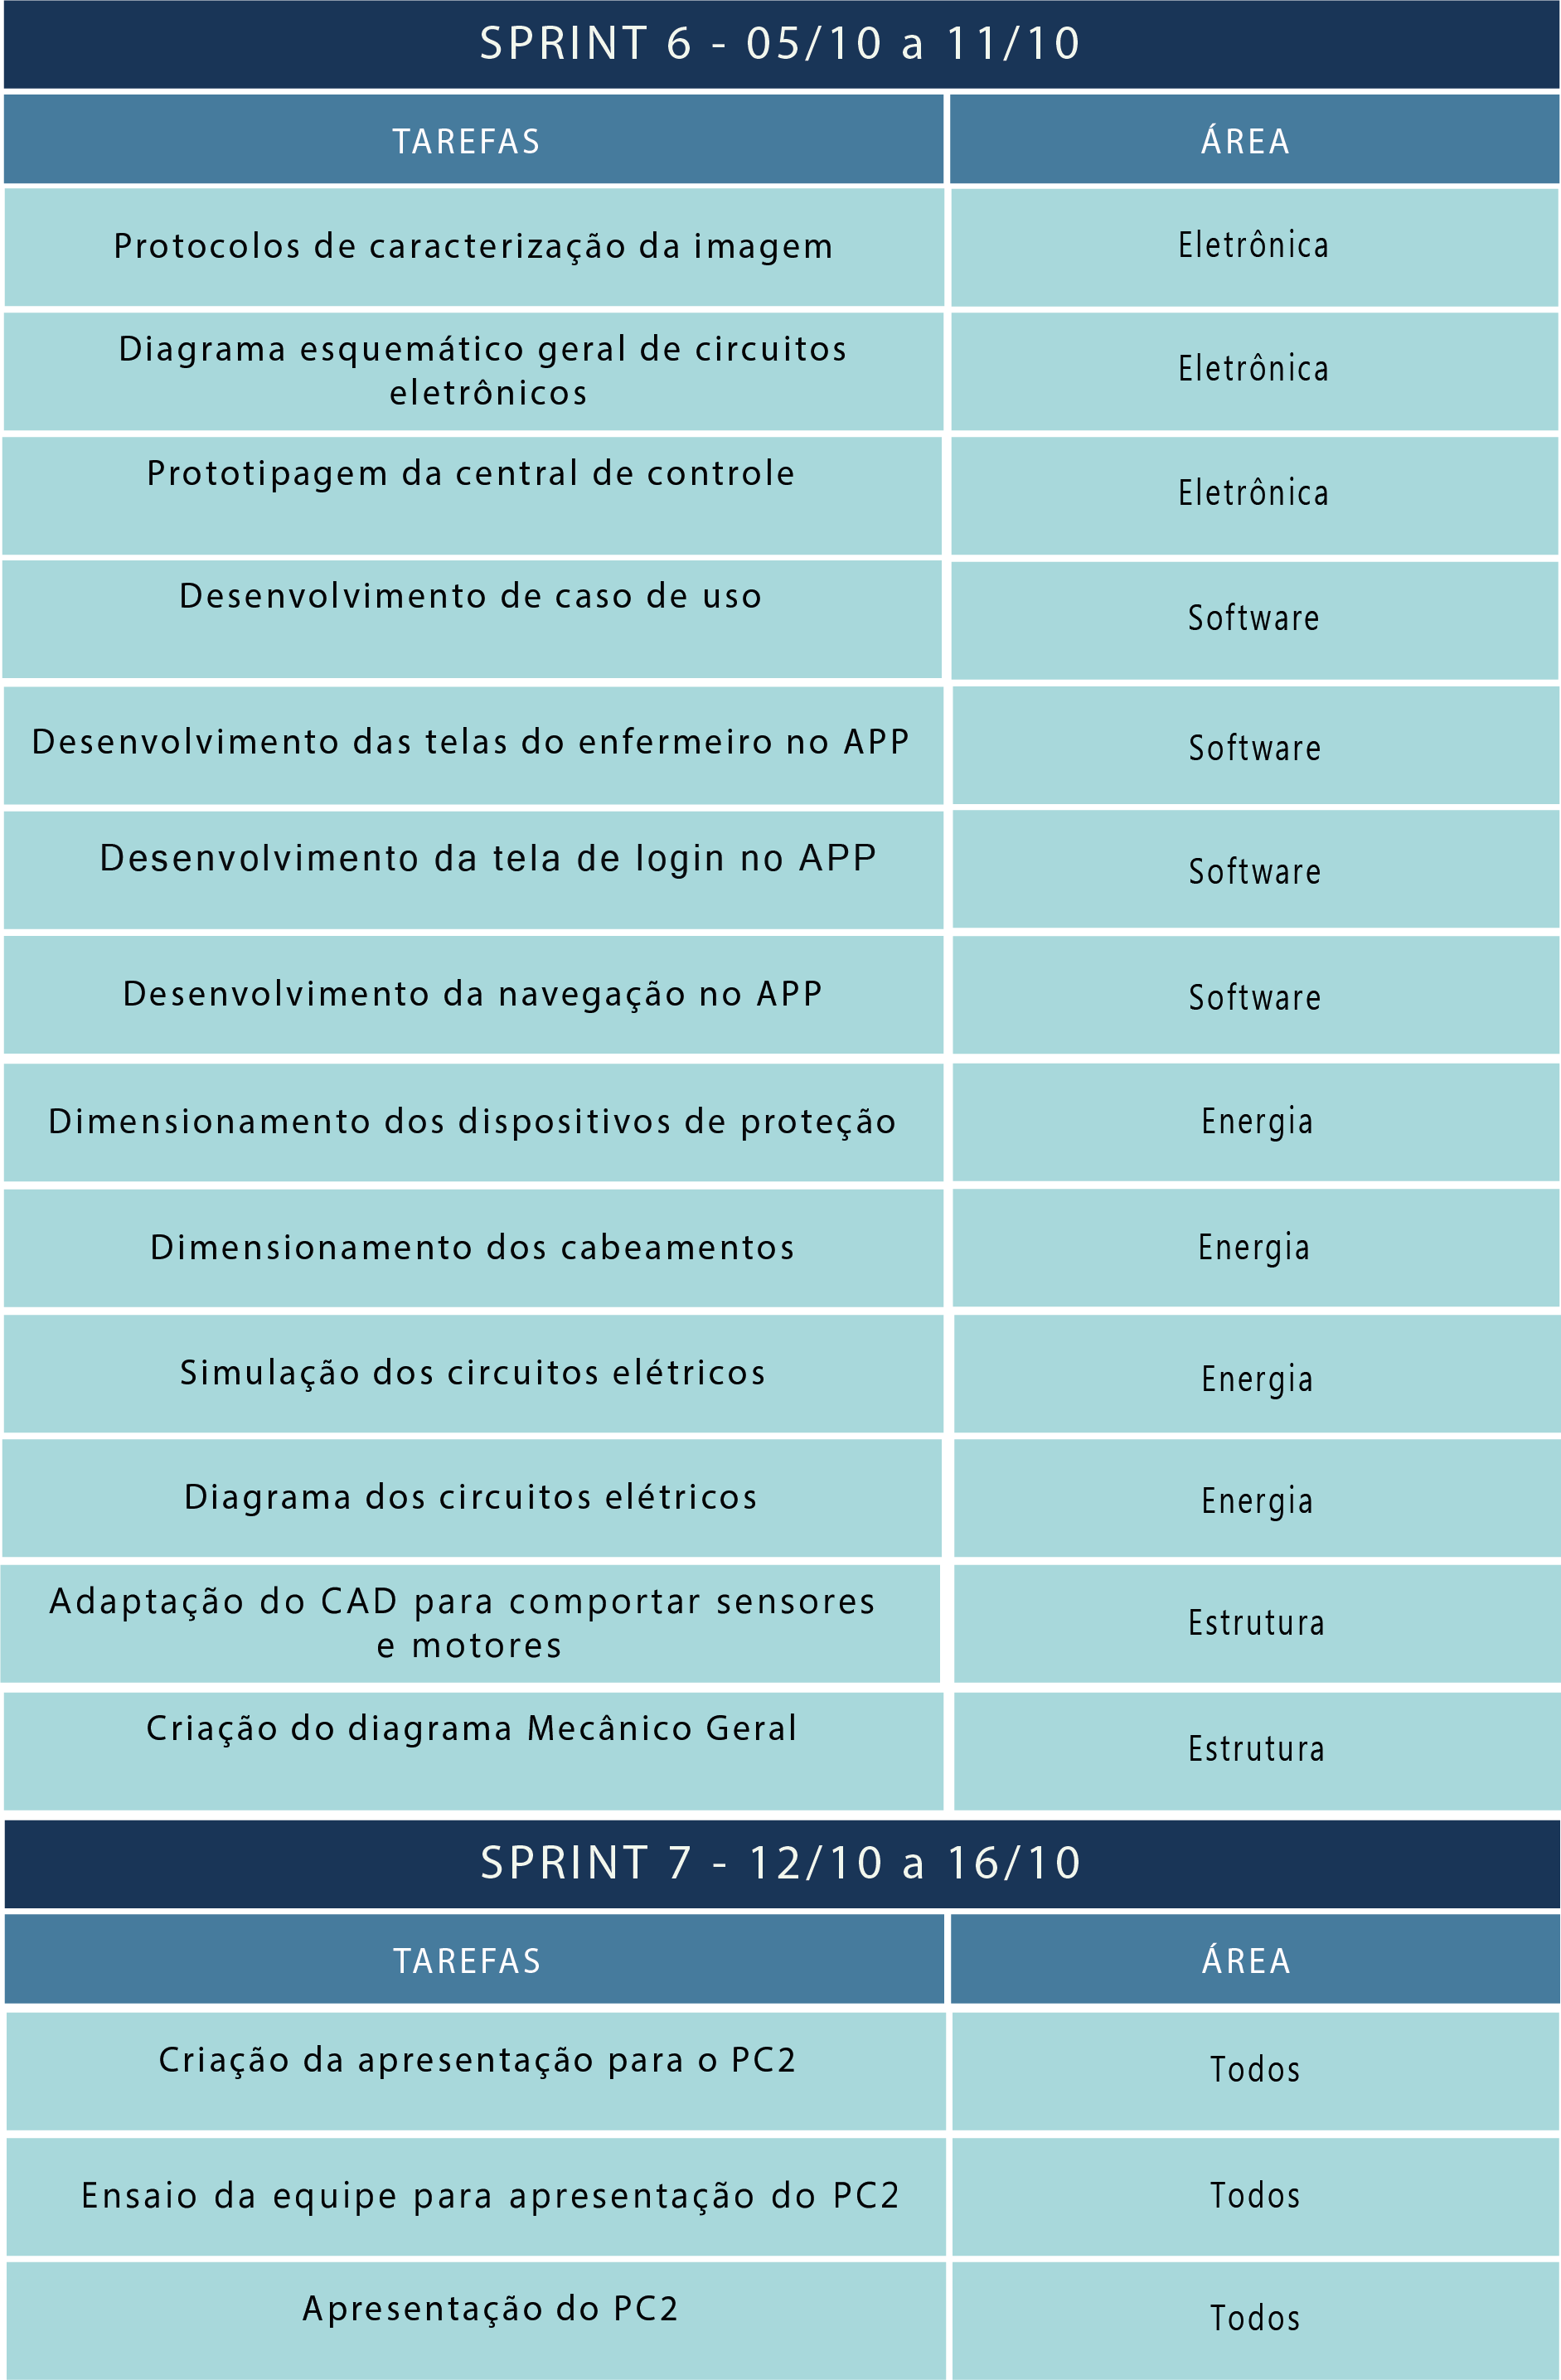
\includegraphics[width=0.5\textwidth]{figuras/gerenciamento/sprint-pc2-2.png}
    \caption{Planejamento Ponto de Controle 2}
    \label{fig:Sprint_pc2_1}
\end{figure}

\begin{figure}[H]
    \centering
    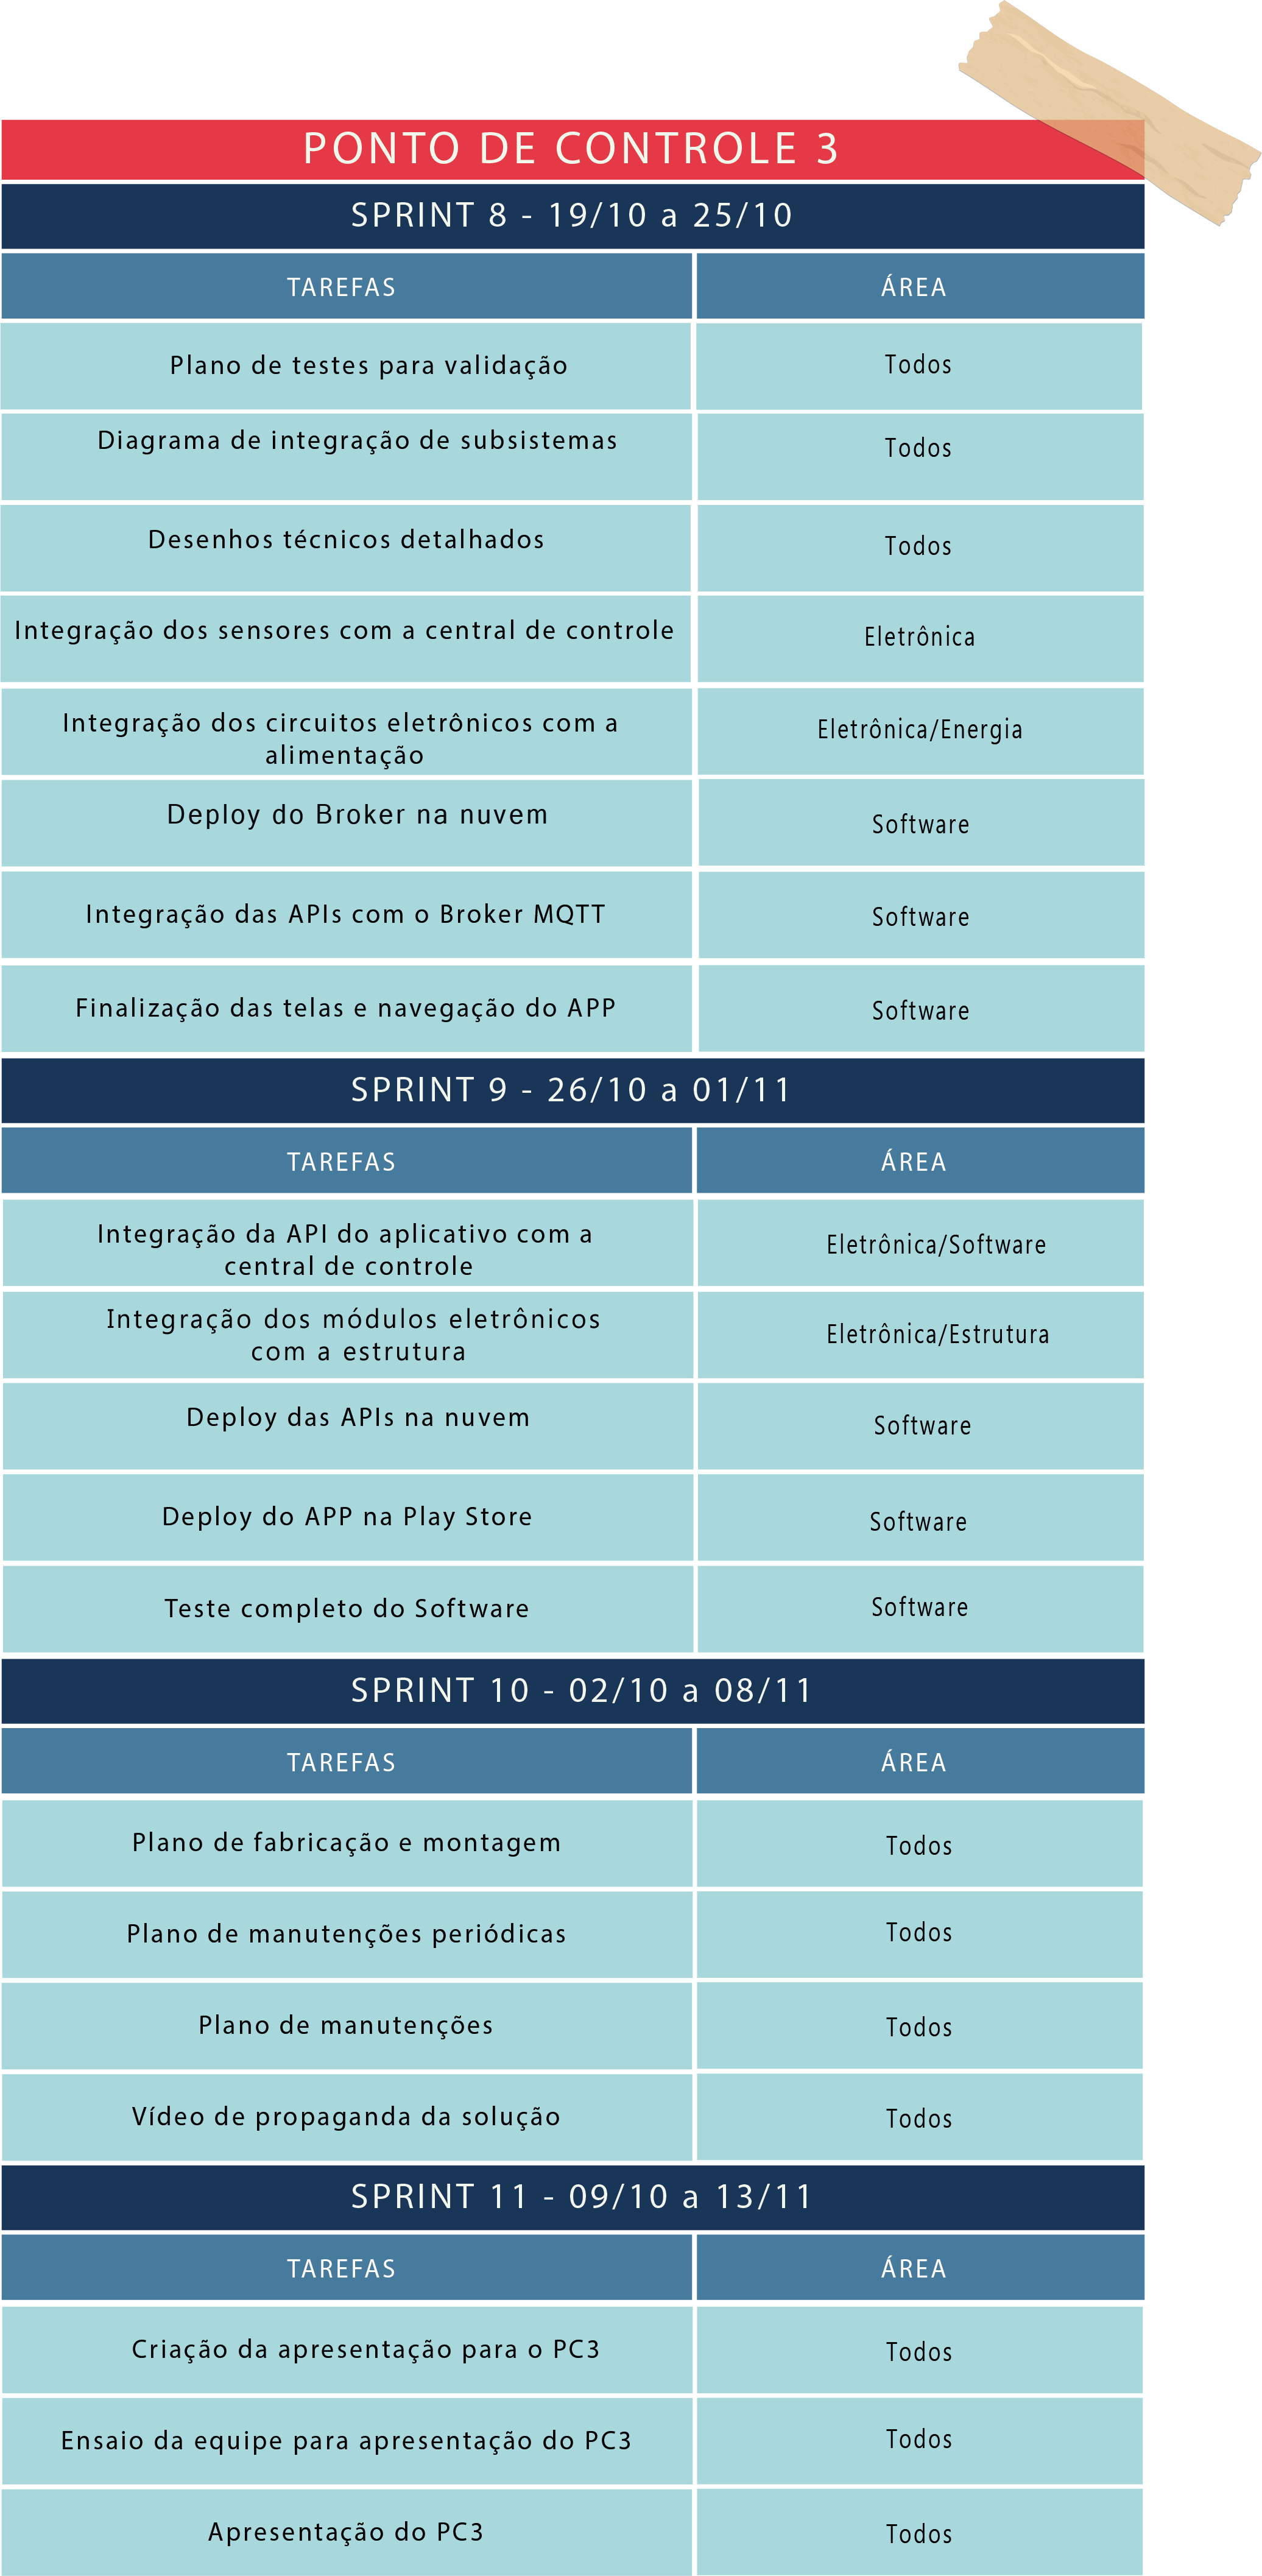
\includegraphics[width=0.5\textwidth]{figuras/gerenciamento/sprint-pc3.png}
    \caption{Planejamento Ponto de Controle 3}
    \label{fig:Sprint_pc3}
\end{figure}

% CADs Preliminares
\chapter{Desenhos Técnicos}\label{cad_preliminar}

\vspace{3cm}

\begin{figure}[H]
    \centering
    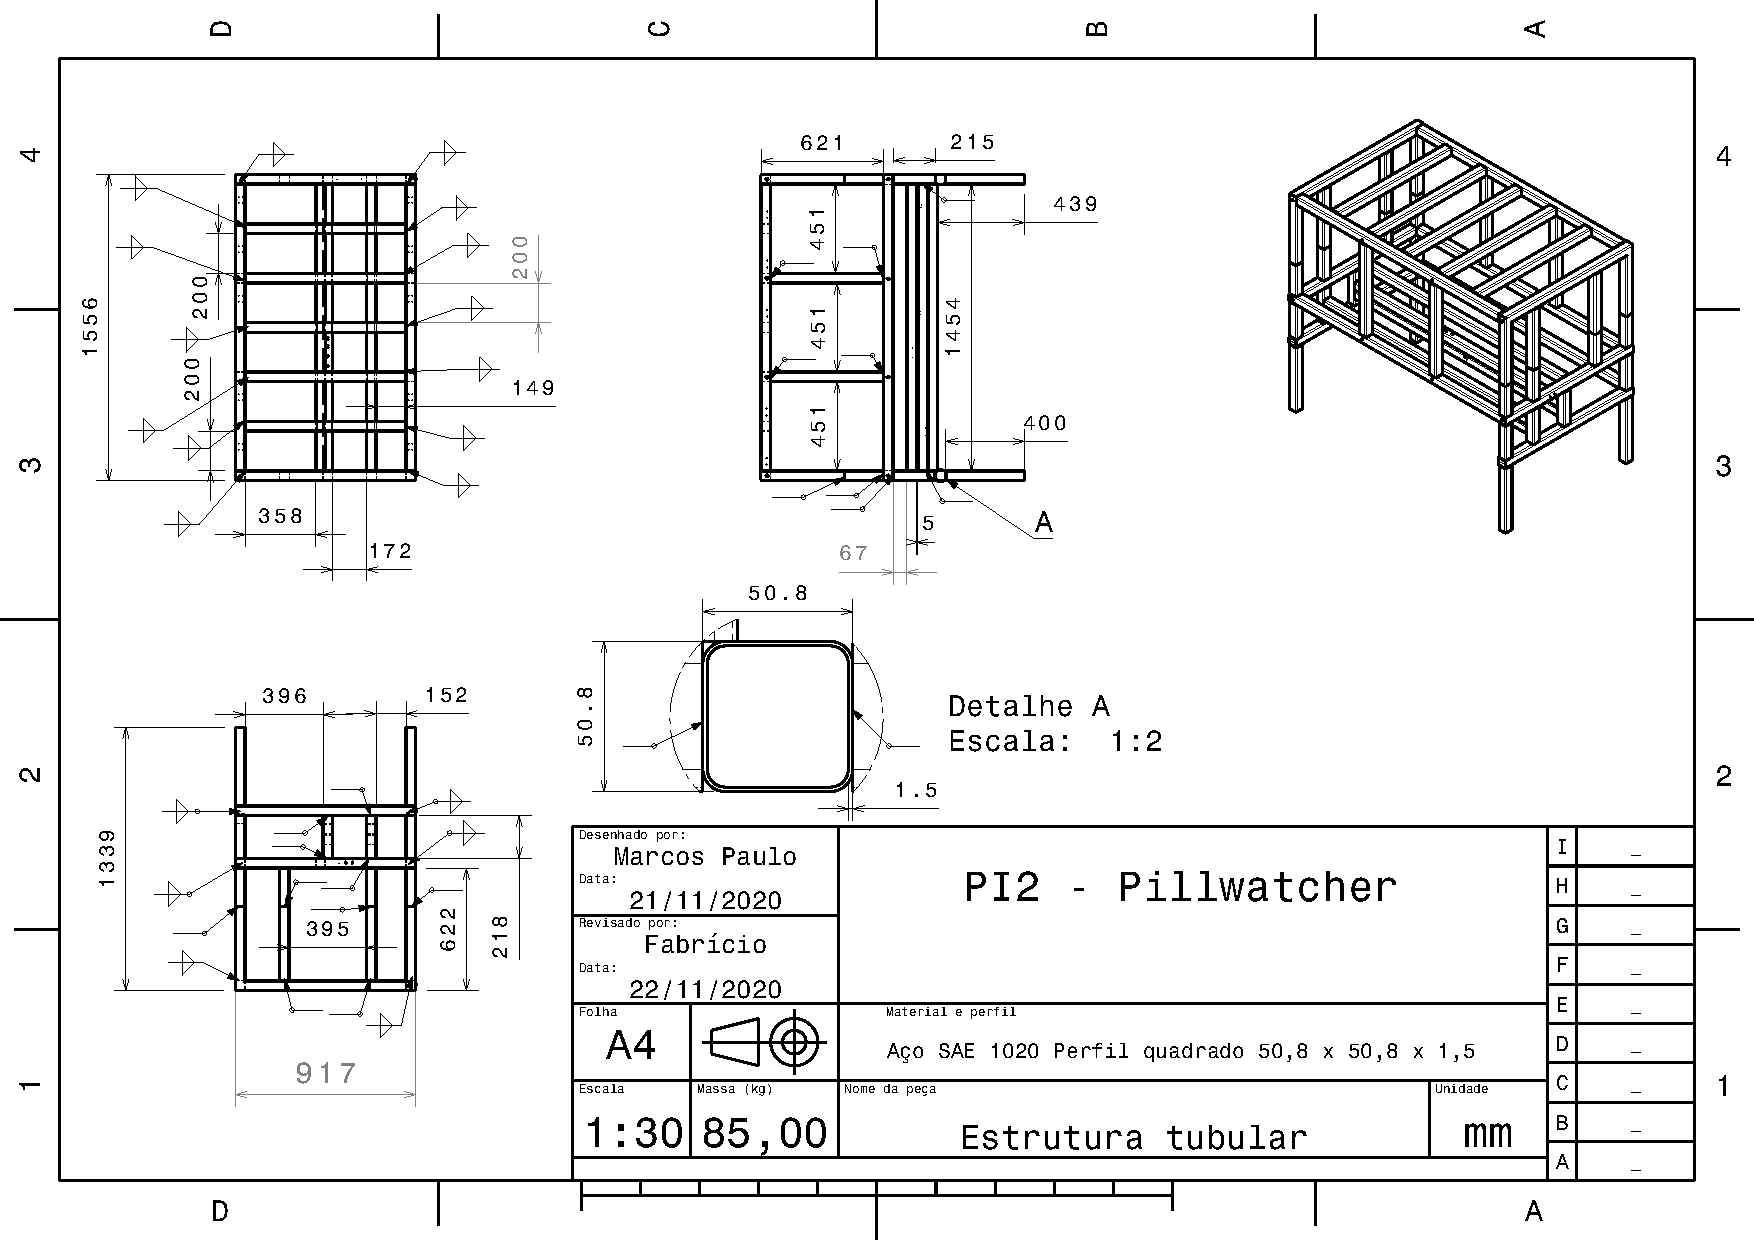
\includegraphics[width=1\textwidth]{figuras/estrutura/Desenhos/Estrutura_Tubular_V2.pdf}
    \caption{Desenho técnico da Estrutura Tubular, com indicações de solda (\ref{retorno_tubos_perfilquadrado})}
    \label{fig:estruturatubular}
\end{figure}

\begin{figure}[H]
    \centering
    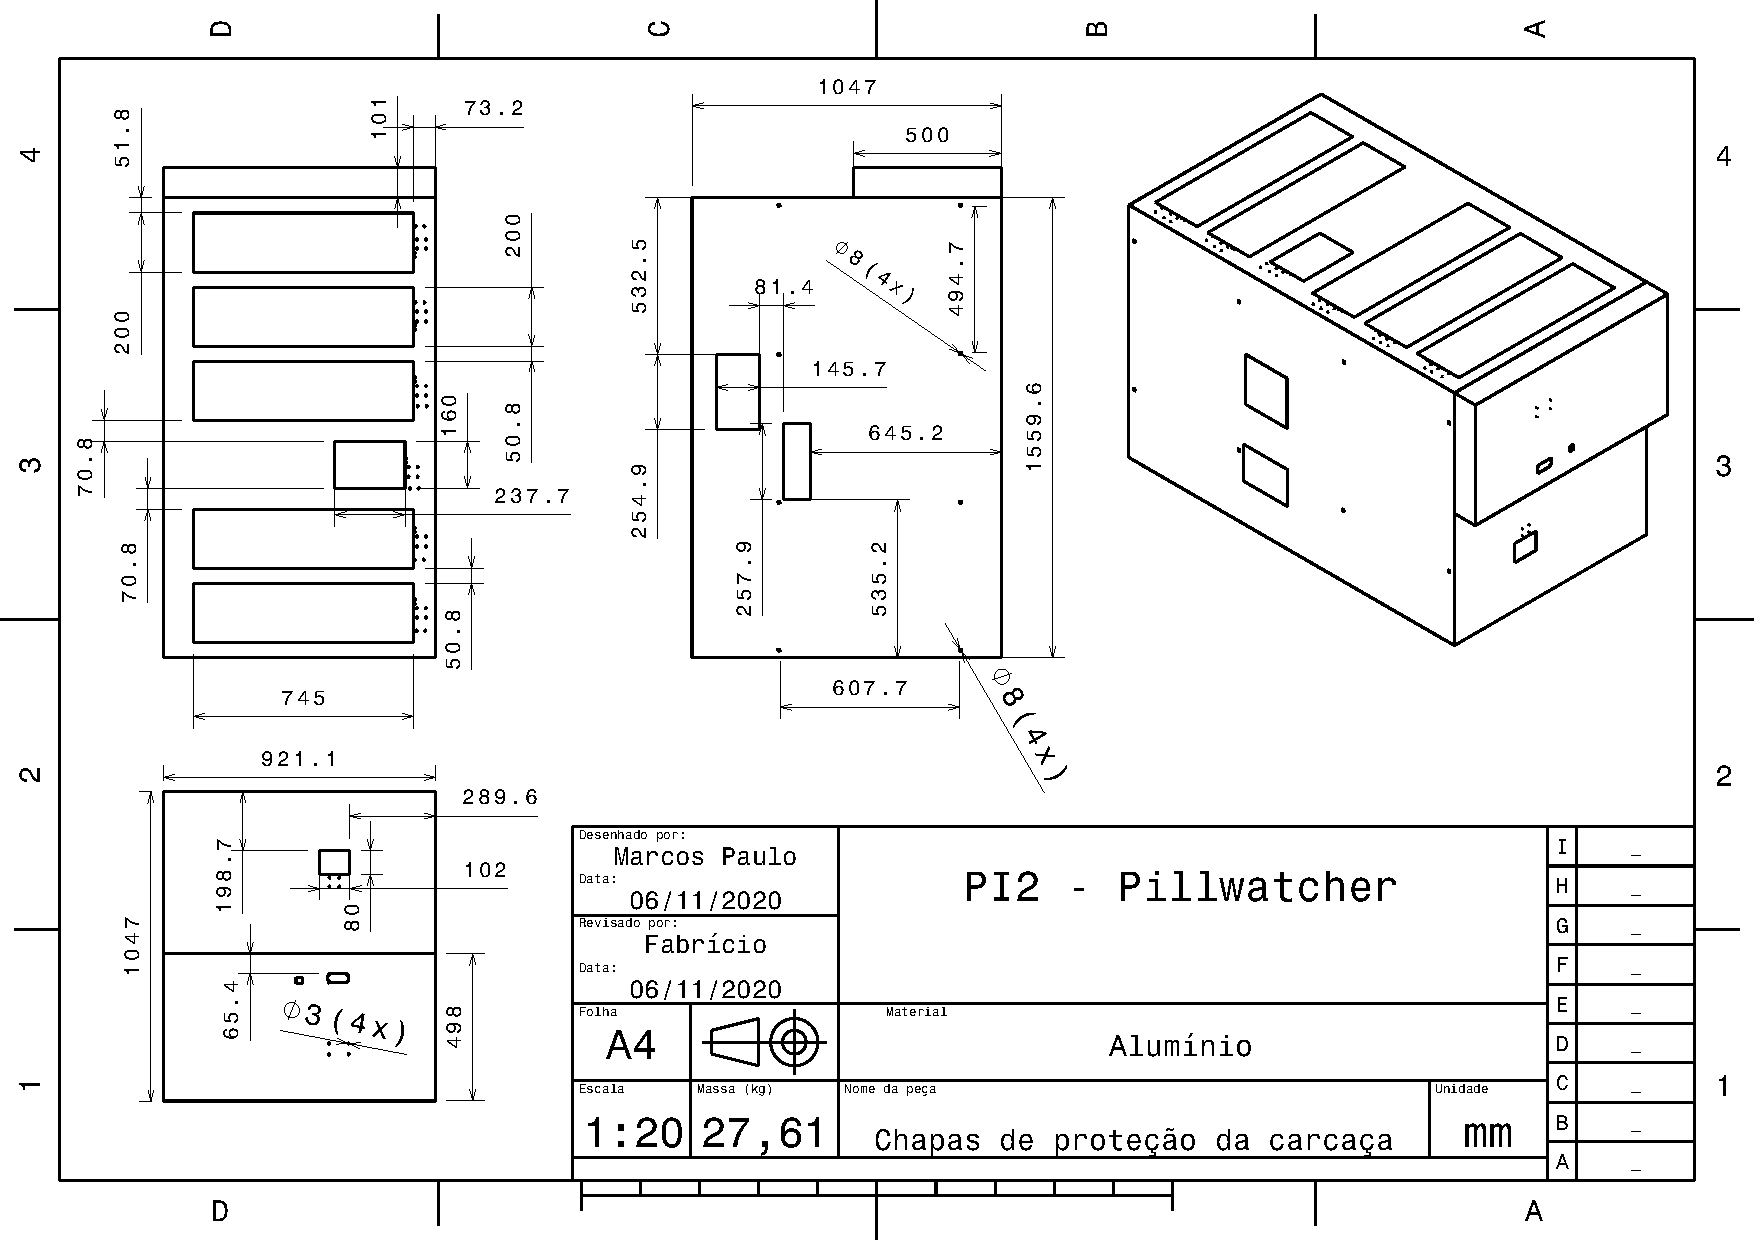
\includegraphics[width=0.9\textwidth]{figuras/estrutura/Desenhos/Chapas_Exterior.pdf}
    \caption{Desenho técnico das Chapas da Carcaça (\ref{retorno_chapas})}
    \label{fig:chapasexterior}
\end{figure}

\begin{figure}[H]
    \centering
    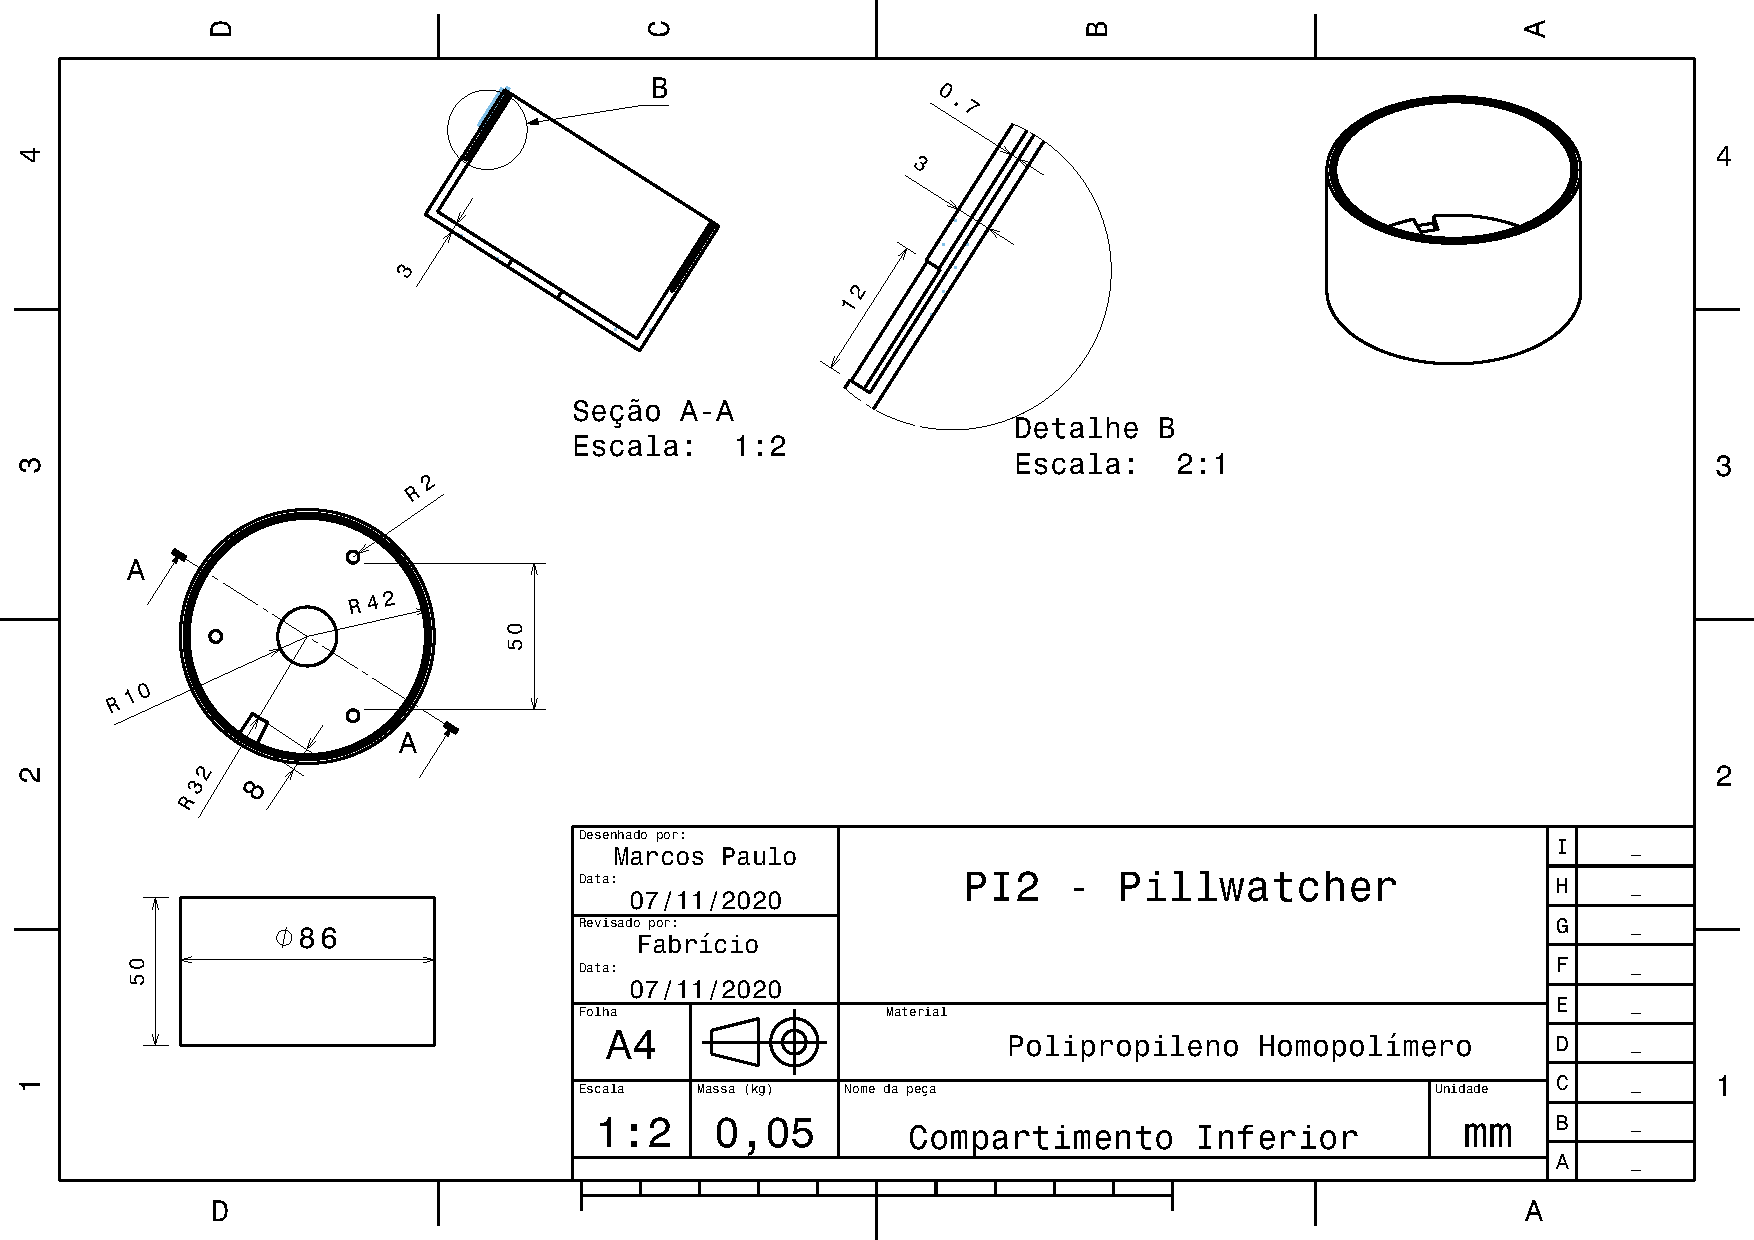
\includegraphics[width=0.9\textwidth]{figuras/estrutura/Desenhos/Compartimento_Inferior.pdf}
    \caption{Desenho técnico do Compartimento Inferior do Contêiner (\ref{retorno_compartimentoinferior})}
    \label{fig:compartimentoinferior}
\end{figure}

\begin{figure}[H]
    \centering
    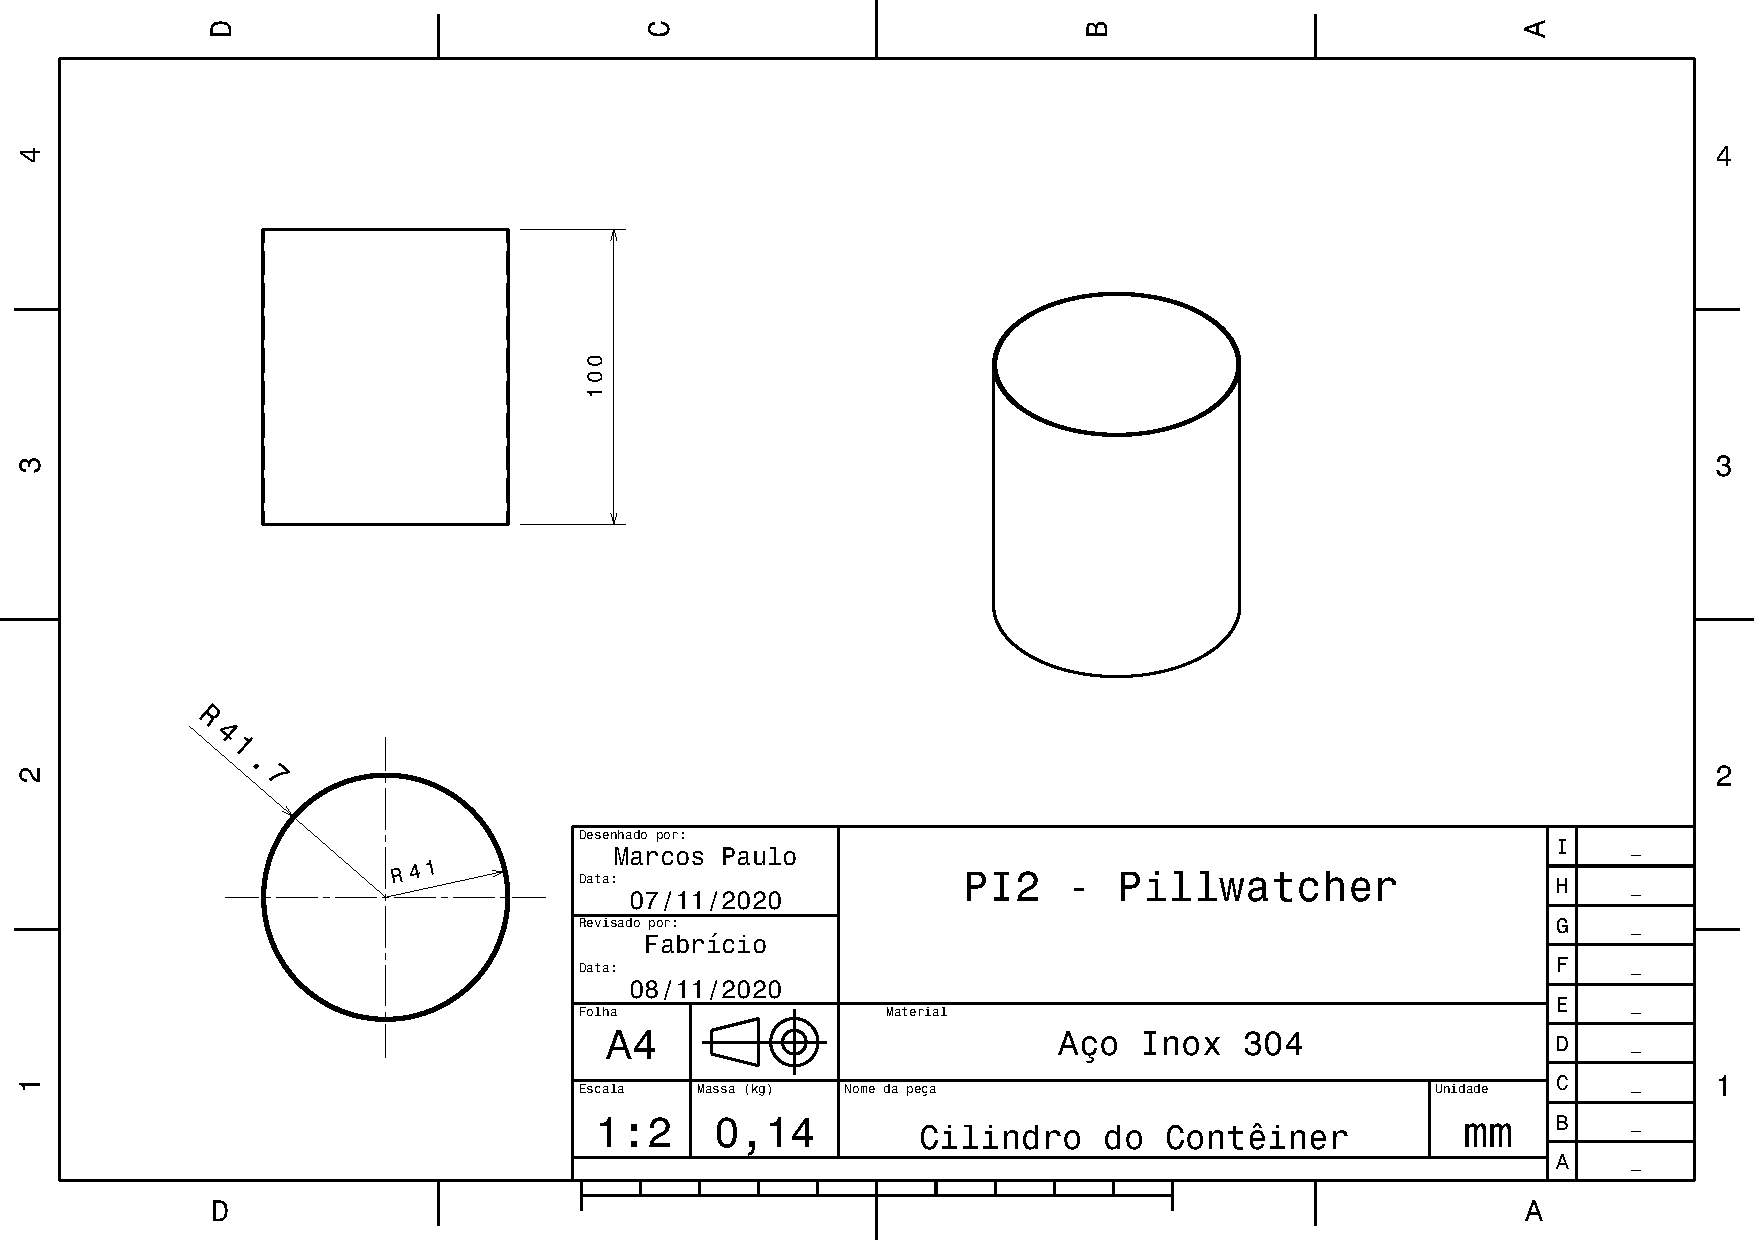
\includegraphics[width=0.9\textwidth]{figuras/estrutura/Desenhos/Cilindro.pdf}
    \caption{Desenho técnico do cilindro do contêiner (\ref{retorno_cilindro})}
    \label{fig:cilindro}
\end{figure}

\begin{figure}[H]
    \centering
    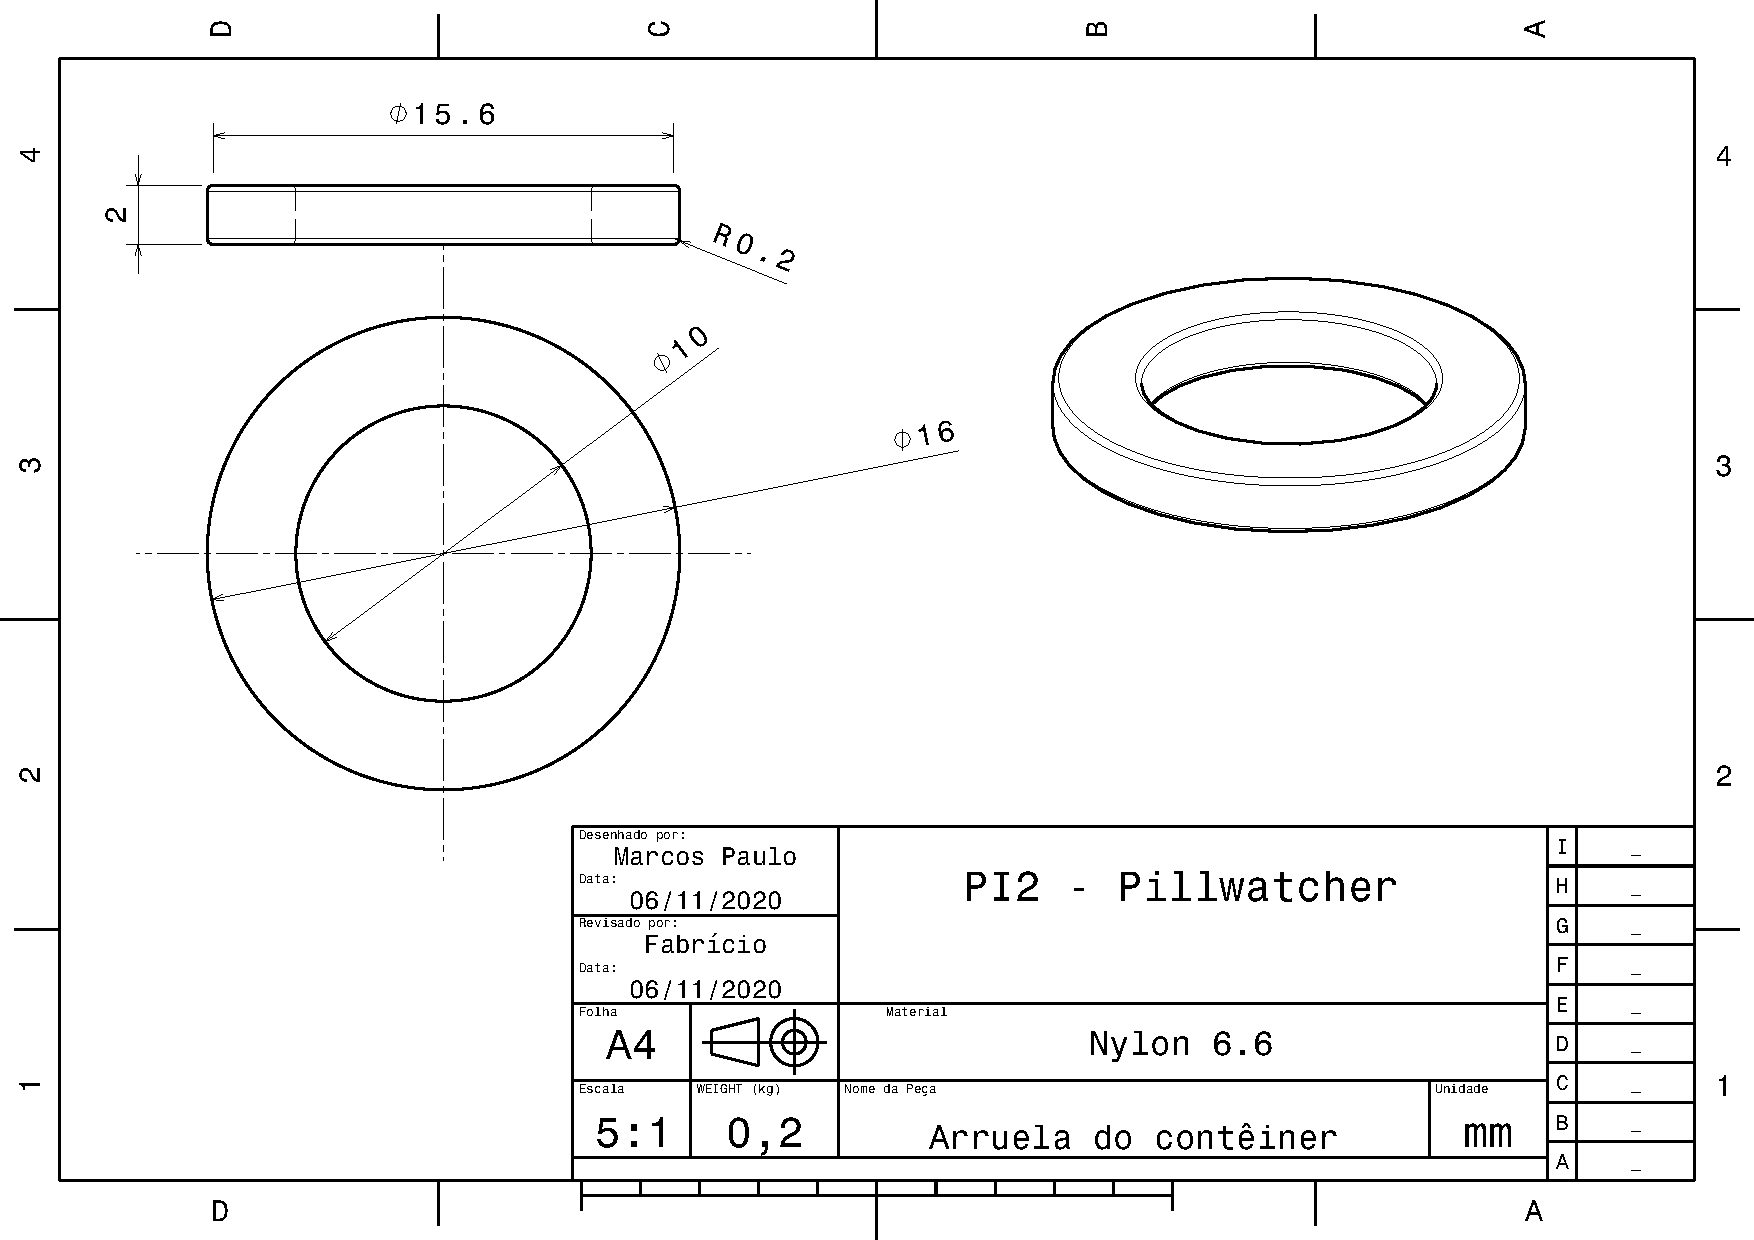
\includegraphics[width=0.9\textwidth]{figuras/estrutura/Desenhos/Arruela_conteiner.pdf}
    \caption{Desenho técnico da arruela do contêiner (\ref{retorno_engrenagem_fundo})}
    \label{fig:arruela}
\end{figure}

\begin{figure}[H]
    \centering
    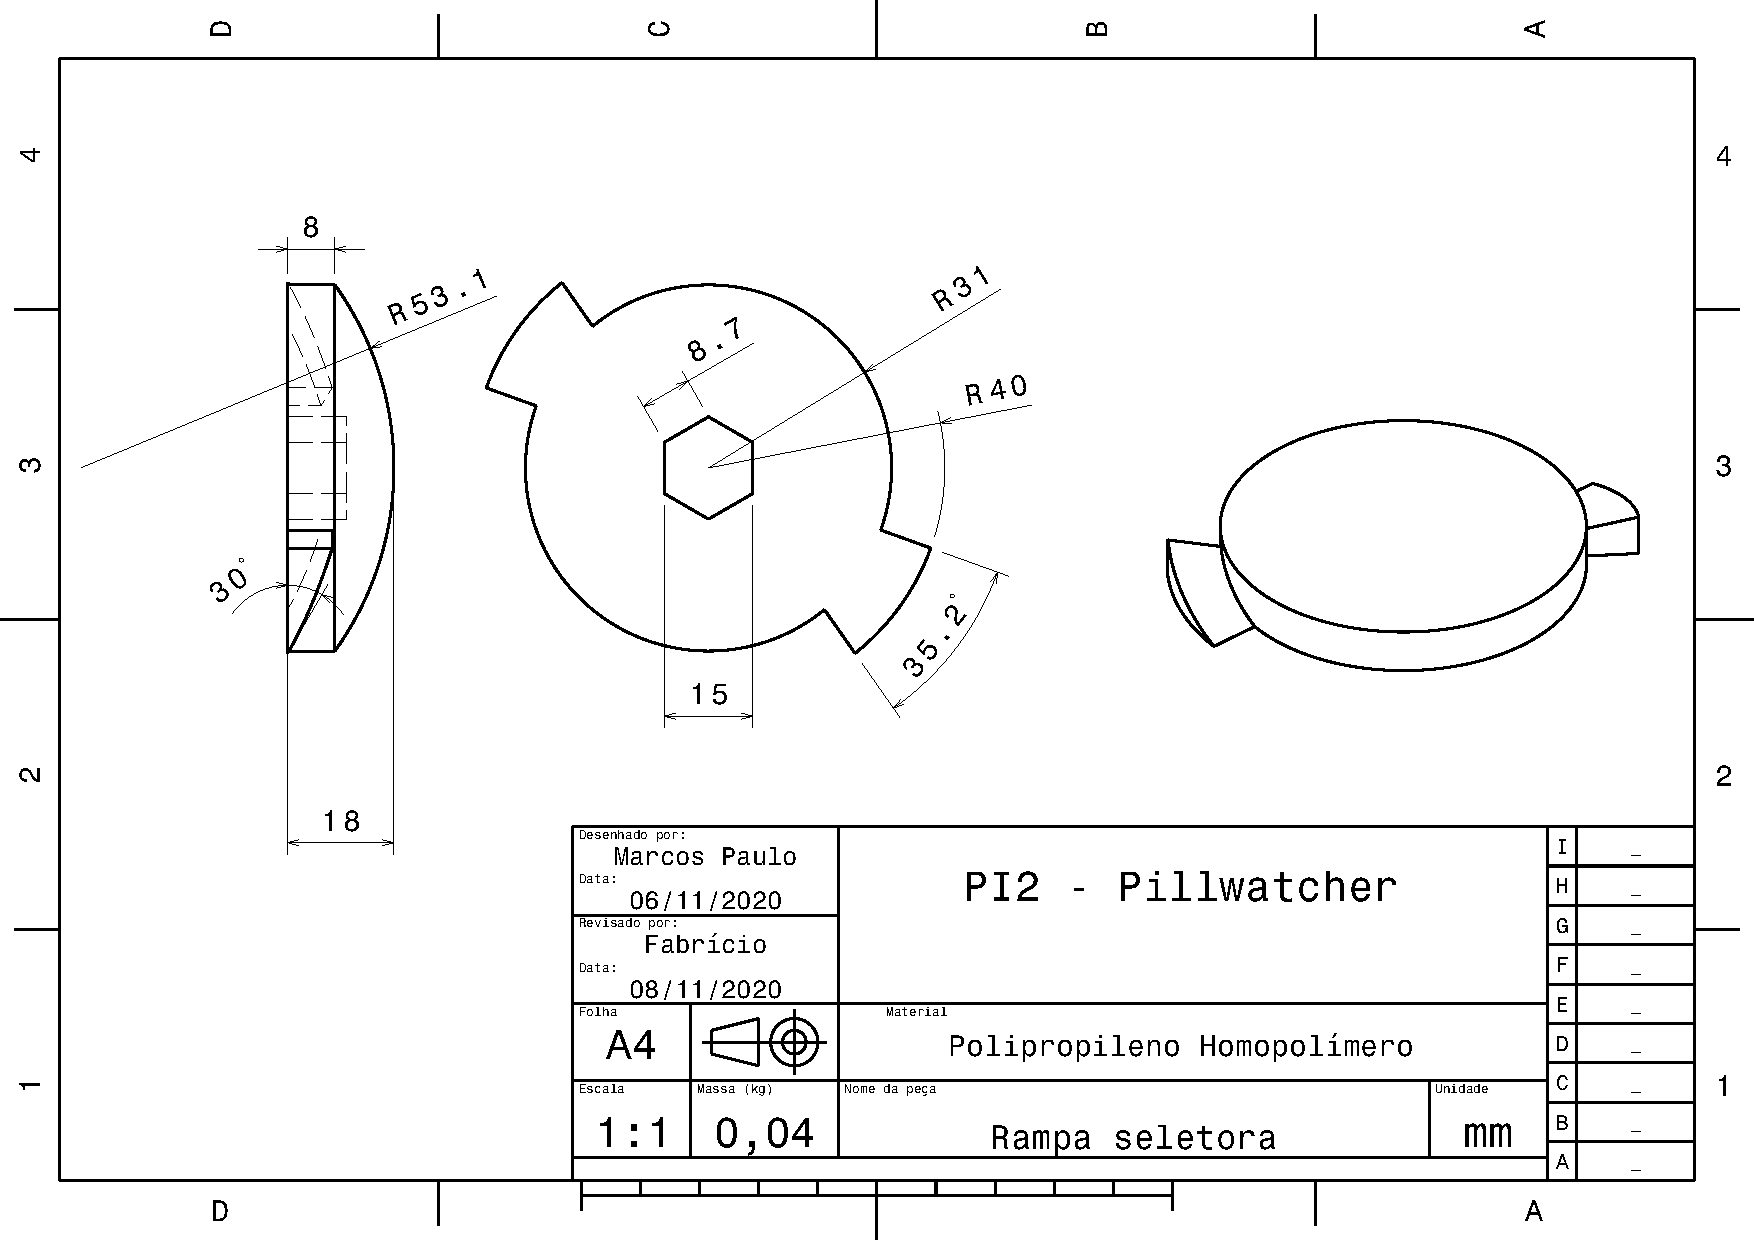
\includegraphics[width=0.9\textwidth]{figuras/estrutura/Desenhos/Rampa_Seletora.pdf}
    \caption{Desenho técnico das rampa seletora do contêiner (\ref{retorno_rampaseletora})}
    \label{fig:rampaseletora}
\end{figure}

\begin{figure}[H]
    \centering
    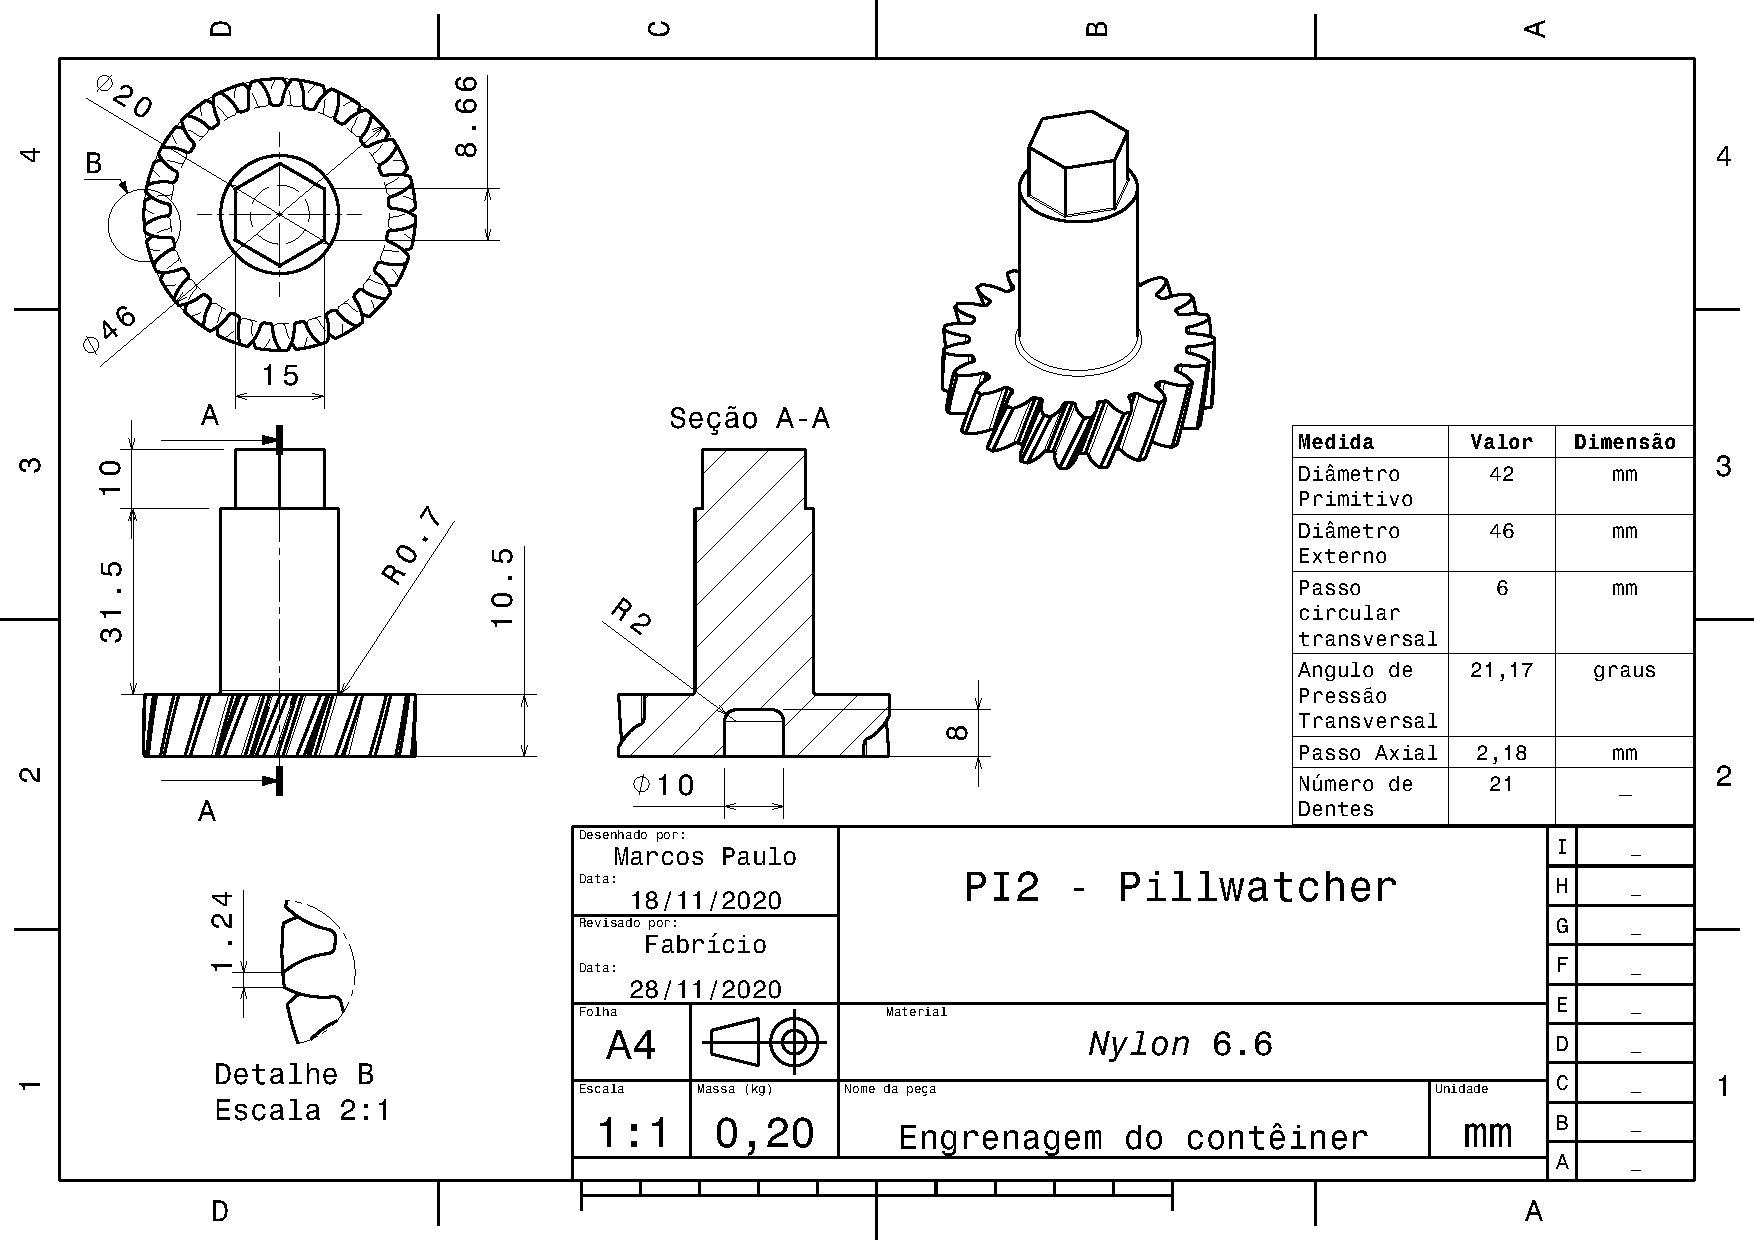
\includegraphics[width=0.9\textwidth]{figuras/estrutura/Desenhos/Engrenagem_Container_V2.1.pdf}
    \caption{Desenho técnico da engrenagem do contêiner (\ref{retorno_engrenagem_fundo})}
    \label{fig:engrenagem_fundo}
\end{figure}


\begin{figure}[H]
    \centering
    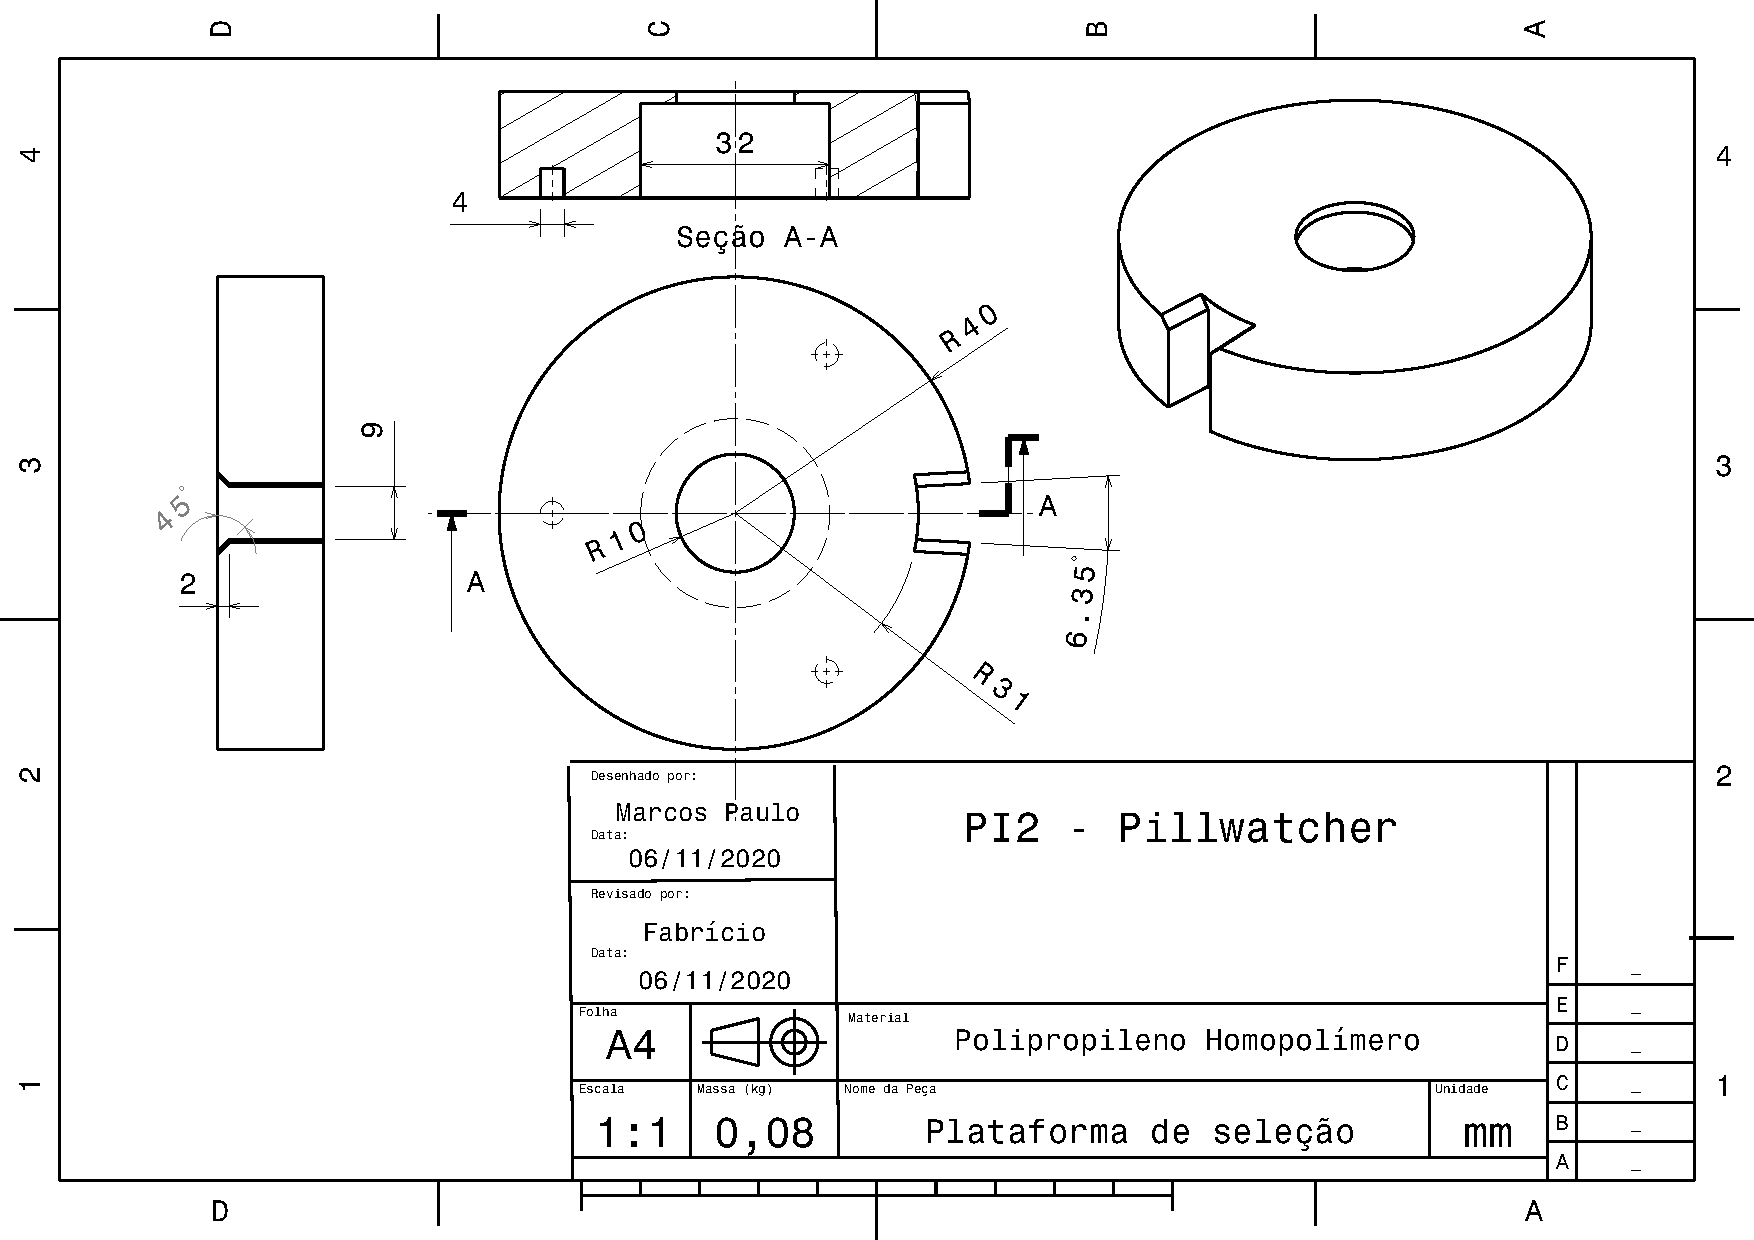
\includegraphics[width=0.9\textwidth]{figuras/estrutura/Desenhos/Plataforma_de_Selecao.pdf}
    \caption{Desenho técnico da plataforma de seleção(\ref{retorno_platosuperior})}
    \label{fig:platosuperior}
\end{figure}

\begin{figure}[H]
    \centering
    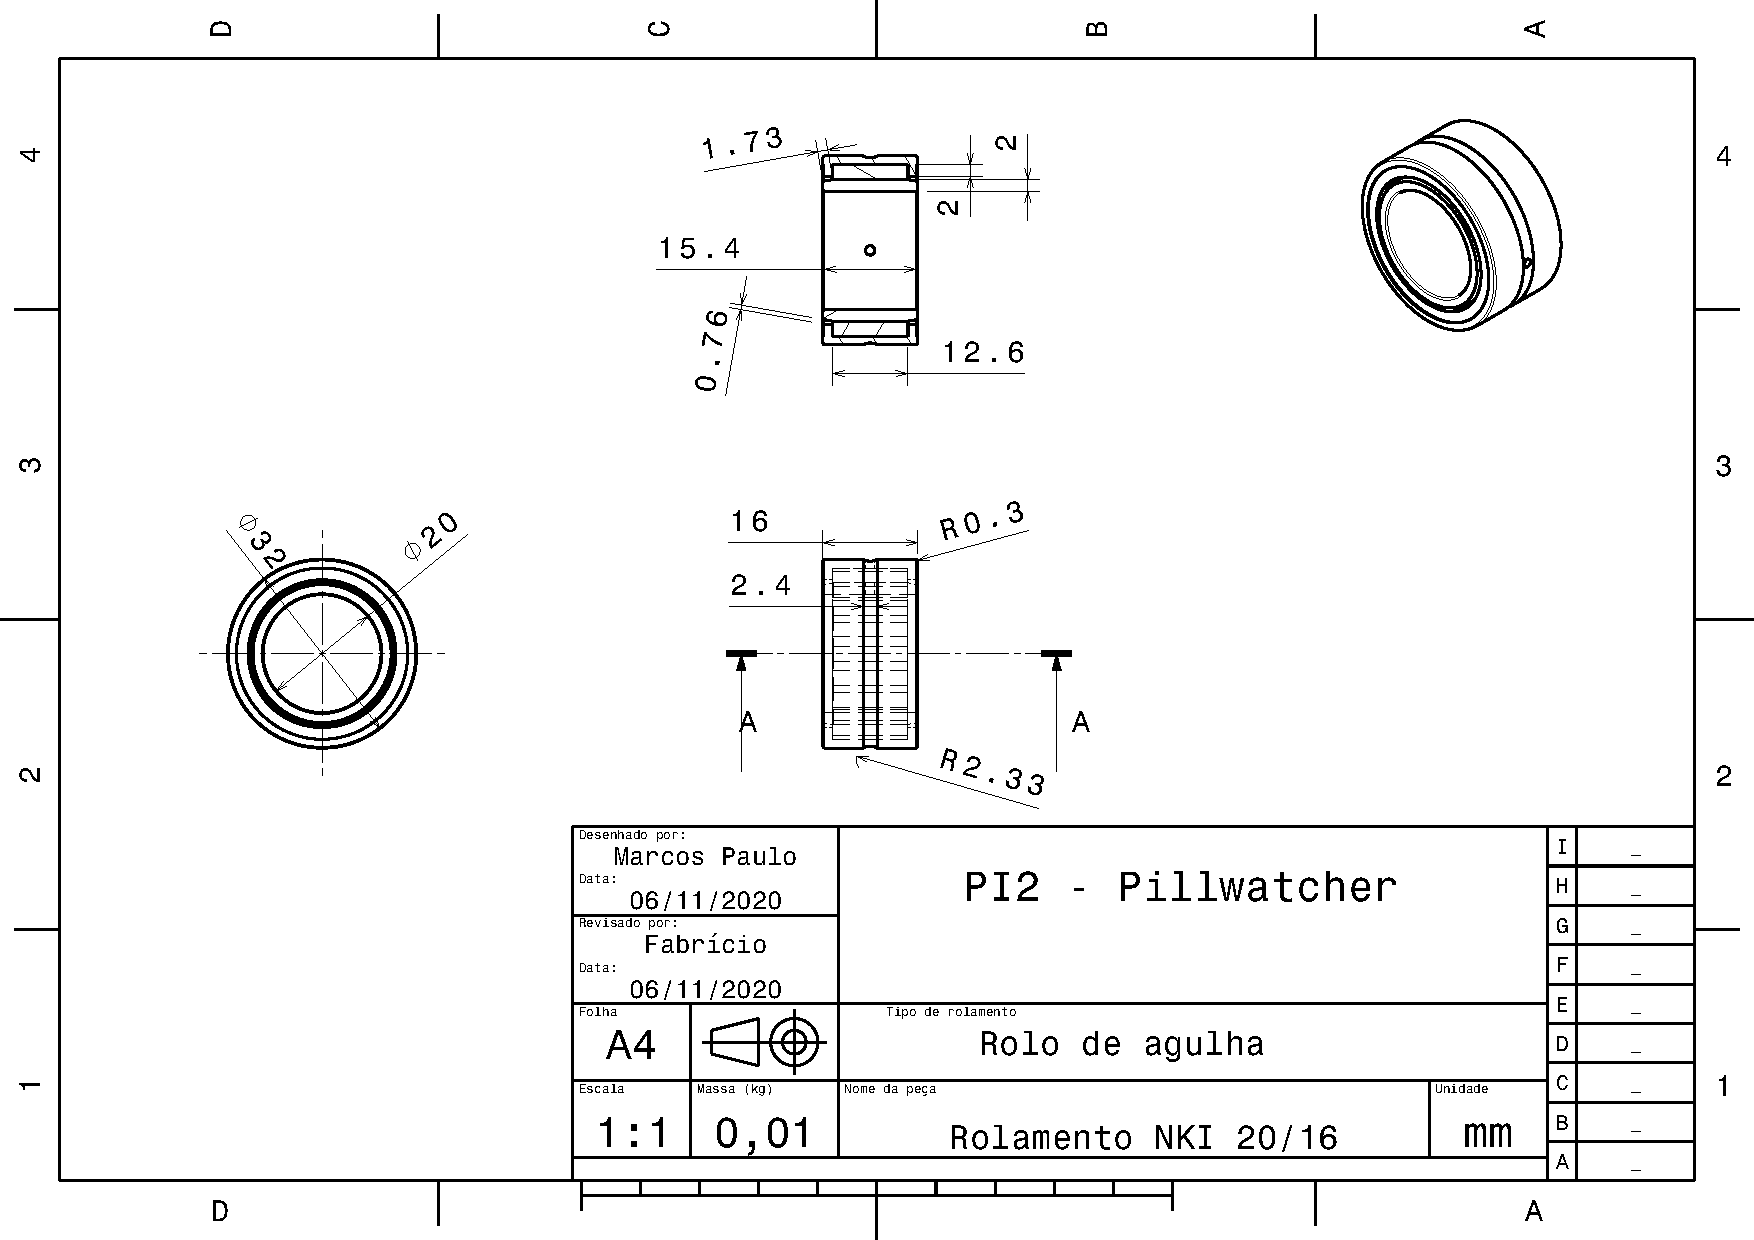
\includegraphics[width=0.9\textwidth]{figuras/estrutura/Desenhos/Rolamento_engrenagem.pdf}
    \caption{Desenho técnico do rolamento da engrenagem (\ref{retorno_engrenagem_fundo})}
    \label{fig:rolamento_engrenagem}
\end{figure}

\begin{figure}[H]
    \centering
    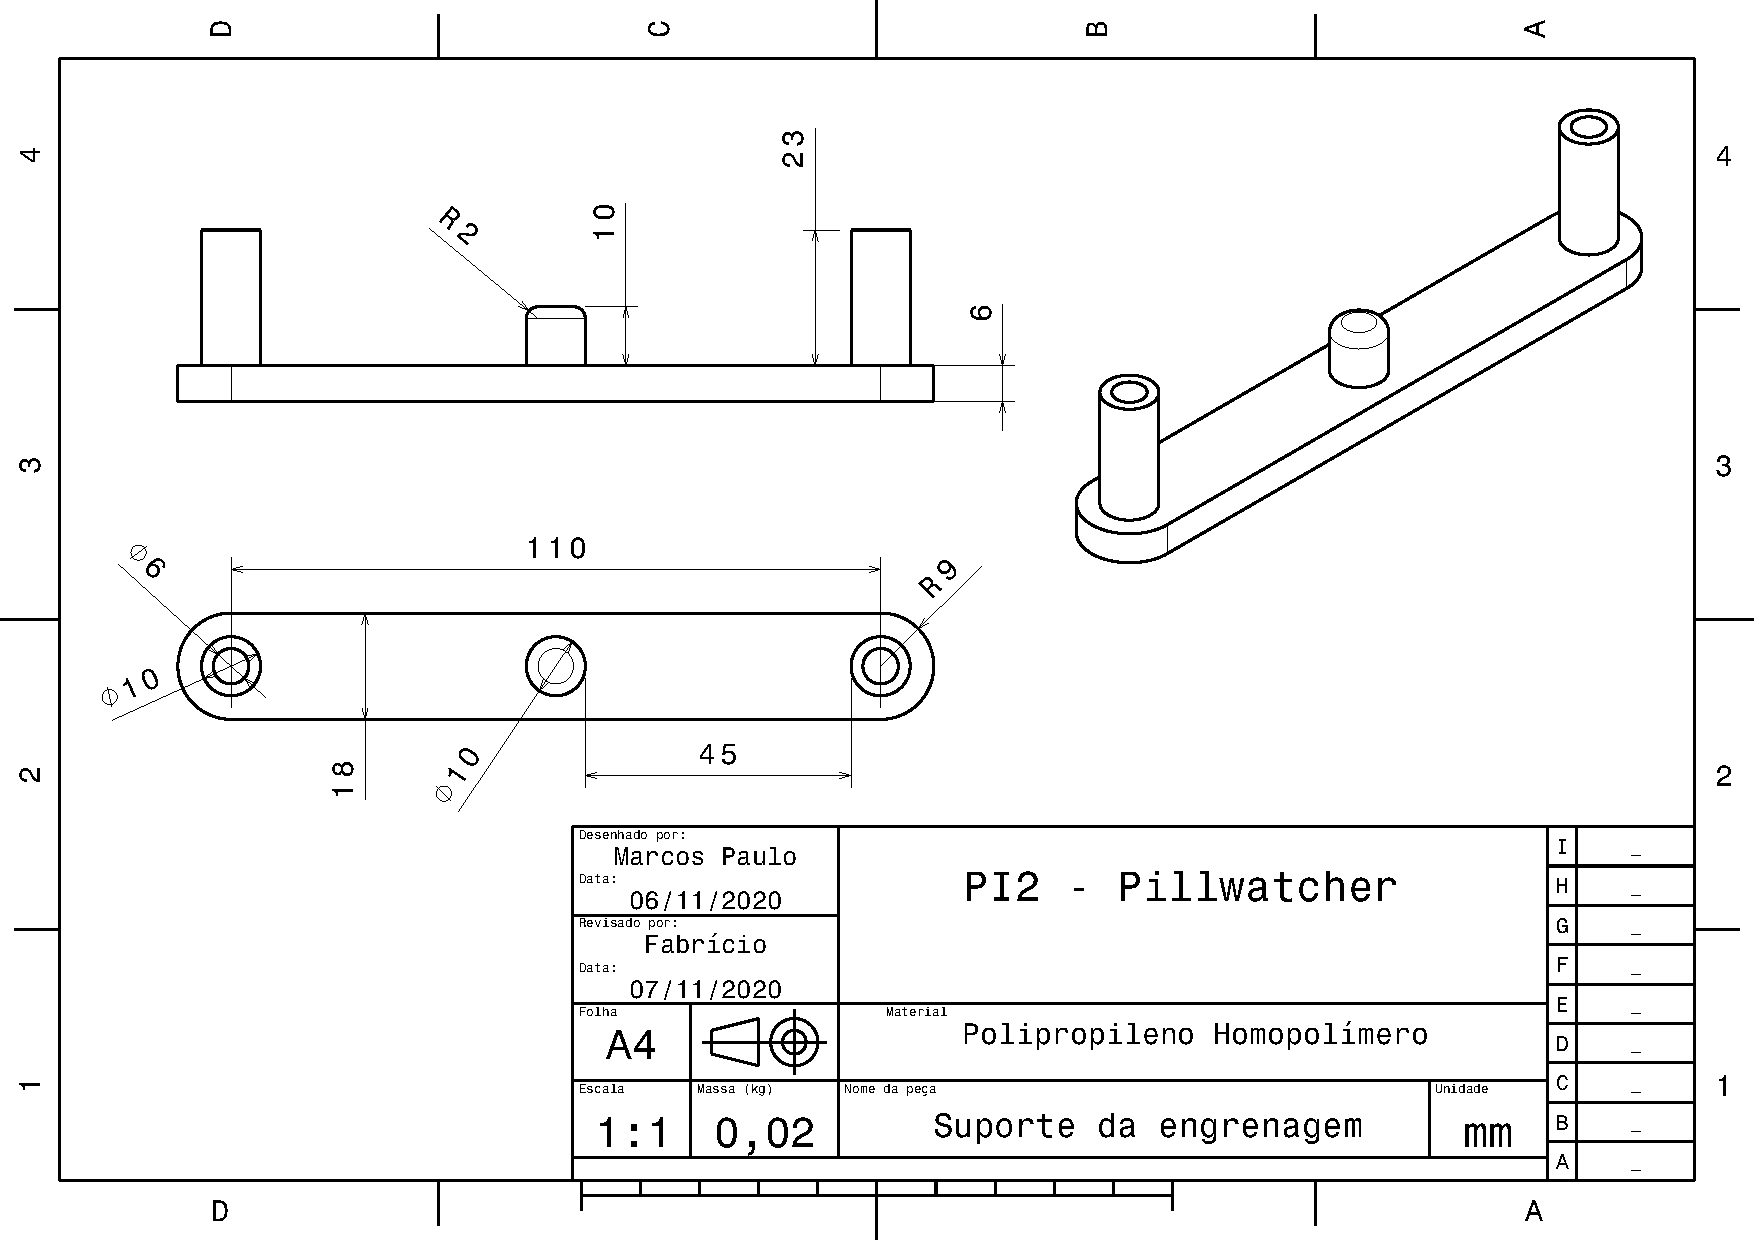
\includegraphics[width=0.9\textwidth]{figuras/estrutura/Desenhos/Suporte_Engrenagem_Container.pdf}
    \caption{Desenho técnico do suporte da engrenagem no contêiner (\ref{retorno_suporte_engrenagem})}
    \label{fig:supp_engrenagem}
\end{figure}

\begin{figure}[H]
    \centering
    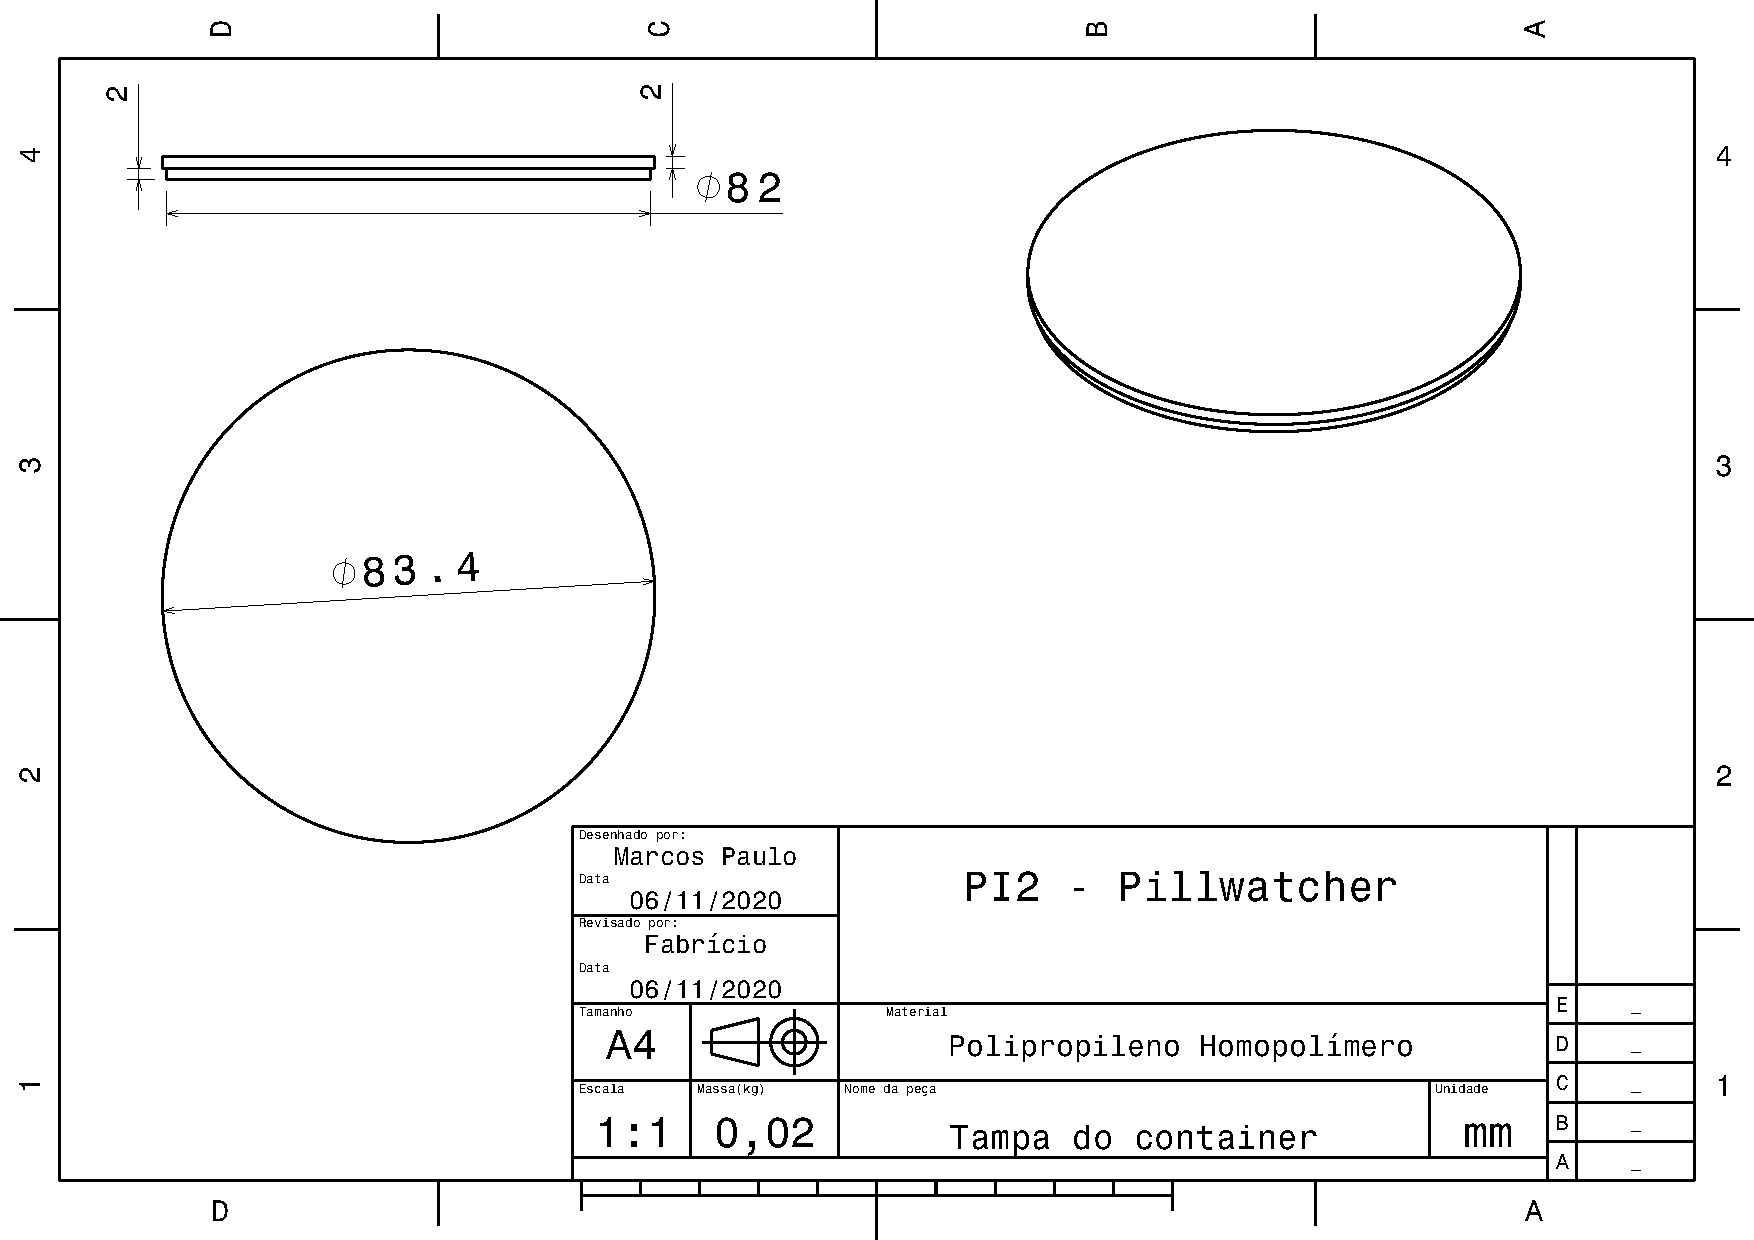
\includegraphics[width=0.9\textwidth]{figuras/estrutura/Desenhos/Tampa_Container.pdf}
    \caption{Desenho técnico da tampa do contêiner (\ref{retorno_tampa})}
    \label{fig:tampa}
\end{figure}

\begin{figure}[H]
    \centering
    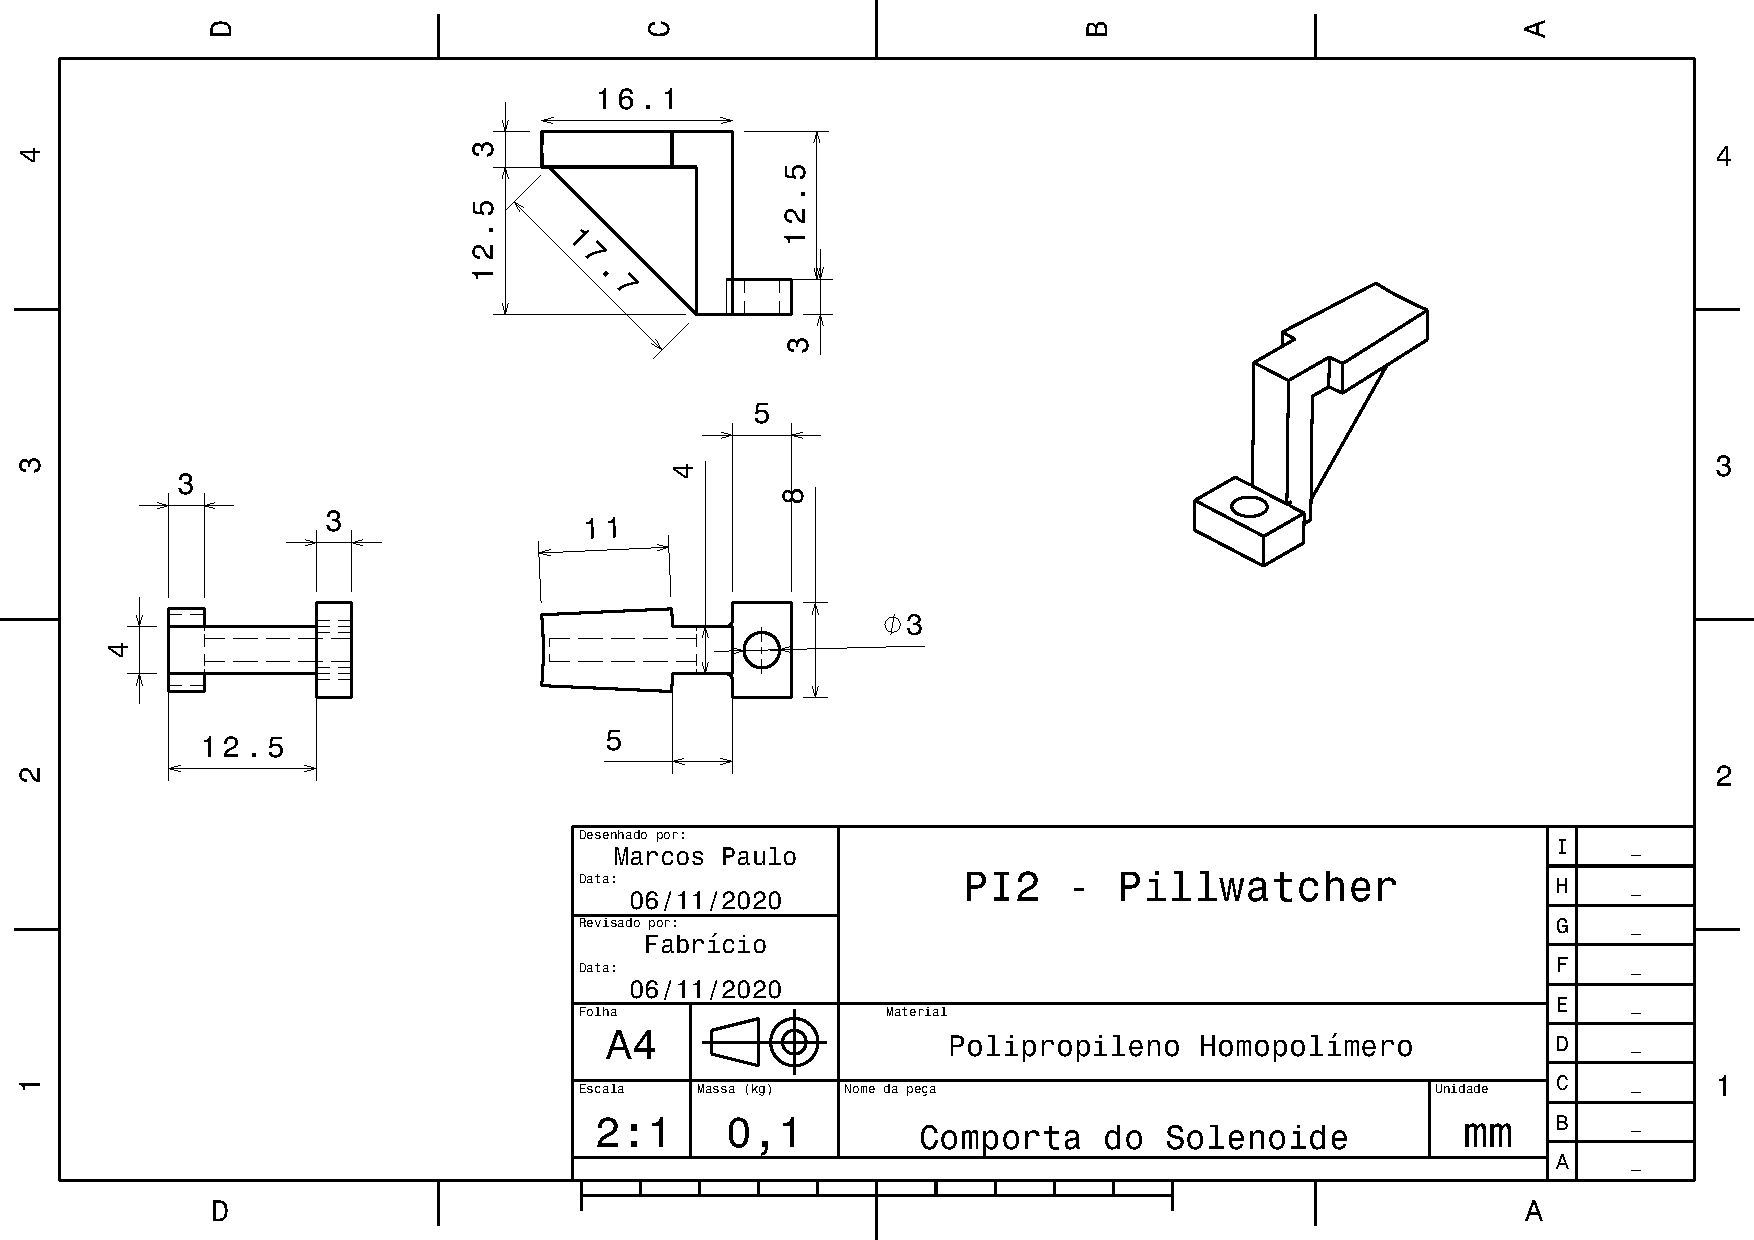
\includegraphics[width=0.9\textwidth]{figuras/estrutura/Desenhos/Comporta_Solenoide.pdf}
    \caption{Desenho técnico da comporta do contêiner (\ref{retorno_comporta})}
    \label{fig:comporta}
\end{figure}

\begin{figure}[H]
    \centering
    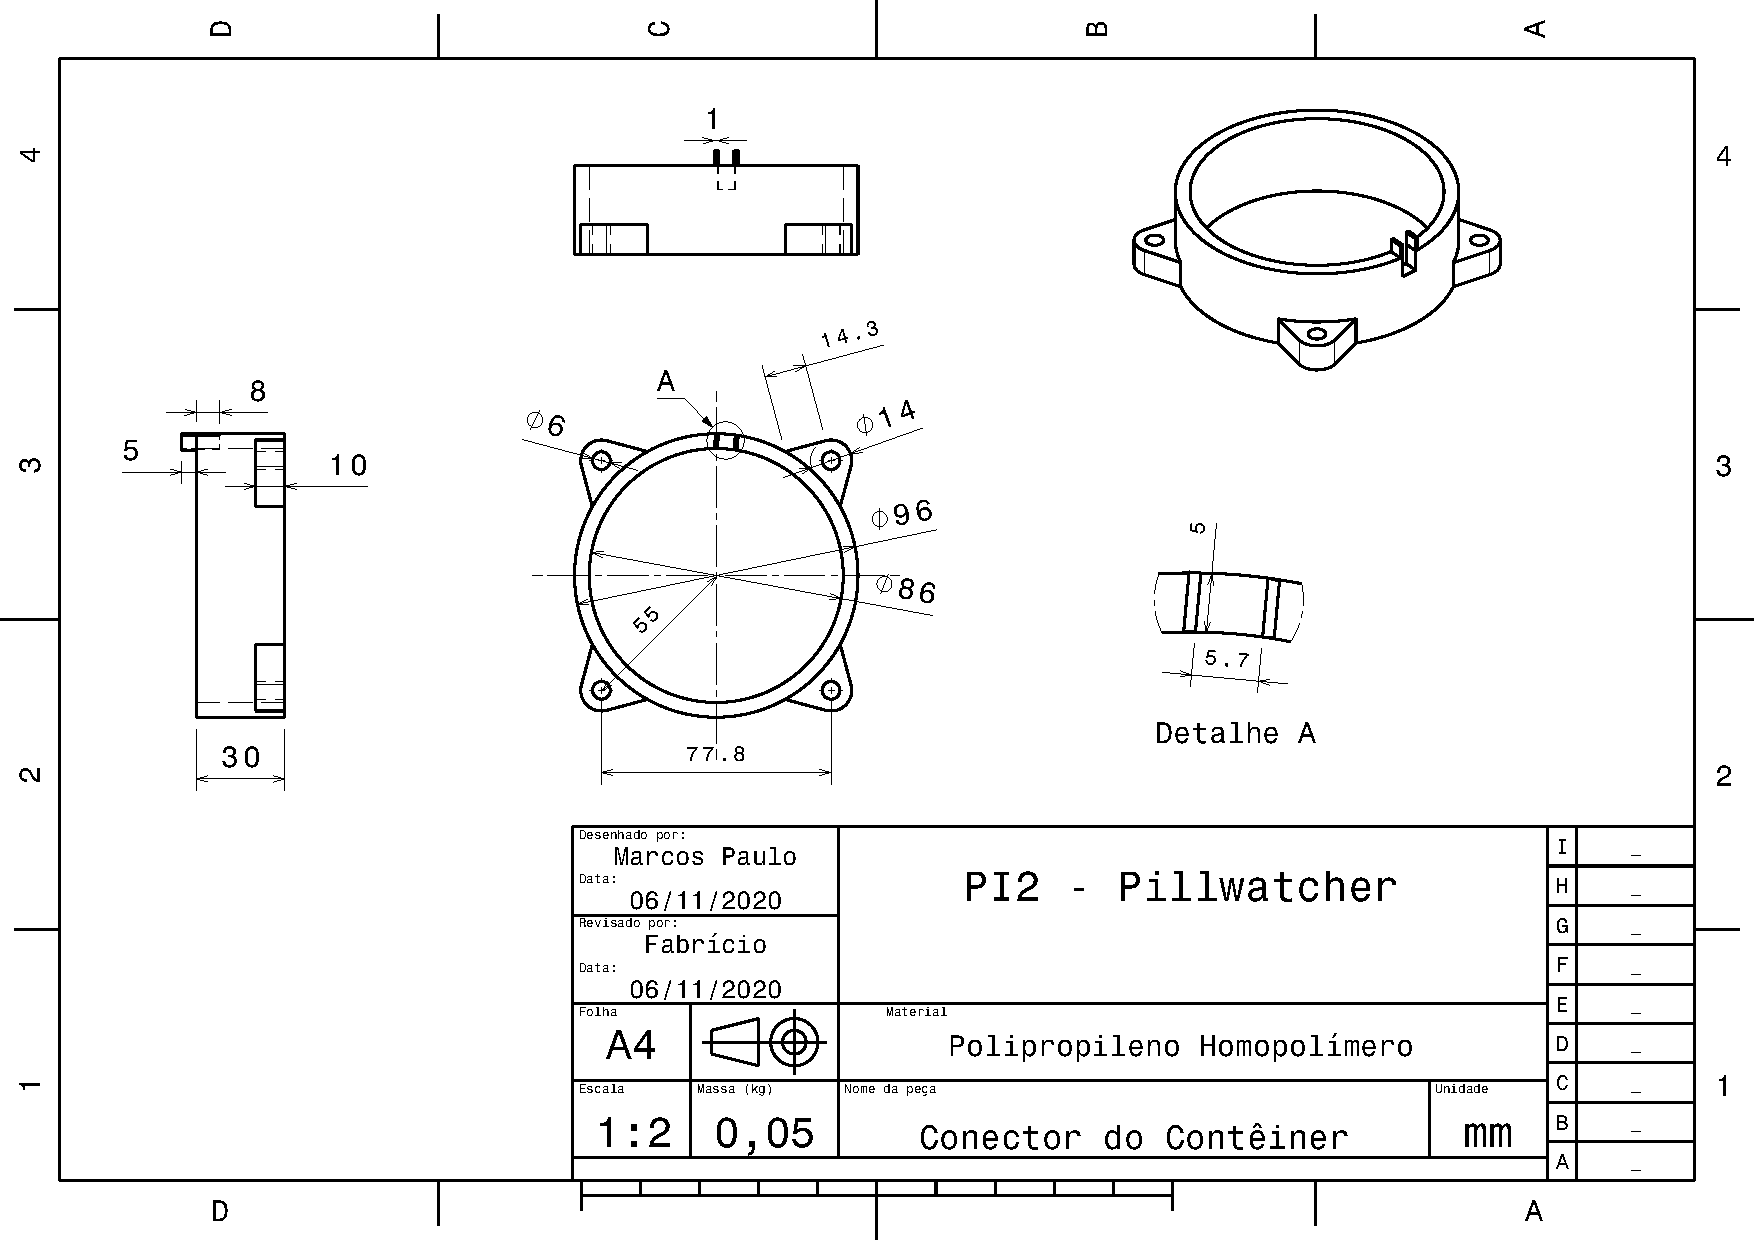
\includegraphics[width=0.9\textwidth]{figuras/estrutura/Desenhos/ConectorContainer.pdf}
    \caption{Desenho técnico do conector do contêiner à base (\ref{retorno_conector})}
    \label{fig:conector}
\end{figure}

\begin{figure}[H]
    \centering
    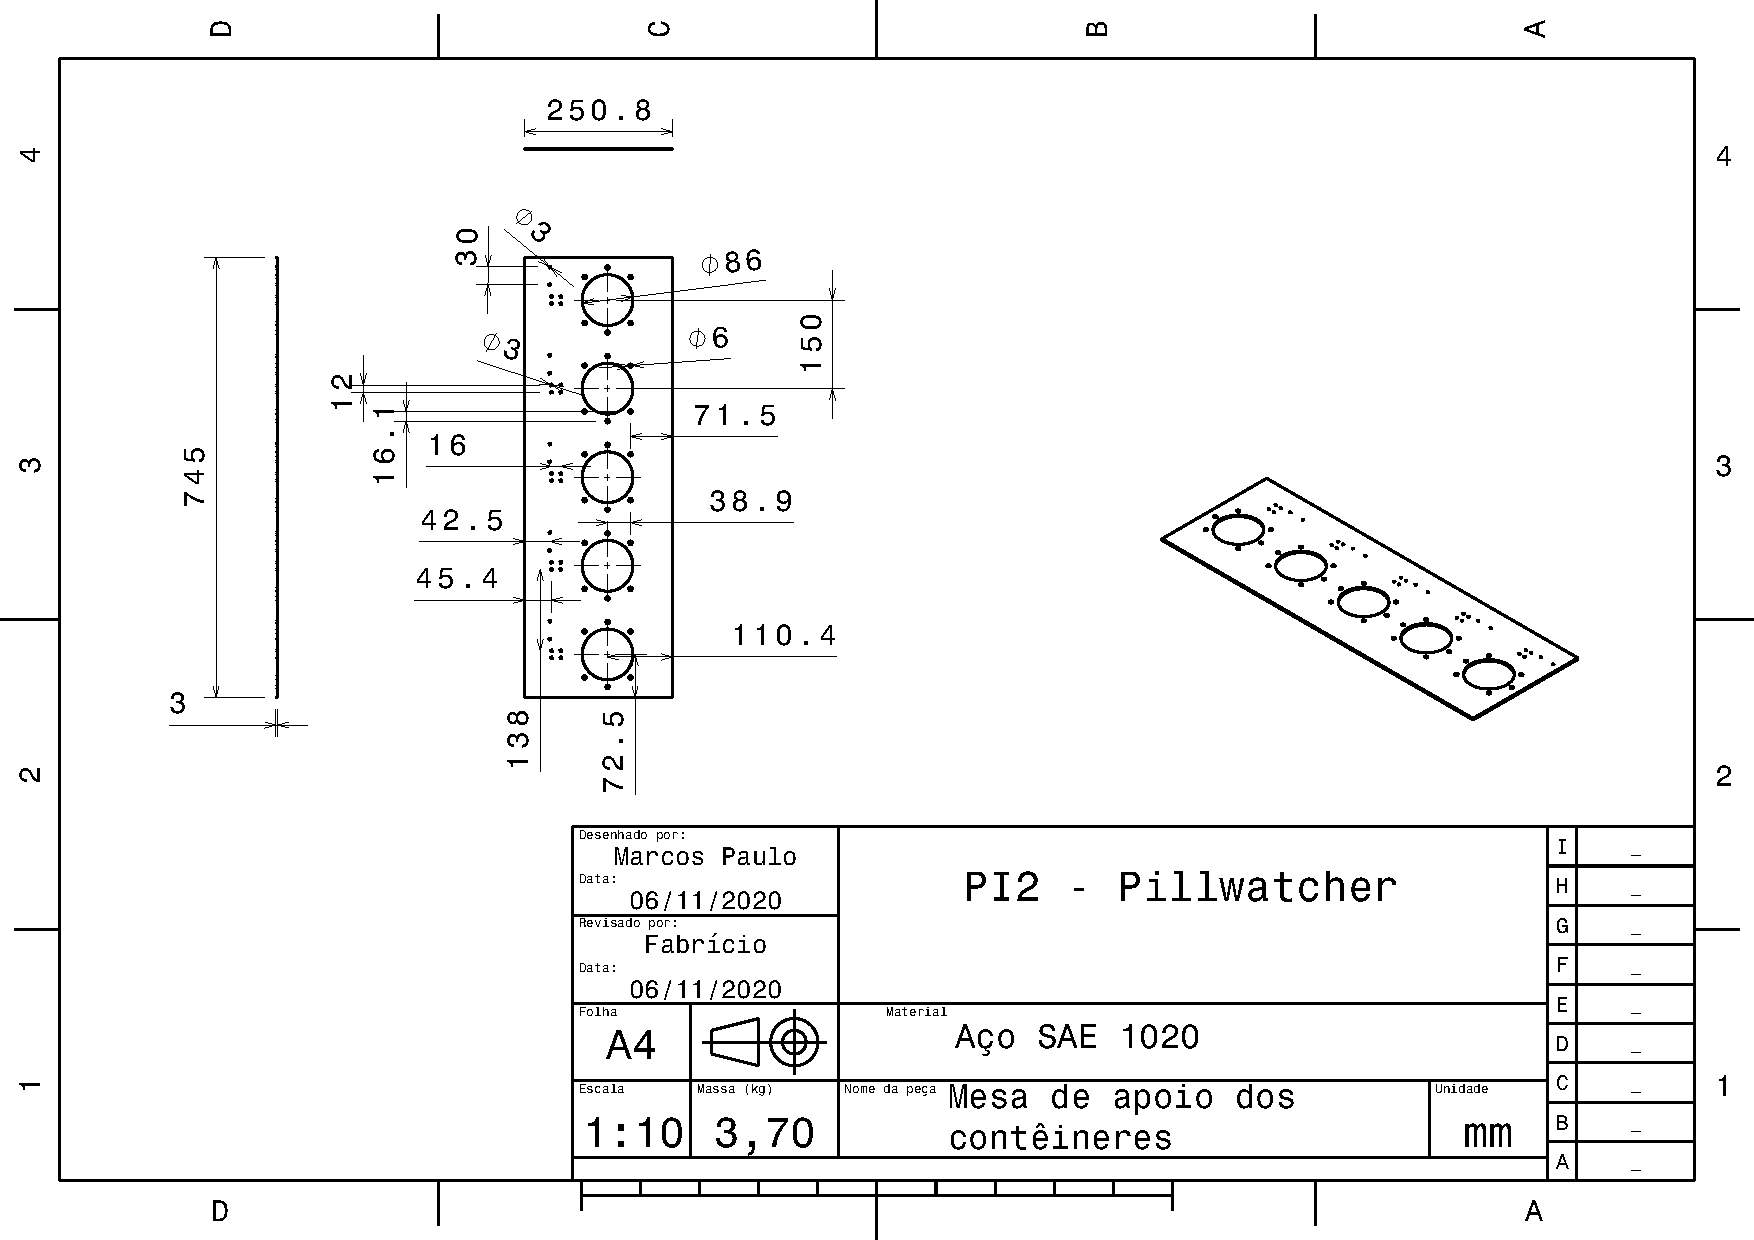
\includegraphics[width=0.9\textwidth]{figuras/estrutura/Desenhos/Base_Containers.pdf}
    \caption{Desenho técnico da base dos contêineres (\ref{retorno_base_subgrupo})}
    \label{fig:base_subgrupo}
\end{figure}

\begin{figure}[H]
    \centering
    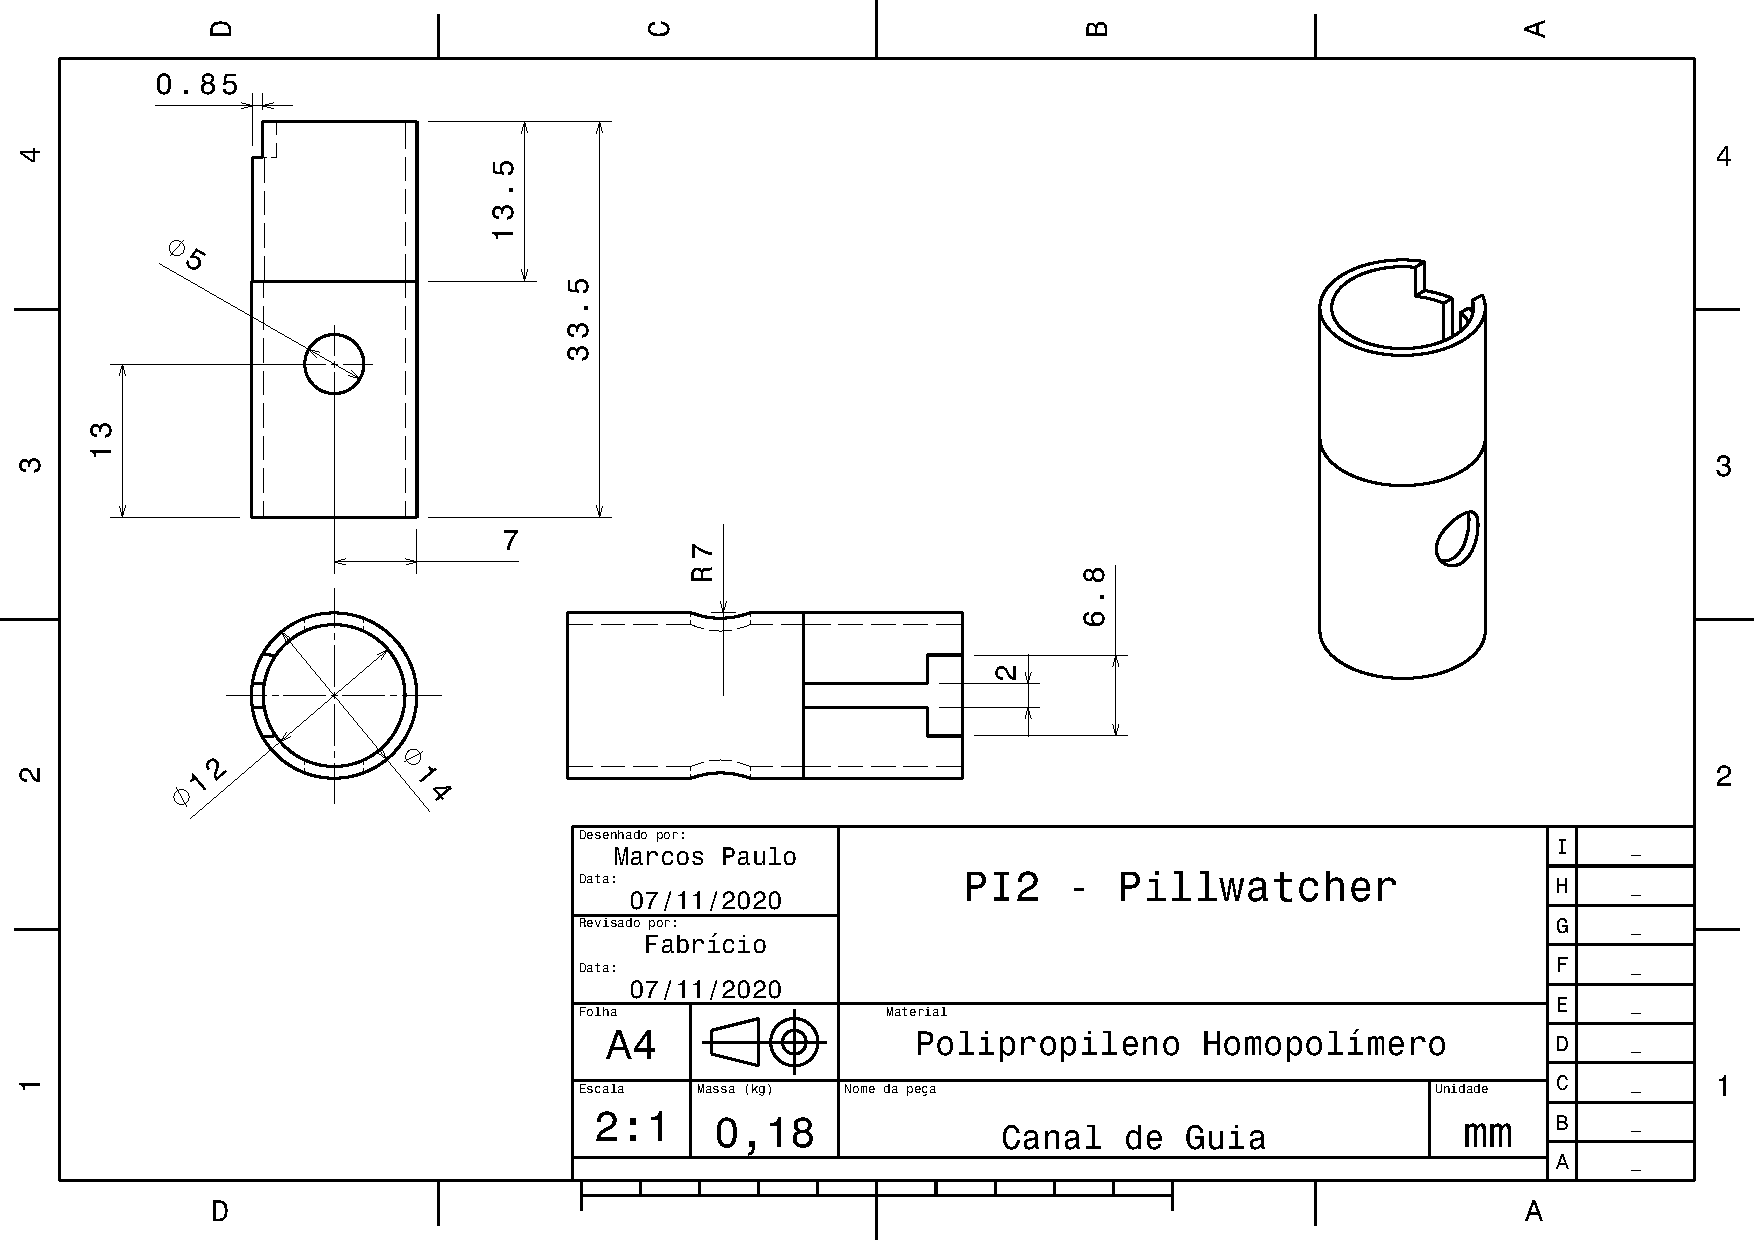
\includegraphics[width=0.9\textwidth]{figuras/estrutura/Desenhos/Canal de Guia.pdf}
    \caption{Desenho técnico do Canal de Guia (\ref{retorno_zonadetransição})}
    \label{fig:canalguia}
\end{figure}

\begin{figure}[H]
    \centering
    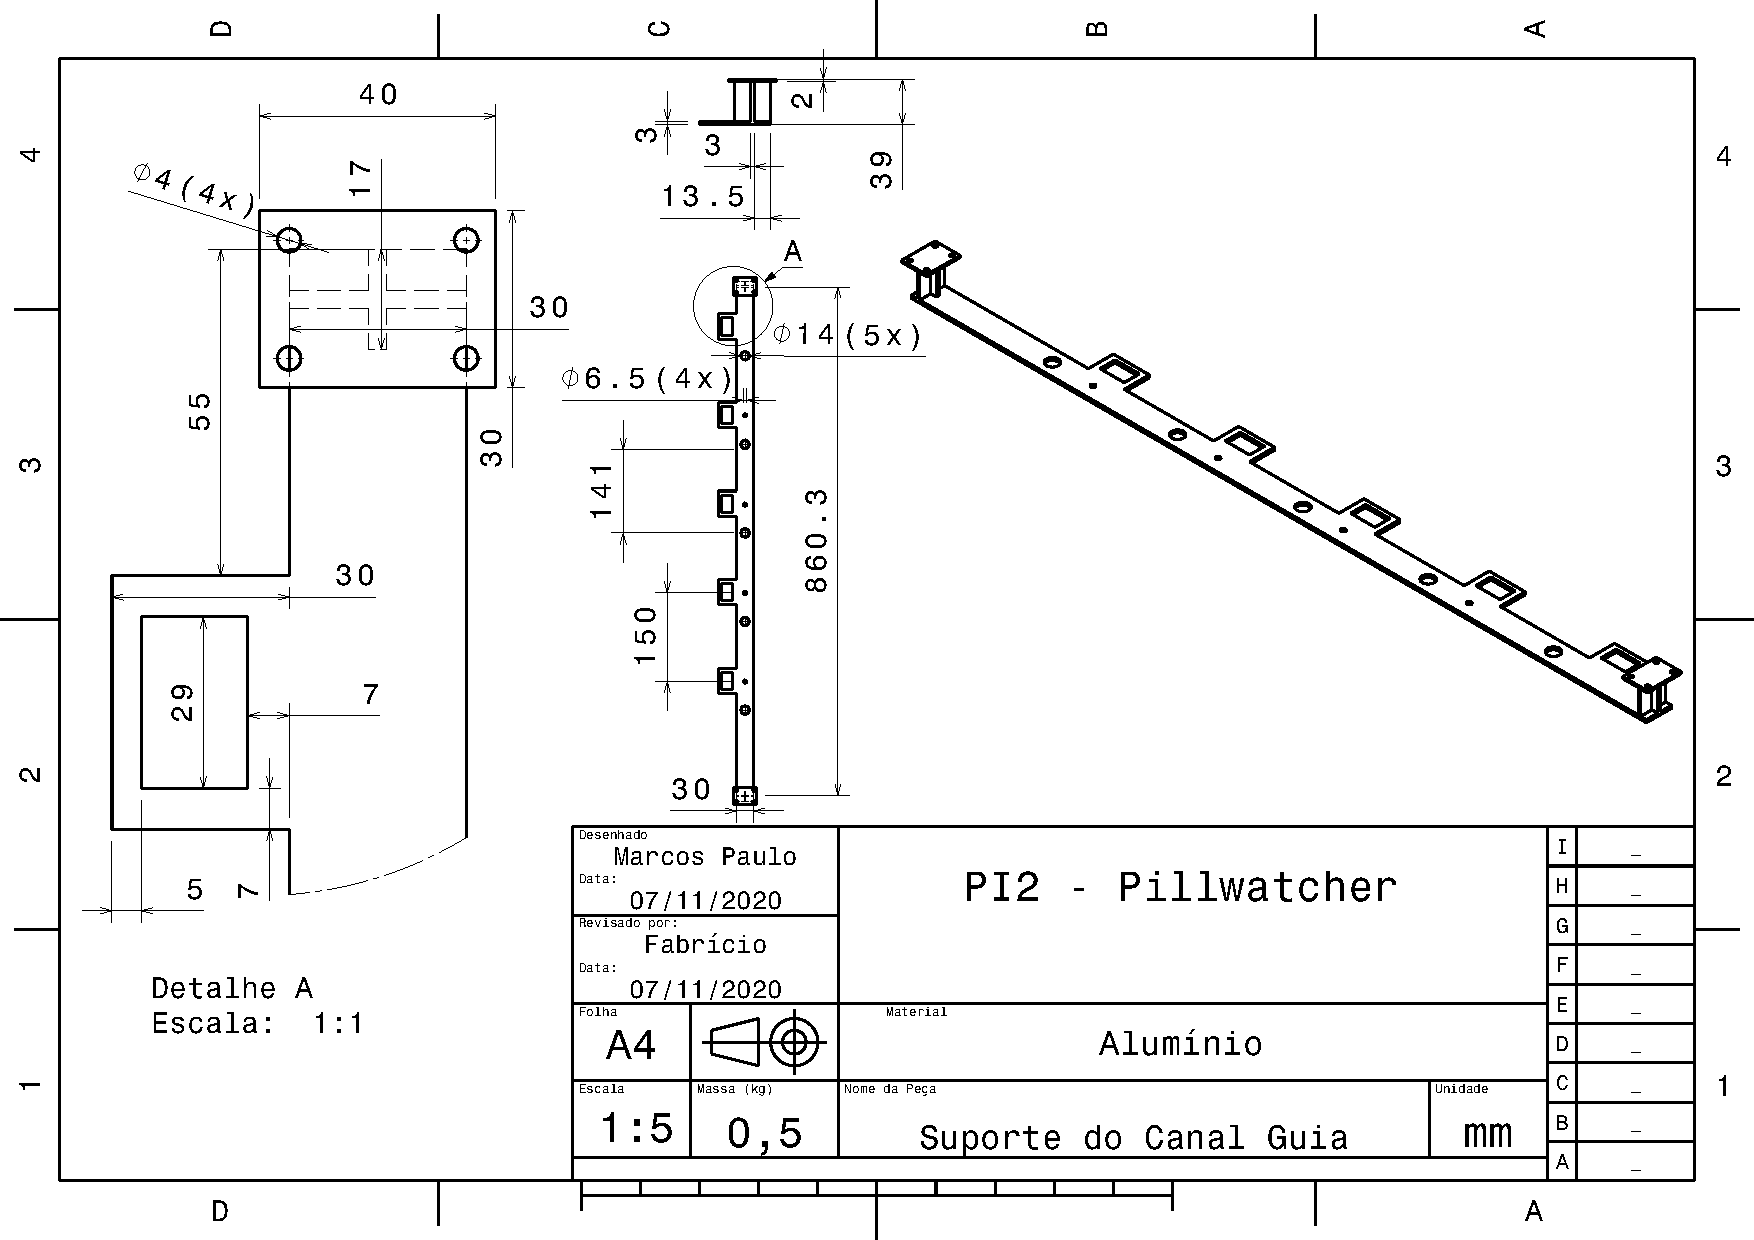
\includegraphics[width=0.9\textwidth]{figuras/estrutura/Desenhos/Suporte_Canal_Guia.pdf}
    \caption{Desenho técnico do suporte dos canais de guia (\ref{retorno_zonadetransição})}
    \label{fig:supp_canal}
\end{figure}

\begin{figure}[H]
    \centering
    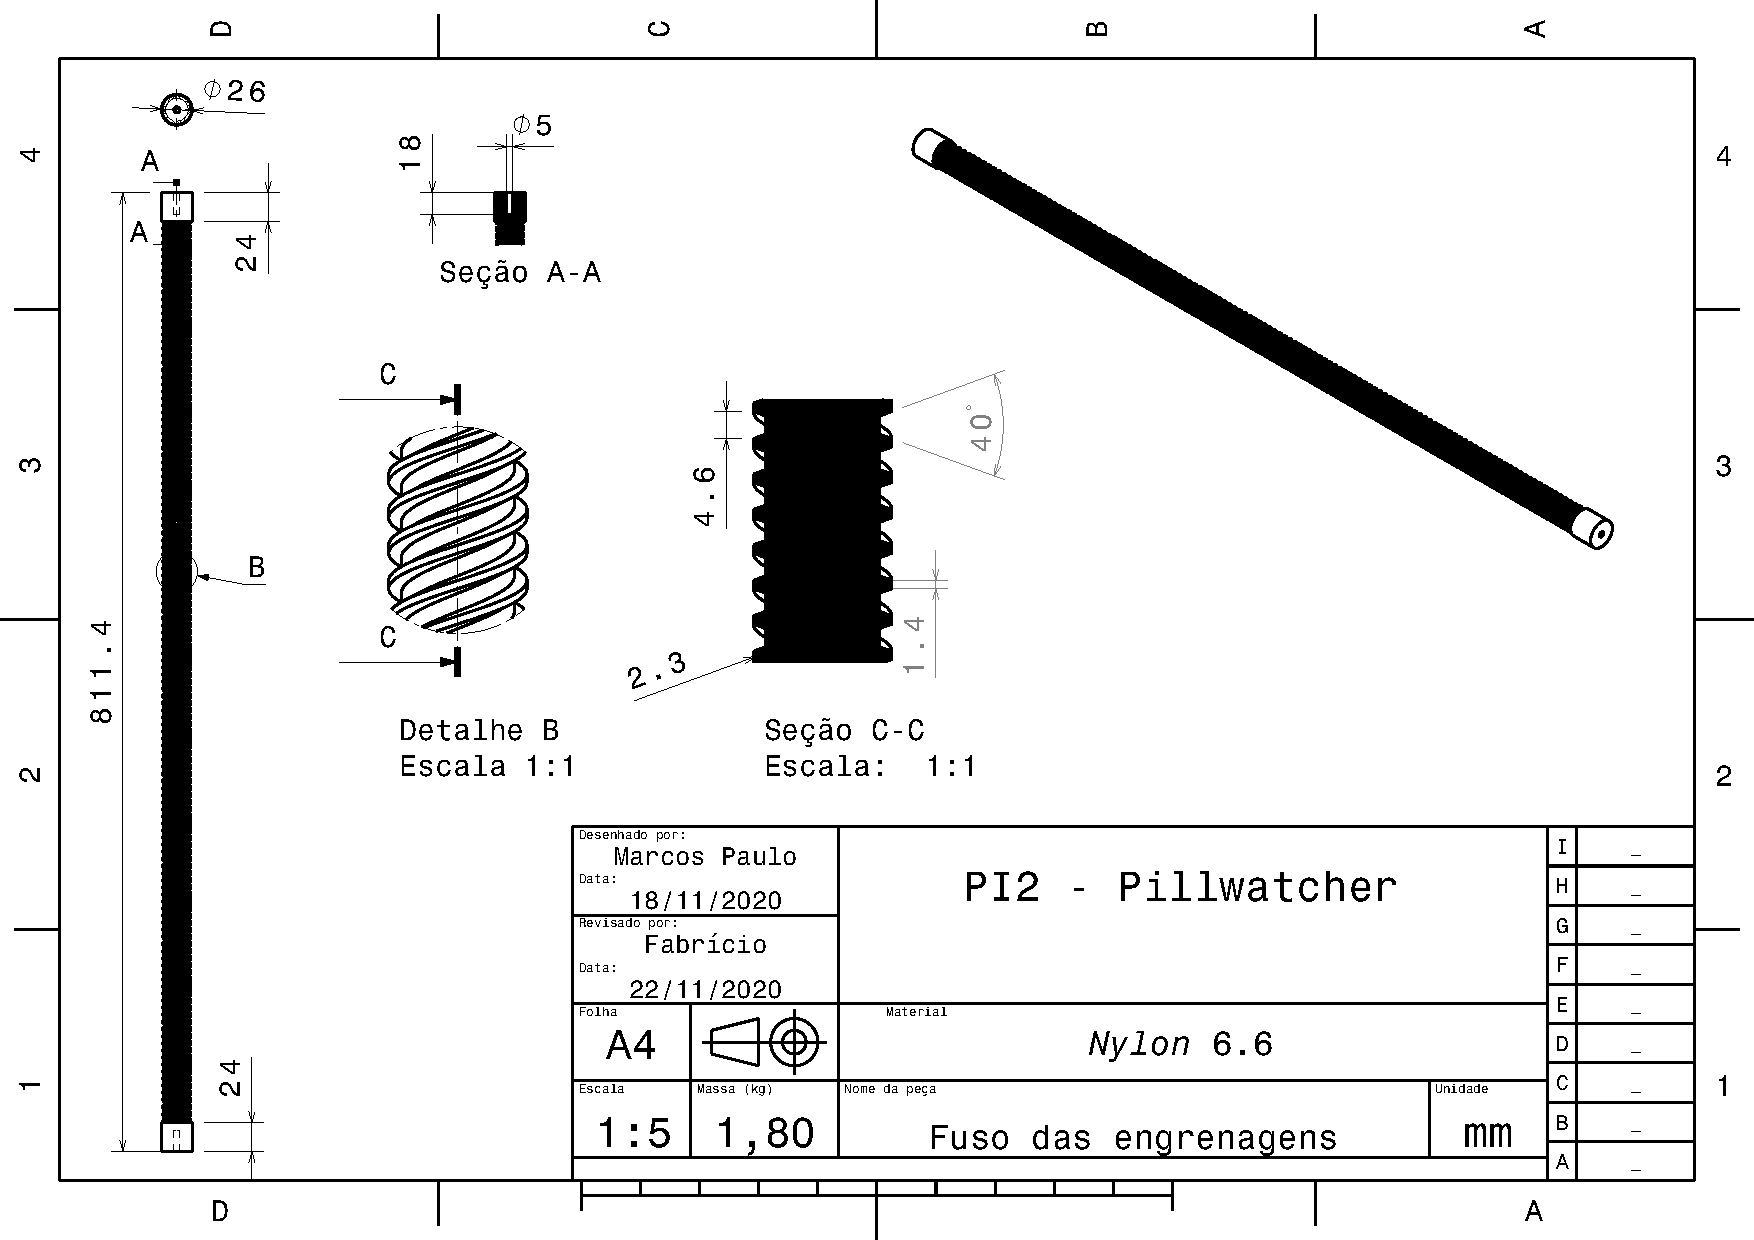
\includegraphics[width=0.9\textwidth]{figuras/estrutura/Desenhos/Fuso_Engrenagens_V2.pdf}
    \caption{Desenho técnico do fuso de atuação nas engrenagens (\ref{retorno_fuso})}
    \label{fig:fuso}
\end{figure}

\begin{figure}[H]
    \centering
    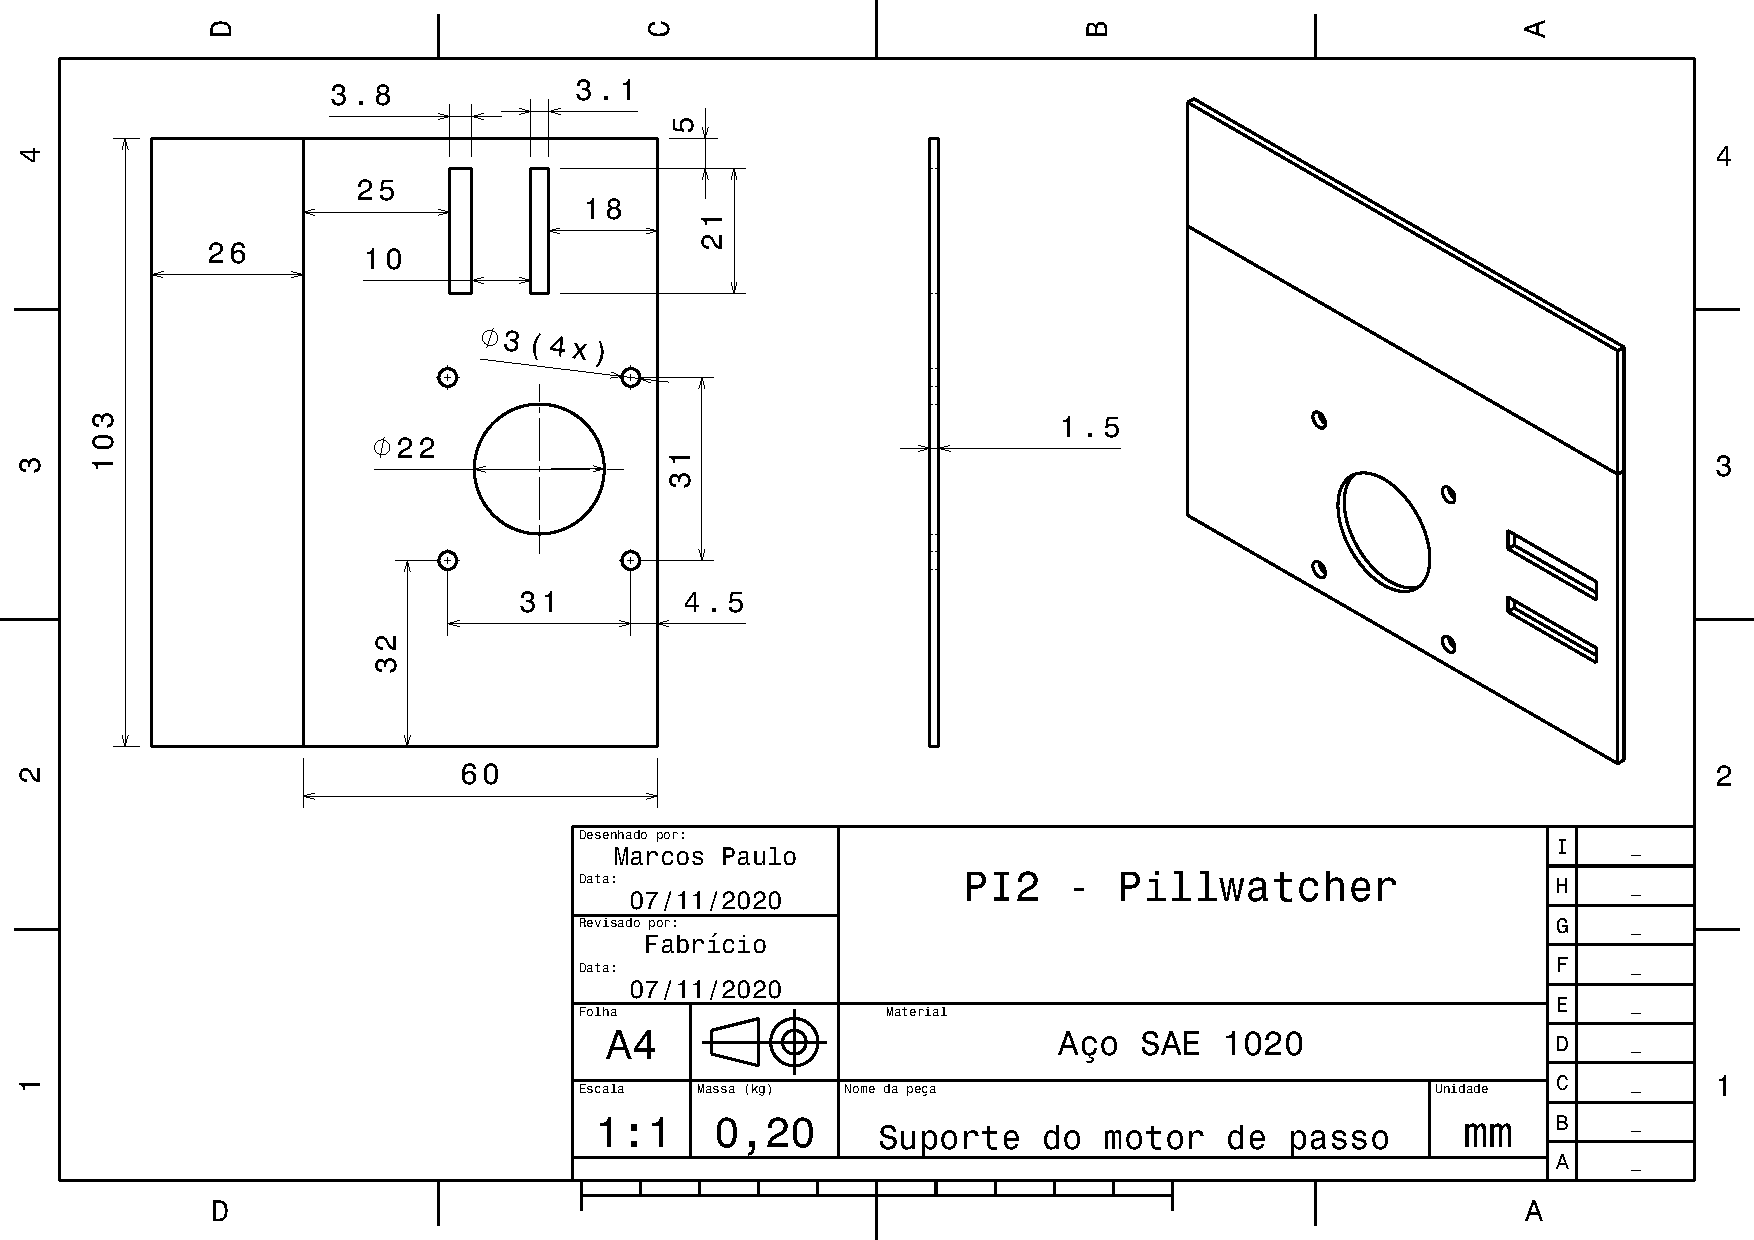
\includegraphics[width=0.9\textwidth]{figuras/estrutura/Desenhos/Suporte_Motor_Passo.pdf}
    \caption{Desenho técnico do suporte dos motores de passo (\ref{retorno_suporte_motordepasso})}
    \label{fig:supp_motordepasso}
\end{figure}

\begin{figure}[H]
    \centering
    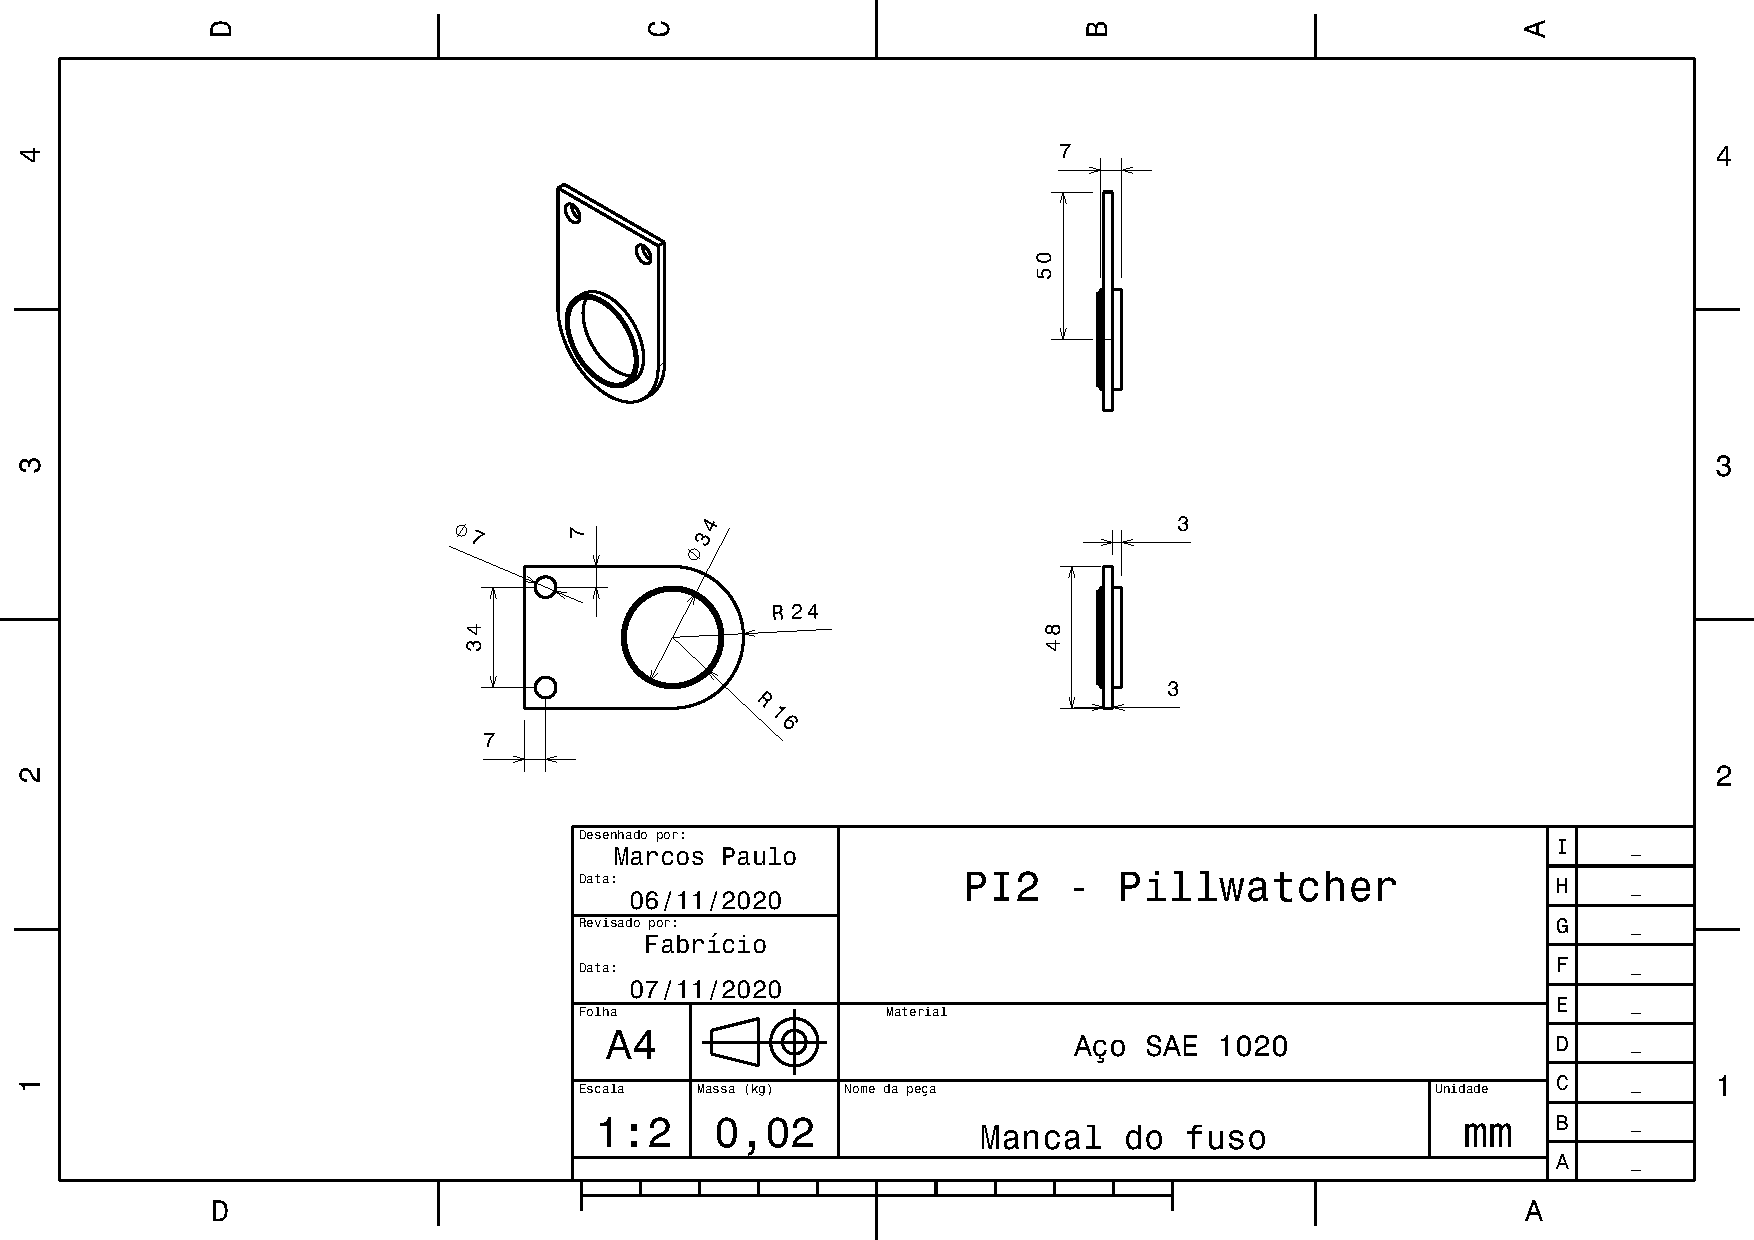
\includegraphics[width=0.9\textwidth]{figuras/estrutura/Desenhos/Mancal_Fuso.pdf}
    \caption{Desenho técnico do mancal de apoio do fuso (\ref{Retorno_Mancal_de_suporte})}
    \label{fig:Mancal_Fuso}
\end{figure}

\begin{figure}[H]
    \centering
    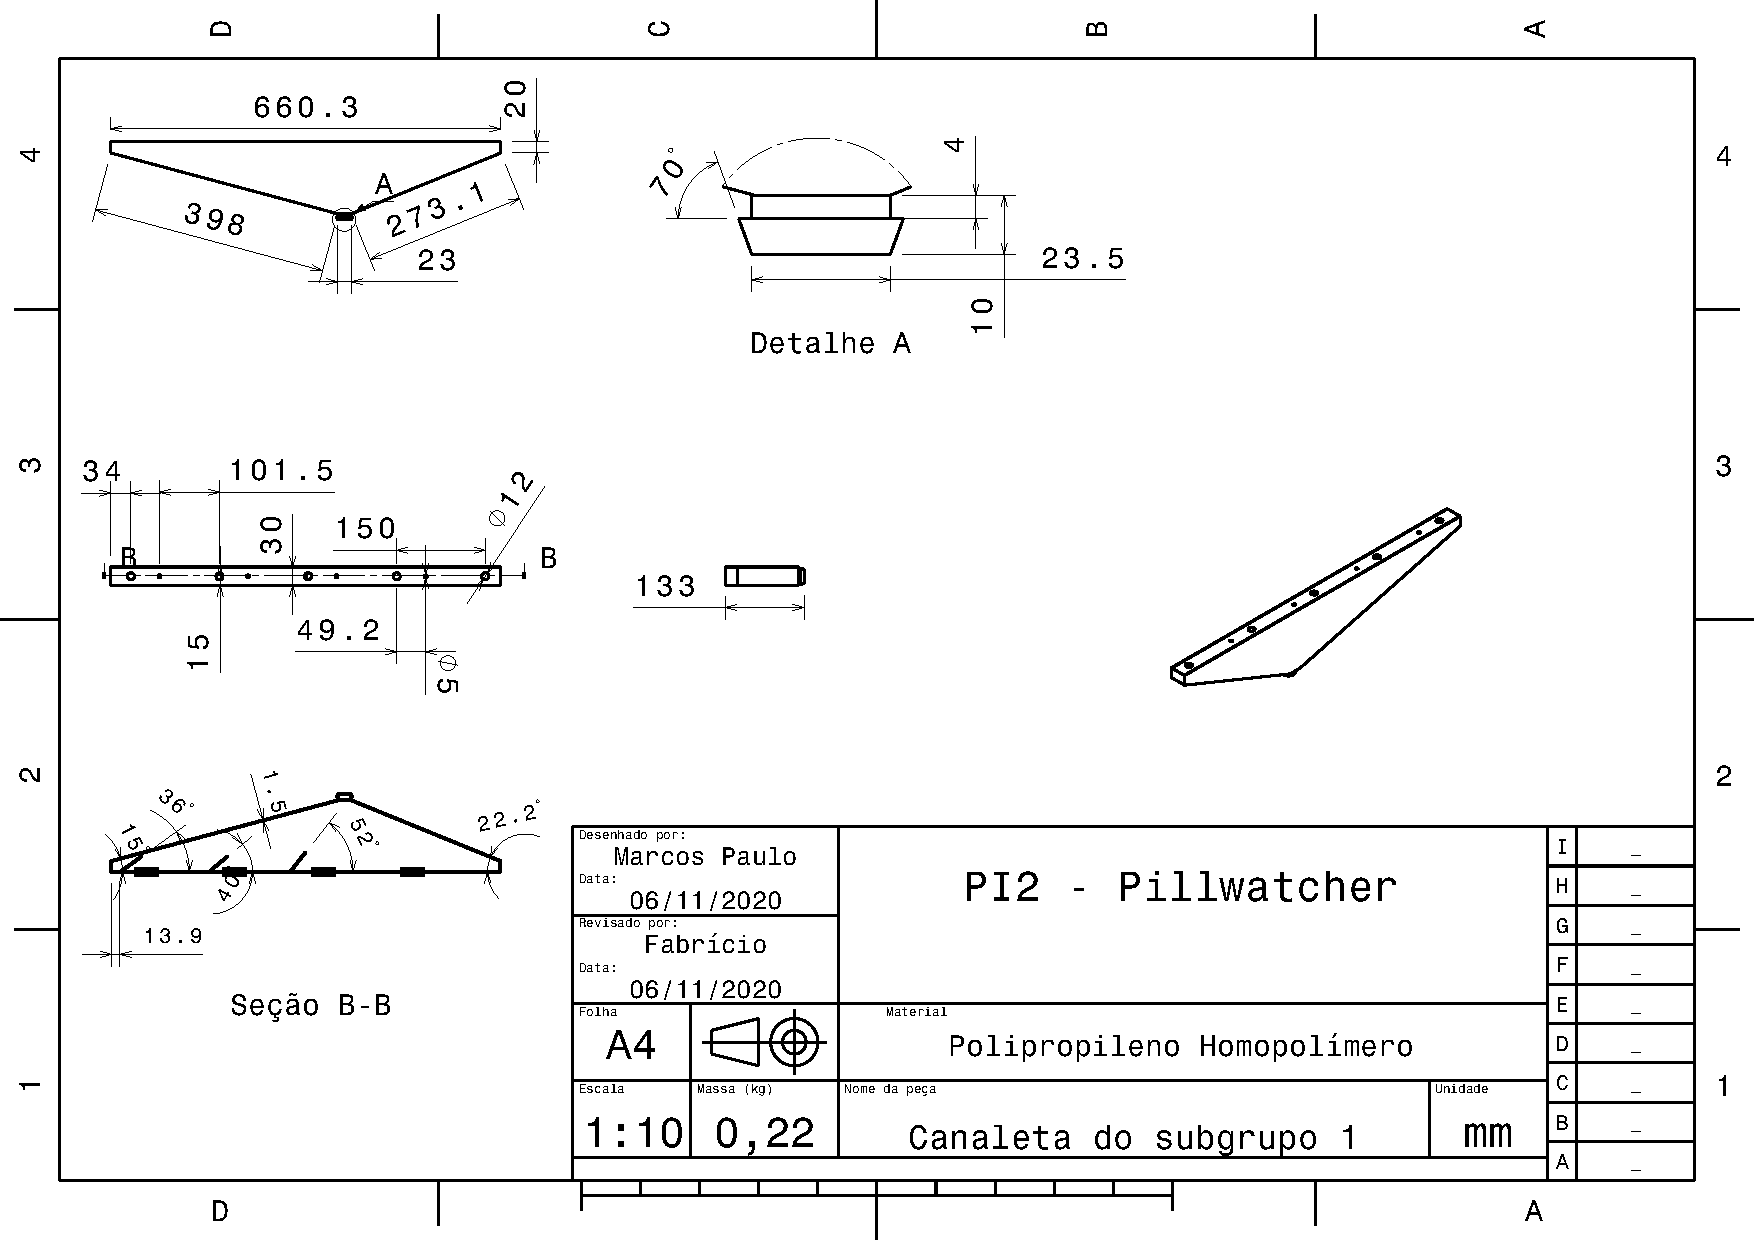
\includegraphics[width=0.9\textwidth]{figuras/estrutura/Desenhos/Canaleta_S1.pdf}
    \caption{Desenho técnico da Canaleta do Subgrupo 1 (\ref{retorno_zonadetransição})}
    \label{fig:canaletaS1}
\end{figure}

\begin{figure}[H]
    \centering
    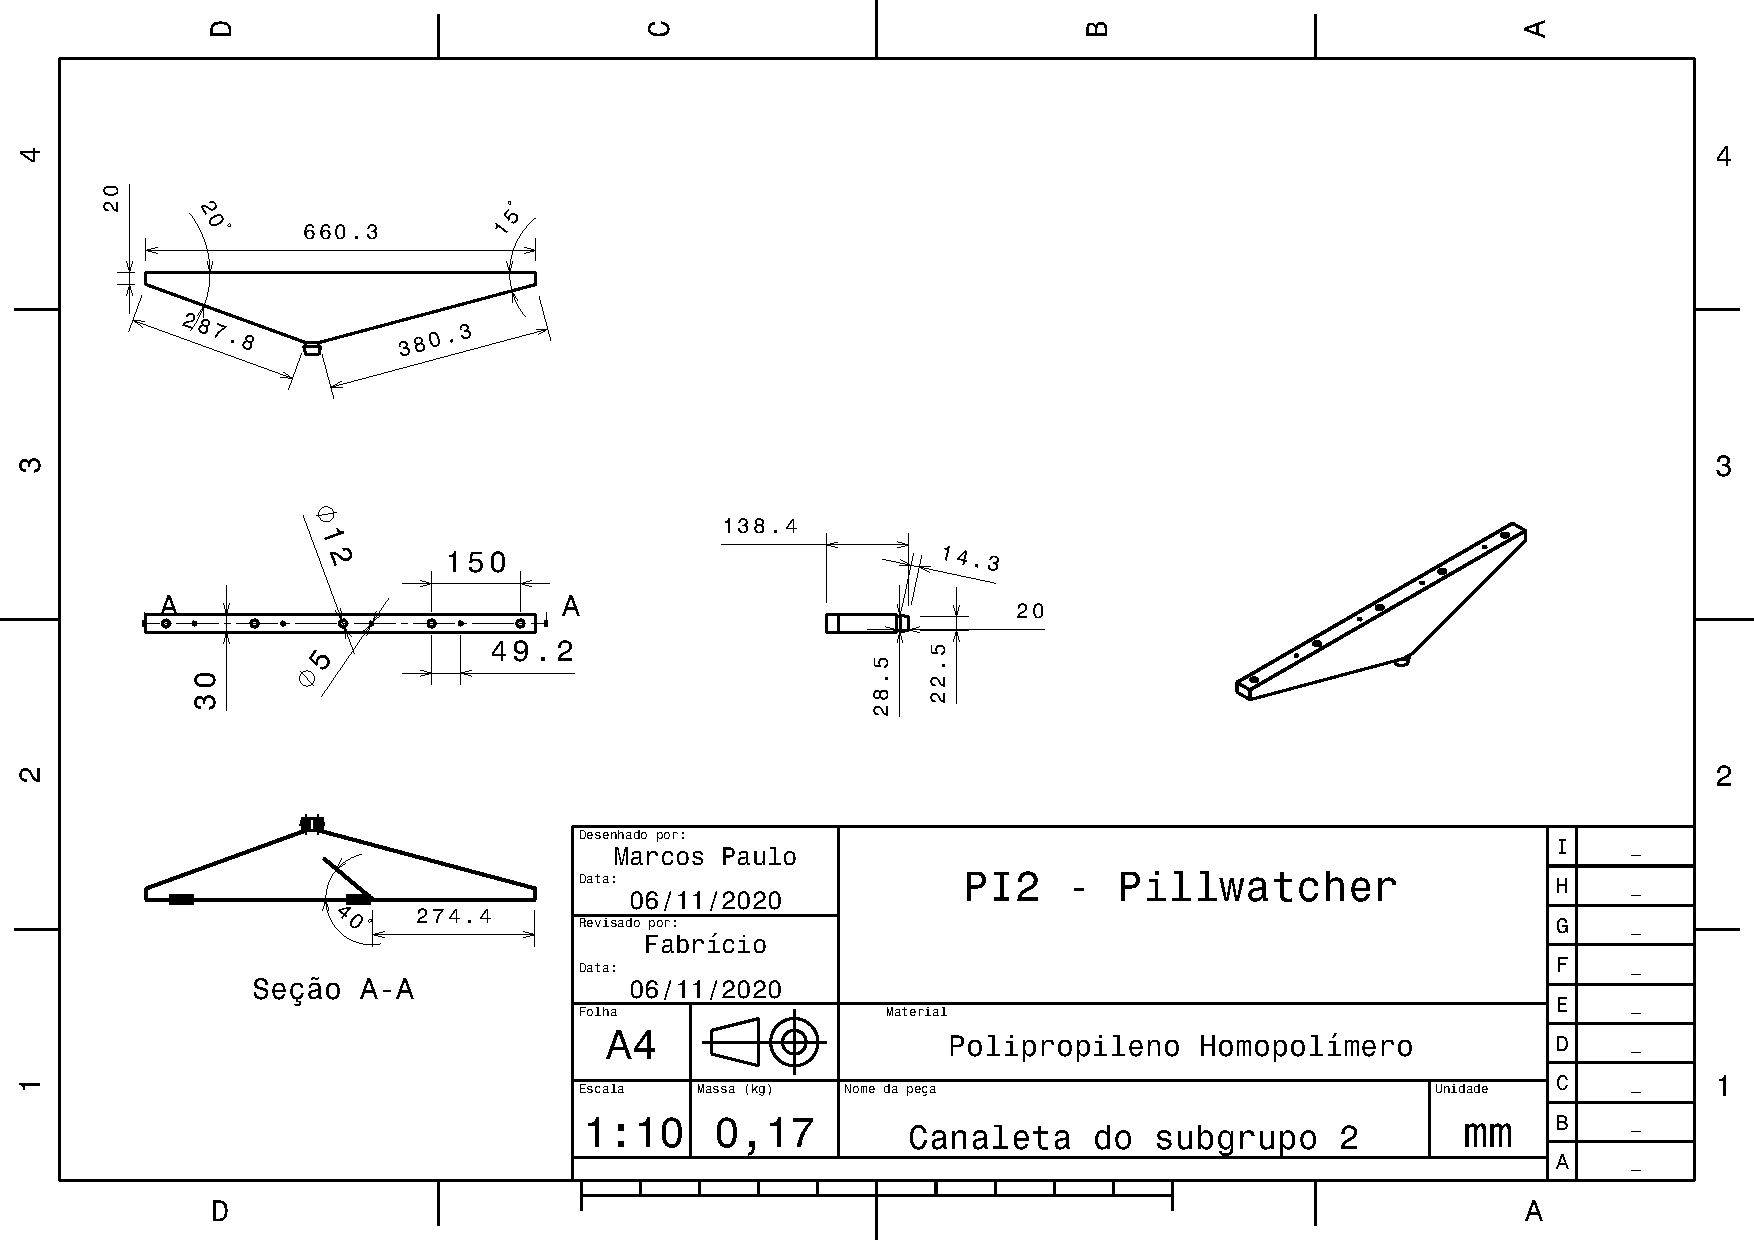
\includegraphics[width=0.9\textwidth]{figuras/estrutura/Desenhos/Canaleta_S2.pdf}
    \caption{Desenho técnico da Canaleta do Subgrupo 2 (\ref{retorno_zonadetransição})}
    \label{fig:canaletaS2}
\end{figure}

\begin{figure}[H]
    \centering
    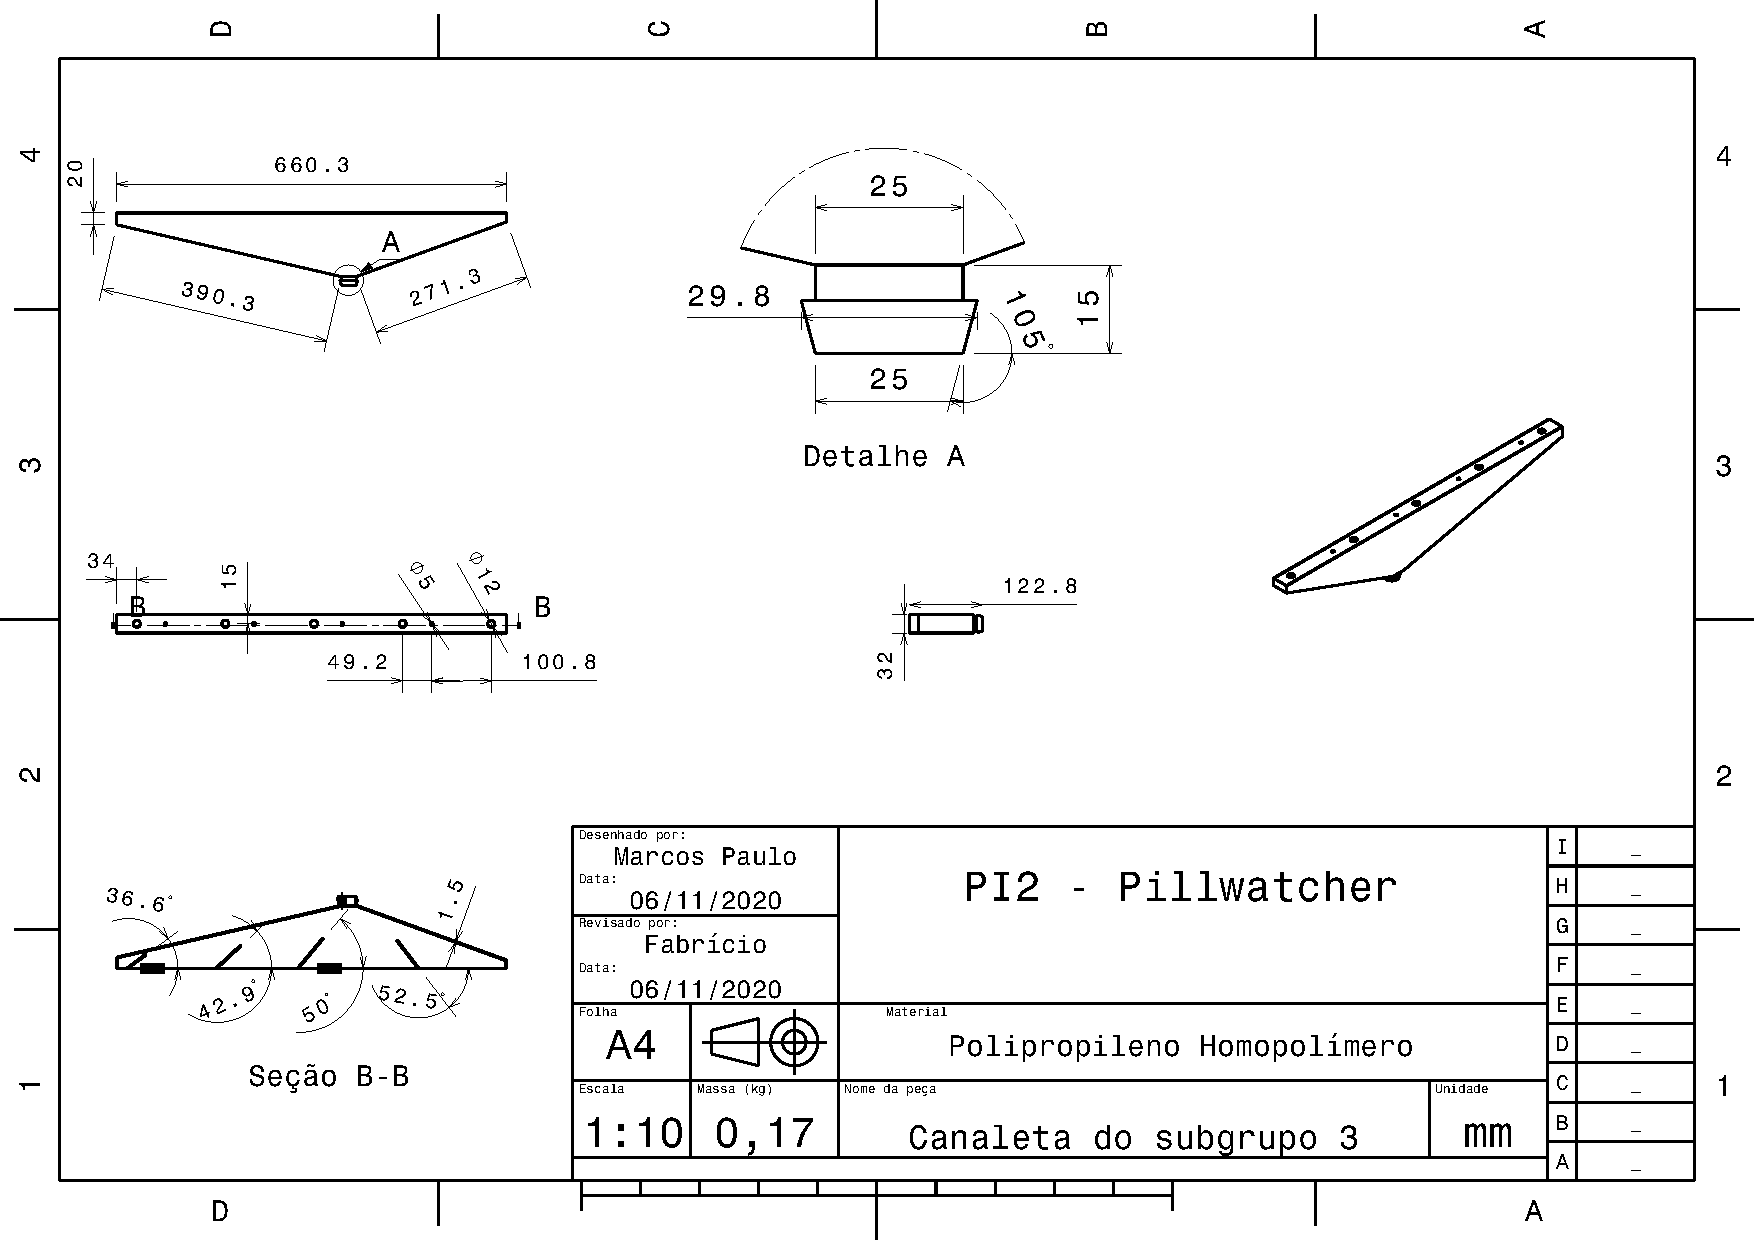
\includegraphics[width=0.9\textwidth]{figuras/estrutura/Desenhos/Canaleta_S3.pdf}
    \caption{Desenho técnico da Canaleta do Subgrupo 3 (\ref{retorno_zonadetransição})}
    \label{fig:canaletaS3}
\end{figure}

\begin{figure}[H]
    \centering
    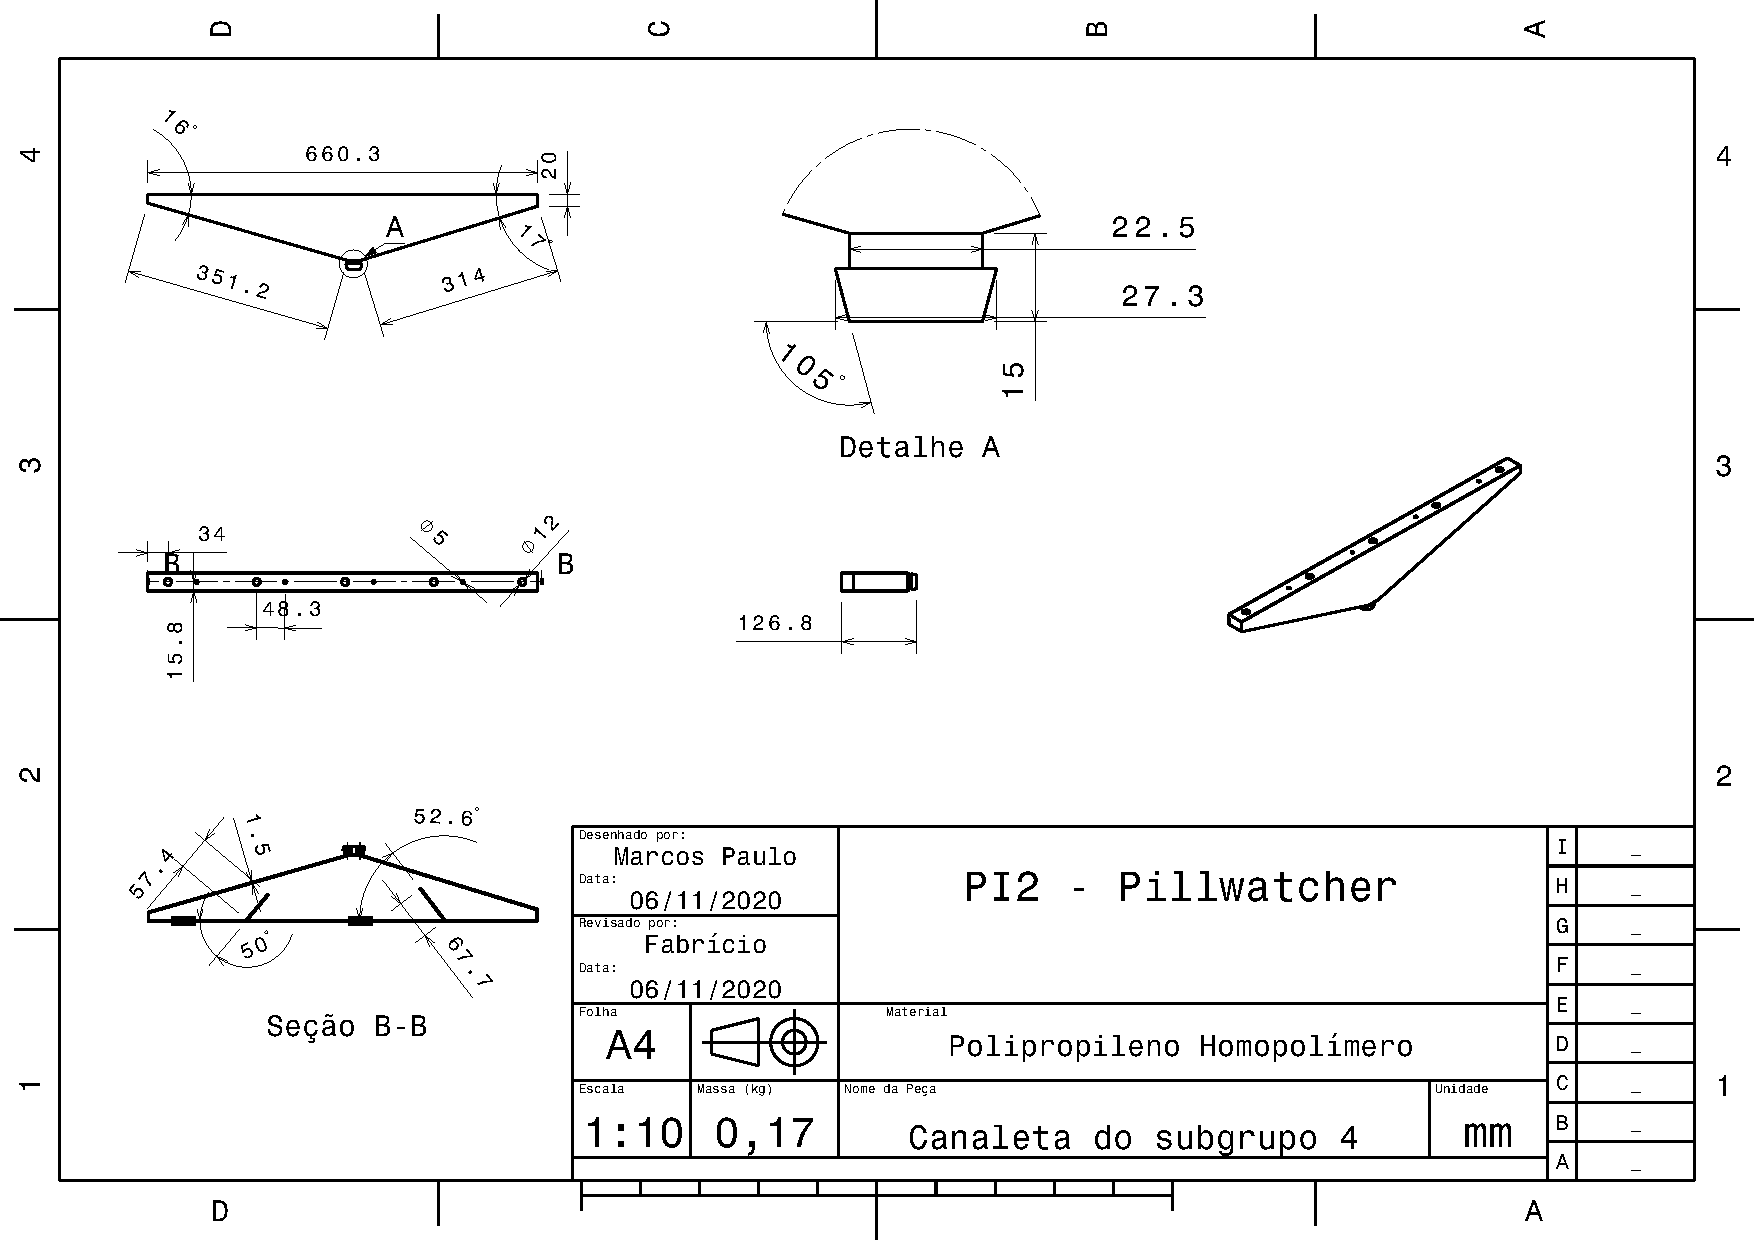
\includegraphics[width=0.9\textwidth]{figuras/estrutura/Desenhos/Canaleta_s4.pdf}
    \caption{Desenho técnico da Canaleta do Subgrupo 4 (\ref{retorno_zonadetransição})}
    \label{fig:canaletaS4}
\end{figure}

\begin{figure}[H]
    \centering
    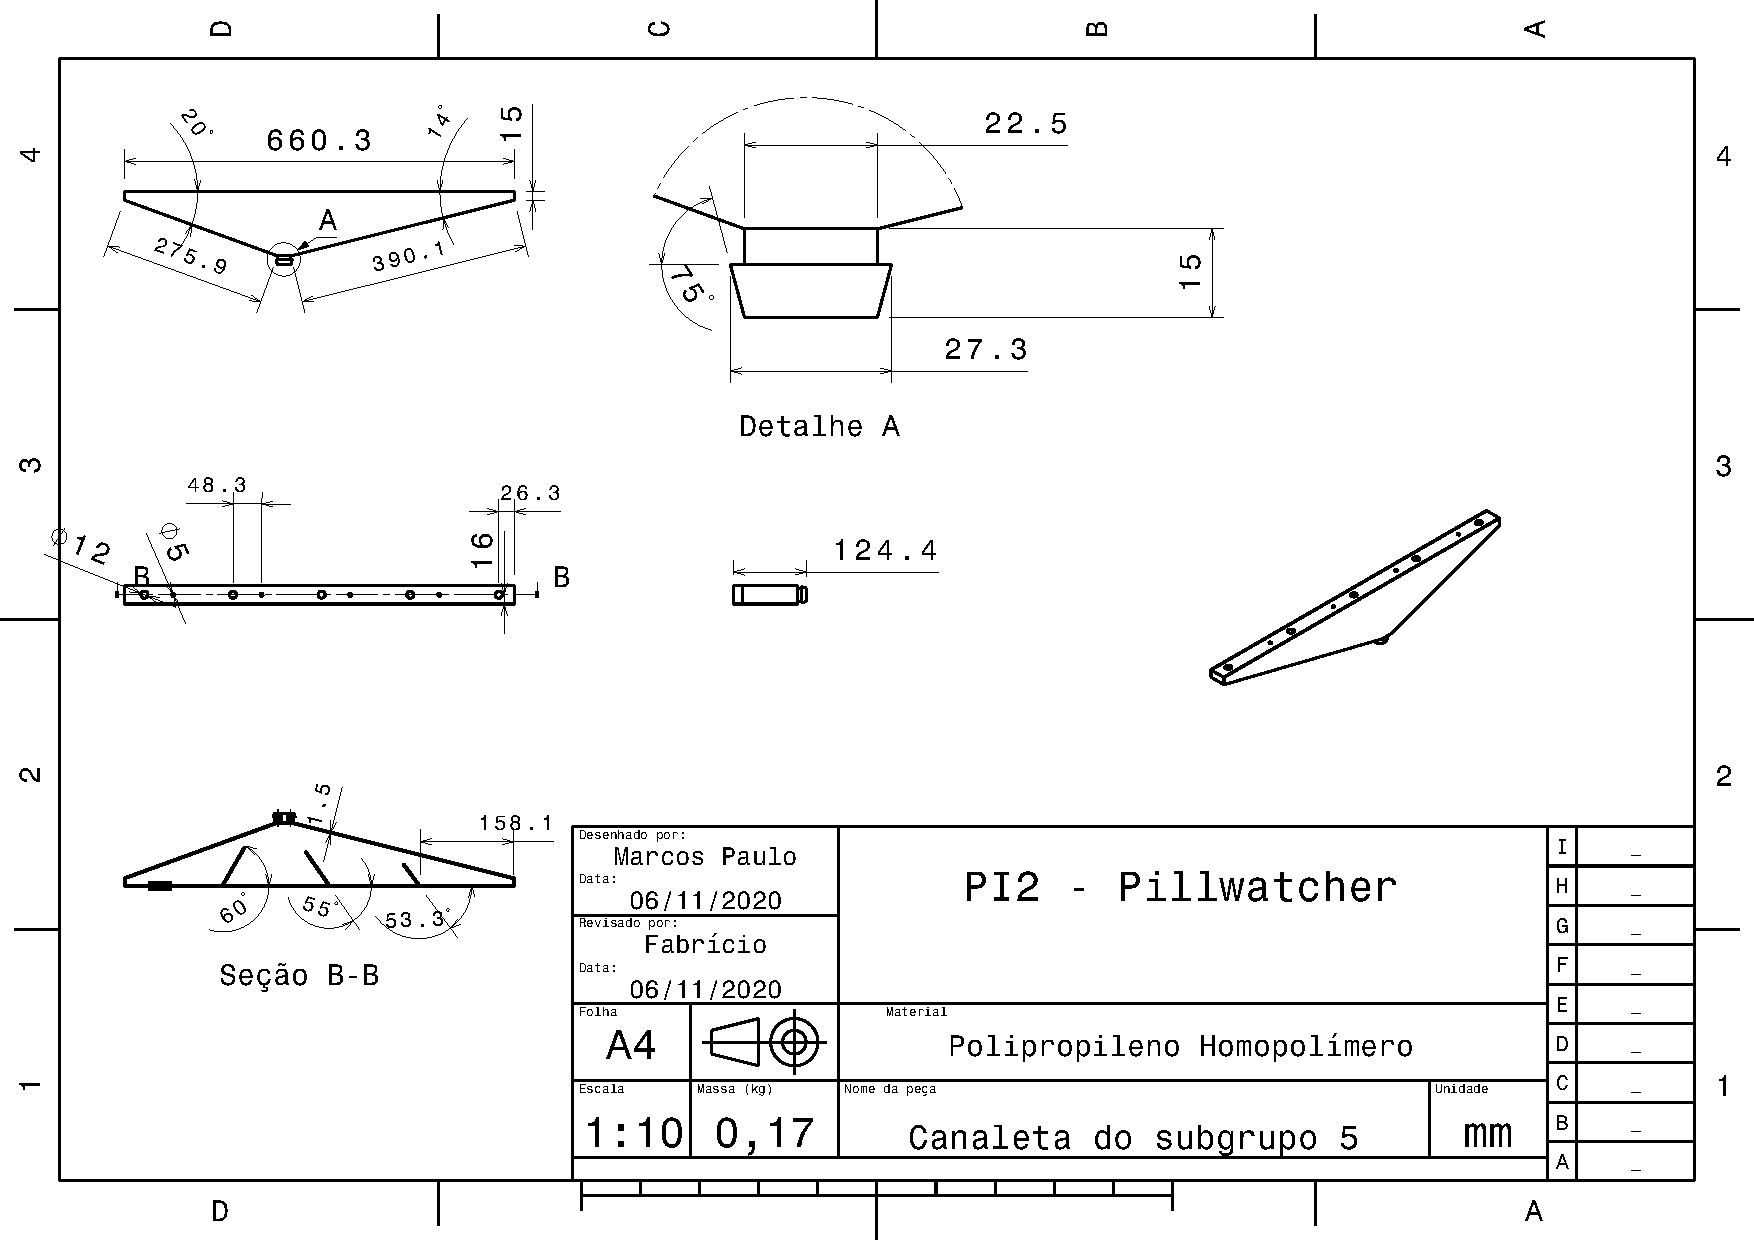
\includegraphics[width=0.9\textwidth]{figuras/estrutura/Desenhos/Canaleta_S5.pdf}
    \caption{Desenho técnico da Canaleta do Subgrupo 5 (\ref{retorno_zonadetransição})}
    \label{fig:canaletaS5}
\end{figure}

\begin{figure}[H]
    \centering
    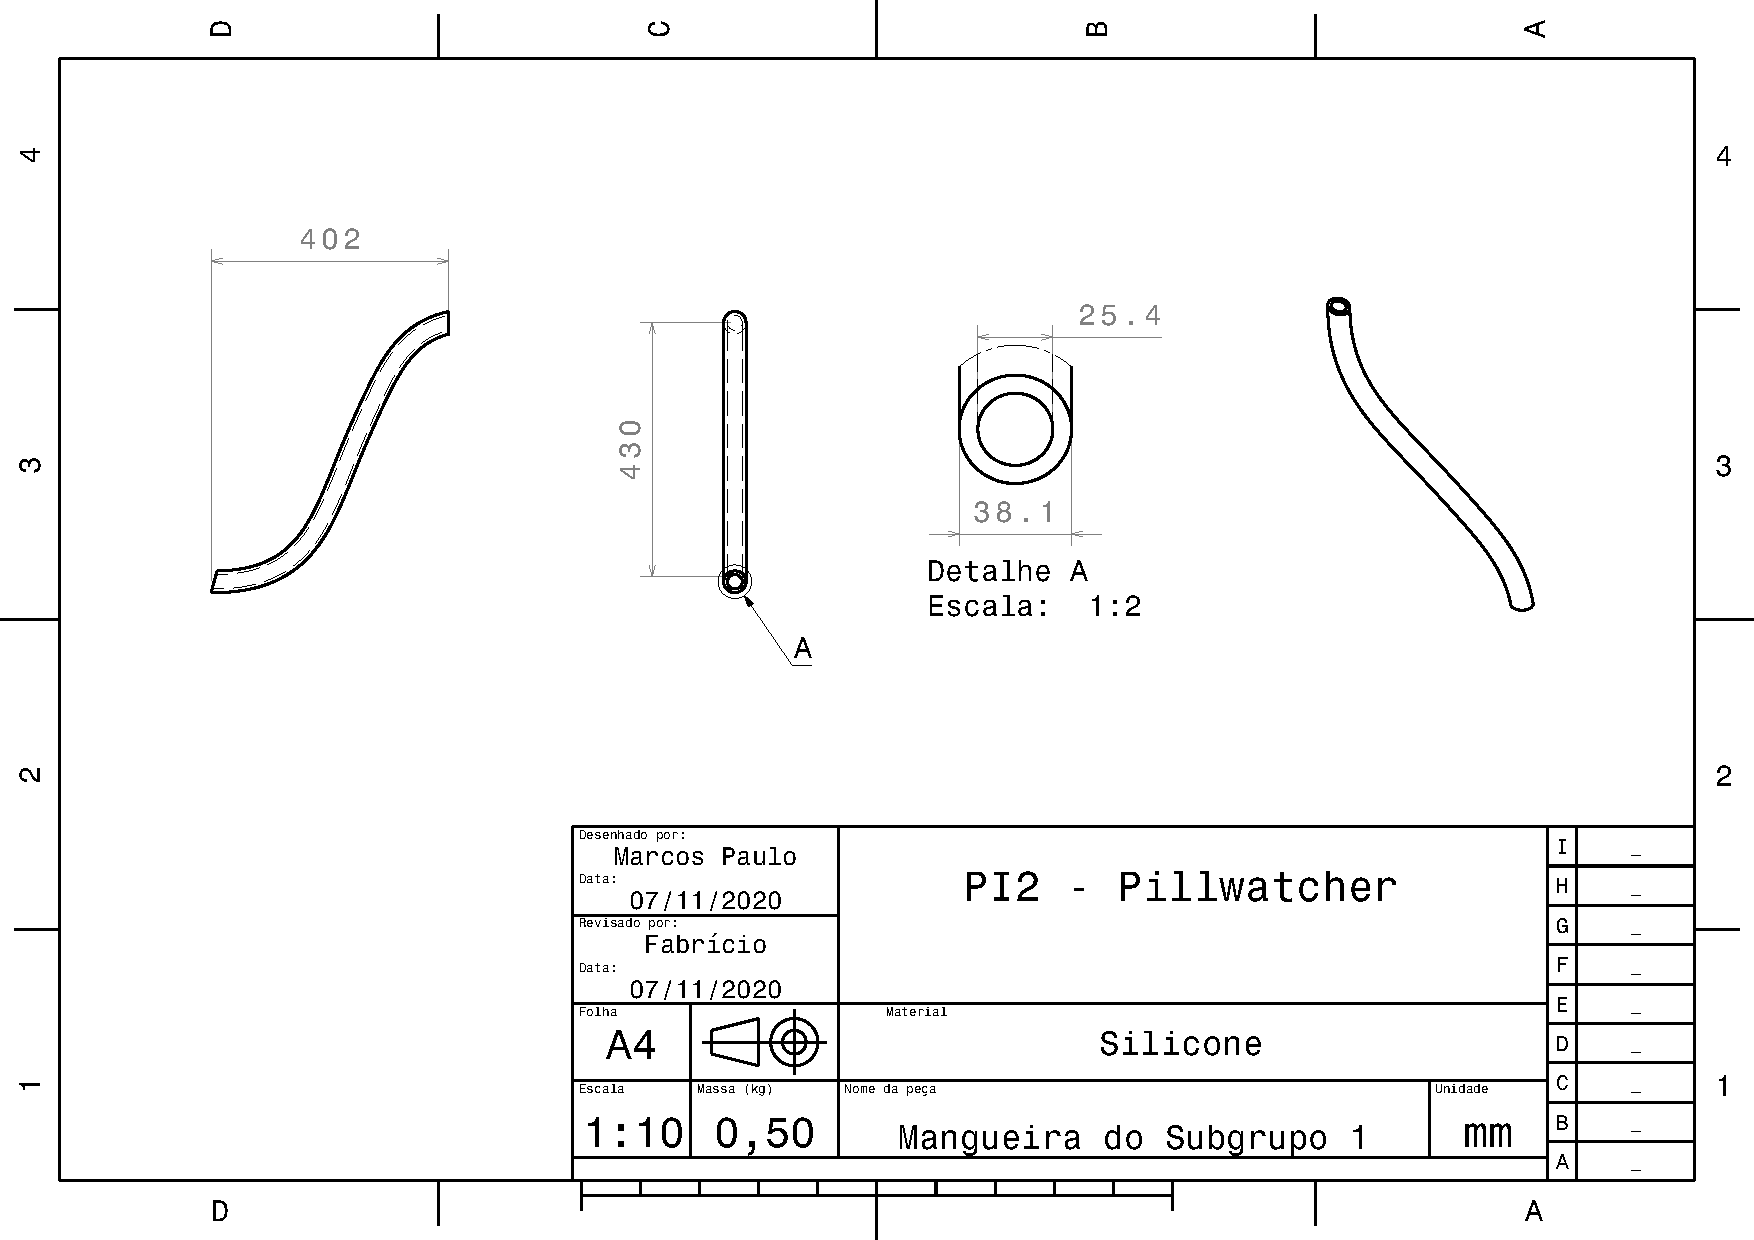
\includegraphics[width=0.9\textwidth]{figuras/estrutura/Desenhos/S1C1.pdf}
    \caption{Desenho técnico da mangueira do subgrupo 1 (\ref{retorno_mangueira})}
    \label{fig:M_S1}
\end{figure}

\begin{figure}[H]
    \centering
    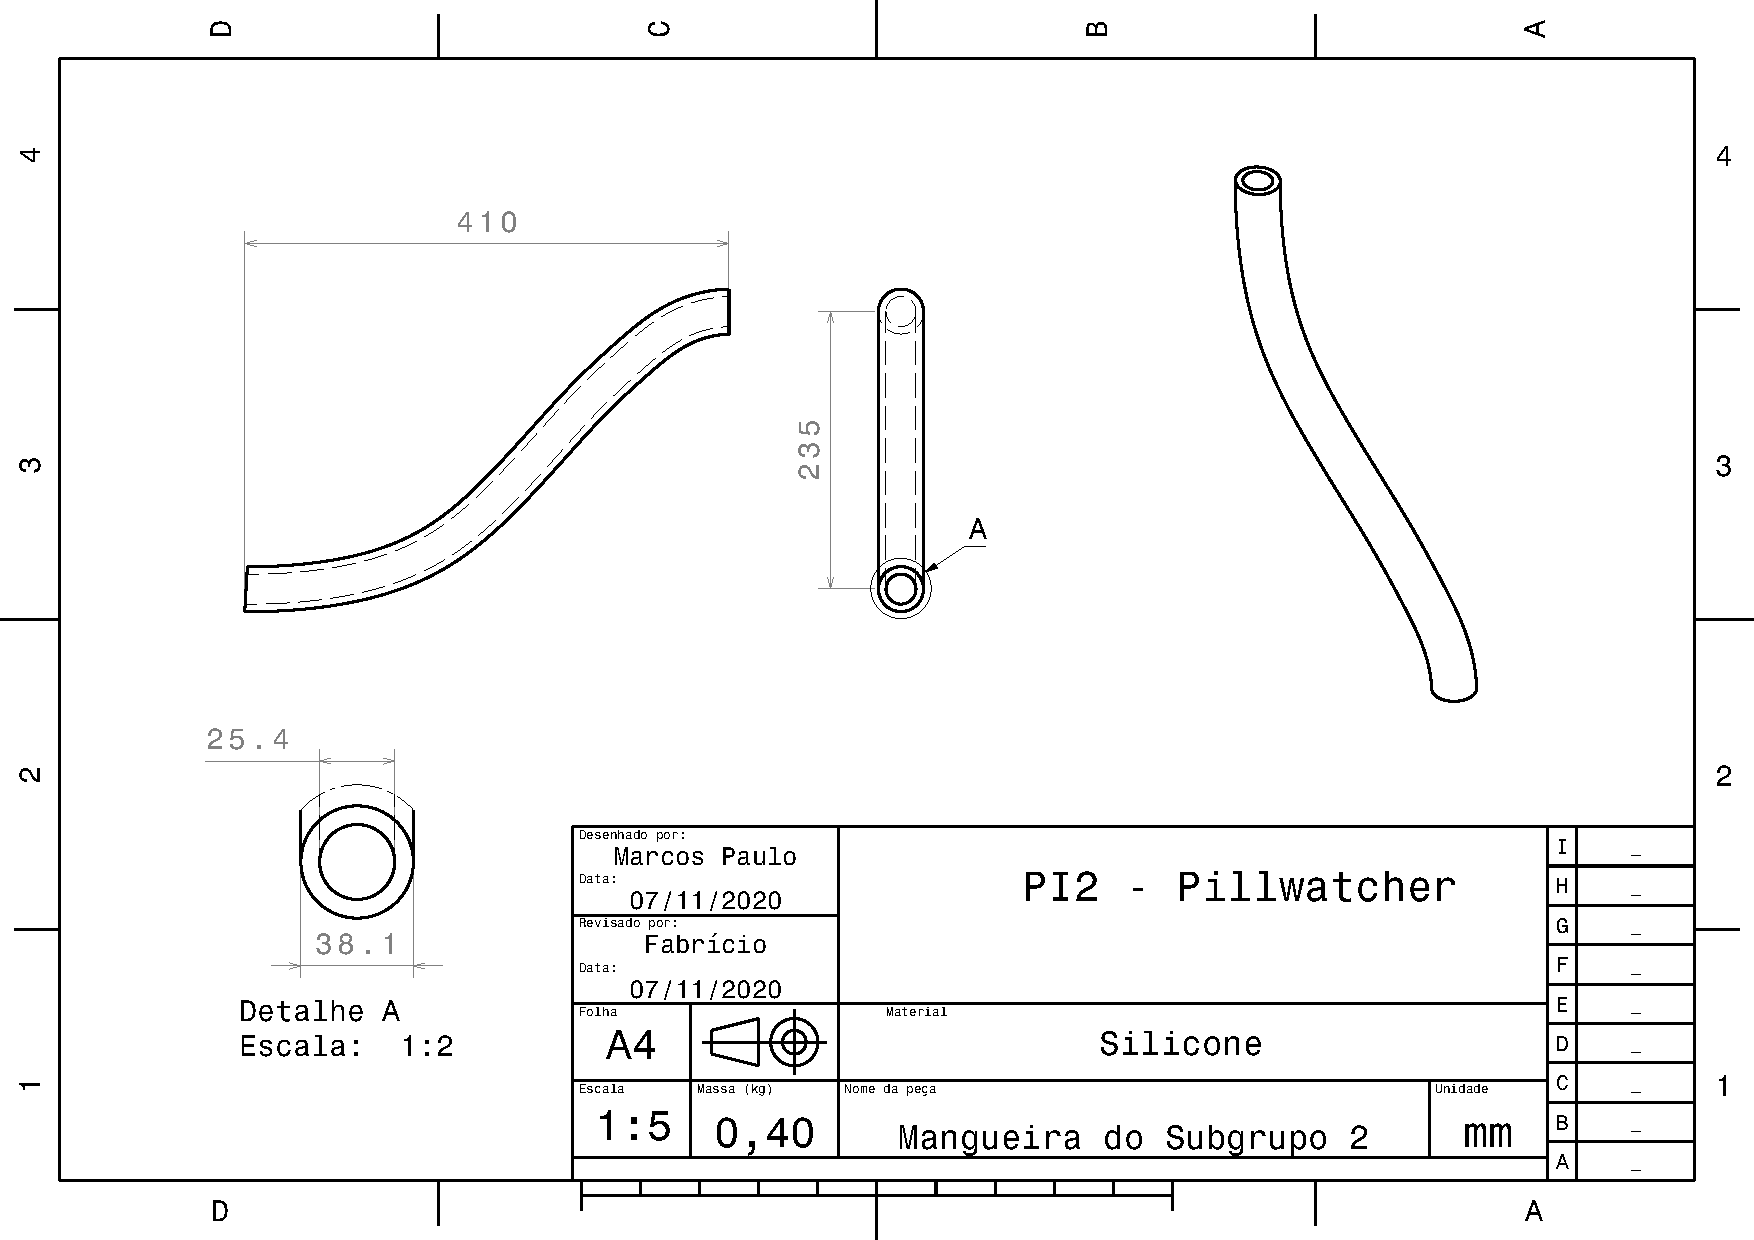
\includegraphics[width=0.9\textwidth]{figuras/estrutura/Desenhos/S1C2.pdf}
    \caption{Desenho técnico da mangueira do subgrupo 2 (\ref{retorno_mangueira})}
    \label{fig:M_S2}
\end{figure}

\begin{figure}[H]
    \centering
    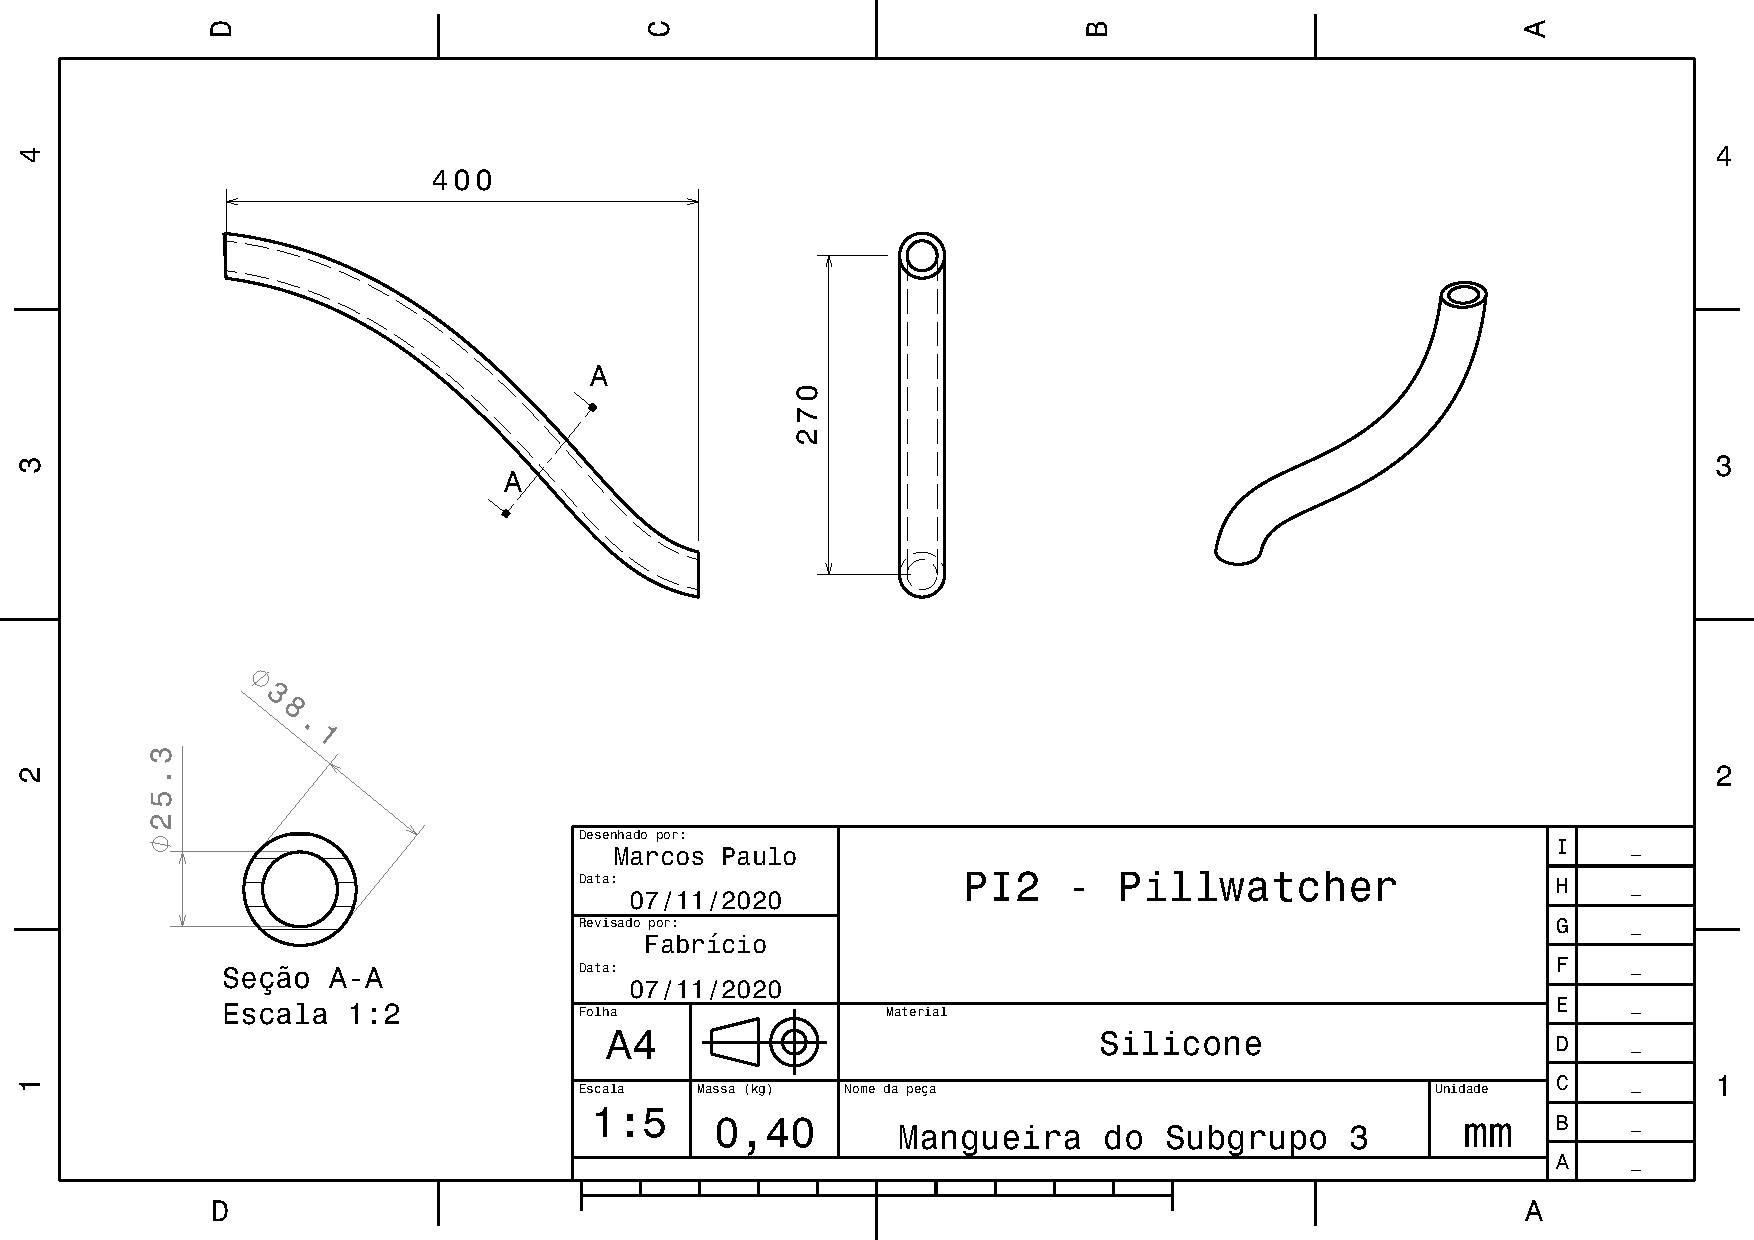
\includegraphics[width=0.9\textwidth]{figuras/estrutura/Desenhos/S1C3.pdf}
    \caption{Desenho técnico da mangueira do subgrupo 3 (\ref{retorno_mangueira})}
    \label{fig:M_S3}
\end{figure}

\begin{figure}[H]
    \centering
    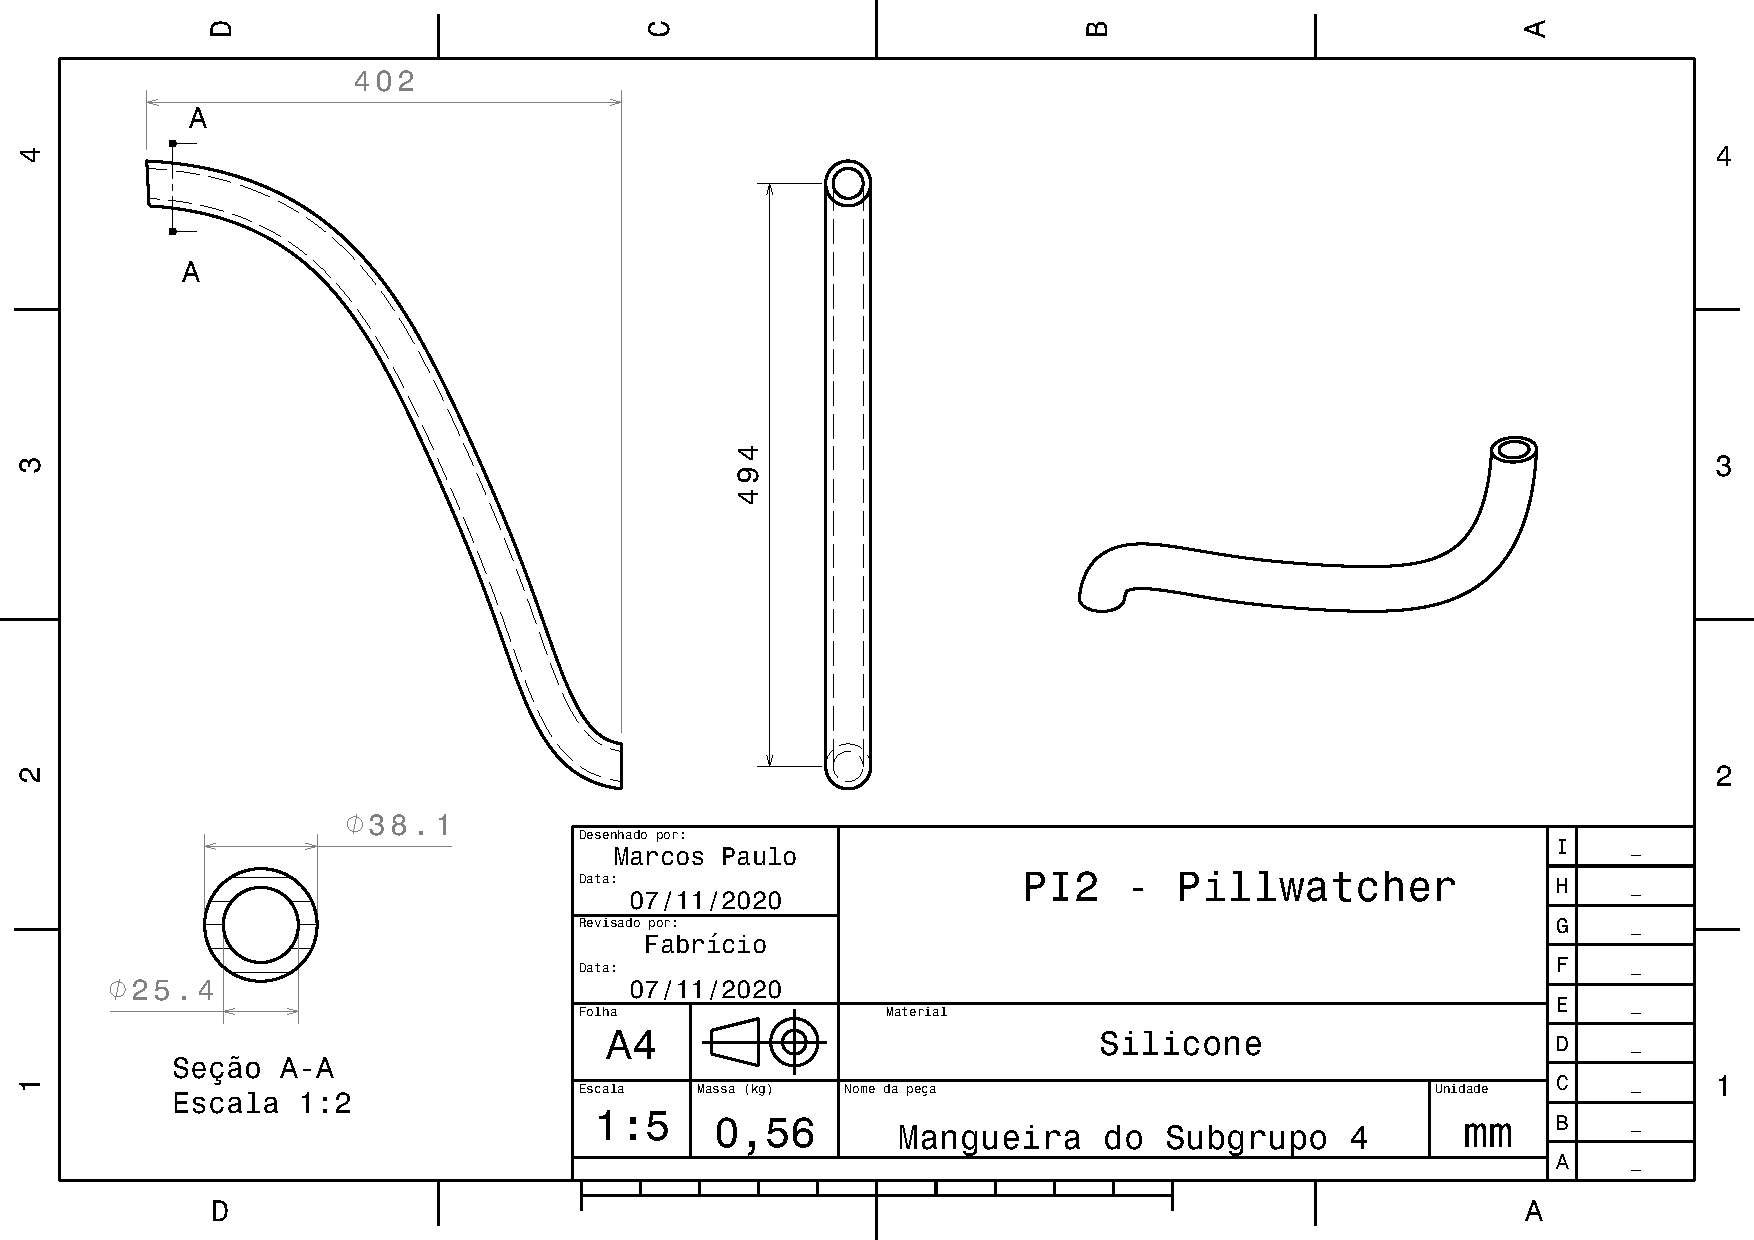
\includegraphics[width=0.9\textwidth]{figuras/estrutura/Desenhos/S1C4.pdf}
    \caption{Desenho técnico da mangueira do subgrupo 4 (\ref{retorno_mangueira})}
    \label{fig:M_S4}
\end{figure}

\begin{figure}[H]
    \centering
    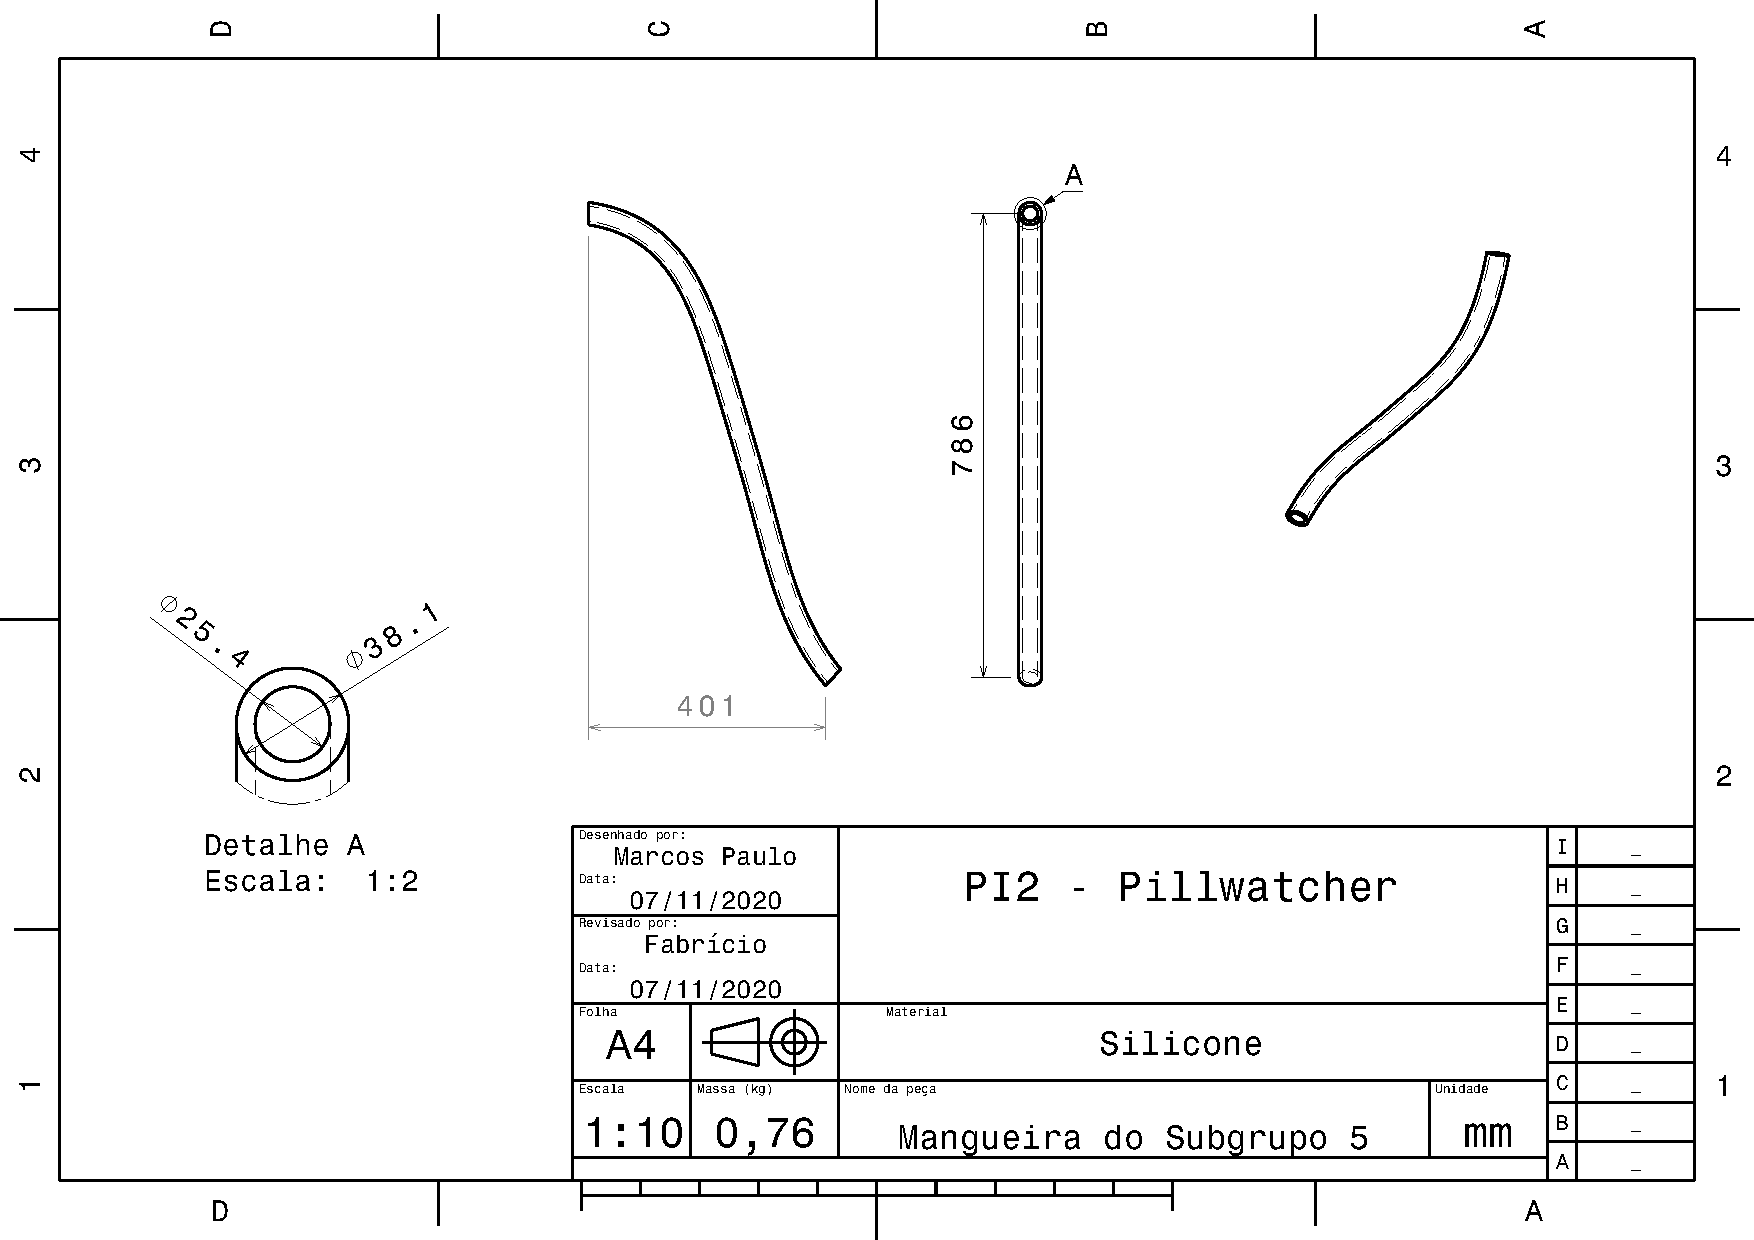
\includegraphics[width=0.9\textwidth]{figuras/estrutura/Desenhos/S1C5.pdf}
    \caption{Desenho técnico da mangueira do subgrupo 5 (\ref{retorno_mangueira})}
    \label{fig:M_S5}
\end{figure}

\begin{figure}[H]
    \centering
    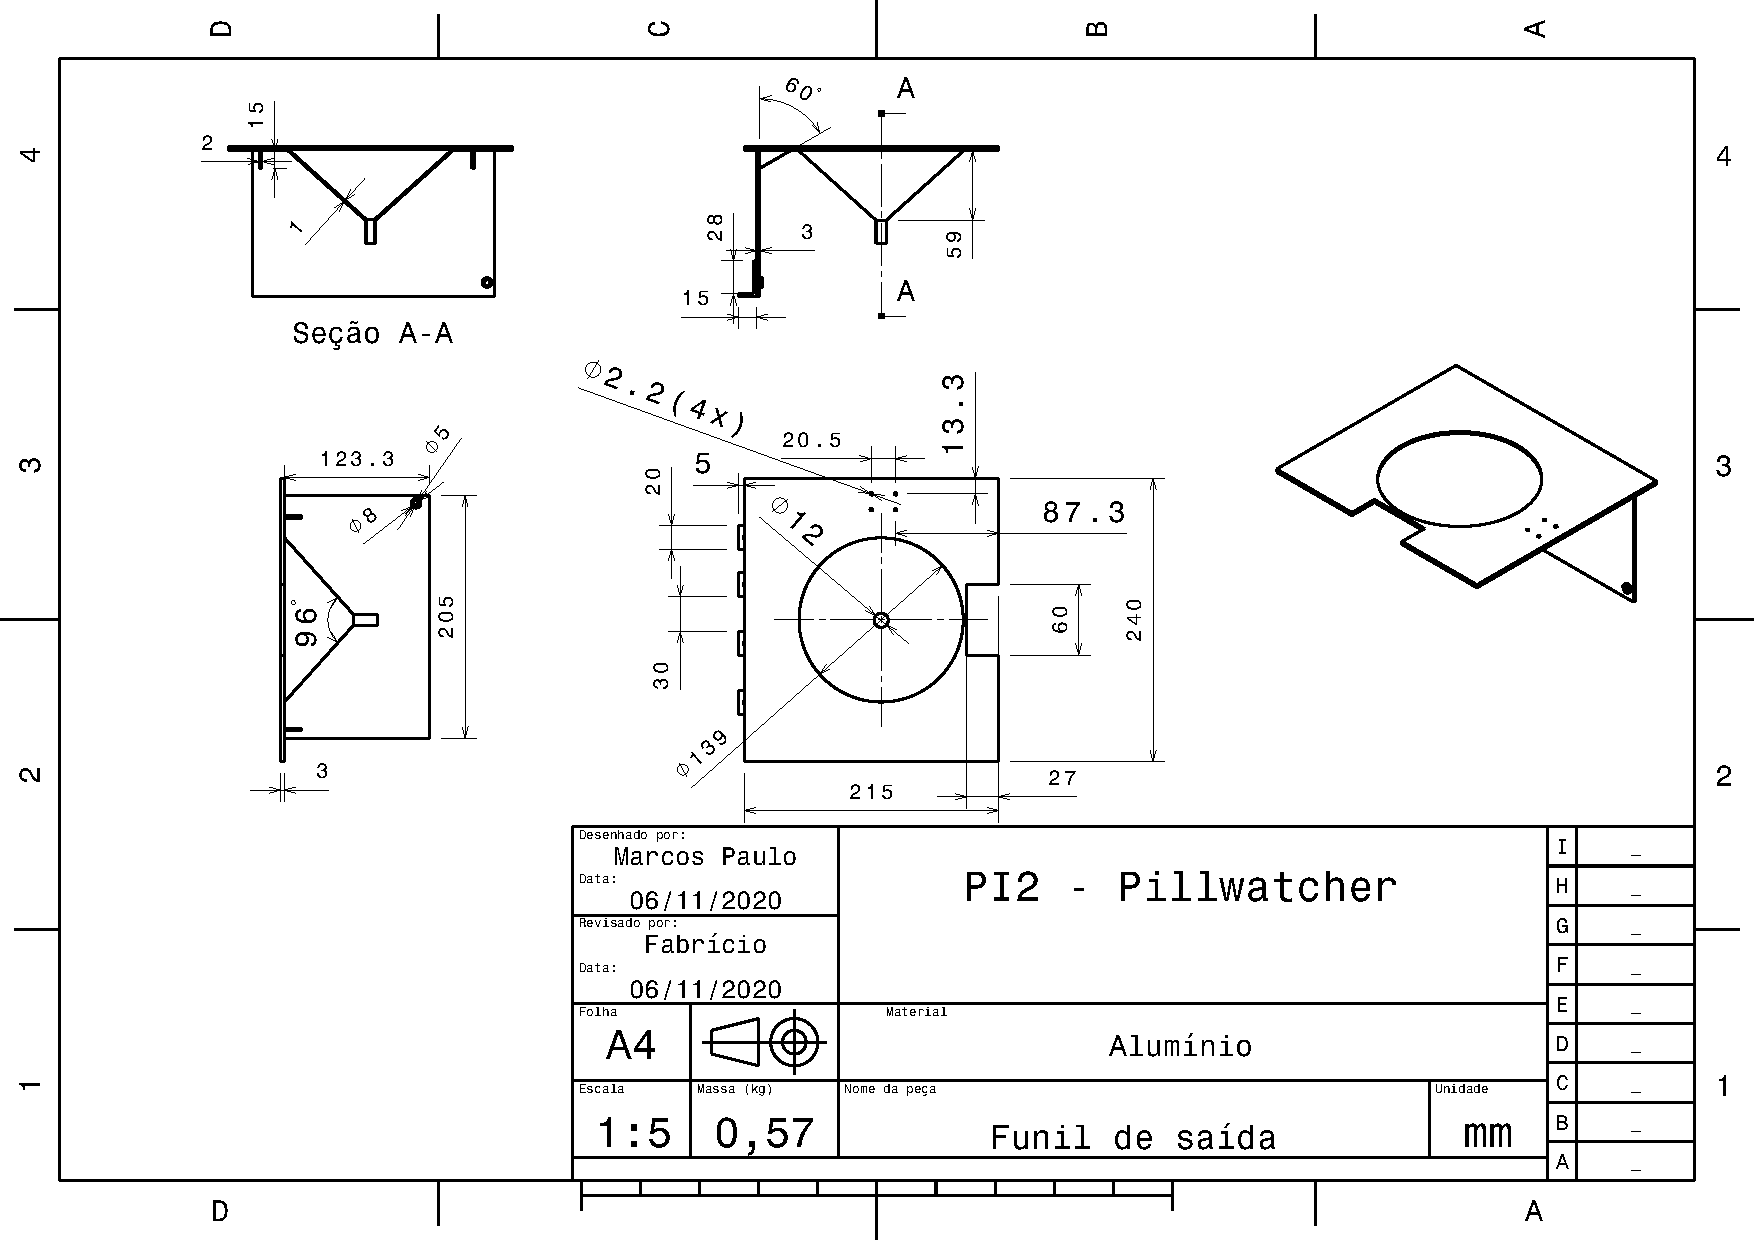
\includegraphics[width=0.9\textwidth]{figuras/estrutura/Desenhos/FunildeSaida.pdf}
    \caption{Desenho técnico do funil de saída das mangueiras (\ref{retorno_funil})}
    \label{fig:funil}
\end{figure}

\begin{figure}[H]
    \centering
    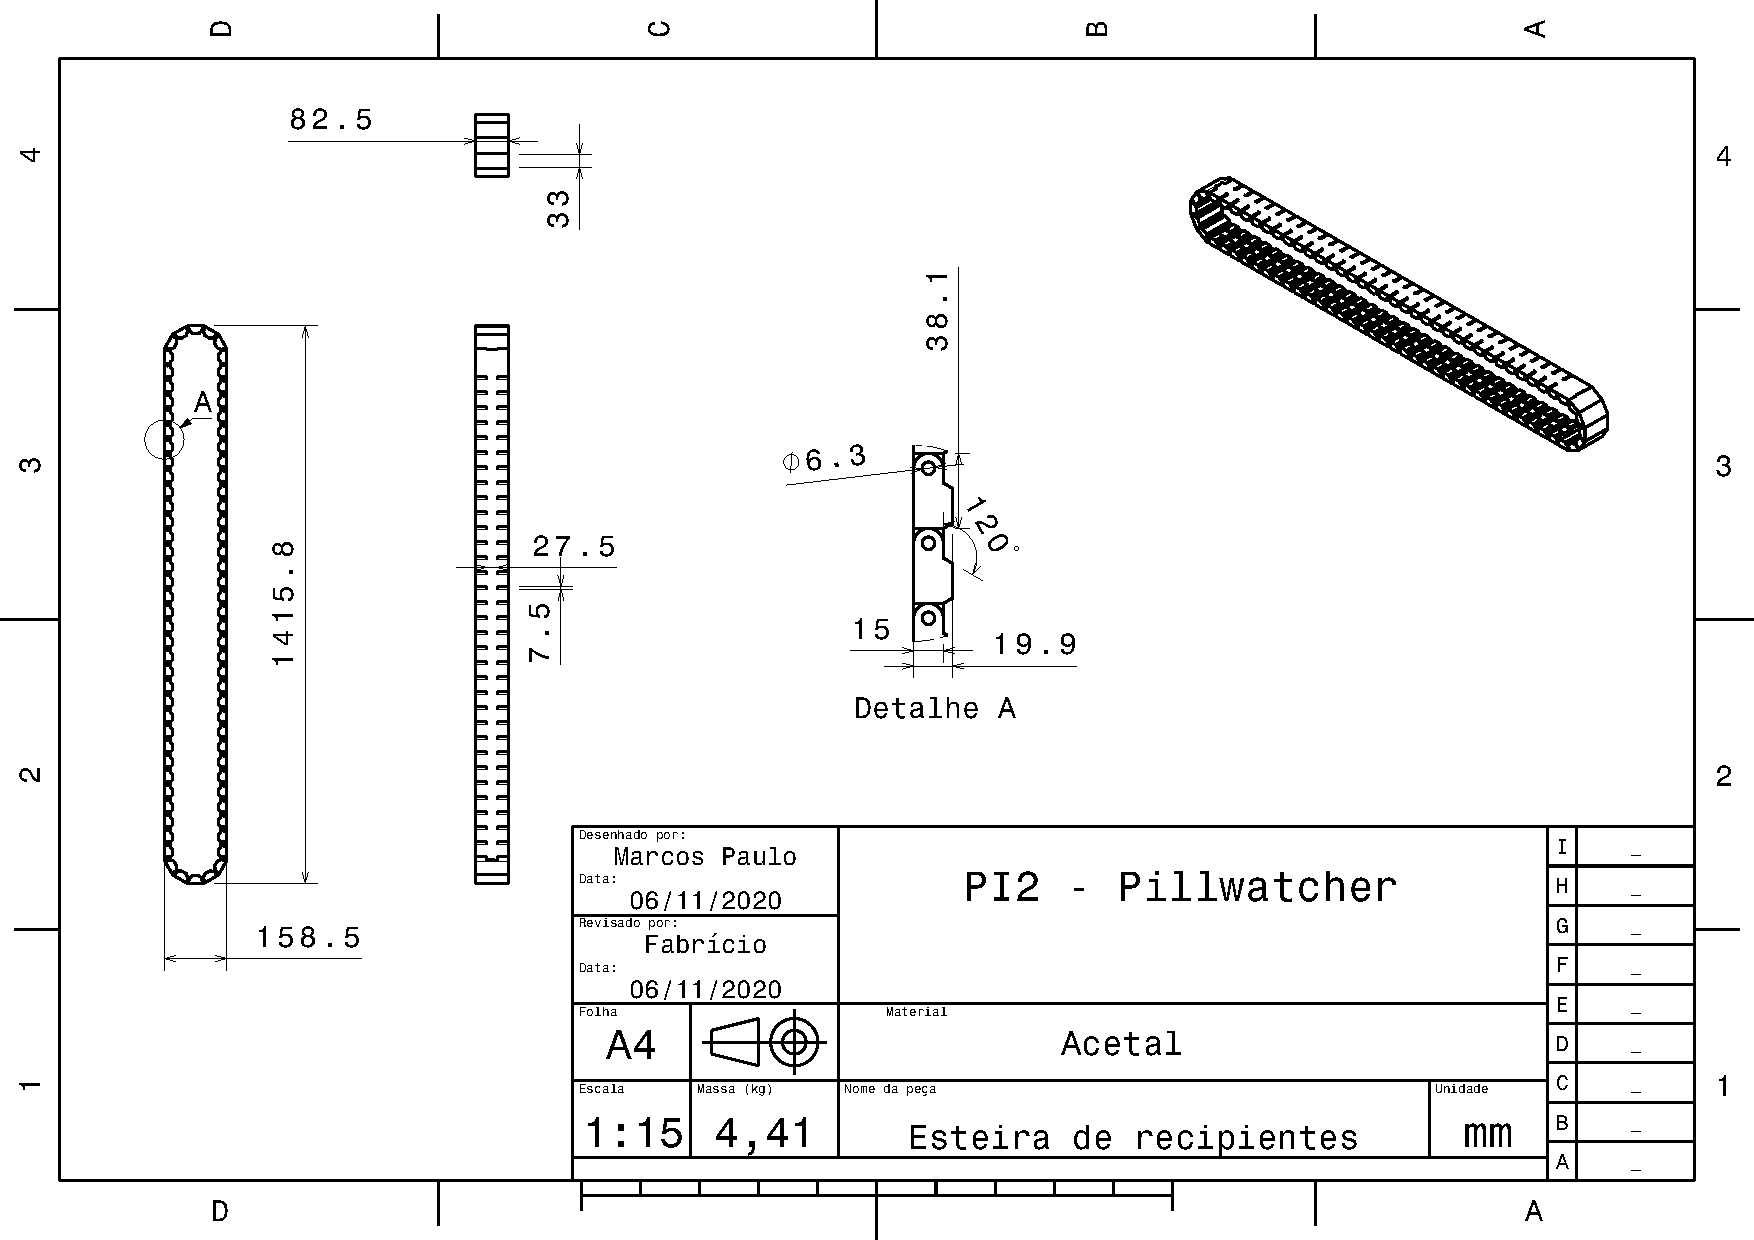
\includegraphics[width=0.9\textwidth]{figuras/estrutura/Desenhos/Esteira.pdf}
    \caption{Desenho técnico da esteira dos copos (\ref{retorno_esteira})}
    \label{fig:esteira}
\end{figure}

\begin{figure}[H]
    \centering
    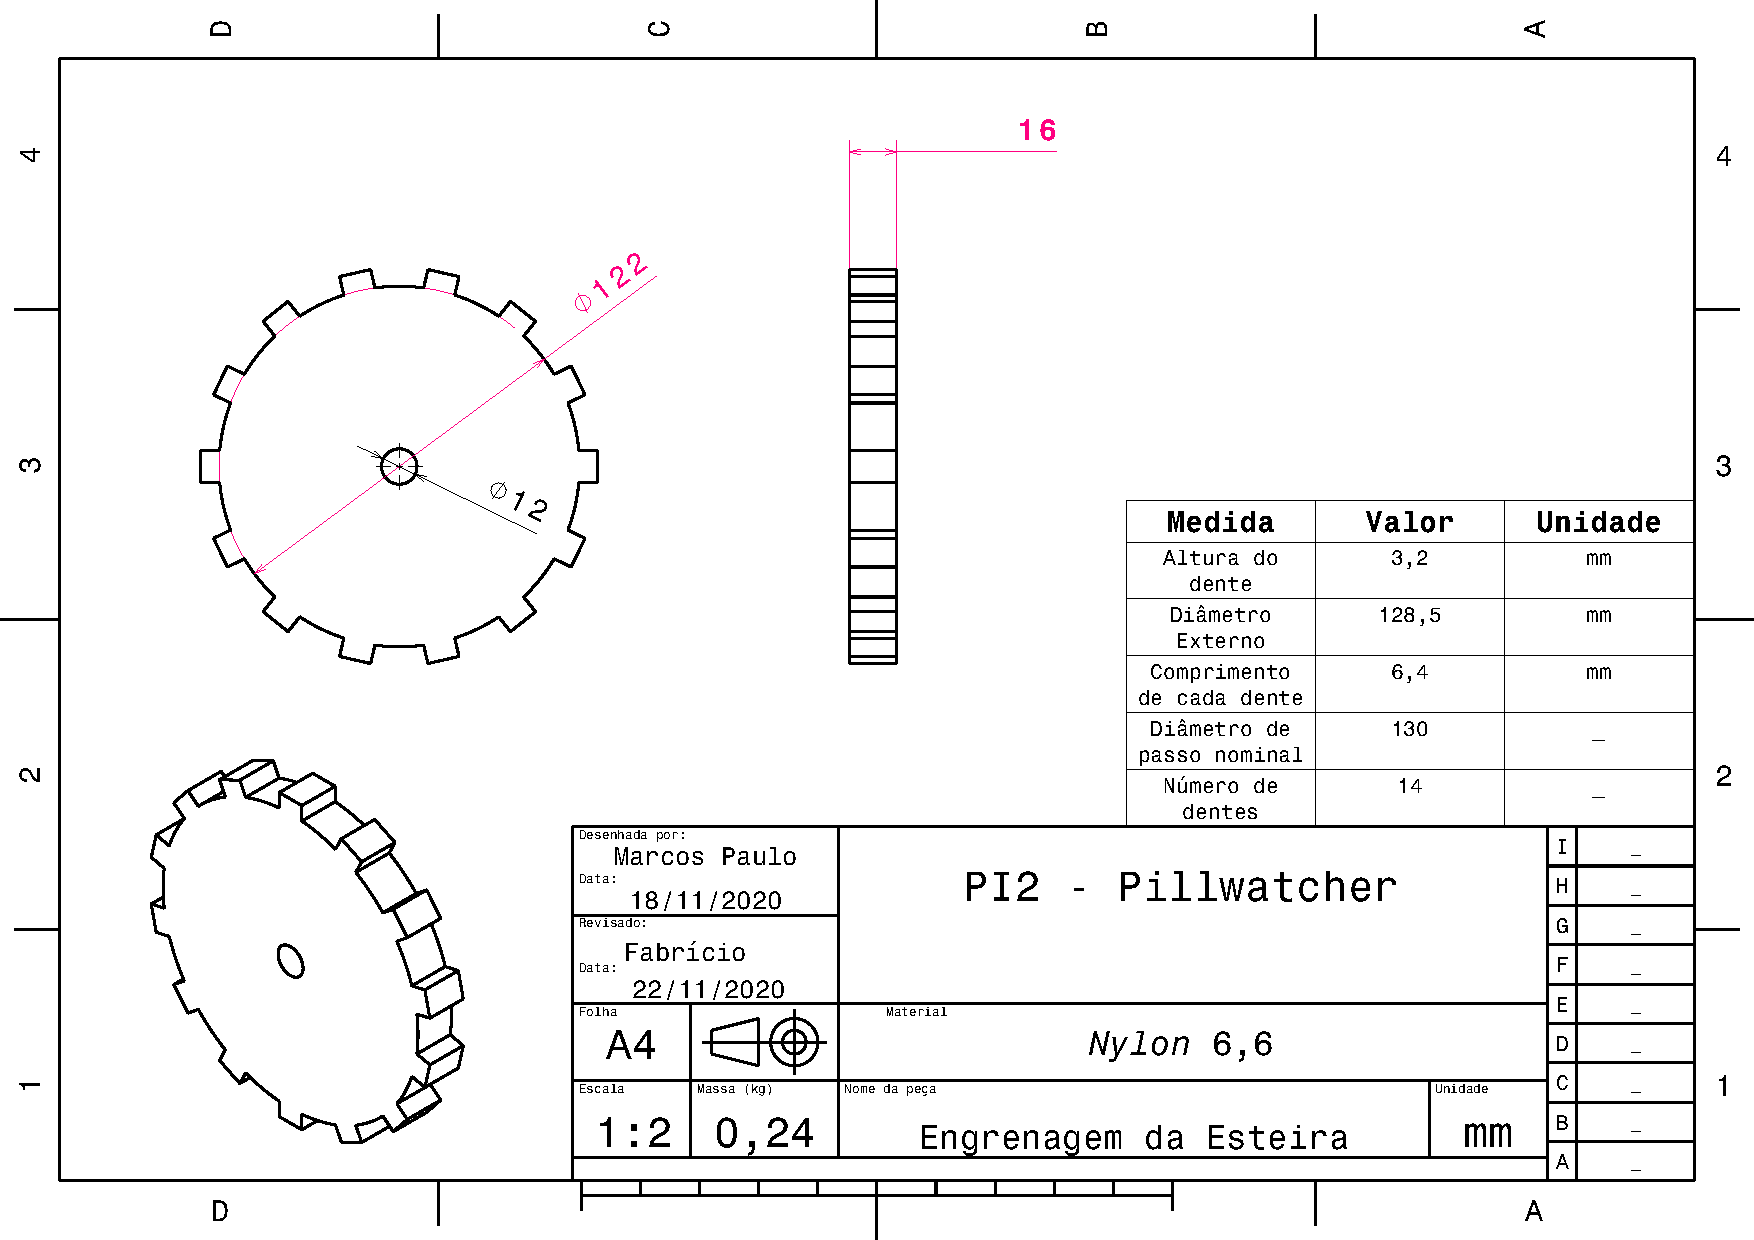
\includegraphics[width=0.9\textwidth]{figuras/estrutura/Desenhos/Engrenagem_Esteira_V2.pdf}
    \caption{Desenho técnico da engrenagem da esteira (\ref{retorno_esteira})}
    \label{fig:engrenagem_esteira}
\end{figure}

\begin{figure}[H]
    \centering
    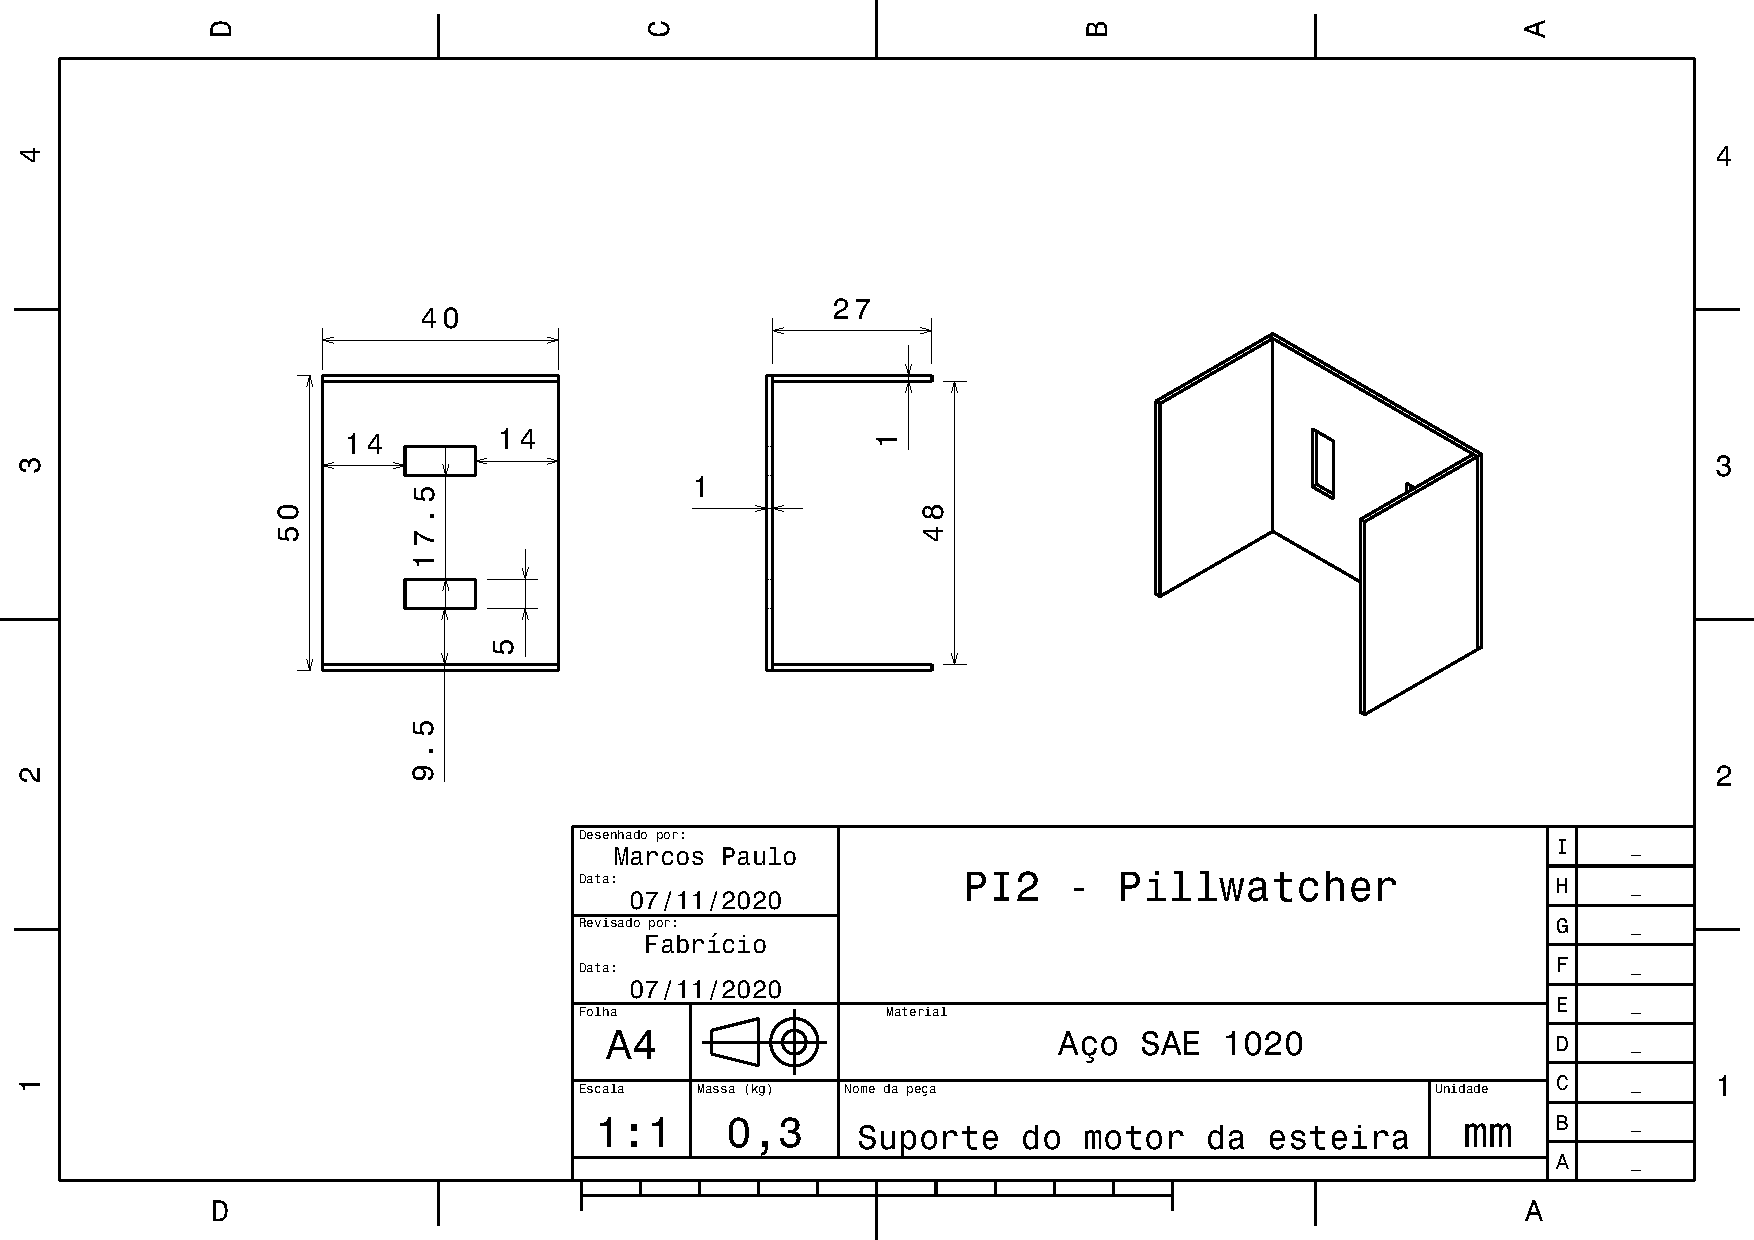
\includegraphics[width=0.9\textwidth]{figuras/estrutura/Desenhos/Suporte_MotorDC.pdf}
    \caption{Desenho técnico do suporte do motor DC da esteira (\ref{Retorno_suporte_motorDC})}
    \label{fig:supp_motordc}
\end{figure}

\begin{figure}[H]
    \centering
    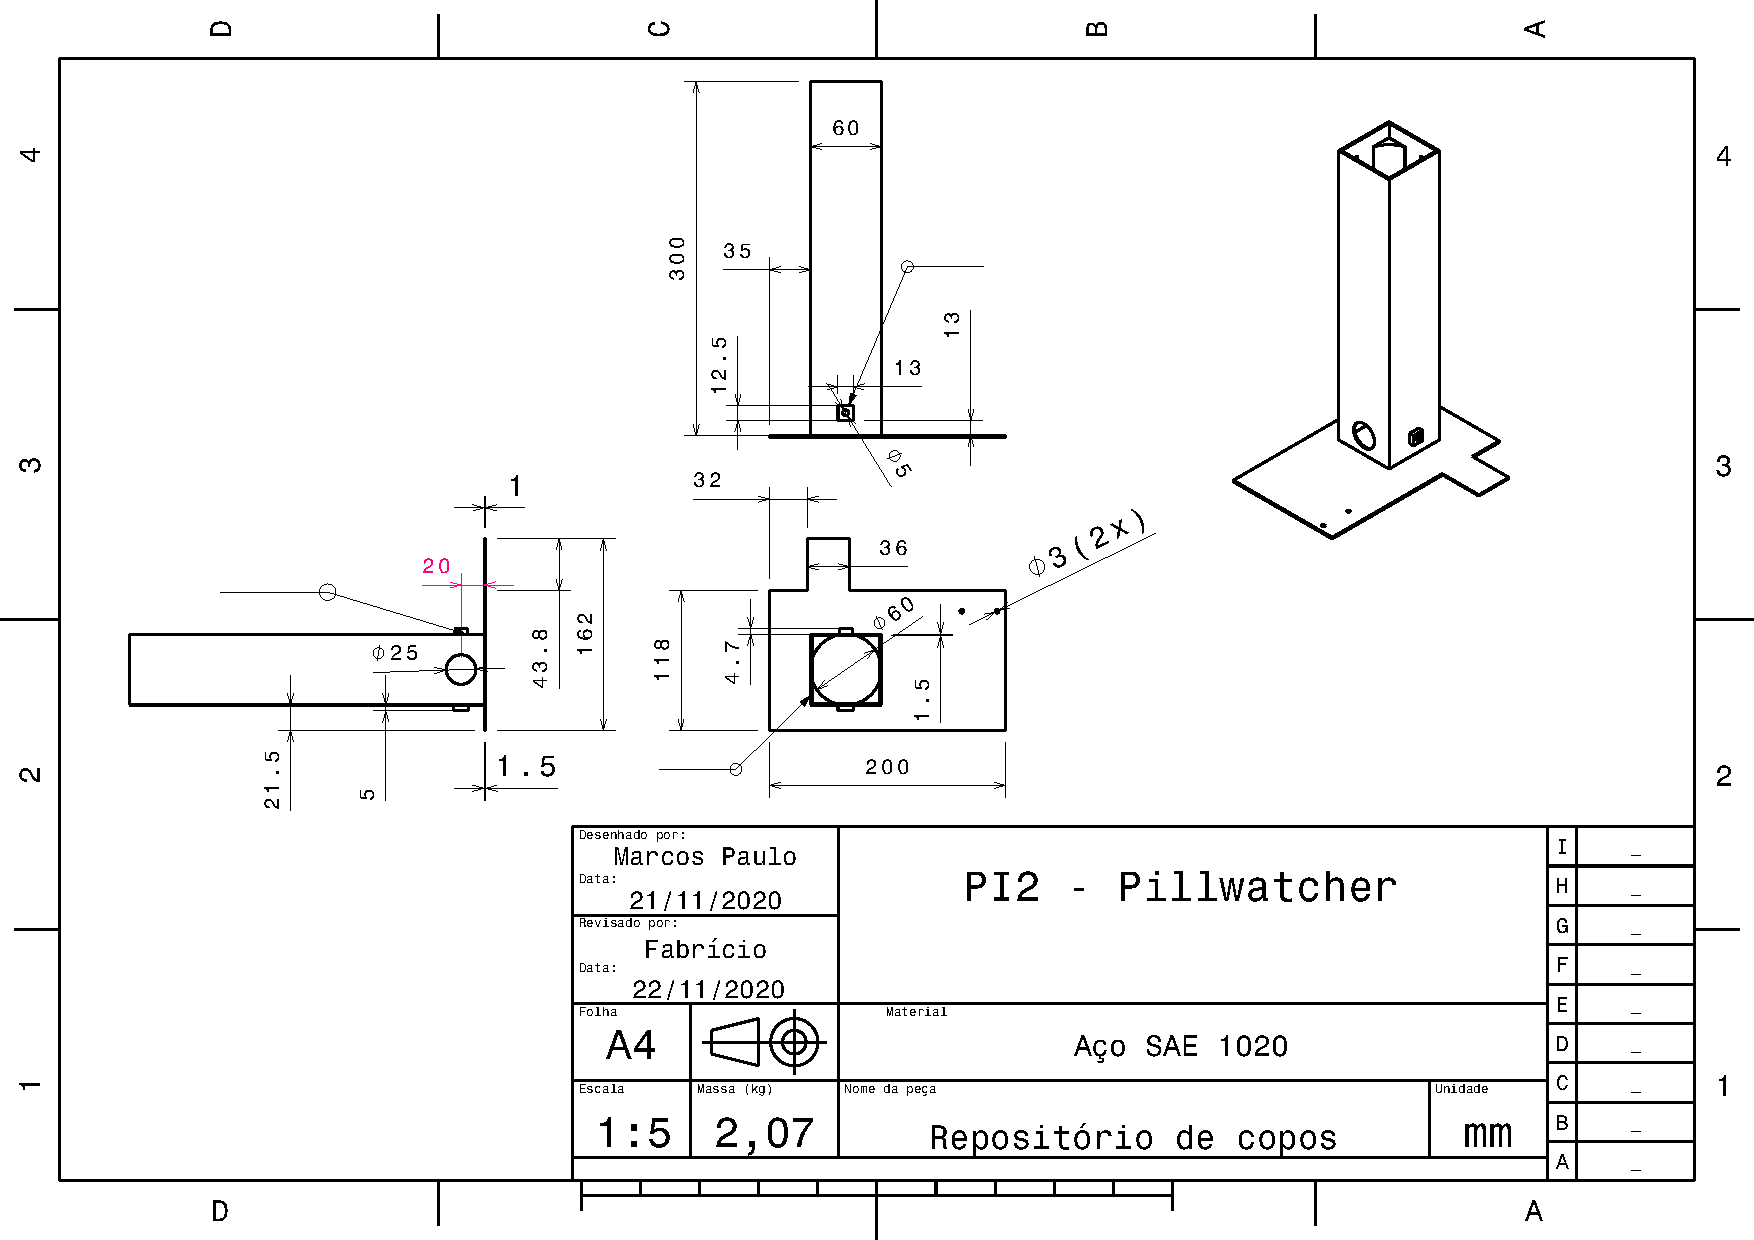
\includegraphics[width=0.9\textwidth]{figuras/estrutura/Desenhos/Reservatorio_V2.pdf}
    \caption{Desenho técnico do repositório de copos (\ref{retorno_reservatorio})}
    \label{fig:repositorio}
\end{figure}

\begin{figure}[H]
    \centering
    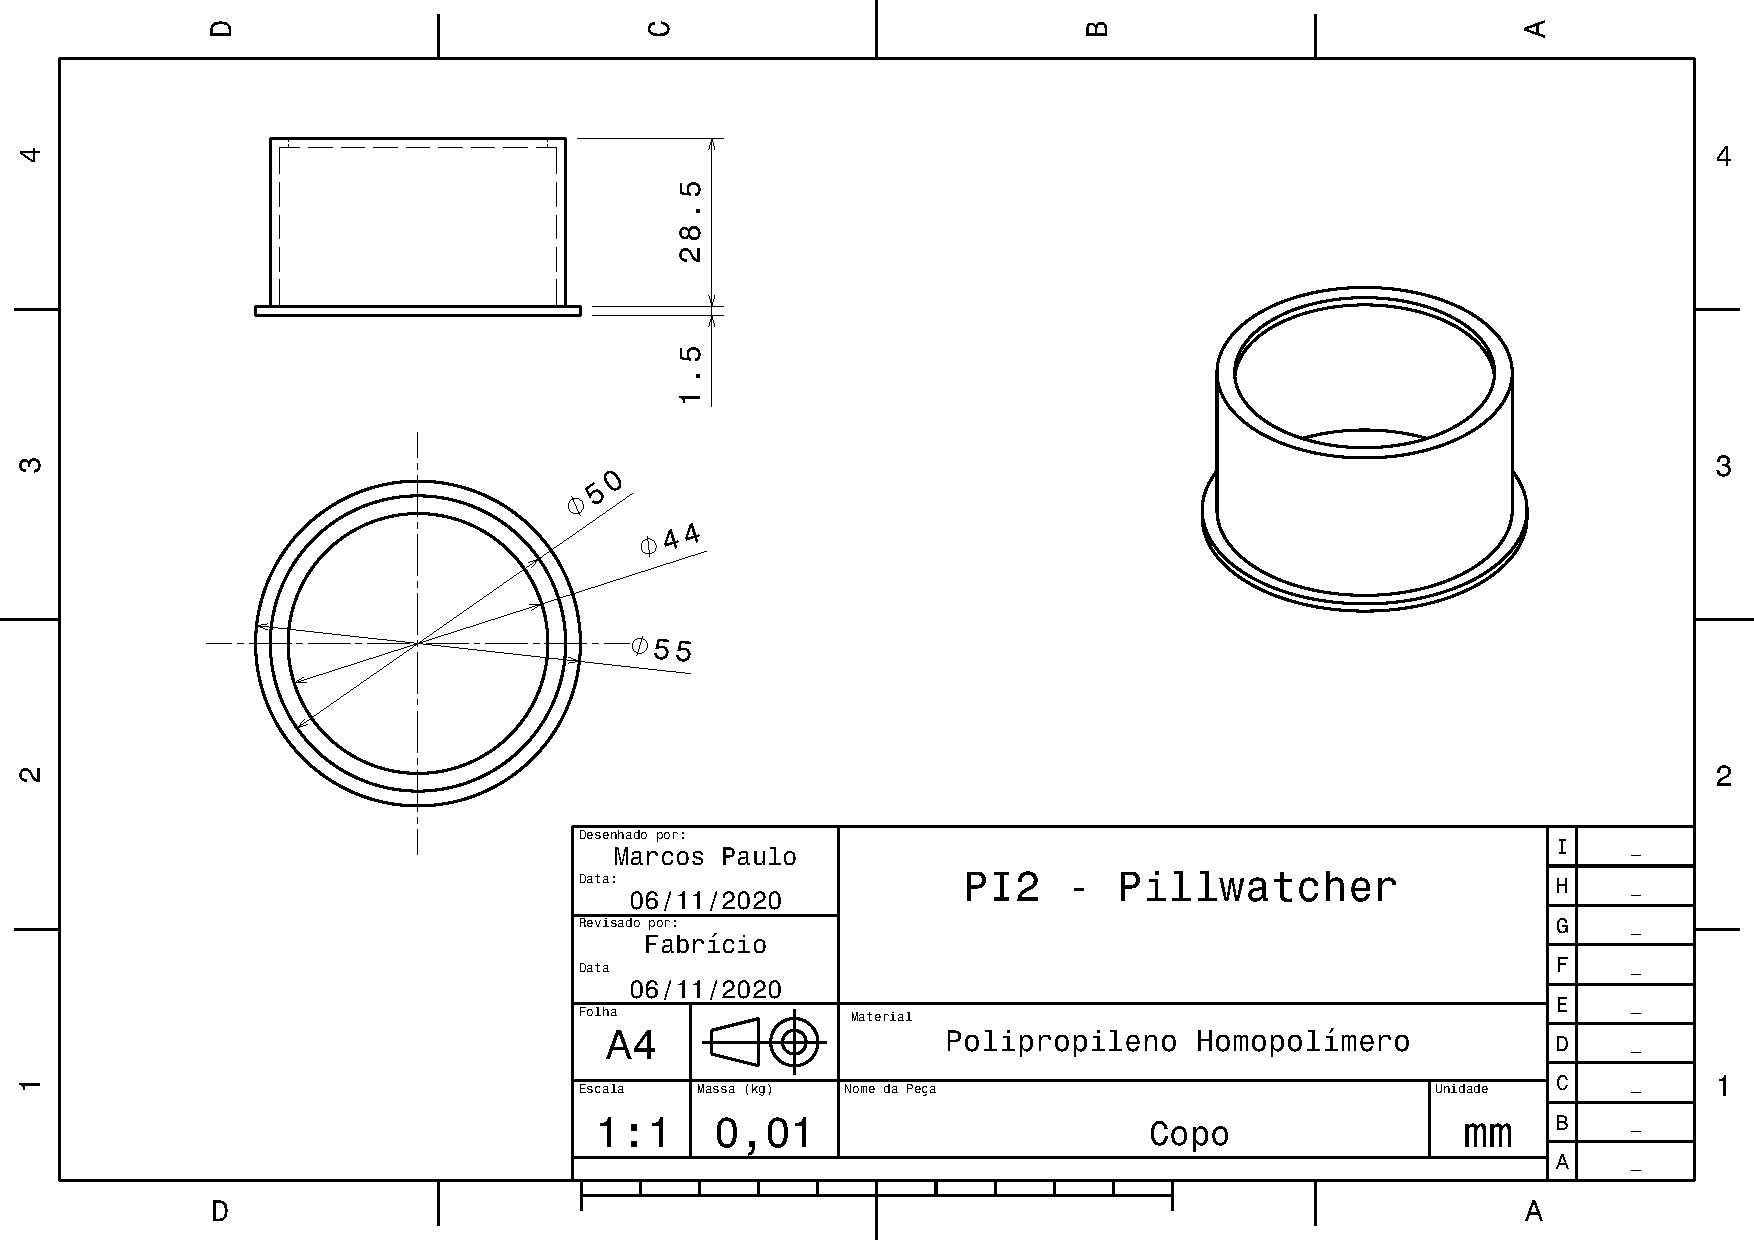
\includegraphics[width=0.9\textwidth]{figuras/estrutura/Desenhos/Copo.pdf}
    \caption{Desenho técnico do copo de medicamentos (\ref{retorno_copo})}
    \label{fig:copo}
\end{figure}

\begin{figure}[H]
    \centering
    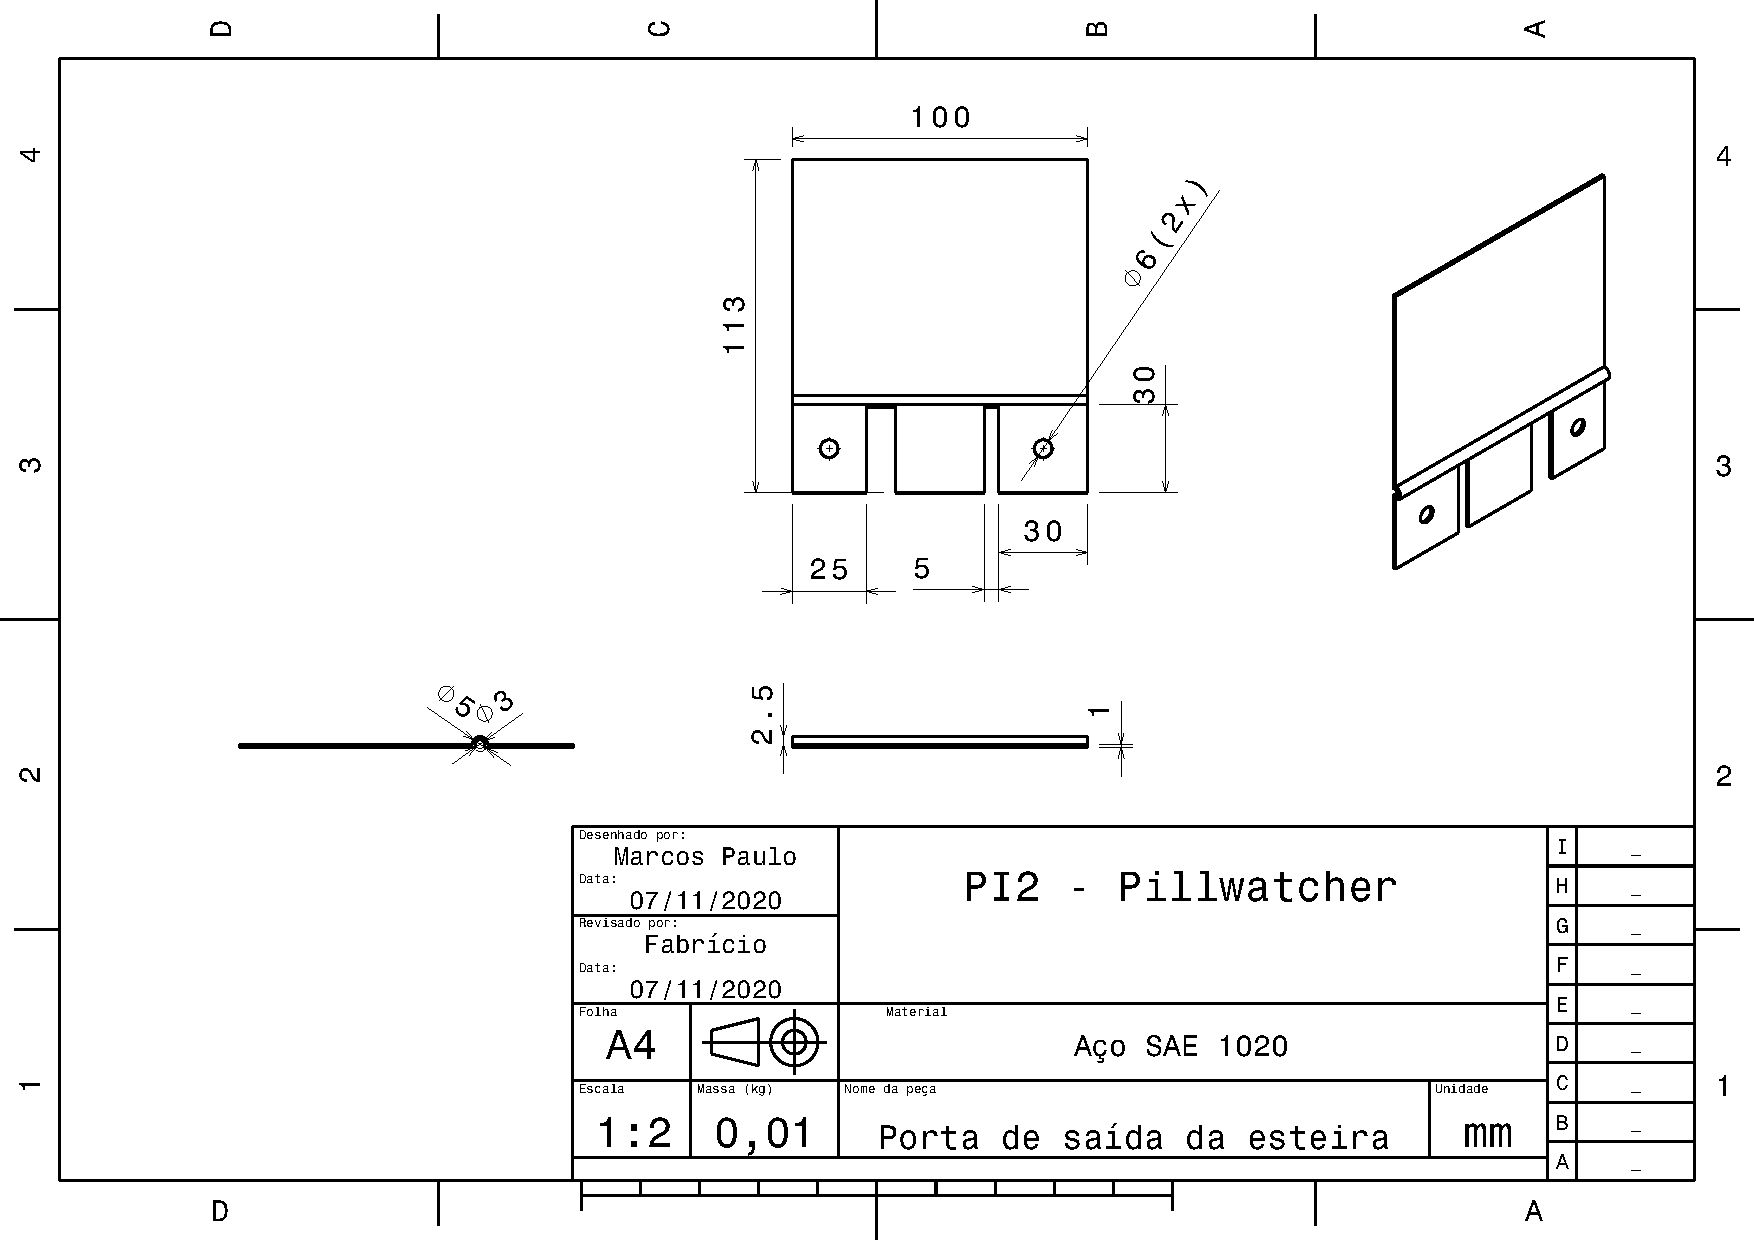
\includegraphics[width=0.8\textwidth]{figuras/estrutura/Desenhos/Porta_Saida.pdf}
    \caption{Desenho técnico da porta de saída, que se apresenta tanto na saída verdadeira quanto na saída de retorno (\ref{retorno_porta})}
    \label{fig:porta_saida}
\end{figure}

\begin{figure}[H]
    \centering
    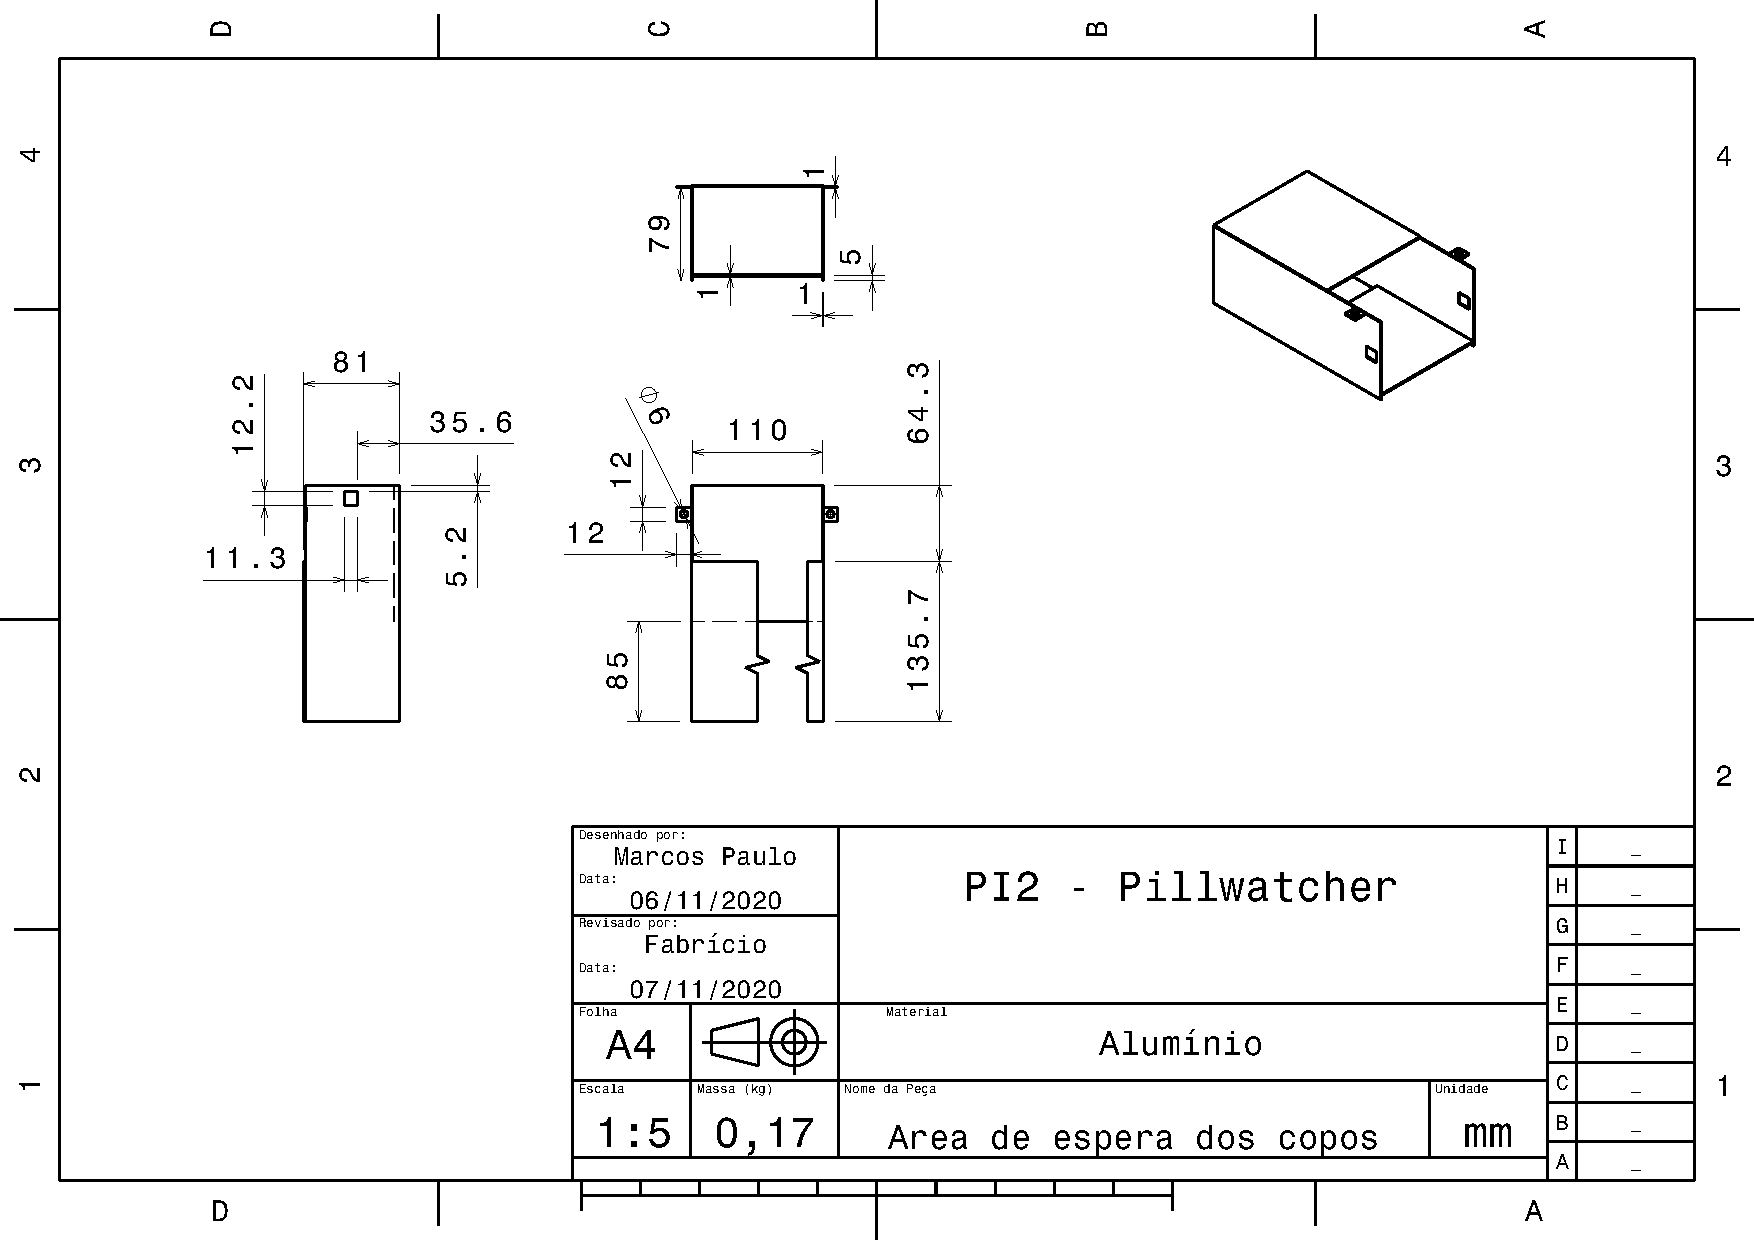
\includegraphics[width=0.8\textwidth]{figuras/estrutura/Desenhos/Area de espera dos copos.pdf}
    \caption{Desenho técnico da área de espera dos copos, na face frontal da estrutura (\ref{retorno_porta})}
    \label{fig:area_espera}
\end{figure}

\begin{figure}[H]
    \centering
    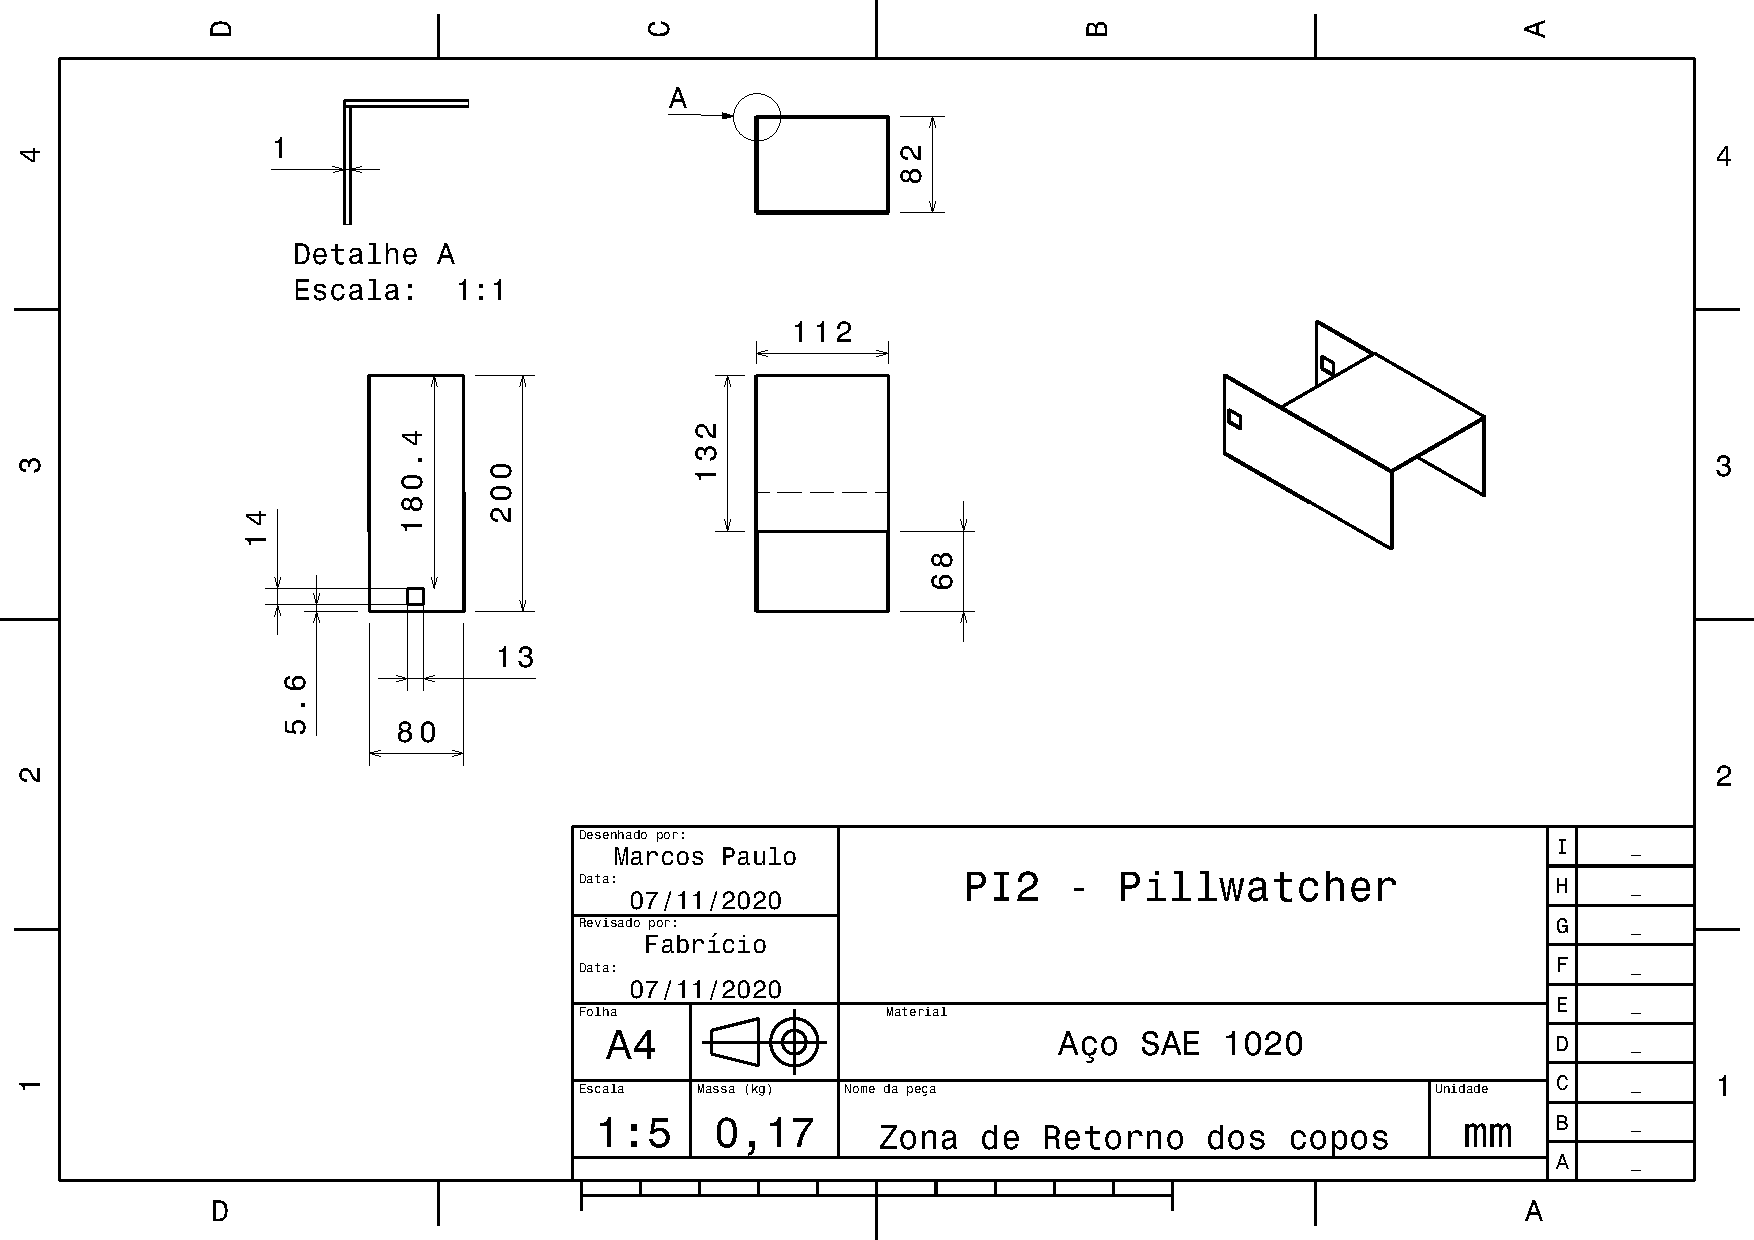
\includegraphics[width=0.8\textwidth]{figuras/estrutura/Desenhos/Zona_retorno.pdf}
    \caption{Desenho técnico da zona de retorno, na face anterior da estrutura (\ref{retorno_porta})}
    \label{fig:zona_retorno}
\end{figure}

\begin{figure}[H]
    \centering
    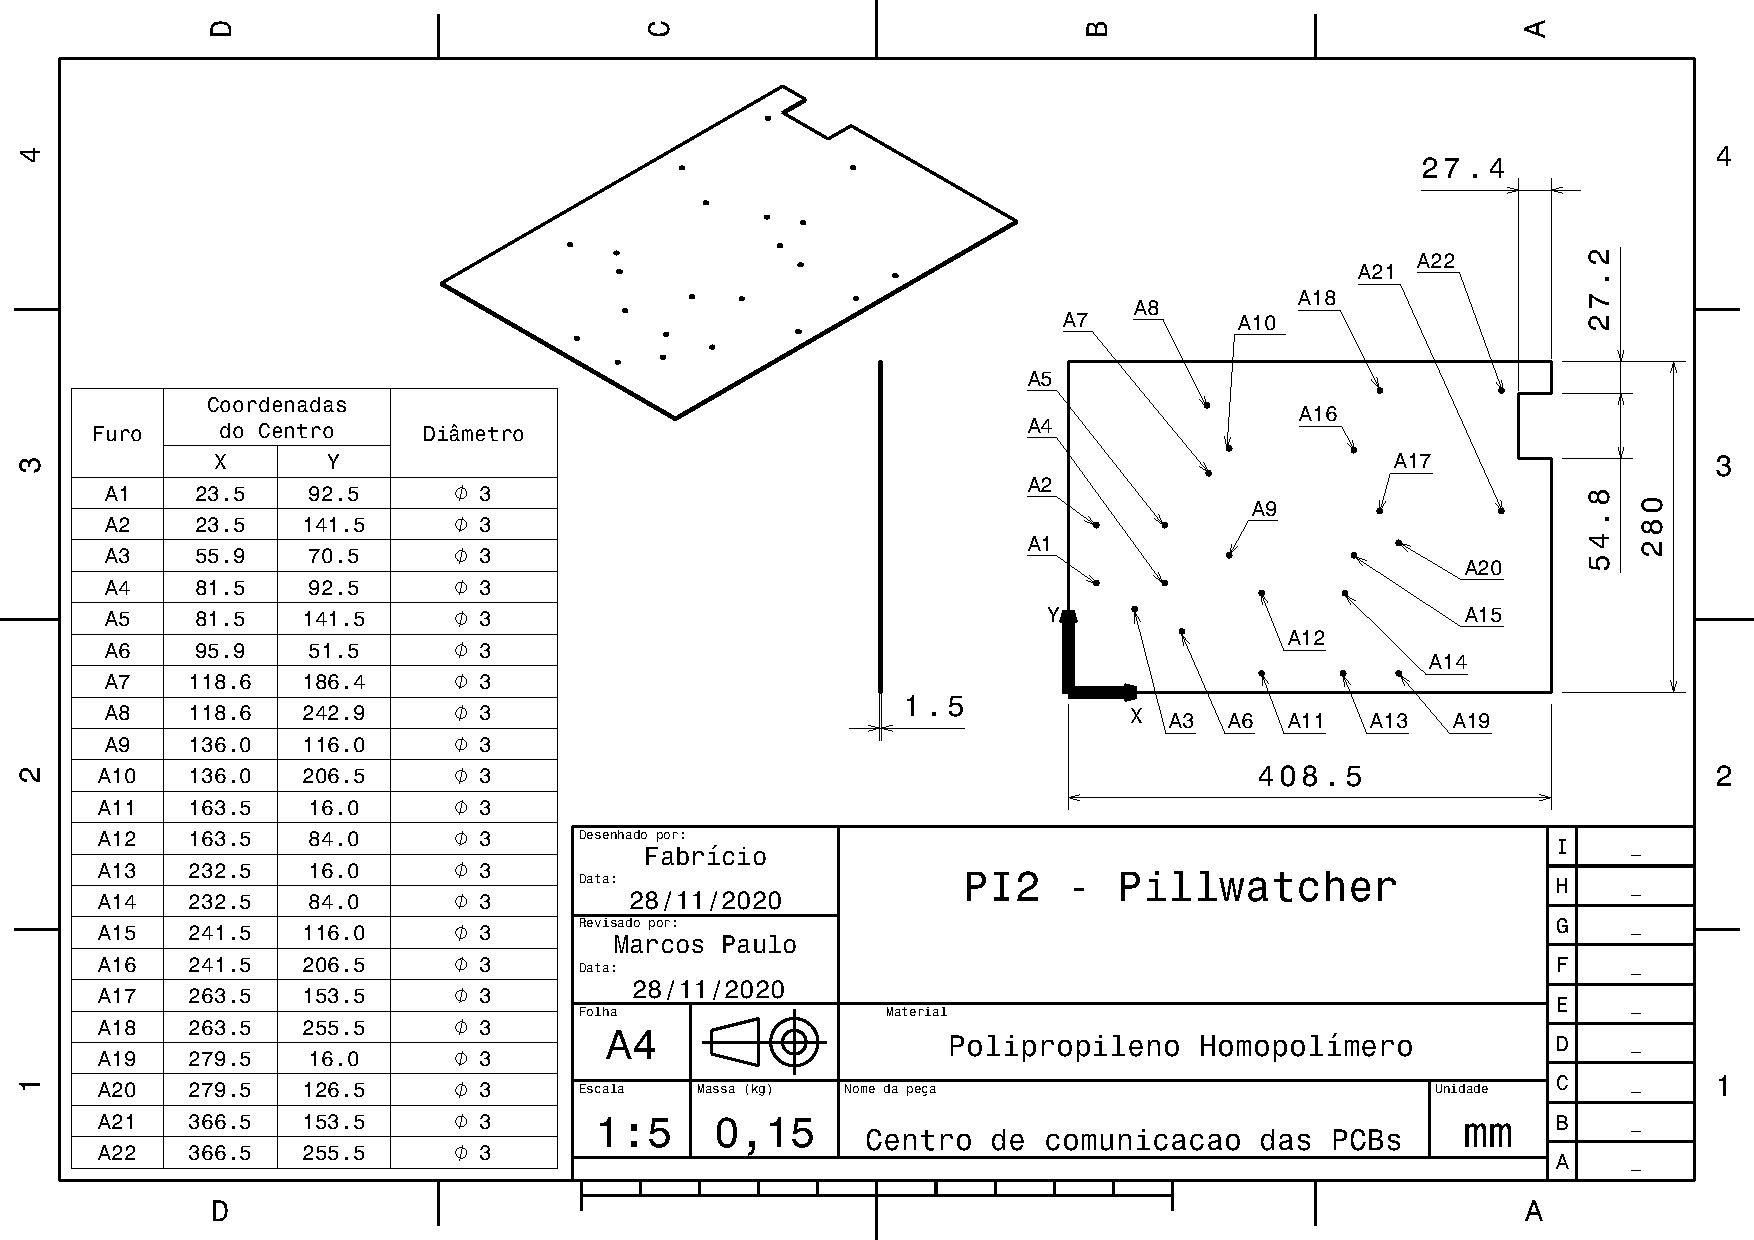
\includegraphics[width=0.8\textwidth]{figuras/estrutura/Desenhos/Centro_Comunicacao_V3.pdf}
    \caption{Desenho técnico do centro de comunicação das PCBs (\ref{retorno_Centro_PCBs})}
    \label{fig:Centro_PCBs}
\end{figure}

\begin{figure}[H]
    \centering
    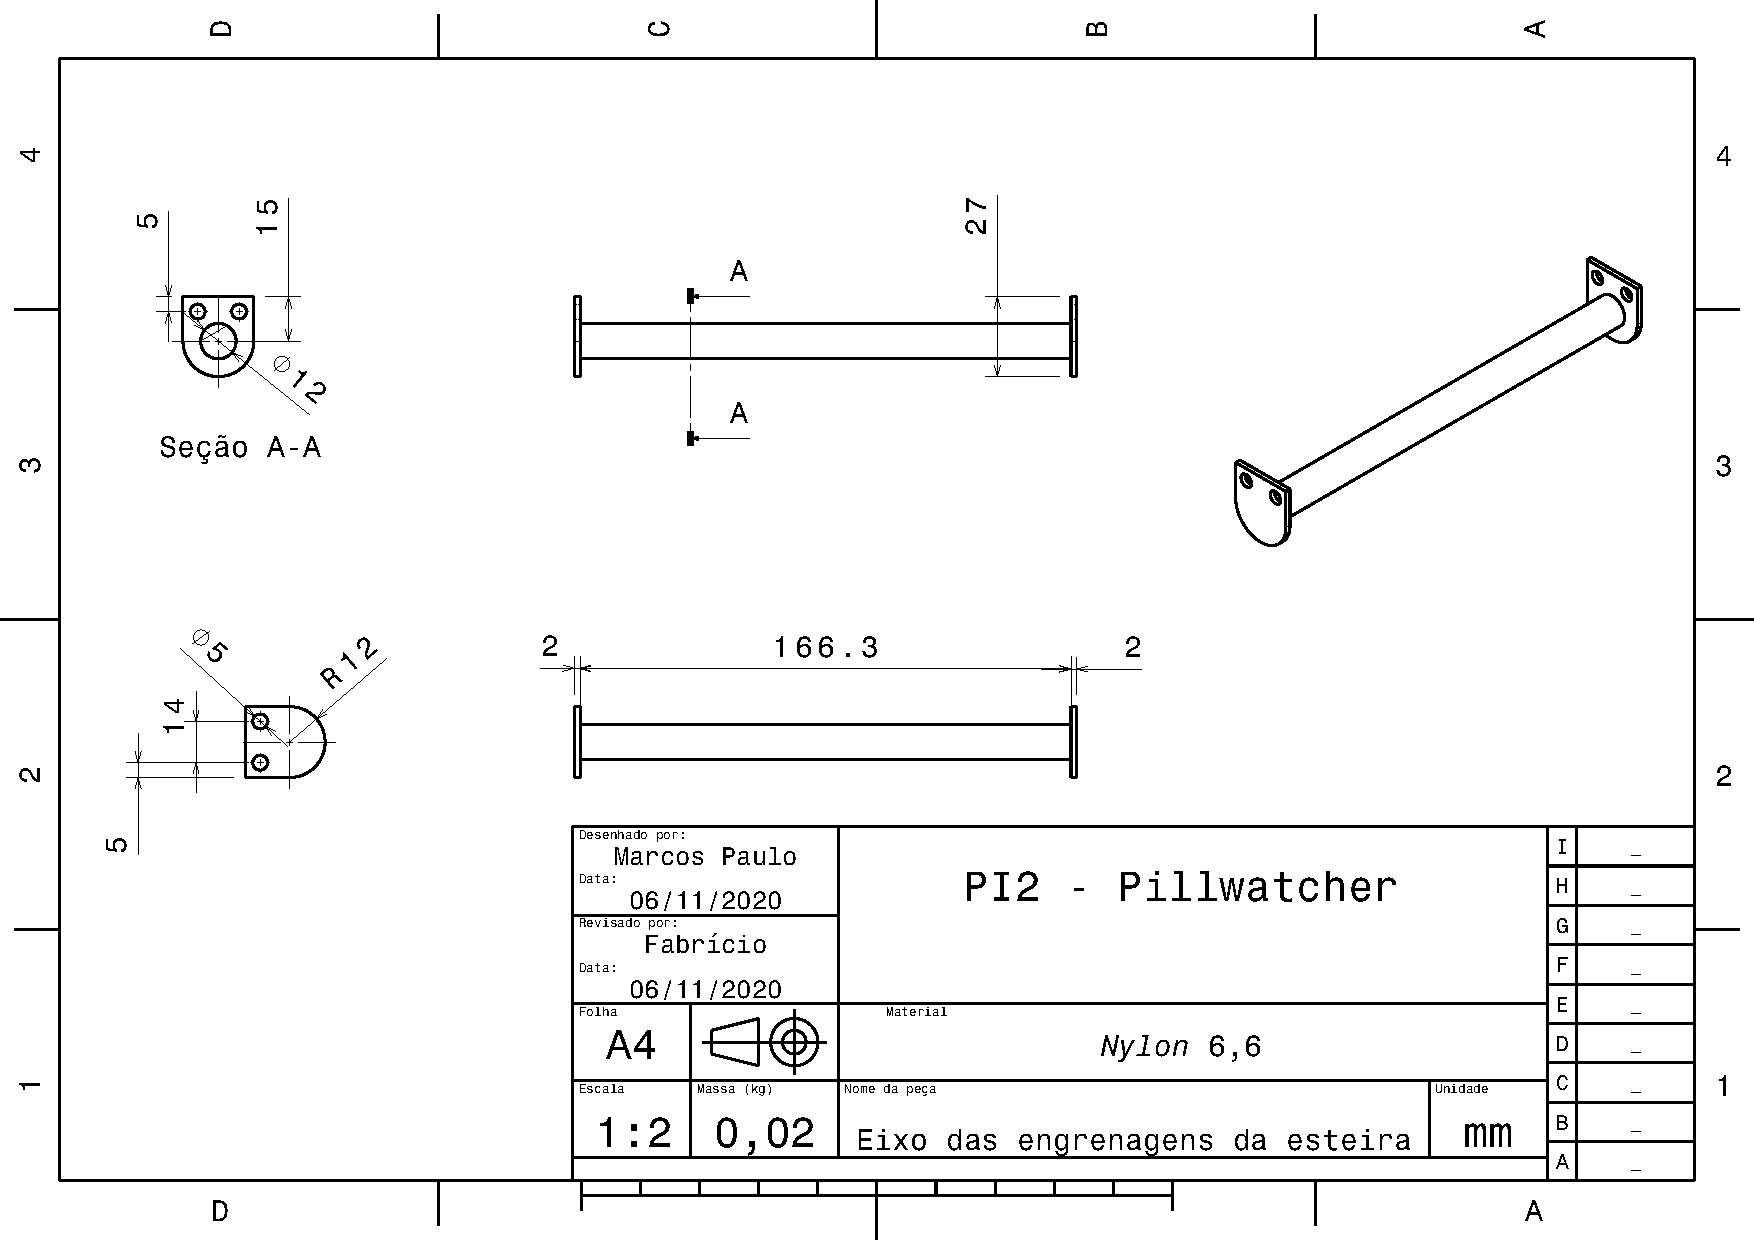
\includegraphics[width=0.8\textwidth]{figuras/estrutura/Desenhos/Eixo_Esteira.pdf}
    \caption{Desenho técnico dos eixos de suporte das engrenagens da esteira (\ref{retorno_Eixos_Esteira})}
    \label{fig:Eixos_Esteira}
\end{figure}

\begin{figure}[H]
    \centering
    \includegraphics[width=0.8\textwidth]{figuras/estrutura/Desenhos/Centro_Alimentacao_V2.pdf}
    \caption{Desenho técnico do suporte dos componentes energéticos, chamado Centro de Alimentação (\ref{retorno_suporte_energia})}
    \label{fig:suporte_energia}
\end{figure}

\begin{figure}[H]
    \centering
    \includegraphics[width=0.8\textwidth]{figuras/estrutura/Desenhos/Suporte_interruptor.pdf}
    \caption{Desenho técnico do suporte das chaves interruptoras (\ref{retorno_suporte_interruptor})}
    \label{fig:suporte_interruptor}
\end{figure}

\begin{figure}[H]
    \centering
    \includegraphics[width=0.8\textwidth]{figuras/estrutura/Desenhos/Rolamento_fuso.pdf}
    \caption{Desenho técnico do rolamento do mancal do fuso (\ref{Retorno_Mancal_de_suporte})}
    \label{fig:rolamento_fuso}
\end{figure}

\begin{figure}[H]
    \centering
    \includegraphics[width=0.8\textwidth]{figuras/estrutura/Desenhos/Solda_Base_Tubos.pdf}
    \caption{Indicações de solda da base de contêineres na estrutura tubular(\ref{section:fabricacao})}
    \label{fig:Solda_Base_Estrutura}
\end{figure}

\begin{figure}[H]
    \centering
    \includegraphics[width=0.8\textwidth]{figuras/estrutura/Desenhos/Solda_Suporte_MotorPasso.pdf}
    \caption{Indicações de solda do suporte dos motores de passo na estrutura tubular(\ref{section:fabricacao})}
    \label{fig:Solda_Supp_MotorPasso}
\end{figure}

\begin{figure}[H]
    \centering
    \includegraphics[width=0.8\textwidth]{figuras/estrutura/Desenhos/Solda_Suporte_MotorDC.pdf}
    \caption{Indicações de solda do suporte do motor DC na estrutura tubular(\ref{section:fabricacao})}
    \label{fig:Solda_Supp_MotorDC}
\end{figure}

\begin{figure}[H]
    \centering
    \includegraphics[width=0.8\textwidth]{figuras/estrutura/Desenhos/Solda_fotossensores.pdf}
    \caption{Indicações de solda dos suportes dos sensores fotoelétricos em toda a estrutura(\ref{pos_compontes})}
    \label{fig:Solda_Supp_fotossensores}
\end{figure}

\begin{figure}[H]
    \centering
    \includegraphics[width=0.9\textwidth]{figuras/estrutura/Design/Vista completa com circuitaria.png}
    \caption{Estrutural Global em formato CAD}
    \label{fig:global}
\end{figure}

\begin{figure}[H]
    \centering
    \includegraphics[width=0.7\textwidth]{figuras/estrutura/Design/ChapasExterior.jpeg}
    \caption{Carcaça da estrutura formato CAD}
    \label{fig:Carcaca}
\end{figure}

\begin{figure}[H]
    \centering
    \includegraphics[width=0.7\textwidth]{figuras/estrutura/Porta de saída.png}
    \caption{Porta de saída}
    \label{fig:portas}
\end{figure}

\begin{figure}[H]
    \centering
    \includegraphics[width=0.7\textwidth]{figuras/estrutura/Copo.png}
    \caption{Ilustração do Copo}
    \label{fig:copos}
\end{figure}

\begin{figure}[H]
    \centering
    \includegraphics[width=1\textwidth]{figuras/estrutura/Motor de Passo no Fuso.png}
    \caption{Motor de passo com fuso}
    \label{fig:motordepassonofuso}
\end{figure}

\begin{figure}[H]
    \centering
    \includegraphics[width=0.9\textwidth]{figuras/estrutura/Recipiente dos Copos + Esteira.png}
    \caption{Reservatório de copos com esteira}
    \label{fig:reservatorioCopos}
\end{figure}

\begin{figure}[H]
    \centering
    \includegraphics[width=0.8\textwidth]{figuras/estrutura/Detalhe Fuso com Engrenagem.png}
    \caption{Detalhes do fuso com engrenagens}
    \label{fig:fusoEngrenagens}
\end{figure}   

\begin{figure}[H]
    \centering
    \includegraphics[width=0.6\textwidth]{figuras/estrutura/Conteiner.png}
    \caption{Contêiner dos medicamentos}
    \label{fig:conteiner}
\end{figure}

\begin{figure}[H]
    \centering
    \includegraphics[width=0.6\textwidth]{figuras/estrutura/Descrição Contêiner.png}
    \caption{Descrição detalhada do contêiner}
    \label{fig:DescricaoConteiner}
\end{figure}


%\begin{figure}[H]
%    \centering
%    \includegraphics[width=0.8\textwidth]{figuras/estrutura/Perfil Quadrado.png}
%    \caption{Cotagem do Tubo}
%    \label{fig:Cotastubo}
%\end{figure}    

\chapter{\textit{Mockup} das Telas do Visor}\label{app_telas_display}

A Central de Controle exibirá no visor para usuário os avisos e status dos sistemas que compõem o projeto. Assim, para a inicialização do dispositivo, deve-se realizar o cadastro no aplicativo do número de série disponível no visor, conforme a Fig. \ref{fig:app_tela_1}. Em seguida, o usuário irá selecionar uma rede de internet para fazer o login, segundo a Fig. \ref{fig:app_tela_2}. Posteriormente, deve-se digitar a senha, por meio da utilização da matriz de botões no teclado virtual disponível no visor, na Fig. \ref{fig:app_tela_3}. 

\begin{figure}[H]
    \centering
    \subfloat[][Tela Inicial com Número de série]{
    \includegraphics[width=4.3cm]{figuras/eletronica/telas_dispositivo/1.png}
    \label{fig:app_tela_1}}
    \subfloat[][Tela de seleção Inicial de Rede]{
    \includegraphics[width=4.3cm]{figuras/eletronica/telas_dispositivo/2.png}
    \label{fig:app_tela_2}}
    \subfloat[][Tela de conexão]{
    \includegraphics[width=4.3cm]{figuras/eletronica/telas_dispositivo/3.png}
    \label{fig:app_tela_3}}
    \caption{Telas de Iniciação}\label{fig:telas_1_2_3}
\end{figure}

A Fig. \ref{fig:app_tela_4} apresenta a tela inicial no modo de espera, com horário, data, item de conexão com a internet, item da conexão do dispositivo com a rede elétrica e quando o dispositivo está utilizando a bateria, em casos de falta de energia. Além do mais, a partir da tela inicial, é possível acessar as configurações e a agenda de medicamentos. Assim, conforme a Fig. \ref{fig:app_tela_24}, existe a representação da agenda da próxima hora de medicações dos pacientes, por ordem de horário.

\begin{figure}[!htb]
    \centering
    \subfloat[][Tela Inicial]{
    \includegraphics[width=4.3cm]{figuras/eletronica/telas_dispositivo/4.png}
    \label{fig:app_tela_4}}
    \subfloat[][Tela da agenda com medicações]{
    \includegraphics[width=4.3cm]{figuras/eletronica/telas_dispositivo/24.png}
    \label{fig:app_tela_24}}
    \caption{Tela Inicial e Tela da Agenda}\label{fig:telas_4_24}
\end{figure}

Ao clicar, utilizando a matriz de botões no ícone das configurações, o usuário é encaminhado para um menu \ref{fig:app_tela_9}. Nele, é possível alterar a rede de conexão com a internet \ref{fig:app_tela_10}, alterar data e hora \ref{fig:app_tela_11}, alterar o brilho da tela \ref{fig:app_tela_12} e acessar a tela com informações técnicas do dispositivo \ref{fig:app_tela_13}.

\begin{figure}[H]
    \centering
    \subfloat[][Tela de configurações]{
    \includegraphics[width=4.3cm]{figuras/eletronica/telas_dispositivo/9.png}
    \label{fig:app_tela_9}}
    \subfloat[][Tela de alteração de rede]{
    \includegraphics[width=4.3cm]{figuras/eletronica/telas_dispositivo/10.png}
    \label{fig:app_tela_10}}
    \subfloat[][Tela de alteração da data e hora]{
    \includegraphics[width=4.3cm]{figuras/eletronica/telas_dispositivo/11.png}
    \label{fig:app_tela_11}}
    \caption{Telas de Configuração - Parte 1}\label{fig:telas_9_10_11}
\end{figure}

\begin{figure}[H]
    \centering
    \subfloat[][Tela de alteração do brilho da tela]{
    \includegraphics[width=4.3cm]{figuras/eletronica/telas_dispositivo/12.png}
    \label{fig:app_tela_12}}
    \subfloat[][Tela com informações do dispositivo]{
    \includegraphics[width=4.3cm]{figuras/eletronica/telas_dispositivo/13.png}
    \label{fig:app_tela_13}}
    \caption{Telas de Configuração - Parte 2}\label{fig:telas_12_13}
\end{figure}

A Fig. \ref{fig:app_tela_5} representa o processo de dispensação da dose de medicamentos individuais, uma vez que existem pacientes que necessitam de mais de uma medicação no mesmo horário. Após o final do processo de separação da dose de medicamentos, tem-se um aviso no visor que o medicamento já pode ser retirado do dispositivo, com tela representada na Fig. \ref{fig:app_tela_6}. Após o aviso da Fig. \ref{fig:app_tela_6}, é apresentado no visor as doses de medicamentos que já estão prontas para retirada, com a cor do copo dos medicamentos, o nome do paciente e o horário da administração, conforme a Fig. \ref{fig:app_tela_7}.

\begin{figure}[H]
    \centering
    \subfloat[][Tela do processo de dispensação]{
    \includegraphics[width=4.3cm]{figuras/eletronica/telas_dispositivo/5.png}
    \label{fig:app_tela_5}}
    \subfloat[][Tela de aviso do final do processo de dispensação]{
    \includegraphics[width=4.3cm]{figuras/eletronica/telas_dispositivo/6.png}
    \label{fig:app_tela_6}}
    \subfloat[][Tela com a lista de pacientes e medicamentos dispensados]{
    \includegraphics[width=4.3cm]{figuras/eletronica/telas_dispositivo/7.png}
    \label{fig:app_tela_7}}
    \caption{Telas de Dispensação do Medicamento}\label{fig:telas_5_6_7}
\end{figure}

Nas figuras \ref{fig:telas_14_15_16}, \ref{fig:telas_17_19_20} e \ref{fig:telas_18_8} estão representadas as telas de aviso. Sendo assim, as telas \ref{fig:app_tela_14} e \ref{fig:app_tela_15} avisam o enfermeiro quando as portas estão abertas e se os contêineres estão mal encaixados, após o processo de reabastecimento. Já a tela \ref{fig:app_tela_16} avisa a existência de copos com medicamentos na comporta traseira, sendo estas as doses medicamentosas reprovadas por apresentar uma quantidade de medicamentos incorreta ou tipo de medicação errada, após processamento de imagem. 


\begin{figure}[H]
    \centering
    \subfloat[][Aviso Porta Aberta]{
    \includegraphics[width=4.3cm]{figuras/eletronica/telas_dispositivo/14.png}
    \label{fig:app_tela_14}}
    \subfloat[][Aviso contêiner mal encaixado]{
    \includegraphics[width=4.3cm]{figuras/eletronica/telas_dispositivo/15.png}
    \label{fig:app_tela_15}}
    \subfloat[][Aviso de medicamentos no compartimento traseiro]{
    \includegraphics[width=4.3cm]{figuras/eletronica/telas_dispositivo/16.png}
    \label{fig:app_tela_16}}
    \caption{Telas de Aviso - Parte 1 }\label{fig:telas_14_15_16}
\end{figure}

A tela \ref{fig:app_tela_17} avisa quando não há conexão com a internet. Nesse caso, o dispositivo terá uma redução de atividades de adição de medicamento, enfermeiro ou paciente. A tela \ref{fig:app_tela_18} avisa quando não tem a conexão com a rede elétrica, situação na qual o dispositivo troca automaticamente a fonte de alimentação da principal para bateria reserva. Após algumas horas de uso da bateria, aparece a tela com aviso  da bateria estar acabando, conforme representado na Fig. \ref{fig:app_tela_20}.

\begin{figure}[H]
    \centering
    \subfloat[][Aviso sem conexão com a internet]{
    \includegraphics[width=4.3cm]{figuras/eletronica/telas_dispositivo/17.png}
    \label{fig:app_tela_17}}
    \subfloat[][Aviso sem energia]{
    \includegraphics[width=4.3cm]{figuras/eletronica/telas_dispositivo/19.png}
    \label{fig:app_tela_19}}
    \subfloat[][Aviso bateria acabando]{
    \includegraphics[width=4.3cm]{figuras/eletronica/telas_dispositivo/20.png}
    \label{fig:app_tela_20}}
    \caption{Telas de Aviso - Parte 2}\label{fig:telas_17_19_20}
\end{figure}

A tela \ref{fig:app_tela_18} avisa para o enfermeiro no momento da seleção de medicamento quando existe um medicamento. Ou seja, quando não ocorre a detecção do medicamento pelo sensor de barreira localizado no funil, pode-se concluir que o medicamento ficou preso no dispositivo. Já a tela \ref{fig:app_tela_8} avisa para o enfermeiro que existe uma medicação atrasada, disponível para ser retirada no dispositivo.

\begin{figure}[H]
    \centering
    \subfloat[][Aviso medicamento preso no dispositivo]{
    \includegraphics[width=4.3cm]{figuras/eletronica/telas_dispositivo/18.png}
    \label{fig:app_tela_18}}
    \subfloat[][Aviso no atrasado da retirada de medicação]{
    \includegraphics[width=4.3cm]{figuras/eletronica/telas_dispositivo/8.png}
    \label{fig:app_tela_8}}
    \caption{Telas de Aviso - Parte 3}\label{fig:telas_18_8}
\end{figure}


\begin{figure}[H]
    \centering
    \subfloat[][Tela de cadastro de biometria]{
    \includegraphics[width=4.3cm]{figuras/eletronica/telas_dispositivo/22.png}
    \label{fig:app_tela_22}}
    \subfloat[][Tela de biometria aceita]{
    \includegraphics[width=4.3cm]{figuras/eletronica/telas_dispositivo/23.png}
    \label{fig:app_tela_23}}
    \caption{Telas de Biometria}\label{fig:telas_22_23}
\end{figure}
Todos os cadastros serão realizados no aplicativo. Entretanto, para o enfermeiro terminar o seu cadastro, ele necessita colocar sua digital para registar a biometria. Sendo assim, é necessária uma tela para informar o horário correto de posicionar a digital, como demostrado na Fig. \ref{fig:app_tela_22}. Em seguida, quando a leitura da digital é concluída tanto no processo do cadastro quanto para retirar ou adicionar medicamentos do dispositivo, será mostrado a tela no visor representado na Fig. \ref{fig:app_tela_23}.


\begin{figure}[H]
    \centering
    \subfloat[][Tela do modo de reabastecimento]{
    \includegraphics[width=4.3cm]{figuras/eletronica/telas_dispositivo/21.png}
    \label{fig:app_tela_21}}
    \subfloat[][Tela de desligamento]{
    \includegraphics[width=4.3cm]{figuras/eletronica/telas_dispositivo/25.png}
    \label{fig:app_tela_25}}
    \caption{Telas de Reabastecimento e desligamento }\label{fig:telas_21_25}
\end{figure}

A tela \ref{fig:app_tela_21} informa ao enfermeiro que o dispositivo está no modo de reabastecimento, logo, todas as funcionalidades da máquina estão suspensas. A tela \ref{fig:app_tela_25} é utilizada como uma verificação para se realizar o desligamento do dispositivo.

\chapter{Esquemáticos Eletrônicos}\label{esquematicos_eletronica}

Os esquemáticos de conexão entre os componentes da solução eletrônica foram divididos em 5 esquemáticos. A divisão foi realizada levando em consideração que cada esquemático será a base para criação da respectiva placa de circuito impresso (PCI).

No esquemático 1, na Fig. \ref{fig:esquematico_1}, temos representado as conexões da \textit{Raspberry Pi} 4 com o sensor de biometria DY50, sensor de temperatura e umidade HTU21D, sensor RFID PN532, a câmera OV5647, o LCD 240x320 e os quatro microcontroladores PIC16F677. Também está representada a conexão da fonte de alimentação 5 V (+5 V e GND), fornecida pela solução energética. 

Para os microcontroladores PIC16 1, PIC16 2, PIC16 3 e PIC16 4 temos os pinos de alimentação e os 2 pinos SDA e SCL da comunicação por protocolo I$^2$C. De forma semelhante, temos os mesmos pinos para o módulo controlador RFID PN53. Para o sensor de temperatura e umidade, temos alimentação de +3,3 V vinda da \textit{Raspberry Pi} 4  (Pino 1 - GPIO 1) e os pinos da comunicação por protocolo I$^2$C. O sensor de biometria DY50 é alimentado por 5 V e conectado aos pinos de comunicação do protocolo UART (TXD, RXD). O visor LCD 240x320 tem a conexão dos pinos de alimentação para 5 V e a conexão do protocolo SPI com a \textit{Raspberry Pi} 4. Por fim, temos uma representação esquemática da conexão do protocolo CSI pelo soquete ZIF 15 pinos da \textit{Raspberry Pi} 4 e sua conexão com a câmera OV5647.

\begin{landscape}
\begin{figure}[H]
    \centering
    \vspace{-2cm}
    \includegraphics[width=1.25\textwidth, height=2\textheight,keepaspectratio]{figuras/eletronica/esquematicos/esquematico_1_rpi4.pdf}
    \caption{Diagrama esquemático da conexão das Raspberry Pi 4 com sensores e microcontroladores}
    \label{fig:esquematico_1}
\end{figure}
\end{landscape}


A PIC16 1 é a conexão com o microcontrolador  responsável por receber os dados dos sensores de barreira, com representação esquemática na Fig. \ref{fig:esquematico_2}. Neste esquemático, temos representado a conexão entre o microcontrolador e os 30 sensores de barreira, onde cada sensor precisa ser conectado com um conector de 3 pinos (5 V, GND e OUT). Dos 30 sensores, 24 estão conectados nos 3 multiplexadores CD4051 e os 6 restantes estão diretamente no microcontrolador PIC16F677. Cada multiplexador precisa ser conectado com o microcontrolador com 4 pinos, sendo 3 para a seletora dos canais (A, B, C) e 1 de ativa à multiplexação (\textit{ENABLE}). Como forma de seleção, é comum a todos os multiplexadores e cada um pode ser ativado  individualmente pelo pino de \textit{ENABLE}. Os 9 pinos de seleção para os 3 multiplexadores são conectados nos mesmos 3 pinos I/O do microcontrolador, sendo os 3 pinos de \textit{ENABLE\_Bx} e de saída (\textit{MUX\_OUT\_Bx}) para cada multiplexador conectado ao restante das portas do microcontrolador.

A PIC16 2 é o microcontrolador responsável por receber os dados das chaves e traduzir as tensões analógicas do teclado para uma forma digital, utilizando a porta em que é conectado no modo conversor analógico digital, representação esquemática na Fig. \ref{fig:esquematico_3}. A conexão entre as 30 chaves segue a mesma lógica descrita para o microcontrolador do esquemático 2. No caso do teclado, temos que ele precisa de 3 pinos, sendo 2 de alimentação (5V e GND) e 1 da saída de dados (OUT\_TECLADO). Esses dados são tensões elétricas resultantes dos divisores de tensão do teclado. Portanto, foi necessário conectar a porta 9 (AN9) do microcontrolador, que pode ser configurada como um conversor analógico digital de 10 bits.


\begin{landscape}
\begin{figure}[H]
    \centering
    \includegraphics[width=1.25\textwidth, height=2\textheight,keepaspectratio]{figuras/eletronica/esquematicos/esquematico_2_micro1.pdf}
    \caption{Diagrama esquemático da conexão do microcontrolador 1 com os sensores de barreira}
    \label{fig:esquematico_2}
\end{figure}
\end{landscape}

\begin{landscape}
\begin{figure}[H]
    \centering
    \includegraphics[width=1.25\textwidth, height=2\textheight,keepaspectratio]{figuras/eletronica/esquematicos/esquematico_3_micro2.pdf}
    \caption{Diagrama esquemático da conexão do microcontrolador 2 com os interruptores e teclado}
    \label{fig:esquematico_3}
\end{figure}
\end{landscape}

A PIC16 3, com sua representação esquemática na Fig. \ref{fig:esquematico_4}, é o microcontrolador que traduz os sinais de controle advindos da \textit{Raspberry Pi} 4 para sinais lógicos dos \textit{drivers} IRF520N, responsáveis por controlar as solenoides e o atuador linear. A conexão com as 27 solenoides, utilizando os demultiplexadores, segue a mesma lógica do esquemático 3 e 4. Porém, ao invés de ser 1 saída de dados pra cada multiplexador, temos 1 entrada de dados (DEMUX\_IN\_SLx) e 8 saídas possíveis (SOLENOIDEx). Tanto o atuador linear quanto os 3 solenoides restantes (27 no total, sendo 24 conectados aos demux) são conectados diretamente a uma porta I/O do microcontrolador.

A PIC16 4, com sua representação esquemática na Fig. \ref{fig:esquematico_5}, é o microcontrolador que traduz os sinais de controle advindos da \textit{Raspberry Pi} 4 para sinais lógicos para os \textit{drivers} A4988 e Ponte H L298, que controlam os motores de passo e motor, respectivamente. Para o \textit{driver} Ponte H L298 do motor DC, temos a conexão com 3 pinos, sendo 2 (INx\_MOTOR\_DC) para controlar o motor A e 1 para a conexão da referência do circuito geral. Para os \textit{drivers} A4988, controle dos motores de passo, ocorre a conexão com o total de 9 pinos para cada um dos 5 utilizados, sendo 2 de alimentação (5V e GND), 6 pinos comuns entre os 5 \textit{drivers} (MS1, MS2, MS3, RESET, STEP e DIR) e o pino de \textit{EN\_MOTOR\_PASSO\_x}, exclusivo para cada motor de passo. Essa lógica vem dos 5 motores de passo realizarem o mesmo tipo de movimento, mas apenas um precisa estar ligado ao mesmo tempo. Ou seja, os 6 pinos são ligados aos mesmos 6 pinos no microcontrolador e são utilizados para realizar alguma ação de controle dos motores, enquanto o \textit{EN\_MOTOR\_PASSO\_x} ativa apenas o desejado naquele momento.

\begin{landscape}
\begin{figure}[H]
    \centering
    \includegraphics[width=1.25\textwidth, height=2\textheight,keepaspectratio]{figuras/eletronica/esquematicos/esquematico_4_micro3.pdf}
    \caption{Diagrama esquemático da conexão do microcontrolador 3 com os \textit{drivers} das solenoides e atuador linear}
    \label{fig:esquematico_4}
\end{figure}
\end{landscape}

\begin{landscape}
\begin{figure}[H]
    \centering
    \includegraphics[width=1.25\textwidth, height=2\textheight,keepaspectratio]{figuras/eletronica/esquematicos/esquematico_5_micro4.pdf}
    \caption{Diagrama esquemático da conexão do microcontrolador 4 com os \textit{drivers} dos motores de passo}
    \label{fig:esquematico_5}
\end{figure}
\end{landscape}

\chapter{Placas de Circuito Impresso (PCI)}\label{app:PCB}

\begin{figure}[H]
    \centering
    \subfloat[][Trilhas da PCI ]{
    \includegraphics[width=4.7cm]{figuras/eletronica/PCB/trilhas_sensor_barreira.png}
    \label{fig:trilhas_sensor_barreira}}
    \subfloat[][Vista superior da PCI]{
    \includegraphics[width=4.6cm]{figuras/eletronica/PCB/3D_sensor_barreira_1.png}
    \label{fig:3D_barreira}}
    \subfloat[][Vista inferior da PCI ]{
    \includegraphics[width=4.5cm]{figuras/eletronica/PCB/3D_sensor_barreira_2.png}
    \label{fig:3D_barreira_2}}
    \caption{PCI do sensor fotoelétrico de barreira}\label{fig:PCB_barreira}
\end{figure}
%\ref{fig:PCB_barreira}
%\ref{fig:PCB_central}
%\ref{fig:PCB_micro1}
%\ref{fig:PCB_micro2}
%\ref{fig:PCB_micro3}
%\ref{fig:PCB_micro4}
\begin{figure}[H]
    \centering
    \subfloat[][Trilhas da PCI]{
    \includegraphics[width=4.4cm]{figuras/eletronica/PCB/rasp.png}
    \label{fig:trilhas_2}}
    \subfloat[][Vista superior da PCI]{
    \includegraphics[width=4.3cm]{figuras/eletronica/PCB/raspfrente.png}
    \label{fig:3D_2}}
    \subfloat[][Vista inferior da PCI ]{
    \includegraphics[width=4.4cm]{figuras/eletronica/PCB/raspback.png}
    \label{fig:3D_3}}
    \caption{PCI do sistema central}\label{fig:PCB_central}
\end{figure}

\begin{figure}[H]
    \centering
    \subfloat[][Trilhas da PCI frente]{
    \includegraphics[width=4.3cm]{figuras/eletronica/PCB/micro1-1.png}
    \label{fig:trilhas_2_m11}}
    \subfloat[][Trilhas da PCI verso]{
    \includegraphics[width=4.3cm]{figuras/eletronica/PCB/micro1-2.png}
    \label{fig:trilhas_2_m112}}
    
    \subfloat[][Vista superior da PCI]{
    \includegraphics[width=4.3cm]{figuras/eletronica/PCB/micro1frente.png}
    \label{fig:3D_2_m12}}
    \subfloat[][Vista inferior da PCI ]{
    \includegraphics[width=4.3cm]{figuras/eletronica/PCB/micro1back.png}
    \label{fig:3D_3_m13}}
    \caption{PCI microcontrolador modelo 1}\label{fig:PCB_micro1}
\end{figure}

\begin{figure}[H]
    \centering
    \subfloat[][Trilhas da PCI frente]{
    \includegraphics[width=4.3cm]{figuras/eletronica/PCB/micro2-1.png}
    \label{fig:trilhas_2_m21}}
    \subfloat[][Trilhas da PCI verso]{
    \includegraphics[width=4.3cm]{figuras/eletronica/PCB/micro2-2.png}
    \label{fig:trilhas_2_m212}}
    
    \subfloat[][Vista superior da PCI]{
    \includegraphics[width=4.3cm]{figuras/eletronica/PCB/micro2frente.png}
    \label{fig:3D_2_m123}}
    \subfloat[][Vista inferior da PCI ]{
    \includegraphics[width=4.3cm]{figuras/eletronica/PCB/micro2back.png}
    \label{fig:3D_3_m23}}
    \caption{PCI microcontrolador modelo 2}\label{fig:PCB_micro2}
\end{figure}

\begin{figure}[H]
    \centering
    \subfloat[][Trilhas da PCI frente]{
    \includegraphics[width=4.4cm]{figuras/eletronica/PCB/micro3-1.png}
    \label{fig:trilhas_2_m31}}
    \subfloat[][Trilhas da PCI verso]{
    \includegraphics[width=4.4cm]{figuras/eletronica/PCB/micro3-2.png}
    \label{fig:trilhas_2_m312}}
    
    \subfloat[][Vista superior da PCI]{
    \includegraphics[width=4.3cm]{figuras/eletronica/PCB/micro3frente.png}
    \label{fig:3D_2_m32}}
    \subfloat[][Vista inferior da PCI ]{
    \includegraphics[width=4.4cm]{figuras/eletronica/PCB/micro3back.png}
    \label{fig:3D_3_m33}}
    \caption{PCI microcontrolador modelo 3}\label{fig:PCB_micro3}
\end{figure}

\begin{figure}[H]
    \centering
    \subfloat[][Trilhas da PCI]{
    \includegraphics[width=4.4cm]{figuras/eletronica/PCB/micro4.png}
    \label{fig:trilhas_2_m41}}
    \subfloat[][Vista superior da PCI]{
    \includegraphics[width=4.3cm]{figuras/eletronica/PCB/micro4frente.png}
    \label{fig:3D_2_m42}}
    \subfloat[][Vista inferior da PCI ]{
    \includegraphics[width=4.4cm]{figuras/eletronica/PCB/micro4back.png}
    \label{fig:3D_3_m43}}
    \caption{PCI microcontrolador modelo 4}\label{fig:PCB_micro4}
\end{figure}



\chapter{Memorial de Cálculos da Solução Energética}
\label{Energia_memorial}

\section{Dimensionamento do retificador com ponte de onda completa}

A realização de projetos em que a tensão de entrada é variável deve contemplar as piores situações. Sendo assim, a metodologia para a determinação do capacitor e das correntes dos elementos leva em conta a menor tensão, situação em que se terá as maiores correntes nos elementos e o \textit{ripple} será crítico. A escolha da tensão reversa dos diodos e da tensão nominal do capacitor leva em consideração a maior tensão \cite{retificador}.

Com os parâmetros de projeto definidos na Tab. \ref{retificador}, o dimensionamento dos componentes se deu da seguinte maneira:

A potência de entrada do sistema ($P_{in}$), considerando as perdas nos seus elementos, é calculada de acordo com a Eq. \ref{retificador_pin}:
    
    \begin{equation}
        P_{in} = \frac{P_{0}}{\eta} \quad [\text{W}]
        \label{retificador_pin}
    \end{equation}

As tensões máxima ($V_{Cmax}$), mínima ($V_{Cmin}$) e média aproximada ($V_{Cmed}$) no capacitor (ou a tensão média de saída) são calculadas, respectivamente, de acordo com as equações \ref{retificador_vcmax},  \ref{retificador_vcmin} e \ref{retificador_Vcmed}:
    
    \begin{equation}
        V_{Cmax} = \sqrt{2} \cdot \left( V_{CA} - 1,4 \right) \quad [\text{V}]
        \label{retificador_vcmax}
    \end{equation}
    
Subtrai-se 1,4 V da tensão por se considerar a queda de tensão nos diodos, que a cada semiciclo tem uma queda de 0,7 V por diodo.

%OBS****: Revisar fórmula de $V_{Cmin}$ e a relação com o ripple
    
    % Formatacao por Tiago
    \begin{alignat}{2}
        \label{retificador_vcmin}
        V_{Cmin} & = V_{Cmax} \cdot \left( 1 - \Delta V_{C}  \right) \quad & [\text{V}] \\
        \label{retificador_Vcmed}
        V_{Cmed} & = \frac{V_{Cmax} + V_{Cmin}}{2} \quad & [\text{V}]
    \end{alignat}
    
    % \begin{equation}
    %     V_{Cmin} = V_{Cmax} \cdot \left( 1 - \Delta V_{C}  \right) \quad [\text{V}]
    %     \label{retificador_vcmin}
    % \end{equation}
    
    % \begin{equation}
    %     V_{Cmed} = \frac{V_{Cmax} + V_{Cmin}}{2} \quad [\text{V}]
    %     \label{retificador_Vcmed}
    % \end{equation}
    %\left(  \right)
    
O valor do capacitor ($C_{o}$), necessário para atender a especificação de ondulação na saída, é calculado de acordo com a Eq. \ref{retificador_C}:
    
    \begin{equation}
        C_{o} = \frac{P_{in}}{f_{r} \cdot \left( V_{Cmax}^{2} - V_{Cmin}^{2} \right)} \quad [\text{F}]
        \label{retificador_C}
    \end{equation}
    %\left(  \right)}
    
%O valor comercial de X foi escolhido.

O intervalo de condução dos diodos, ou tempo de carregamento do capacitor ($t_{c}$), é calculado de acordo com a Eq. \ref{retificador_tc}:
    
    \begin{equation}
        t_{c} = \frac{arc cos(V_{Cmin}/V_{Cmax})}{2 \pi \cdot f_{r}} \quad [\text{segundos}]
        \label{retificador_tc}
    \end{equation}
    
O período da tensão alternada da rede é calculado de acordo com a Eq. \ref{retificador_tr}:
    
    \begin{equation}
        t_{r} = \frac{1}{f_{r}} \quad [\text{segundos}]
        \label{retificador_tr}
    \end{equation}
    %\left(  \right)}

A corrente máxima ($I_{dmax}$) transferida da rede para o capacitor, durante a condução dos diodos, é calculada de acordo com a Eq. \ref{retificador_Idmax}:

    \begin{equation}
        I_{dmax} = \frac{2 \cdot C_{o}}{t_{c}} \cdot \left( V_{Cmax} - V_{Cmin} \right) \quad [\text{A}]
        \label{retificador_Idmax}
    \end{equation}
    %\left(  \right)
    
A corrente eficaz ($I_{Cef}$) no capacitor é calculada de acordo com a Eq. \ref{retificador_Icef}:
    
    \begin{equation}
        I_{Cef} = \frac{I_{dmax}}{3 \cdot t_{r}} \sqrt{3 \cdot t_{c} \cdot \left( 2 \cdot t_{r} - 3 \cdot t_{c} \right) } \quad [\text{A}]
        %I_{p} = C_{o} \cdot \frac{\left( V_{Cmax} - V_{Cmin} \right)}{t_{c} }
        \label{retificador_Icef}
    \end{equation}
    %\left(  \right)
    
%O valor eficaz da componente alternada que circula no capacitor é calculado de acordo com a Eq. \ref{retificador_Ic1ef}:
    
%    \begin{equation}
%        I_{C1ef} = I_{p} \sqrt{2 \cdot t_{c} \cdot f_{r} - \left( 2 \cdot  t_{c} \cdot f_{r} \right)^{2} }
 %       \label{retificador_Ic1ef}
 %   \end{equation}
    %\left(  \right) 
    
%A corrente eficaz total no capacitor ($I_{Cef}$) é calculada de acordo com a Eq. \ref{retificador_ICef}:

 %   \begin{equation}
  %      I_{Cef} = \sqrt{ I_{2ef}^{2} + I_{C1ef}^{2} }
   %     \label{retificador_ICef}
    %\end{equation}
    %\left(  \right) 
    
Considerando uma forma de onda triangular para as correntes nos diodos, as correntes média ($I_{omed}$) e eficaz ($I_{oef}$) na saída da ponte retificadora são calculadas, respectivamente, de acordo com as equações \ref{retificador_Iomed} e \ref{retificador_Ioef}:
    
    \begin{alignat}{2}
        I_{omed} & = \frac{I_{dmax} \cdot t_{c}}{t_{r}} \quad & [\text{A}]
        \label{retificador_Iomed} \\
         I_{oef} & = \frac{I_{dmax}}{3} \cdot \sqrt{6 \cdot \frac{t_{c}}{t_{r}}} \quad & [\text{A}]
        \label{retificador_Ioef}
    \end{alignat}
    
    % \begin{equation}
    %     I_{omed} = \frac{I_{dmax} \cdot t_{c}}{t_{r}} \quad [\text{A}]
    %     \label{retificador_Iomed}
    % \end{equation}
    %\left(  \right)}
    
    % \begin{equation}
    %     I_{oef} = \frac{I_{dmax}}{3} \cdot \sqrt{6 \cdot \frac{t_{c}}{t_{r}}} \quad [\text{A}]
    %     \label{retificador_Ioef}
    % \end{equation}
    %\left(  \right)
    
As correntes média ($I_{dmed}$) e eficaz ($I_{def}$) em cada diodo são calculadas, respectivamente, de acordo com as equações \ref{retificador_Idmed} e \ref{retificador_Idef}:
    
    \begin{equation}
        I_{dmed} = \frac{I_{dmax} \cdot t_{c}}{2 \cdot t_{r}} \quad [\text{A}]
        %I_{Dmed} = \frac{P_{in}}{2 \cdot V_{Cmin}}
        \label{retificador_Idmed}
    \end{equation}
    %\left(  \right)}
    
    \begin{equation}
        I_{def} = \frac{I_{dmax}}{3} \cdot \sqrt{\frac{3 \cdot t_{c}}{t_{r}}} \quad [\text{A}]
       %I_{Def} = I_{p} \cdot \sqrt{ \frac{t_{c}}{t_{r}} }
        \label{retificador_Idef}
    \end{equation}
    %\left(  \right)}

A tensão reversa máxima dos diodos retificadores $D_{1}$, $D_{2}$, $D_{3}$ e $D_{4}$ deve tolerar a tensão de alimentação. O diodo selecionado deve suportar, também, a corrente máxima no capacitor e a corrente de surto.

O valor eficaz da corrente drenada pelo próximo estágio da fonte ($I_{L}$), que é alimentada pelo capacitor, é calculada de acordo com a Eq. \ref{retificador_Il}:

%Po / Pin
    \begin{equation}
        I_{L} = \frac{P_{o}}{V_{Cmed}} \quad [\text{A}]
        \label{retificador_Il}
    \end{equation}
    %\left(  \right) 

O fator de potencia (FP) do primeiro estágio é calculado de acordo com a Eq. \ref{retificador_fp}:

    \begin{equation}
        FP = \frac{V_{Cmed \cdot I_{L}}}{ V_{CA} \cdot I_{oef}} \quad [\text{adimensional}]
        \label{retificador_fp}
    \end{equation}
    %\left(  \right)

A impedância de entrada é considerada puramente resistiva. Sendo assim, $R_{ac}$ é calculada de acordo com a Eq. \ref{retificador_Rac}:

    \begin{equation}
        R_{ac} = \frac{\sqrt{2} \cdot V_{CAmax}}{I_{Dmax}} \quad [\Omega]
        \label{retificador_Rac}
    \end{equation}
    %\left(  \right)
    
Onde $I_{Dmax}$ é a corrente máxima não repetitiva do diodo escolhido. 
A Tab. \ref{retificador_resultados} contempla os resultados dos cálculos supracitados.

\begin{table}[H]
    \centering
    \caption{Resultados para o projeto do retificador com ponte de onda completa.}
    \label{retificador_resultados}
    \begin{adjustbox}{max width = \textwidth}
        \begin{tabular}{|l|c|c|}
        %{|L{7cm}|C{3cm}|C{3cm}|C{2cm}|C{1cm}|}
            \hline
            \rowcolor[HTML]{A8DADC}
            \textbf{Parâmetro} & \textbf{Simbologia} & \textbf{Valor}
            \\ \hline
            Tensão máxima no capacitor & $V_{Cmax}$ &  309,01 [V]
             \\ \hline
           %  \textit{Ripple} &$\Delta V_{C}$ &  
            % \\ \hline 
            Tensão mínima no capacitor & $V_{Cmin}$ &  278,12 [V]
             \\ \hline
            Intervalo de condução dos diodos & $t_{c}$ & 1,20 [ms]
             \\ \hline
            Tensão média de saída & $V_{cmed}$ & 293,57 [V]
             \\ \hline
        %    Corrente eficaz na carga & $I_{c}$ &  & &
         %    \\ \hline
            Corrente máxima de saída da ponte & $I_{omax}$ & 10,5 [A]
             \\ \hline
            Corrente média de saída da ponte & $I_{omed}$ &  0,75 [A]
             \\ \hline
            Corrente eficaz de saída da ponte & $I_{oef}$ & 2,31 [A]
             \\ \hline
            Corrente eficaz no capacitor & $I_{Cef}$ &  2,18 [A]
             \\ \hline
            Corrente média em cada diodo & $I_{Dmed}$ &  0,38 [A]
             \\ \hline
            Corrente eficaz em cada diodo & $I_{Def}$ & 1,63 [A]
             \\ \hline
            Potência de saída & $P_{o}$ &  200 [W]
             \\ \hline
            Fator de potência & $FP$ &  0,39
             \\ \hline
        \end{tabular}
    \end{adjustbox}
\end{table}

\section{Dimensionamento do conversor do tipo \textit{Forward}}

O projeto proposto consiste em uma fonte chaveada do tipo \textit{Forward}, com uma tensão de entrada bivolt e saída regulada em uma tensão fixa. Com os parâmetros de projeto definidos na Tab. \ref{Conversor_cc/cc}, o dimensionamento dos componentes se deu da seguinte maneira:

\begin{enumerate}
    \item \textbf{Transformador}

O transformador deve ser dimensionado para sua aplicação de limite. Por isso, o \textit{design} será feito para o máximo \textit{duty cycle}, mínima tensão de entrada e a máxima densidade de corrente. 

O núcleo que será usado para a construção do transformador deve ser definido. Para isso, calcula-se o produto entre a área total ocupada pelos enrolamentos dentro do núcleo ($A_{w}$) e a área central do núcleo ($A_{e}$), dada pela Eq. \ref{forward_f}:

    \begin{equation}
        A_{e}\cdot A_{w}= \frac{1,2 \cdot P_{o} \cdot 10^{4}}{k_{w} \cdot k_{p} \cdot J \cdot f_{s} \cdot \Delta B \cdot \eta} \quad [\text{cm}^2]
        \label{forward_f}
    \end{equation}
    %\left(  \right)

Sendo $A_{e}\cdot A_{w} = 2,69 $ cm$^{2}$, foi selecionado o núcleo E-42/21/15, com $A_{e} = 1,81$ cm$^{2}$, $A_{w} = 1,57 $ cm$^{2}$ e $A_{e}\cdot A_{w} = 2,84 $ cm$^{2}$. 

 O número de espiras do primário ($N_{p}$), secundário ($N_{s}$) e do enrolamento de desmagnetização ($N_{d}$) são calculados, respectivamente, de acordo com as equações \ref{forward_n1},  \ref{forward_n3} e \ref{forward_n2}:
    
    % Formatacao por tiago
    \begin{alignat}{3}
        N_{p} & = \frac{V_{i,min} \cdot D}{A_{e} \cdot \Delta B \cdot f} \quad & [\text{adimensional}]
        \label{forward_n1}\\
        N_{s} & = N_{p} \cdot 1,1 \cdot \frac{\left[ V_{o} + (V_{f} \cdot D) \right]}{V_{i,min} \cdot D} \quad & [\text{adimensional}]
        \label{forward_n2}\\
        N_{d} & = N_{p} \cdot \frac{D}{1-D} \quad & [\text{adimensional}]
        \label{forward_n3}
    \end{alignat}

    % \begin{equation}
    %     N_{p} = \frac{V_{i,min} \cdot D}{A_{e} \cdot \Delta B \cdot f} \quad [\text{adimensional}]
    %     \label{forward_n1}
    % \end{equation}
    % %\left(  \right)    
    
    % \begin{equation}
    %     N_{s} = N_{p} \cdot 1,1 \cdot \frac{\left[ V_{o} + (V_{f} \cdot D) \right]}{V_{i,min} \cdot D} \quad [\text{adimensional}]
    %     \label{forward_n3} 
    % \end{equation}
    % %\left(  \right)

    % \begin{equation}
    %     N_{d} = N_{p} \cdot \frac{D}{1-D} \quad [\text{adimensional}]
    %     \label{forward_n2}
    % \end{equation}
    % %\left(  \right)

\item \textbf{Diâmetro dos fios dos enrolamentos do transformador}
    
As correntes eficazes nos enrolamentos primário, secundário e de desmagnetização são calculadas de acordo com as equações \ref{forward_Iprms}, \ref{forward_Isrms} e \ref{forward_I3rms}: 
    
    % Formatacao por tiago 
    \begin{alignat}{3}
        I_{p,rms} & = \frac{1.2 \cdot P_{o}}{\eta \cdot V_{i} \cdot \sqrt{2} \cdot D} \quad & [\text{A}]
        \label{forward_Isrms}\\
        I_{s,rms} & = \frac{I_{o}}{\sqrt{2}} \quad & [\text{A}]
        \label{forward_Iprms}\\
        I_{d,rms} & = \frac{I_{p,rms}}{10} \quad & [\text{A}]
        \label{forward_I3rms}
    \end{alignat}
    
    % \begin{equation}
    %     I_{p,rms} = \frac{1.2 \cdot P_{o}}{\eta \cdot V_{i} \cdot \sqrt{2} \cdot D} \quad [\text{A}]
    %     \label{forward_Isrms}
    % \end{equation}
    % %\left(  \right)

    % \begin{equation}
    %     I_{s,rms} = \frac{I_{o}}{\sqrt{2}} \quad [\text{A}]
    %     \label{forward_Iprms}
    % \end{equation}
    % %\left(  \right)

    % \begin{equation}
    %     I_{d,rms} = \frac{I_{p,rms}}{10} \quad [\text{A}]
    %     \label{forward_I3rms}
    % \end{equation}
    % %\left(  \right)
    
A espessura dos fios utilizados nos enrolamentos é calculada de acordo com a Eq. \ref{forward_s}:

    \begin{equation}
        s = \frac{I_{rms}}{J} \quad [\text{mm}^{2}]
        \label{forward_s}
    \end{equation}
    %\left(  \right)

A Tab. \ref{Conversor_cc/cc} apresenta as características dos enrolamentos calculados.

\begin{table}[H]
    \centering
    \footnotesize
    \caption{Características dos enrolamentos do transformador e do enrolamento de desmagnetização.}
    \label{Conversor_cc/cc}
    \begin{adjustbox}{max width = \textwidth}
        \begin{tabular}{|l|c|c|c|}
            \hline
            \rowcolor[HTML]{A8DADC}
          %  \multicolumn{4}{2}{Enrolamentos}  \\ \hline
            Parâmetro & Primário & Secundário & Desmagnetização
            \\ \hline
            Número de espiras & 25 & 22 & 6
            \\ \hline
            Corrente [A] & 10,6 & 1,11 & 0,11
            \\ \hline
            Secção $[\text{mm}^{2}]$ & 0,25 & 2,36 & 0,025
            \\ \hline
            Número AWG & 23 & 13 & 32
             \\ \hline
        \end{tabular}
    \end{adjustbox}
\end{table}

\item \textbf{Indutor}
    
 O indutor de saída é um componente muito importante para a topologia \textit{Forward}. Sua indutância é determinado a partir da Eq. \ref{forward_L}: 
    
    \begin{equation}
        L = \frac{\left[ \left( \frac{N_{s}}{N_{p}} \cdot V_{i} \right) \left( 1 - D \right) - V_{f} \right] \cdot D}{0,4 \cdot I_{o} \cdot f_{s}} \quad [\text{H}]
        \label{forward_L}
    \end{equation}
    %\left(  \right)
    
\item \textbf{Capacitor}   

Sua capacitância é determinado a partir da Eq. \ref{forward_C}: 
    
    \begin{equation}
        C = \frac{0,4 \cdot I_{o}}{2 \cdot \pi \cdot f_{s} \cdot 0,01 \cdot V_{o}} \quad [\text{C}]
        \label{forward_C}
    \end{equation}
    %\left(  \right)

\item \textbf{Transistor}

Para a seleção do MOSFET, é necessário determinar a máxima tensão teórica aplicável, que é determinada de acordo com a Eq. \ref{forward_st}: 
%IRFBG20
    
    \begin{equation}
        V_{t} = V_{i} \cdot \left( 1 + \frac{N_{p}}{N_{d}} \right) \quad [\text{V}]
        \label{forward_st}
    \end{equation}
    %\left(  \right)

\item \textbf{Diodos}

A tensão teórica no secundário é calculada a partir da Eq. \ref{forward_u2}. A tensão no diodo em paralelo na saída $D_{3}$ deve ser menor que $V_{s}$. A máxima tensão teórica no diodo de desmagnetização $D_{1}$ deve ser igual a duas vezes a tensão de entrada. 
%MUR805G, MUR810G, MUR815G, MUR820G, MUR840G, MUR860G, MURF860G, SUR8820G, SUR8840G

% D1 MUR1100E

\begin{equation}
        V_{s} = \frac{N_{s} \cdot V_{i}}{N_{p}} \quad [\text{V}]
        \label{forward_u2}
    \end{equation}
    %\left(  \right)

%A seleção dos diodos também se baseia nos valores máximos de tensão, que são obtidos da seguinte maneira:

\begin{itemize}

    \item Diodo de desmagnetização $V_{D1}$:
    
    \begin{equation}
        V_{D1} = V_{i} + \frac{N_{d} \cdot V_{i}}{N_{p}} \quad [\text{V}]
    \end{equation}
    %\left(  \right)

    \item Diodo Série Saída $V_{D2}$: 
    
    \begin{equation}
        V_{D2} = \frac{N_{p}^{2} \cdot V_{i}}{N_{s} \cdot N_{d}} \quad [\text{V}]
        %\label{forward_st}
    \end{equation}
    %\left(  \right)
    
    \item Diodo paralelo Saída $V_{D3}$:
    
    \begin{equation}
        V_{D3} = \frac{N_{p} \cdot V_{i}}{N_{s}} \quad [\text{V}]
    \end{equation}
    %\left(  \right)
    
\end{itemize}

\end{enumerate}

\begin{landscape}
\section{Diagramas Unifilares}\label{diagramas_energia}
\begin{figure}[!htb]
    \centering
    %\vspace{2cm}
     \includegraphics[width=1.2\textwidth, height=2\textheight,keepaspectratio]{figuras/energia/diagramas/diagrama_unifilar.pdf}
    \caption{Diagrama unifilar do circuito do \textit{Pill Watcher}.}
    \label{fig:diagrama_fonte1}
\end{figure}
\end{landscape}

\begin{landscape}
\begin{figure}[!htb]
    \centering
    %\vspace{2cm}
     \includegraphics[width=1.2\textwidth, height=2\textheight,keepaspectratio]{figuras/energia/diagramas/diagrama_esq_fonte.pdf}
    \caption{Diagrama esquemático da fonte chaveada do tipo \textit{Forward}.}
    \label{fig:diagrama_fonte2}
\end{figure}
\end{landscape}

\begin{landscape}
\label{diagramas_energia_intertravamento}
\begin{figure}[!htb]
    \centering
    %\vspace{2cm}
     \includegraphics[width=1.2\textwidth, height=2\textheight,keepaspectratio]{figuras/energia/diagramas/diagrama_esq_bateria.pdf}
    \caption{Diagrama esquemático do carregamento da bateria e do sistema de intertravamento fonte/bateria.}
    \label{fig:diagrama_fonte3}
\end{figure}
\end{landscape}

%\begin{landscape}
%\section{Identificação dos Circuitos nos Blocos Terminais de Fio}
%\label{diagramas_energia}
%\begin{figure}[!htb]
%    \centering
    %\vspace{2cm}
%     \includegraphics[width=1.2\textwidth, height=2\textheight,keepaspectratio]{figuras/energia/diagramas/diagrama_unifilar.pdf}
%    \caption{Conexão e etiquetas dos circuitos.}
 %   \label{fig:diagrama_etiqueta}
%\end{figure}
%\end{landscape}

\chapter{Principais Decisões de Software}\label{principais_decisoes_software}

\vspace{1cm}

\begin{table}[H]
    \centering
    \caption{Principais decisões de Software}
    \label{tab:decisoes_software}
    \begin{adjustbox}{max width = 1\textwidth}
        \begin{tabular}{|c|p{5cm}|p{10cm}|}
            \hline
            \rowcolor[HTML]{A8DADC}
            \multicolumn{1}{|c}{\textbf{\#}} &
            \multicolumn{1}{|c}{\textbf{Decisão}} & \multicolumn{1}{|c|}{\textbf{Justificativa}} \\ 
            \hline
            \rowcolor[HTML]{1D3557}\multicolumn{3}{|c|}{\textbf{\color{white}Ponto de Controle 1}} \\ \hline
            01 & Não utilização de uma tecnologia \textit{Progressive Web App (PWA)} para o \textit{front-end} & Elicitando melhor os requisitos, analisando o escopo, o prazo e as necessidades do cliente, a equipe notou que a construção de uma aplicação PWA não seria compatível com o prazo e estenderia o escopo. Ademais, uma aplicação somente mobile atenderia melhor as necessidades do cliente e acrescentaria maior valor ao produto.  \\ 
            \hline
            02 & Utilização do \textit{React Native} para o \textit{front-end} & A equipe considerou a utilização da tecnologia \textit{Flutter}. Porém, nenhum dos integrantes teve contato prévio com a tecnologia e, consequentemente, provocaria um risco ao projeto. Destarte, a equipe optou pelo \textit{React Native}, pois os membros já tiveram experiência com esse. \\ 
            \hline
            03 & Utilização do \textit{Spring} para o \textit{back-end} & A utilização de \textit{Spring Boot} para a realização do \emph{back-end} facilita a implementação de uma arquitetura orientada a microsserviços. Além disso, a \textit{framework} possui vasta documentação e ferramentas que permitem a comunicação entre si das multi plataformas desenvolvidas. Será possível a realização de um \textit{API Gateway} para unificar as chamadas dos microsserviços. \\ 
            \hline
            04 & Utilização da arquitetura de microsserviços & A arquitetura de microsserviços permite a utilização de diversas linguagens de programação, \textit{frameworks} e etc. Além do mais, a manutenção de cada serviço é facilitada devido à centralidade de informações dispostas em cada serviço distinto.\\ 
            \hline
            05 & Utilização de computação em nuvem via \textit{One Click Hosting}  & A utilização de computação em nuvem via \emph{One Click Hosting} apresenta-se favorável pelo baixo preço de custo e facilidade de manutenção.\\
            \hline
            06 & Utilização do \textit{MySQL} para o Banco de Dados & \textit{MySQL} é um SGBD que a maior parte do grupo tem familiaridade, além da ferramenta atender a demanda do projeto, possuindo até uma interface mais amigável na hora da contrução e gerenciamento das relações do banco, que é com o \textit{workbench}. \\ 
            \hline
        \end{tabular}
    \end{adjustbox}
\end{table}

\begin{table}[H]
    \centering
    \begin{adjustbox}{max width = \textwidth}
        \begin{tabular}{|c|p{5cm}|p{10cm}|}
            \hline
            \rowcolor[HTML]{A8DADC}
            \multicolumn{1}{|c}{\textbf{\#}} &
            \multicolumn{1}{|c}{\textbf{Decisão}} & \multicolumn{1}{|c|}{\textbf{Justificativa}} \\ 
            \hline
            07 & Utilização do protocolo MQTT e de um \textit{Broker} & O MQTT é um protocolo de troca de mensagens entre máquinas. Esse protocolo é super leve e de baixo consumo de \textit{hardware}. Ele utiliza uma arquitetura que se chama \textit{publication} e \textit{subscription}, onde enviamos uma mensagem pro \textit{broker} MQTT, que é o servidor central. Com isso, temos que mandar somente dois tópicos na comunicação, que são o tópico da mensagem e o corpo, que é o dado em si. Isso permite que várias máquinas assinem esse tópico e recebam os dados quase que em tempo real, além de ser \textit{open source}. \\ \hline
            08 & Utilização de um \textit{API Gateway} & A criação de um \emph{API Gateway} centraliza a chamada dos microsserviços em uma única porta e \emph{endpoint}\\ 
            \hline
             09 & Utilização do \textit{SonarQube Analysis} & A equipe visa construir um software de qualidade, portanto, é de extrema relevância a utilização de um meio que forneça métricas acerca desse aspecto. O \textit{SonarQube Analysis} foi escolhido em razão de ser uma ferramenta a qual os membros possuem experiência prévia. Ele é confiável e atende de forma completa as necessidades do grupo. \\ 
            \hline
            10 & Utilização do \textit{Travis} para \textit{Deploy} & O \textit{Travis CI} é um serviço de integração contínua, onde ele constrói e testa projetos de software que estão no github, exatamente onde estamos desenvolvendo o \textit{Pillwatcher}. \\ 
            \hline
            11 & Utilização do \textit{Docker} & Hodiernamente, um conceito de alta relevância no mundo de software é a utilização de contêineres que permitem o isolamento e a padronização do ambiente para os desenvolvedores, facilitam o compartilhamento da aplicação com serviços de computação em nuvem e de \textit{deploy}, entre outras vantagens. Diante disso, é muito importante trazer essa abordagem para o projeto e a ferramenta escolhida foi o \textit{Docker}, dado que a equipe possui experiência e supre, de maneira adequada, as necessidades do time.  \\ 
            \hline
            12 & Utilização de \textit{Reactive Programming} & Programação reativa é programar com fluxos de dados assíncronos, através da programação reativa e a utilização do \textit{design pattern observable}. As chamadas de requisições para a fila MQTT serão realizadas de forma assíncrona, aumentando o desempenho da aplicação. \\ 
            \hline
             \rowcolor[HTML]{1D3557}\multicolumn{3}{|c|}{\textbf{\color{white}Ponto de Controle 2}} \\
             
             \hline
            01 & Postergar a construção do \textit{front-end} & Ao confeccionar o protótipo, percebeu-se um grande número de telas, mais de 45 telas, fato esse que gerou uma enorme preocupação na equipe em relação à viabilidade da construção do código associado ao prazo disponível.À vista disso, a equipe considerou que a parte mais agregadora de valor ao produto é o \textit{back-end}. Assim, os esforços da equipe devem ser voltados para construção desse de forma completa e com a maior qualidade possível, e o \textit{front-end} representado pelo protótipo de alta fidelidade. \\ 
            \hline 02 & Retirar a API de autenticação & Decidiu-se retirar a API de autenticação, porque ela ficaria em um \textit{microservice} muito pequeno, com poucas funcionalidades. No entanto, a funcionalidade de autenticação ainda existirá, ficando na \textit{API Gateway}. \\
            \hline
        \end{tabular}
    \end{adjustbox}
\end{table}

\begin{table}[H]
    \centering
    \begin{adjustbox}{max width = \textwidth}
        \begin{tabular}{|c|p{5cm}|p{10cm}|}
            \hline
            \rowcolor[HTML]{A8DADC}
            \multicolumn{1}{|c}{\textbf{\#}} &
            \multicolumn{1}{|c}{\textbf{Decisão}} & \multicolumn{1}{|c|}{\textbf{Justificativa}} \\ 
            \hline
             \rowcolor[HTML]{1D3557}\multicolumn{3}{|c|}{\textbf{\color{white}Ponto de Controle 3}} \\
             \hline
            01 & Troca da ferramenta de \textit{deploy}  & Devido ao fato do \textit{Broker Mosquitto} não possuir suporte no \textit{Heroku}, decidiu-se por armazenar e configurar os microsserviços em nuvem através do \textit{One Click Hosting}\\ 
            \hline
        \end{tabular}
    \end{adjustbox}
\end{table}

\chapter{Principais Funcionalidades do Software}\label{principais_funcionalidades_software}
\section{\textit{Front-end}}

Antes da equipe tomar a decisão de focar no desenvolvimento do \textit{Back-end}, justificada na Tab. \ref{tab:decisoes_software} na seção do Ponto de Controle 2, um segmento do \textit{Front-end} foi desenvolvido. No total, 8 telas estão ilustradas abaixo e estão disponíveis para consulta em \href{https://github.com/PillWatcher/pillwatcher-dpf-service/tree/dev/components}{Repositório \textit{Github} - \textit{Front- end}}.


%\begin{figure}[H]
%    \centering
%    \includegraphics[width=5cm]{figuras/software/telas_frontend/front_tela_inicial.jpg}
%    \caption{Tela Inicial - Link para o código:}
%    \label{fig:tela_inicial}
%\end{figure}


\begin{figure}[H]
    \centering
    \includegraphics[width=5cm]{figuras/software/telas_frontend/front_login.jpg}
    \caption{Login - Link para o código: \href{https://github.com/PillWatcher/pillwatcher-dpf-service/blob/dev/components/login.js}{Código}}
    \label{fig:login}
\end{figure}

\begin{figure}[H]
    \centering
    \includegraphics[width=5cm]{figuras/software/telas_frontend/front_RecuperarSenha.jpg}
    \caption{Recuperar Senha - Link para o código: \href{https://github.com/PillWatcher/pillwatcher-dpf-service/blob/dev/components/recuperarSenha.js}{Código}}
    \label{fig:recuperar_senha}
\end{figure}

\begin{figure}[H]
    \centering
    \includegraphics[width=5cm]{figuras/software/telas_frontend/front_EnviarEmail.jpg}
    \caption{\textit{E-mail} enviado - Link para o código: \href{https://github.com/PillWatcher/pillwatcher-dpf-service/blob/dev/components/enviarEmail.js}{Código}}
    \label{fig:email_enviado}
\end{figure}

\begin{figure}[H]
    \centering
    \includegraphics[width=5cm]{figuras/software/telas_frontend/front_AdminMenu.jpg}
    \caption{Menu de administrador - Link para o código: \href{https://github.com/PillWatcher/pillwatcher-dpf-service/blob/dev/components/adminMenu.js}{Código}}
    \label{fig:admin_menu}
\end{figure}

\begin{figure}[H]
    \centering
    \includegraphics[width=5cm]{figuras/software/telas_frontend/front_GerenciarEnfermeirosMenu.jpg}
    \caption{Gerenciamento de enfermeiros - Link para o código: \href{https://github.com/PillWatcher/pillwatcher-dpf-service/blob/dev/components/gerenciarEnfermeirosMenu.js}{Código}}
    \label{fig:gerenciamento_enfermeiros}
\end{figure}

\begin{figure}[H]
    \centering
    \includegraphics[width=5cm]{figuras/software/telas_frontend/front_AlterarDadosEnfermeiro.jpg}
    \caption{Alterar dados de um(a) enfermeiro(a) - Link para o código: \href{https://github.com/PillWatcher/pillwatcher-dpf-service/blob/dev/components/alterarDadosEnfermeiro.js}{Código}}
    \label{fig:alterar_dados_enfermeiro}
\end{figure}

\begin{figure}[H]
    \centering
    \includegraphics[width=5cm]{figuras/software/telas_frontend/front_DeletarEnfermeiro.jpg}
    \caption{Deletar um(a) enfermeiro(a) do sistema - Link para o código: \href{https://github.com/PillWatcher/pillwatcher-dpf-service/blob/dev/components/deletarEnfermeiro.js}{Código}}
    \label{fig:deletar_enfermeiro}
\end{figure}

\begin{figure}[H]
    \centering
    \includegraphics[width=5cm]{figuras/software/telas_frontend/front_ConfirmarEnfermeiroDeletado.jpg}
    \caption{Confirmação de retirada do(a) enfermeiro(a) do sistema - Link para o código: \href{https://github.com/PillWatcher/pillwatcher-dpf-service/blob/dev/components/confirmarEnfermeiroDeletado.js}{Código}}
    \label{fig:confirmar_retirada_enfermeiro}
\end{figure}



\section{\textit{Back-end}}

A equipe, com o objetivo de entregar mais valor ao produto, está focada no desenvolvimento da \textit{API Gateway}, como em terminar as configurações de ambiente e \textit{deploy} contínuo.
Foram desenvolvidos:
\begin{itemize}
    \item Quatro (4) microsserviços (\href{https://github.com/PillWatcher/pillwatcher-dpb-patient-service}{Paciente}, \href{https://github.com/PillWatcher/pillwatcher-dpb-nursing-service}{Enfermeiro}, \href{https://github.com/PillWatcher/pillwatcher-dpb-admin-service}{Administrador}, \href{https://github.com/PillWatcher/pillwatcher-api-gateway}{API Gateway});
    \item Um (1) serviço de autenticação;
    \item Um (1) \href{https://github.com/PillWatcher/postman-config}{ambiente de testes automatizados};
    \item Um (1) \href{https://github.com/PillWatcher/database-scripts}{repositório} voltado para \textit{scripts} referentes à banco de dados.
\end{itemize}

A seguir, estão as funcionalidades implementadas e testadas:

\begin{enumerate}
    \item Criação de banco de dados em tempo de execução;
    \item Estrutura inicial de um \href{https://github.com/PillWatcher/pillwatcher-api-gateway}{\emph{API Gateway}};
    \item \href{https://github.com/PillWatcher/pillwatcher-dpb-admin-service/blob/master/Dockerfile}{Ambiente \emph{Dockerizado}} para Microsserviço de Administrador;
    \item \href{https://github.com/PillWatcher/pillwatcher-dpb-patient-service/blob/master/Dockerfile}{Ambiente \emph{Dockerizado}} para Microsserviço de Paciente;
    \item \href{https://github.com/PillWatcher/pillwatcher-dpb-nursing-service/blob/master/Dockerfile}{Ambiente \emph{Dockerizado}} para Microsserviço de Enfermagem;
    \item \href{https://github.com/PillWatcher/pillwatcher-dpb-admin-service/blob/master/src/main/java/br/com/pillwatcher/dpb/services/impl/AdminServiceImpl.java#L32}{Criação} de um perfil Administrador;
    \item \href{https://github.com/PillWatcher/pillwatcher-dpb-admin-service/blob/master/src/main/java/br/com/pillwatcher/dpb/services/impl/AdminServiceImpl.java#L50}{Alteração} de um perfil Administrador;
    \item \href{https://github.com/PillWatcher/pillwatcher-dpb-admin-service/blob/master/src/main/java/br/com/pillwatcher/dpb/services/impl/AdminServiceImpl.java#L79}{Busca} de um perfil Administrador;
    \item \href{https://github.com/PillWatcher/pillwatcher-dpb-admin-service/blob/master/src/main/java/br/com/pillwatcher/dpb/services/impl/AdminServiceImpl.java#L96}{Deleção} de um perfil Administrador;
    \item \href{https://github.com/PillWatcher/pillwatcher-dpb-nursing-service/blob/master/src/main/java/br/com/pillwatcher/dpb/services/impl/NurseServiceImpl.java#L29}{Criação} de um perfil Enfermeiro;
    \item \href{https://github.com/PillWatcher/pillwatcher-dpb-nursing-service/blob/master/src/main/java/br/com/pillwatcher/dpb/services/impl/NurseServiceImpl.java#L71}{Alteração} de um perfil Enfermeiro;
    \item \href{https://github.com/PillWatcher/pillwatcher-dpb-nursing-service/blob/master/src/main/java/br/com/pillwatcher/dpb/services/impl/NurseServiceImpl.java#L55}{Busca} de um perfil Enfermeiro;
    \item \href{https://github.com/PillWatcher/pillwatcher-dpb-nursing-service/blob/master/src/main/java/br/com/pillwatcher/dpb/services/impl/NurseServiceImpl.java#L98}{Deleção} de um perfil Enfermeiro;
    \item \href{https://github.com/PillWatcher/pillwatcher-dpb-patient-service/blob/dev/src/main/java/br/com/pillwatcher/dpb/services/impl/PatientServiceImpl.java#L42}{Criação} de um perfil Paciente;
    \item \href{https://github.com/PillWatcher/pillwatcher-dpb-patient-service/blob/dev/src/main/java/br/com/pillwatcher/dpb/services/impl/PatientServiceImpl.java#L75}{Alteração} de um perfil Paciente;
    \item \href{https://github.com/PillWatcher/pillwatcher-dpb-patient-service/blob/dev/src/main/java/br/com/pillwatcher/dpb/services/impl/PatientServiceImpl.java#L113}{Busca} de um perfil Paciente;
    \item \href{https://github.com/PillWatcher/pillwatcher-dpb-patient-service/blob/dev/src/main/java/br/com/pillwatcher/dpb/services/impl/PatientServiceImpl.java#L166}{Deleção} de um perfil Paciente;
    \item Configuração de \href{https://github.com/PillWatcher/pillwatcher-dpb-admin-service/blob/master/.travis.yml}{Integração Contínua} para o Microsserviço de Administrador;
    \item Configuração de \href{https://github.com/PillWatcher/pillwatcher-dpb-patient-service/blob/master/.travis.yml}{Integração Contínua} para o Microsserviço de Paciente;
    \item Configuração de \href{https://github.com/PillWatcher/pillwatcher-dpb-nursing-service/blob/master/.travis.yml}{Integração Contínua} para o Microsserviço de Enfermagem;
    \item Configuração de \href{https://github.com/PillWatcher/pillwatcher-api-gateway/blob/master/.travis.yml}{Integração Contínua} para o \textit{API Gateway};
    \item Configuração de \href{https://github.com/PillWatcher/pillwatcher-dpb-admin-service/blob/master/sonar-project.properties}{\textit{SonarQube}} para o Microsserviço de Administrador;
    \item Configuração de \href{https://github.com/PillWatcher/pillwatcher-dpb-patient-service/blob/master/sonar-project.properties}{\textit{SonarQube}} para o Microsserviço de Paciente;
    \item Configuração de \href{https://github.com/PillWatcher/pillwatcher-dpb-nursing-service/blob/master/sonar-project.properties}{\textit{SonarQube}} para o Microsserviço de Enfermagem;
    \item Configuração de \href{https://github.com/PillWatcher/pillwatcher-dpb-patient-service/blob/master/src/main/java/br/com/pillwatcher/dpb/config/Mqtt.java#L10}{Modelagem de Protocolo MQTT};
    \item Configuração de \href{https://github.com/PillWatcher/pillwatcher-dpb-patient-service/blob/master/src/main/java/br/com/pillwatcher/dpb/entities/MqttPublish.java#L11}{Modelagem de \textit{Publisher} MQTT};
    \item Criação de \href{https://github.com/PillWatcher/pillwatcher-dpb-patient-service/blob/master/src/main/java/br/com/pillwatcher/dpb/services/impl/MqttServiceImpl.java#L20}{configuração MQTT};
    \item Criação de \href{https://github.com/PillWatcher/pillwatcher-dpb-patient-service/blob/master/src/main/java/br/com/pillwatcher/dpb/services/impl/MqttServiceImpl.java#L34}{Mensageria MQTT};
    \item Criação de \href{https://github.com/PillWatcher/pillwatcher-dpb-patient-service/blob/054b23cdd47e24053d0c910e6ca881ce2af70788/src/main/java/br/com/pillwatcher/dpb/services/impl/SupplyServiceImpl.java#L27}{Entidade Suprimentos};
    \item Criação de \href{https://github.com/PillWatcher/postman-config/blob/master/Pillwatcher - DPB.postman_collection.json}{\textit{Collection Postman}} para testes automatizados;
    \item \href{http://192.99.25.198:8080/swagger-ui.html}{Documentação de API} para microsserviço de Enfermeiro;
    \item \href{http://192.99.25.198:8081/swagger-ui.html}{Documentação de API} para microsserviço de Administrador;
    \item \href{http://192.99.25.198:8082/swagger-ui.html}{Documentação de API} para microsserviço de Paciente;
    \item \href{https://github.com/PillWatcher/pillwatcher-dpb-patient-service/blob/3f23830e41a6db53709f8d627a36c7d189a91595/src/main/java/br/com/pillwatcher/dpb/services/impl/MedicationScheduledServiceImpl.java#L36}{\textit{Scheduler} para aplicação de medicação};
    \item Criação de uma \href{https://github.com/PillWatcher/pillwatcher-dpb-patient-service/blob/master/src/main/java/br/com/pillwatcher/dpb/services/impl/MedicationServiceImpl.java#L44}{Medicação};
    \item Busca de uma \href{https://github.com/PillWatcher/pillwatcher-dpb-patient-service/blob/master/src/main/java/br/com/pillwatcher/dpb/services/impl/MedicationServiceImpl.java#L66}{Medicação};
    \item Deleção de uma \href{https://github.com/PillWatcher/pillwatcher-dpb-patient-service/blob/master/src/main/java/br/com/pillwatcher/dpb/services/impl/MedicationServiceImpl.java#L82}{Medicação};
    \item Busca de todas \href{https://github.com/PillWatcher/pillwatcher-dpb-patient-service/blob/master/src/main/java/br/com/pillwatcher/dpb/services/impl/MedicationServiceImpl.java#L82}{Medicações};
    \item Atualização de uma \href{https://github.com/PillWatcher/pillwatcher-dpb-patient-service/blob/master/src/main/java/br/com/pillwatcher/dpb/services/impl/MedicationServiceImpl.java#L108}{Medicação};
    \item Criação de uma \href{https://github.com/PillWatcher/pillwatcher-dpb-patient-service/blob/master/src/main/java/br/com/pillwatcher/dpb/services/impl/PrescriptionServiceImpl.java#L36}{Prescrição};
    \item Busca de uma \href{https://github.com/PillWatcher/pillwatcher-dpb-patient-service/blob/master/src/main/java/br/com/pillwatcher/dpb/services/impl/PrescriptionServiceImpl.java#L82}{Prescrição};
    \item Deleção de uma \href{https://github.com/PillWatcher/pillwatcher-dpb-patient-service/blob/master/src/main/java/br/com/pillwatcher/dpb/services/impl/PrescriptionServiceImpl.java#L52}{Prescrição};
    \item Busca de todas \href{https://github.com/PillWatcher/pillwatcher-dpb-patient-service/blob/master/src/main/java/br/com/pillwatcher/dpb/services/impl/PrescriptionServiceImpl.java#L69}{Prescrições};
    \item Atualização de uma \href{https://github.com/PillWatcher/pillwatcher-dpb-patient-service/blob/master/src/main/java/br/com/pillwatcher/dpb/services/impl/MedicationServiceImpl.java#L108}{Prescrição};
    \item \href{https://github.com/PillWatcher/pillwatcher-dpb-patient-service/blob/master/src/main/java/br/com/pillwatcher/dpb/services/impl/SupplyServiceImpl.java#L27}{Abastecimento} da máquina;
    \item Busca de Copo \textit{RefID} através de \href{https://github.com/PillWatcher/pillwatcher-dpb-patient-service/blob/master/src/main/java/br/com/pillwatcher/dpb/services/impl/CupServiceImpl.java#L25}{etiqueta} ;
    \item Sistema de \href{https://github.com/PillWatcher/pillwatcher-dpb-auth-server}{criptografia e autenticação} de usuários;
    \item Sistema gerenciador e centralizador de APIs (\href{https://github.com/PillWatcher/pillwatcher-api-gateway}{\textit{API Gateway}}).
\end{enumerate}

A comunicação entre máquina - software se dá através do protocolo MQTT. A configuração em nuvem é feita através de comandos \textit{bash}, não armazenados em repositórios. Seguem, abaixo, fotos que comprovam as funcionalidades das filas do \textit{broker} MQTT.

\begin{figure}[H]
    \centering
    \includegraphics[width=0.8\textwidth]{figuras/software/mqtt/FilasBroker.JPG}
    \caption{Tópicos da Fila MQTT}
    \label{fig:filas_broker}
\end{figure}

A figura acima diz respeito à estrutura de tópicos presentes no \textit{Broker} do \textit{PillWatcher}

\begin{figure}[H]
    \centering
    \includegraphics[width=0.8\textwidth]{figuras/software/mqtt/CriacaoPatient.JPG}
    \caption{Criação de Paciente no Tópico \textit{"create-patient"}}
    \label{fig:criacao_patient_mqtt}
\end{figure}

A figura acima retrata um exemplo de mensagem do tópico de criação de pacientes. O mesmo modelo é seguido para os demais tópicos.


A organização do projeto pode ser encontrada \href{https://github.com/PillWatcher}{aqui}.

\chapter{Plano de Gerenciamento e
Configuração de Software}

\section{\textit{Introdução}}
Este documento tem como propósito descrever os padrões de desenvolvimento e
ferramentas que serão adotadas no decorrer do desenvolvimento e manutenção do \textit{software},
assim como as políticas para tanto.

\section{\textit{Ferramentas}}

\begin{table}[H]
    \centering
    \caption{Tabela das ferramentas utilizadas no desenvolvimento}
    \begin{tabularx}{\textwidth}{|c|X|c|}
        \hline
        \rowcolor[HTML]{A8DADC}
        \textbf{Ferramenta} & \textbf{Descrição} \\ \hline
        
        \textit{Git} & Ferramenta utilizada para o controle e versionamento do código.\\\hline
        
        \textit{GitHub} & Plataforma onde será hospedado o repositório do código da aplicação. \\ \hline
        
        \textit{Travis} CI & Ferramenta onde os testes unitários terão de passar\\ \hline
        
        \textit{SonarCloud} &  Plataforma \textit{open source} amplamente adotada para inspecionar continuamente a qualidade do código-fonte e detectar \textit{bugs}, vulnerabilidades e ``\textit{code smells}''\\ \hline
        
        \textit{One Click Hosting} & Um servidor Linux em nuvem.\\ \hline
    \end{tabularx}
\end{table}

\section{\textit{Políticas de Contribuição}}
\subsection*{Folha de Estilo}
\textit{React.js}: A folha de estilo utilizada para a tecnologia \textit{React.js} será a definida pela \textit{AirBNB}, disponível em \href{https://github.com/ronal2do/airbnb-react-styleguide}{AirBNB}.
 
\textit{Spring}: Para a tecnologia \textit{Spring} será utilizado a seguinte folha de estilo, disponível em  \href{https://github.com/spring-projects/spring-framework/wiki/Code-Style}{Spring}.

\subsection*{Política de \textit{Commits}}

Os \textit{commits} deverão ser atômicos. Para isso, ele deverá conter uma única alteração,
seguindo o padrão de folha de estilo, e com uma descrição significativa em inglês, utilizando os verbos no Indicativo para expressar a ação que foi feita. Ex: \textit{Adding AdminService}

\subsection*{Política de \textit{Branches}}

As \textit{branches} serão criadas com base no modelo estabelecido pelo \textit{Gitflow}.
A \textit{master} é a \textit{branch} principal do projeto. Ela contem todas as funcionalidades estáveis e homologadas.

A \textit{dev} é a \textit{branch} de desenvolvimento. Todas as \textit{branches}  deverão ser criadas a partir dela e, quando finalizadas, mescladas (\textit{merged}) nela a partir do \textit{Pull Request}.

As \textit{branches} para as \textit{features} deverão ser criadas a partir da \textit{dev}, e deverão ser nomeadas com a numeração e nome da História de Usuário a ser desenvolvida. Ex.:
\textit{feature/us10-perfil-usuario}

\subsection*{Política de Versionamento}

Os \textit{Pull Requests} (PR) poderão ser abertos durante o desenvolvimento da \textit{feature},
como \textit{draft} (rascunho) para ser acompanhado, ou após a finalização da implementação.
Para o PR ser considerado completo para ser revisado, ele deverá seguir alguns requisitos: seguir o \textit{template} para PRs, padrão de \textit{branches}, padrão de \textit{commits}, e ter a \textit{continuos integration} construída com sucesso.

\subsection*{\textit{Pipeline}}

O \textit{pipeline} de integração contínua deve possuir os passos de verificação de estilo de código e testes. Essas etapas devem ser gerenciadas por uma ferramenta de
\textit{Continuous Integration} (CI). O CI deve ser executado toda vez que um PR for aberto e deve ser um critério de bloqueio de \textit{merge}. Enquanto o PR estiver aberto, todo \textit{push} na \textit{branch} executará uma verificação no CI.

\chapter{Documento de Visão}

\section{\textit{Introdução}}

\subsection*{Propósito}

Este documento tem como objetivo trazer as definições e características do sistema
que será utilizado no \textit{PillWatcher}, definindo o escopo para que toda equipe possa ter conhecimento pertinente ao mesmo e, assim, facilitar o desenvolvimento do \textit{software} em questão, além de definições a respeito das funcionalidades e público alvo.

\subsection*{Escopo}

Atualmente, deseja-se fazer várias atividades em tempos mais otimizados. Sabe-se também que certas atividades não estão sujeitas a erros; ou seja, devem ser feitas da maneira exata em que foram propostas. A necessidade constante de aplicar remédios é algo natural na vida de um enfermeiro de um lar de idosos.

Diariamente, enfermeiros precisam ministrar remédios específicos para as pessoas das quais estão cuidando. É necessário, porém, saber exatamente qual remédio deve ser dado em uma determinada hora, pois vidas humanas estão sob cuidados extremos. Sendo assim, qualquer procedimento errado pode comprometer a integridade do paciente.

O projeto vem para automatizar entregas de remédios, facilitando a memória de qual e quando o remédio deve ser aplicado e para qual paciente.

\subsection*{Visão geral}

O documento expõe de forma pragmática a fundamentação, o planejamento e a construção do Dispensador, enfatizando a visão de negócio, as barreiras que serão solucionadas, o perfil da equipe incluindo perfis de usuário, principais necessidades dos envolvidos e dos usuários, resumo sobre benefícios para o cliente e recursos de suporte existentes, assim como as principais capacidades da aplicação de forma clara e objetiva, e a documentação que será necessária para o bom andamento do projeto.

\section{\textit{Posicionamento}}
\subsection*{Oportunidade de Negócios}

Tendo em vista a grande quantidade de pacientes que um enfermeiro atende, o controle de medicação se torna um processo desgastante. Com isso, o dispensador objetiva automatizar tal processo, o que possibilitaria que um número maior de pacientes fossem atendidos com margem zero de erros.

\subsection*{Instrução do problema}

A Tab. 68 apresenta os tópicos e explicações da instrução do problema: 

\begin{table}[H]
    \centering
    \caption{Tabela de Instrução de Posição do Problema}
    \begin{tabularx}{\textwidth}{|c|X|c|}
        \hline
        \rowcolor[HTML]{A8DADC}
        \textbf{Tópico} & \textbf{Explicação} \\ \hline
        
        Problema & Necessidade de medicar uma grande quantidade de pacientes, acertando a dosagem e o horário de ministração de cada paciente, com a intervenção humana nos modelos tradicionais \\\hline
        
        Funções Afetadas & Intervenção humana no gerenciamento das medicações \\ \hline
        
        Impacto dos problemas & O paciente poder ser medicado no horário errado, com a medicação errada. \\ \hline
        
        Solução & Criar uma máquina e um \textit{software} que controlem a seleção da medição e quantidade por paciente, dando rastreabilidade do que foi medicado para cada paciente.\\ \hline
    \end{tabularx}
\end{table}

\subsection*{Instrução de Posição do Produto}

Para um enfermeiro, o trabalho de separar remédios é um tempo gasto a ser relatado. O Dispensador é uma solução tecnológica que, além de facilitar a entrega dos remédios, também tem o objetivo de lembrar para o enfermeiro a hora e a quantidade exata que cada um de seus pacientes deve tomar seus remédios. Primeiro, o(a) enfermeiro(a) levantará dados do paciente e, posteriormente, conseguirá gerar relatórios e lembretes (alarmes) para uso dos medicamentos.

\section{\textit{Partes Interessadas}}
\subsection*{Descrição}
\subparagraph*{$\bullet$} Cliente: Lares de Idosos.
\subparagraph*{$\bullet$} Usuários: Enfermeiros.
\subparagraph*{$\bullet$} Equipe: Graduandos em Engenharia de Software, Energia, Automotiva, Eletrônica e Aeroespacial pela Universidade de Brasília, no Campus Gama, discentes das disciplinas de Projeto Integrador 2.

\subsection*{Perfil do Usuário}

Os usuários serão enfermeiros dos lares de idosos, os quais têm interesse em automatizar o processo de medicação de seus pacientes.

\subsection*{Alternativas e Concorrência}

O produto \textit{PillWatcher} entra no conceito de \textit{business to business}, pois a maioria dos distribuidores de remédio entram como um \textit{business to consumer}, onde não atendem mais de um paciente ou usuário. Exemplos disso são: \textit{Alertmed}, Dispensador Automático De Medicamento, ou DAP101-OP.

Logo, o projeto \textit{PillWatcher} está inserido no contexto de lar de idosos, centros clínicos, e traz justamente a alternativa de gerenciar os medicamentos de uma grande quantidade de pacientes de forma automatizada, trazendo rastreabilidade, e garantindo que o usuário tome a quantidade certa e o remédio correto, sem erro humano.

\section{\textit{Visão geral do Produto}}
\subsection*{Perspectiva do Produto}

O Dispensador oferecerá, de forma automatizada e eficiente, a medicação de pacientes por meio de lembretes e dispensação automática de remédios. Com isso, espera-se uma redução no tempo utilizado para a separação da medicação e, consequentemente, mais tempo para atender outros pacientes.

\subsection*{Resumo das Capacidades}

\begin{table}[H]
    \centering
    \caption{Tabela Resumo das Capacidades}
    \begin{tabularx}{\textwidth}{|G{7.5cm}|G{7.5cm}|}
        \hline
        \rowcolor[HTML]{A8DADC}
        \textbf{Benefícios para o cliente} & \textbf{Recursos} \\ \hline
        
        Permitir que o medicamento seja separado automaticamente & As comportas direcionarão os medicamentos para o paciente correto e a quantidade certa \\\hline
        
        Ser alertado quando for a hora de algum paciente tomar a medicação & Notificação no celular do enfermeiro \\ \hline
        
        Saber o histórico de medicações do paciente & Dentro do aplicativo, o enfermeiro terá essa opção de gerenciar e verificar o histórico do paciente\\ \hline
        
        Ser alertado quanto ao estoque da máquina & O enfermeiro poderá verificar e ser notificado quando um medicamento estiver acabando\\ \hline
    \end{tabularx}
\end{table}

\subsection*{Licenciamento e Instalação}
O Dispensador utiliza da licença \text{MIT}, disponível no  \href{https://opensource.org/licenses/MIT}{link}. Para instalar o \textit{software} do Dispensador no seu computador, siga os passos abaixo:

Clone o repositório do Dispensador:

Mais informações disponíveis no \href{https://github.com/PillWatcher/pillwatcher-dpb-admin-service}{README.MD} do projeto.

\chapter{Documento de Arquitetura}

\subsection*{Finalidade}

Este documento fornece uma visão geral arquitetural abrangente do \textit{Pillwatcher}, utilizando diversas visões arquiteturais e diagramas para representar as funcionalidades e processos que compõem o sistema. O objetivo deste documento é capturar e comunicar as decisões arquiteturais significativas que foram tomadas em relação ao projeto.

\subsection*{Escopo}

O sistema em desenvolvimento proporcionará a automatização de processos repetitivos para enfermeiros. Este documento aborda os padrões arquiteturais escolhidos para o desenvolvimento do projeto, com o objetivo de fornecer um método ágil e conclusivo para o acompanhamento da saúde de pacientes. Será exposto nesse documento toda a lógica de construção do sistema, como também, tecnologias utilizadas, implementação, ambientes de trabalho e \textit{frameworks}.

\subsection*{Arquitetura de solução}

A Fig. \ref{fig:software_solution_apdc} apresenta a arquitetura de solução de \textit{Software}.

\begin{figure}[H]
    \centering
    \includegraphics[width=0.8\textwidth]{figuras/software/solucao_software_2.png}
    \caption{Arquitetura de Solução de Software}
    \label{fig:software_solution_apdc}
\end{figure}

O aplicativo será criado para facilitar o controle de processos do \textit{PillWatcher}.
Dentre as metas e restrições arquiteturais se encontram:

\begin{itemize}
    \item Será criado um aplicativo \textit{mobile};
    \item O sistema será desenvolvido em uma tecnologia híbrida, para que possa atender os sistemas \textit{Android} e \textit{iOS} com um menor custo e prazo;
        \item A aplicação deverá consumir uma \textit{API Gateway}, utilizando o protocolo HTTP;
    \item O aplicativo será desenvolvido utilizando a linguagem \textit{React Native};
    \item O \emph{broker} \textit{Mosquitto}, ou seja, a fila responsável por armazenar mensagens, se comunicará com a \textit{API Gateway} por meio do protocolo MQTT.
\end{itemize}

\section{Visão Lógica}

\begin{itemize}
    \item Banco de Dados é a camada responsável pela modelagem e definição dos dados. Nela são mapeados as entidades da aplicação, seus atributos e suas regras de negócio;
    \item \textit{Back-end}, em \textit{Spring Boot}, é a camada onde ocorre o processamento da lógica negocial. É o componente do \textit{software} que estabelece conexão com a base de dados para registrar e/ou prover informações a um cliente. Tanto a aplicação móvel quanto ao sistema embarcado instalado no dispensador de remédios se comunicarão com essa camada;
    \item \textit{Front-end} proverá uma interface para o gerenciamento dos diversos tipos de usuários. Será responsável, também, por facilitar o gerenciamento de receitas médicas de seus pacientes e seus respectivos medicamentos, bem como notificar o(a) enfermeiro(a) quando estiver no horário da medicação e quando o estoque de algum medicamento estiver baixo;
    \item \textit{Broker} é o elemento responsável por gerir as publicações e as subscrições do protocolo MQTT. Ele é como uma espécie de mediador entre as máquinas, capaz de fazer com que a comunicação de fato ocorra entre elas.
\end{itemize}

% \begin{figure}[H]
%     \centering
%     \includegraphics[width=1.0\textwidth]{figuras/software/solucao_software.png}
%     \caption{Solução de Software}
%     \label{fig:software_solution}
% \end{figure}

\section{Visão de Implantação}

O sistema pode ser representado por uma arquitetura em camadas, na qual a camada de cima atua como cliente da camada logo abaixo e as interações entre elas são
feitas por meio de chamadas de funções.


\begin{itemize}
    \item Camada de apresentação: É onde ocorre a interação do usuário pelo aplicativo ou pelo \textit{display} da máquina.
    \item Camada de negócios: O \textit{API Gateway} ficará responsável por  estabelecer comunicação com os microsserviços, os quais se comunicarão com o \emph{broker} e com o banco de dados para realizar as validações de regras de negócio.
    \item Camada de persistência: Será o banco de dados responsável pelo armazenamento e recuperação dos dados, quando solicitados.
\end{itemize}

\section{Visão de Dados}

Como forma de melhorar a compreensão a respeito da modelagem do banco de dados, foi elaborado um Diagrama Lógico:

\begin{figure}[H]
    \centering
    \includegraphics[width=0.9\textwidth]{figuras/software/database.png}
    \caption{Diagrama Lógico}
    \label{fig:der_apdc}
\end{figure}

Para melhor entendimento, seguem breves explicações de cada entidade:

\begin{enumerate}
  \item \textit{USER}: um usuário generalizado.
  \item \textit{ADMIN}: especialização de \textit{User}, representa o administrador do sistema.
  \item \textit{NURSE}: especialização de \textit{User}, representa o enfermeiro do sistema.
  \item \textit{PATIENT}: especialização de \textit{User}, representa o paciente do sistema.
  \item \textit{NURSE PATIENT}: associação entre paciente e enfermeiro, pois um enfermeiro pode cuidar de vários pacientes, e um paciente pode ser observado por vários enfermeiros.
  \item \textit{PRESCRIPTION}: receita médica de um paciente.
  \item \textit{MEDICATION}: medicação que compõe uma receita.
  \item \textit{NURSE MEDICATION}: associação entre enfermeiro e medicação, pois uma medicação ao paciente é gerida por um enfermeiro.
  \item \textit{CUP}: copo para medicação ao paciente.
  \item \textit{SUPPLY}: abastecimento feito no dispensador por um enfermeiro.
  \item \textit{MEDICINE}: remédio disponível no dispensador e que compõe uma medicação.
\end{enumerate}

\chapter{OpenAPI}\label{OpenAPI} %Não esquece de colocar o \emph{texto} ou \textit{texto} nas palavras em inglês, mas ainda iremos revisar todo o texto, se tiver sem tempo

\section{Swagger}
Seguindo as boas práticas de programação \textit{REST}, juntamente com o objetivo de documentar as \textit{APIs} desenvolvidas, a utilização do \textit{SwaggerUI} foi acatada. Trata-se de um \textit{plugin} cujo objetivo é facilitar a visualização dos \emph{endpoints} (funcionalidades) expostos por cada microsserviço. Abaixo, está a demonstração de cada \textit{Swagger} implementado. É possível, através do \textit{Swagger}, realizar a chamada desses \emph{endpoints} e verificar o funcionamento de cada método implementado. 

\begin{figure}[H]
    \centering
    \includegraphics[width=0.88\textwidth,page=1]{figuras/software/SwaggerUi/SwaggerUi_Admin.png}
    \label{fig:swagger_admin}
\end{figure}

A figura acima diz respeito à documentação dos \textit{endpoints} para gerenciamento de Administrador para o sistema \textit{PillWatcher}. É possível realizar a chamada de requisições \textit{REST} para realizar cadastro (\textit{REST - Post}), atualização (\textit{REST - Put}), encontrar um Administrador (\textit{REST - Get}) e deleção (\textit{REST - Delete}).

\begin{figure}[H]
    \centering
    \includegraphics[width=1.0\textwidth,page=1]{figuras/software/SwaggerUi/SwaggerUI_NursingMs.png}
    \label{fig:nursing_png}
\end{figure}

A figura acima diz respeito aos \textit{endpoints} (métodos) implementados no microsserviço de Paciente. Ao todo, cinco (5) contextos foram inseridos dentro do serviço. São eles:

\begin{itemize}
    \item \textit{Medication} - contexto responsável por gerenciar medicações;
    \item \textit{Medicine} - contexto responsável por gerenciar remédios;
    \item \textit{Patient} - contexto responsável por gerenciar pacientes;
    \item \textit{Prescription} - contexto responsável por gerenciar prescrições;
    \item \textit{Supply} - contexto responsável por gerenciar suprimentos. 
\end{itemize}

\begin{figure}[H]
    \centering
    \includegraphics[width=1.0\textwidth,page=1]{figuras/software/SwaggerUi/SwaggerUi_Nurse.png}
    \label{fig:nurse_endpoints}
\end{figure}

Por fim, a figura acima diz respeito ao microsserviço responsável pelo gerenciamento de enfermeiros. É possível, através do \textit{Swagger}, verificar a estrutura de cada chamada dos \textit{endpoints}, o \textit{body} (corpo) esperado na mensagem e os possíveis retornos. 

Foram desenvolvidos, ao todo, trinta e dois (32) \textit{endpoints} que permitem gerenciar diversas entidades dentro da aplicação. A visualização na nuvem desses \textit{endpoints}, pode ser encontrada nas \textit{urls} listadas abaixo:

\begin{itemize}
    \item Microsserviço de Paciente - \href{http://192.99.25.198:8082/swagger-ui.html}{Swagger};
    \item Microsserviço de Enfermeiro - \href{http://192.99.25.198:8080/swagger-ui.html}{Swagger};
    \item Microsserviço de Administrador - \href{http://192.99.25.198:8081/swagger-ui.html}{Swagger}.
\end{itemize}


\chapter{Manual de Usuário}\label{manual_usuario}

\begin{figure}[H]
    \centering
    \includegraphics[width=0.88\textwidth,page=1]{figuras/gerenciamento/manual_usuario.pdf}
    \label{fig:manual_usuario}
\end{figure}

\begin{figure}[H]
    \centering
    \includegraphics[width=0.88\textwidth,page=2]{figuras/gerenciamento/manual_usuario.pdf}
    \label{fig:manual_usuario_2}
\end{figure}

\begin{figure}[H]
    \centering
    \includegraphics[width=0.88\textwidth,page=3]{figuras/gerenciamento/manual_usuario.pdf}
    \label{fig:manual_usuario_3}
\end{figure}

\begin{figure}[H]
    \centering
    \includegraphics[width=0.88\textwidth,page=4]{figuras/gerenciamento/manual_usuario.pdf}
    \label{fig:manual_usuario_4}
\end{figure}

\begin{figure}[H]
    \centering
    \includegraphics[width=0.88\textwidth,page=5]{figuras/gerenciamento/manual_usuario.pdf}
    \label{fig:manual_usuario_5}
\end{figure}

\begin{figure}[H]
    \centering
    \includegraphics[width=0.88\textwidth,page=6]{figuras/gerenciamento/manual_usuario.pdf}
    \label{fig:manual_usuario_6}
\end{figure}

\begin{figure}[H]
    \centering
    \includegraphics[width=0.88\textwidth,page=7]{figuras/gerenciamento/manual_usuario.pdf}
    \label{fig:manual_usuario_7}
\end{figure}

\begin{figure}[H]
    \centering
    \includegraphics[width=0.88\textwidth,page=8]{figuras/gerenciamento/manual_usuario.pdf}
    \label{fig:manual_usuario_8}
\end{figure}

\begin{figure}[H]
    \centering
    \includegraphics[width=0.88\textwidth,page=9]{figuras/gerenciamento/manual_usuario.pdf}
    \label{fig:manual_usuario_9}
\end{figure}

\begin{figure}[H]
    \centering
    \includegraphics[width=0.88\textwidth,page=10]{figuras/gerenciamento/manual_usuario.pdf}
    \label{fig:manual_usuario_10}
\end{figure}

\begin{figure}[H]
    \centering
    \includegraphics[width=0.88\textwidth,page=11]{figuras/gerenciamento/manual_usuario.pdf}
    \label{fig:manual_usuario_11}
\end{figure}

\begin{figure}[H]
    \centering
    \includegraphics[width=0.88\textwidth,page=12]{figuras/gerenciamento/manual_usuario.pdf}
    \label{fig:manual_usuario_12}
\end{figure}

\begin{figure}[H]
    \centering
    \includegraphics[width=0.88\textwidth,page=13]{figuras/gerenciamento/manual_usuario.pdf}
    \label{fig:manual_usuario_13}
\end{figure}

\begin{figure}[H]
    \centering
    \includegraphics[width=0.88\textwidth,page=14]{figuras/gerenciamento/manual_usuario.pdf}
    \label{fig:manual_usuario_14}
\end{figure}

\begin{figure}[H]
    \centering
    \includegraphics[width=0.88\textwidth,page=15]{figuras/gerenciamento/manual_usuario.pdf}
    \label{fig:manual_usuario_15}
\end{figure}

\begin{figure}[H]
    \centering
    \includegraphics[width=0.88\textwidth,page=16]{figuras/gerenciamento/manual_usuario.pdf}
    \label{fig:manual_usuario_16}
\end{figure}

\begin{figure}[H]
    \centering
    \includegraphics[width=0.88\textwidth,page=17]{figuras/gerenciamento/manual_usuario.pdf}
    \label{fig:manual_usuario_17}
\end{figure}

\begin{figure}[H]
    \centering
    \includegraphics[width=0.88\textwidth,page=18]{figuras/gerenciamento/manual_usuario.pdf}
    \label{fig:manual_usuario_18}
\end{figure}

\begin{figure}[H]
    \centering
    \includegraphics[width=0.88\textwidth,page=19]{figuras/gerenciamento/manual_usuario.pdf}
    \label{fig:manual_usuario_19}
\end{figure}

\begin{figure}[H]
    \centering
    \includegraphics[width=0.88\textwidth,page=20]{figuras/gerenciamento/manual_usuario.pdf}
    \label{fig:manual_usuario_20}
\end{figure}

\chapter{Manual de Montagem}\label{manual_montagem}

\begin{figure}[H]
    \centering
    \includegraphics[width=0.88\textwidth,page=1]{figuras/gerenciamento/manual_montagem.pdf}
    \label{fig:manual_montagem}
\end{figure}

\begin{figure}[H]
    \centering
    \includegraphics[width=0.88\textwidth,page=2]{figuras/gerenciamento/manual_montagem.pdf}
    \label{fig:manual_montagem_2}
\end{figure}

\begin{figure}[H]
    \centering
    \includegraphics[width=0.88\textwidth,page=3]{figuras/gerenciamento/manual_montagem.pdf}
    \label{fig:manual_montagem_3}
\end{figure}

\begin{figure}[H]
    \centering
    \includegraphics[width=0.88\textwidth,page=4]{figuras/gerenciamento/manual_montagem.pdf}
    \label{fig:manual_montagem_4}
\end{figure}

\begin{figure}[H]
    \centering
    \includegraphics[width=0.88\textwidth,page=5]{figuras/gerenciamento/manual_montagem.pdf}
    \label{fig:manual_montagem_5}
\end{figure}

\begin{figure}[H]
    \centering
    \includegraphics[width=0.88\textwidth,page=6]{figuras/gerenciamento/manual_montagem.pdf}
    \label{fig:manual_montagem_6}
\end{figure}

\begin{figure}[H]
    \centering
    \includegraphics[width=0.88\textwidth,page=7]{figuras/gerenciamento/manual_montagem.pdf}
    \label{fig:manual_montagem_7}
\end{figure}

\begin{figure}[H]
    \centering
    \includegraphics[width=0.88\textwidth,page=8]{figuras/gerenciamento/manual_montagem.pdf}
    \label{fig:manual_montagem_8}
\end{figure}

\begin{figure}[H]
    \centering
    \includegraphics[width=0.88\textwidth,page=9]{figuras/gerenciamento/manual_montagem.pdf}
    \label{fig:manual_montagem_9}
\end{figure}

\begin{figure}[H]
    \centering
    \includegraphics[width=0.88\textwidth,page=10]{figuras/gerenciamento/manual_montagem.pdf}
    \label{fig:manual_montagem_10}
\end{figure}

\begin{figure}[H]
    \centering
    \includegraphics[width=0.88\textwidth,page=11]{figuras/gerenciamento/manual_montagem.pdf}
    \label{fig:manual_montagem_11}
\end{figure}

\begin{figure}[H]
    \centering
    \includegraphics[width=0.88\textwidth,page=12]{figuras/gerenciamento/manual_montagem.pdf}
    \label{fig:manual_montagem_12}
\end{figure}

\begin{figure}[H]
    \centering
    \includegraphics[width=0.88\textwidth,page=13]{figuras/gerenciamento/manual_montagem.pdf}
    \label{fig:manual_montagem_13}
\end{figure}

\begin{figure}[H]
    \centering
    \includegraphics[width=0.88\textwidth,page=14]{figuras/gerenciamento/manual_montagem.pdf}
    \label{fig:manual_montagem_14}
\end{figure}

\begin{figure}[H]
    \centering
    \includegraphics[width=0.88\textwidth,page=15]{figuras/gerenciamento/manual_montagem.pdf}
    \label{fig:manual_montagem_15}
\end{figure}

\begin{figure}[H]
    \centering
    \includegraphics[width=0.88\textwidth,page=16]{figuras/gerenciamento/manual_montagem.pdf}
    \label{fig:manual_montagem_16}
\end{figure}

\begin{figure}[H]
    \centering
    \includegraphics[width=0.88\textwidth,page=17]{figuras/gerenciamento/manual_montagem.pdf}
    \label{fig:manual_montagem_17}
\end{figure}

\begin{figure}[H]
    \centering
    \includegraphics[width=0.88\textwidth,page=18]{figuras/gerenciamento/manual_montagem.pdf}
    \label{fig:manual_montagem_18}
\end{figure}

\begin{figure}[H]
    \centering
    \includegraphics[width=0.88\textwidth,page=19]{figuras/gerenciamento/manual_montagem.pdf}
    \label{fig:manual_montagem_19}
\end{figure}

\begin{figure}[H]
    \centering
    \includegraphics[width=0.88\textwidth,page=20]{figuras/gerenciamento/manual_montagem.pdf}
    \label{fig:manual_montagem_20}
\end{figure}

\begin{figure}[H]
    \centering
    \includegraphics[width=0.88\textwidth,page=21]{figuras/gerenciamento/manual_montagem.pdf}
    \label{fig:manual_montagem_21}
\end{figure}

\begin{figure}[H]
    \centering
    \includegraphics[width=0.88\textwidth,page=22]{figuras/gerenciamento/manual_montagem.pdf}
    \label{fig:manual_montagem_22}
\end{figure}

\begin{figure}[H]
    \centering
    \includegraphics[width=0.88\textwidth,page=23]{figuras/gerenciamento/manual_montagem.pdf}
    \label{fig:manual_montagem_23}
\end{figure}

\begin{figure}[H]
    \centering
    \includegraphics[width=0.88\textwidth,page=24]{figuras/gerenciamento/manual_montagem.pdf}
    \label{fig:manual_montagem_24}
\end{figure}

\begin{figure}[H]
    \centering
    \includegraphics[width=0.88\textwidth,page=25]{figuras/gerenciamento/manual_montagem.pdf}
    \label{fig:manual_usuario_25}
\end{figure}

\chapter{Entrevista com o Farmacêutico}\label{entrevista_app}

Foi realizada uma entrevista com farmacêutico Darlan Rodrigo da Silva.

\begin{enumerate}
\item \textbf{(Sofia) Existem padrões para dimensão de medicamentos? Qual órgão regulamenta? Quais são as medidas mais comuns?}

\textbf{(Farmacêutico)} Os medicamentos sólidos podem ser divididos em: comprimidos, capsulas e drágeas. Sendo assim, de comprimidos a Novalgina de 1g é a que possui maior diâmetro no mercado, já capsula gelatinosa é um pouquinho maior porem é mais maleável que o comprimido e varia de acordo com o objetivo de sua utilização como por exemplo: O local de absorção (sublingual que precisa ser absorvido rapidamente e que devido a esse fator é uma medicação muito sensível a umidade). O comprimido que não é revertido, apenas feito na compressora de medicação é suscetível a umidade e possuem uma absorção mais lenta devido ao fato de ter sido desenvolvido para ser dissolvido no fim do trato gastrointestinal e absorção do princípio ativo. A escolha do formato envolve a marketing utilizada pela empresa (se será redondo, encapsulado ou não, a cor da medicação...). Logo eu não diria que existe uma medida específica, pois é muito variável e não existe uma especificação que regularmente um padrão mais ligado a cosmética das medicações.

\item \textbf{(Sofia) Existe um tamanho máximo do medicamento para ocorrer a deglutição?}

\textbf{(Farmacêutico)} Por exemplo a capsula, ela é um pouquinho maior e muito maior que aquelas capsulas como a de omeprazol ou de manipulação em que se faz muito encapsulamento, maior que estas eu nunca vi. Existe uma vitamina que é muito utilizada por gestante chamada \textit{Teri da Bayes} que possui um formato elíptico, pouco maior que uma capsula, mas bem maleável. Mas raramente vai ter uma medicação com tamanho maior que de uma capsula, o que você vai ter é uma variação nos formatos. Mas agora o que vocês podem fazer é com base na capsula, tirar um tamanho máximo.

\item \textbf{(Sofia) Nós podemos retirar medicamentos que estejam no blister ou em frascos?}

\textbf{(Farmacêutico)}  Existem algumas farmácias que fazem a desblistagem (retirada do medicamento do blister). O blister ele é um dispositivo de armazenagem bastante seguro contra a umidade pois duas coisas com que o medicamento sofre muito e que deve ser tomado cuidado é a umidade e a temperatura. A umidade é devido ao fato de que se você deixar entrar umidade nele, ele esfarela depois. O recomendado é deixar em um local com temperatura de no máximo 30ºC e em ambiente fora de umidade. Não teria problema você retirar ele, o problema é onde ele ficará armazenado depois. Então no caso do projeto de vocês que se baseia em colocar em um novo recipiente separado, que esse recipiente possa ser bastante vedado medicamente, e que não permita entrada de umidade, que seja algo bem vedado mesmo e ai não terão problema com relação a afetar a medicação com fatores externos (umidade e temperatura). 

\item \textbf{(Sofia) Quanto tempo os medicamentos podem ficar fora da embalagem segundo os padrões de segurança?}

\textbf{(Farmacêutico)} Vai depender da validade do produto, contando que se tenha esse cuidado com a temperatura e umidade, ai vocês se baseiam pelo lote e validade dele.  

\item \textbf{ (Sofia) Para o manuseamento dos remédios no abastecimento do dispositivo, quais cuidados devem ser tomados para não haver contaminação?}

\textbf{(Farmacêutico)} É ai na questão de tirar do blister teria que ter todo um cuidado de manuseio da medicação, então nesse caso a deblistagem deveria ser realizada com cuidado, pois você esta retirando ele de um lugar limpo e fechado para um outro local que também deve estar esterilizado. Nessa transferência devem ser tomados esses cuidados (utilizando luvas, toucas, máscaras). Então talvez tenha que ser acompanhado de um procedimento para isso.

\item \textbf{(Sofia) Na bula da medicação é especificado se o medicamento é hidrofílico ou termolábil? Existem medicamentos sólidos Termolábeis?}

\textbf{(Farmacêutico)} Comprimidos orais quanto menos umidade e controle de temperatura de 15ºC até 30ºC está ok, mais que isso já podemos ter algum tipo de problema na medicação. Medicação com outras faixas de temperatura nos temos também que são refrigerados em temperatura de geladeira e com isso precisam ficar armazenadas nessa condição. Quais medicações são essas? Geralmente são medicações injetáveis, como vacinas, medicações para tratamento de câncer, dificilmente em comprimidos. Você pode observar na embalagem.

\item \textbf{(Sofia) Quais seriam os principais medicamentos e dosagens utilizados por pacientes de casa de repouso?}

\textbf{(Farmacêutico)} Essa pergunta já é muito específica específica, o que eu posso falar a respeito é que eu não sei exatamente qual a incidência de medicamento x ou Y em casas de repouso para idosos por exemplo, agora o que eu comento que acho que faria todo sentido, seria estudar as medicações utilizadas para o tratamento de doenças que afetam mais os idoso como: pressão alta, diabetes, sistema nervoso central, antidepressivos e medicação para dor. Então esse tipo de medicação eu acho que são bem comuns nesses locais


\item \textbf{(Sofia) Podemos utilizar o mesmo compartimento para um mesmo medicamento, mas para dois ou mais pacientes?}

\textbf{(Farmacêutico)} Olha, poderia misturar neste compartimento com alguns detalhes. Exemplo um compartimento com novalgina que tem que ser dada de 6 em 6 horas para seu João e Dona Maria. os medicamentos podem ficar juntos deste que sejam do mesmo lote e data de fabricação, pois se algum comprimido tiver algum problema você não consegue identificar o lote. Outro cuidado importante é saber se a dosagem que será armazena e a dosagem que o paciente precisará receber são as mesmas, uma vez que um medicamento pode ter mais de uma dosagem. 

\item \textbf{(Sofia) Após a utilização de um determinado compartimento por um determinado tipo de medicamento, existe a necessidade de higienização para um próximo medicamento?}

\textbf{(Farmacêutico)} Com certeza, isso é bem importante. Até na industria uma máquina de produção ela é utilizada para produzir vários medicamentos, porém é realizado uma limpeza completa do equipamento. E como eu garanto que a limpeza foi bem feita? a industria realiza vários testes. No dia dia nos também temos que ter esse cuidados, o comprimido vai soltando um pó, pode quebrar... Então pode ter alguns problemas. Com existem pessoas que são alérgicas a determinado tipo de medicação, isso é um problema ou pode sobrar um comprimido lá dentro. Então essa limpeza é extremamente relevante. Uma limpeza que garanta que não se tem mais resquícios da medicação anterior. Água e sabão podem resolver. Só tem que tomar cuidado com a umidade, o compartimento deve ser bem seco para não afetar o medicamento.

\item \textbf{(Sofia) Qual o melhor material para o compartimento de armazenamento dos comprimidos?}

\textbf{(Farmacêutico)} O inox é o melhor dos mundos, mas ele é caro e mais complicado de trabalhar que o plástico em si. Acho que tem farmácias que possuem umas caixinhas de plástico com repartições para você colocar horário, é feito de plástico. O inox visualmente e para limpeza é melhor, mas o plástico é tranquilo também até porque a medicação ficará ali só por alguns dias e logo vai acabar. Não sei se chegaram a pensar em algo que pode ser descartável, que pode ser destacado quando acabar ou algo assim. 

\item \textbf{(Sofia) Caso o medicamento não seja retirado do dispositivo no horário correto, qual o tempo máximo que pode ocorrer na administração da entrega dessa medicação?}

\textbf{(Farmacêutico)} Vai depender muito da medicação que a pessoa esta tomando e dos horários que ela toma. Cada fármaco tem um tempo de atuação no organismo, quando você ingere uma dipirona depois de 20 minutos á 30 minutos ela é absorvida no estomago e a dipirona entra na corrente sanguínea e ai o gráfico de concentração sanguínea da dipirona vai aumentando e atingir um pico máximo e depois vai descendo até ser eliminada. Antes dela ser eliminada você já administra uma outra dose para continuar com o efeito terapêutico dela, só que tem um detalhe, você precisa saber como funciona a curva para cada medicamento. Se você toma de 6 em 6 horas, depois de 6 horas como tá o nível de dipirona no organismo? está com feito terapêutico? sim, ainda não esta com febre. Agora quanto tempo mais eu posso ficar sem a dose para que n sinta as reações? Isso tem que ser avaliado pois não existe um padrão. Então é uma pergunta em que não temos como saber quanto tempo padrão para todos eles, e deve ser especificado em bibliografia para cada um deles.

\item \textbf{(Sofia) A nossa intenção é liberar a dose medicamentosa individual, pois tem alguns pacientes que precisam tomar mais de um medicamento no mesmo horário. Então ficamos na duvida se nesse no copinho da dose precisaria ter varias indicações como o nome do paciente, horário, dose, via, frequência ou se somente o nome do paciente ou indicação no aplicativo já seria suficiente ?}

\textbf{(Farmacêutico)} A dose é importante pelo seguinte, a gente pode ter concentrações diferentes do princípio ativo para um mesmo  produto (1g, 500g) Então precisa ser especificado para quem será, a dosagem que será ministrada, o horário... teria que ter essa descrição para evitar problemas, pois podemos ter mesma medicação com dosagens diferentes e isso pode ser complicado, mas se todas essas informações ficarem no aplicativo já seriam suficientes e não seria necessário etiquetar o copo.

\item \textbf{(Sofia) Quais as principais normas farmacêuticas de armazenamento e admissão de comprimidos?}

\textbf{(Farmacêutico)} Olha, eu diria para vocês que um local bem legal de consultar e se informarem é a resolução 304 e 301 da Anvisa de distribuição, armazenamento e transporte de medicamentos. 
\end{enumerate}

\chapter{Questionário para Instituições de Longa Permanência para idosos}\label{questionario_app}

\begin{enumerate}
    \item \textbf{Qual o nome da instição de longa permanência de idosos e unidade em que trabalha?}
    
    R: Lar dos Velhinhos São francisco de Assis
    
    \item \textbf{Quantos pacientes tem na instição de longa permanência de idosos?}
    
    R:54
    
    \item \textbf{Quantos tipos de remédios são dados diariamente para os pacientes?}
    
    R: Comprimido e alguns líquidos
    
    \item \textbf{Quais são os principais remédios tomados na instição de longa permanência de idosos?}
    
    R: Losartana 50mg, Anlodipino 5mg, Ácido Acetilsalicílico (A.S) 100mg, Metformina 500mg e 850mg, Metformina XR 500mg, Rivotril em Gotas, Clonazepam 2mg, Diazepam 5mg, Quetiapina 25mg e 50 mg e Haldol 1mg e 5mg.
    
    \item \textbf{Qual o principal tipo de embalagem desses medicamentos?}
    
    R: Blister
    
    \item \textbf{Qual a maior quantidade de remédios que um paciente toma em um mesmo horário?}
    
    R: Sem resposta
    
    \item \textbf{Na instição de longa permanência de idosos possui algum estoque de comprimidos emergenciais ou apenas os medicamentos levados pelos responsáveis do paciente?}
    
    R: Possui estoque
    
    \item \textbf{Como é controlado o estoque de medicamento de cada paciente?}
    
    R: Cada morador tem um recipiente onde são guardadas os medicamentos a serem utilizados durante o mês
    
    \item \textbf{Como os remédios são separados?}
    
    R: Por dia
    
    \item \textbf{Como é feito a entrega dos remédios aos pacientes?}
    
    R: São colocados em fitas por morador e por horário
    
    \item \textbf{Como é feita a comunicação dentro da instição de longa permanência de idosos da entrega do remédio para os pacientes, para que não ocorra dupla medicação ou não medicação?}
    
    R: Existe uma fita por morador
    
    \item \textbf{Como se procede quando dois ou mais pacientes tomam medicamentos no mesmo horário?}
    
    R: Os cuidadores é que administram o medicamento de cada morador nos horários estabelecidos
    
    \item \textbf{Como é feita a comprovação que o paciente tomou o remédio?}
    
    R: O cuidador espera o morador tomar a medicação e se necessário verifica.
    
    \item \textbf{Qual o procedimento para quando uma receita expira?}
    
    R: O lar recebe visita medica a cada 15 dias e nessas visitas as receitas para o próximo mês são providenciadas
    
    \item \textbf{Como é feito o gerenciamento das receitas? (recebimento, armazenamento, controle)}
    
    R: As receitas são providenciadas para o próximo mês e quando o medicamento está terminando, a compra é efetuada. Existe um cuidador responsável pelos medicamentos
    
    \item \textbf{Qual a utilidade em obter um dispositivo automático que ajude a controlar os horários e a separação dos medicamentos?}
    
    R: Útil 
    
    \item \textbf{Qual a utilidade de um aplicativo para confirmar a medicação e o paciente?}
    
    R: Útil 
\end{enumerate}

\chapter{Auto Avaliação}

\begin{table}[H]
    \centering
    \begin{adjustbox}{max width = \textwidth}
    % \begin{adjustwidth}{-1.9cm}{}
        \begin{tabular}{|G{4cm}|c|L{10cm}|}
        \hline
        \rowcolor[HTML]{E63946}
        \multicolumn{3}{|c|}{\textbf{\color{white}Projeto PillWatcher}}                                              \\ \hline
        \rowcolor[HTML]{1D3557}\multicolumn{3}{|c|}{\textbf{\color{white}Ponto de Controle 3}} \\ \hline
        \rowcolor[HTML]{457B9D}\multicolumn{1}{|c|}{\color{white}\textbf{Nome}} &
          \multicolumn{1}{c|}{\color{white}\textbf{Matrícula}} &
          \multicolumn{1}{c|}{\textbf{\color{white}Descrição da Contribuição}} \\ \hline
        \rowcolor[HTML]{A8DADC}\multicolumn{3}{|c|}{\textbf{Grupo Técnico de Estrutura (Engenharia Aeroespacial/Automotiva)}} \\ \hline
Diogo P. Sousa & 12/0115590  &  \\ \hline
        Fabrício de A. Oliveira & 16/0027772 &  Revisão do texto do relatório e dos desenhos técnicos. Correções no CAD e no posicionamento de componentes. Participação na elaboração do manual de montagem e elaboração de listas de materiais (\textit{Bill of Materials}) para o manual de montagem. Sugestões para o manual de usuário. Participação na integração entre estrutura e alimentação.  \\ \hline
        Luso de J. Torres & 15/0051808 & Avaliação e validação do tópico de legislação, auxílio produção do manual do usuário,
construção conjunta do manual de montagem, simulação da análise dinâmica, correções da formatação do documento conjunta, correções na escrita das propriedades dos materiais,arranjo dos textos de descrição das peças, descrição dos componentes da estrutura, 
construção conjunta da \textit{Bill of Materials}, validação do texto de todas as áreas implementação das animações da estrutura, elaboração dos algoritmo do funcionamento do motor na simulação estrutural, elaboração das imagens estruturais do relatório, orientação do grupo, coordenação conjunta da integração dos componentes físicos e descrições no relatório. \\ \hline
        Marcos Paulo R. Garcia & 16/0014123 & Atualização final do CAD, com todos os componentes estruturais, eletrônicos e energéticos, com sua devida localização espacial e locais de fixação. Auxílio no plano de montagem e fabricação dos componentes que compõem todo o projeto. Atualização dos Desenhos Técnicos dos componentes estruturais, com cuidado aos algarismos significativos e legenda das figuras. Leitura e revisão de toda a solução estrutural e apêndices correspondentes à area. Especificação do rolamento do mancal dos fusos. Atualização da tabela de custos, com as adaptações advindas ao CAD nesse ponto de controle. Adaptação cientifica dos textos da solução estrutural. Auxílio no \textit{Bill of Materials}. Auxílio na confecção do manual do usuário. \\ \hline
        \end{tabular}
    % \end{adjustwidth}
    \end{adjustbox}
\end{table}



% Segunda parte
\begin{table}[H]
    \centering
    \begin{adjustbox}{max width = \textwidth}
    % \begin{adjustwidth}{-1.9cm}{}
        \begin{tabular}{|G{4cm}|c|L{10cm}|}
        \hline
        \rowcolor[HTML]{E63946}
        \multicolumn{3}{|c|}{\textbf{\color{white}Projeto PillWatcher}}                                              \\ \hline
        \rowcolor[HTML]{1D3557}\multicolumn{3}{|c|}{\textbf{\color{white}Ponto de Controle 3}} \\ \hline
        \rowcolor[HTML]{457B9D}\multicolumn{1}{|c|}{\color{white}\textbf{Nome}} &
          \multicolumn{1}{c|}{\color{white}\textbf{Matrícula}} &
          \multicolumn{1}{c|}{\textbf{\color{white}Descrição da Contribuição}} \\ \hline
          \rowcolor[HTML]{A8DADC}\multicolumn{3}{|c|}{\textbf{Grupo Técnico de Controle e Alimentação (Engenharia Energia/Eletrônica)}} \\ \hline
        Gabriel G. Carmona & 16/0028558 & Desenvolvimento de processamento de imagens, desenvolvimento de firmware de microcontroladores, desenvolvimento de códigos da central de controle, desenvolvimento das PCIs do sistema embarcado.\\ \hline
        Luiza Carolina C. Gonçalves & 13/0143791 & Escrita do plano de teste de energia, atualização da planilha de custos, auxilio na integração entre energia e estruturas, auxilio na realização do manual de montagem, auxilio nos cálculos do dimensionamento dos condutores e da caneleta. Revisão dos cálculos do dimensionamento dos motores.  \\ \hline
        Rebeka P. Gomes &   16/0017491 &  Elaboração e dimensionamento da PCI, auxilio no dimensionamento dos condutores e canaletas. Auxilio na realização do manual de montagem. Auxilio na integração de energia e eletrônica e energia e estruturas. Escrita dos elementos de organização e proteção/acabamento.   \\ \hline
        Sofia C. Fontes & 16/0018234 & Refatoração da Documentação do PC2, desenvolvimento capítulo sobre legislação, realização do manual de usuário, realização do manual de montagem, refatoração do diagrama de integração de subsistemas entre eletrônica, energia e estruturas, desenvolvimento do plano de testes de integração e descrição das normas empregadas na PCI \\ \hline
        Tiago R. Pereira & 16/0072620 & Refatoração da Documentação do PC2, revisão da legislação, revisão da documentação de eletrônica, escrita do plano de testes da eletrônica, melhora do plano de construção da eletrônica, atualização da planilha de custos, auxílio na integração entre eletrônica com estruturas e alimentação, formatação do documento em \LaTeX, organização dos entregáveis para controle e alimentação \\ \hline

        \end{tabular}
    % \end{adjustwidth}
    \end{adjustbox}
\end{table}


% terceira parte
\begin{table}[H]
    \centering
    \begin{adjustbox}{max width = \textwidth}
    % \begin{adjustwidth}{-1.9cm}{}
        \begin{tabular}{|G{4cm}|c|L{10cm}|}
        \hline
        \rowcolor[HTML]{E63946}
        \multicolumn{3}{|c|}{\textbf{\color{white}Projeto PillWatcher}}                                              \\ \hline
        \rowcolor[HTML]{1D3557}\multicolumn{3}{|c|}{\textbf{\color{white}Ponto de Controle 3}} \\ \hline
        \rowcolor[HTML]{457B9D}\multicolumn{1}{|c|}{\color{white}\textbf{Nome}} &
          \multicolumn{1}{c|}{\color{white}\textbf{Matrícula}} &
          \multicolumn{1}{c|}{\textbf{\color{white}Descrição da Contribuição}} \\ \hline
        \rowcolor[HTML]{A8DADC}\multicolumn{3}{|c|}{\textbf{Grupo Técnico de Software}} \\ \hline
        Amanda V. Pires & 15/0004796 &  Nesse ponto de controle, trabalhei mais na codificação. Assim, participei da criação dos \textit{swaggers} das APIs, da codificação dos \textit{microservices}, na integração IOT com o dispositivo eletrônico e o \textit{broker} Mosquitto, no banco de dados e no servidor em nuvem. Participei também dos testes realizados na aplicação. Fiz ajustes pontuais  no relatório.\\ \hline
        Filipe D. Lima & 16/0006163 &  Nesse ponto de controle, trabalhei mais na codificação, mas também contribui com o relatório. Assim, participei da criação dos \textit{swaggers} das APIs, da codificação dos \textit{microservices}, na integração IOT com o dispositivo eletrônico e o \textit{broker} Mosquitto, no banco de dados e no servidor em nuvem. Fiz o \textit{deploy} do \textit{back-end}, banco de dados e \textit{broker} na nuvem. Coloquei os resultados que tivemos nesse PC3 no relatório e melhorei alguns apêndices.\\ \hline
        Gabriela C. de Moraes &  16/0006872 & Participei da reestruturação da parte de \textit{software} no relatório, realizei correções apontadas pelo grupo e pelo \textit{feedback} do PC2, trabalhei na refatoração e na padronização do protótipo, além de realizar melhorias nesse. Contribuí na descrição do protótipo refatorado para o relatório e auxiliei na codificação. \\ \hline
        Geovanne S. Saraiva &  15/0035756 &  Participei da refatoração da parte de \textit{software} no relatório, adicionei os apêndices de documento de arquitetura, documento de visão e de gerenciamento e configuração de \textit{software}, trabalhei na melhoria do protótipo de alta fidelidade, auxiliei na codificação do \textit{backend}. \\ \hline
        Kamilla C. Souza &  16/0010969 & Participei da refatoração do protótipo de alta fidelidade, fiz a descrição das telas do protótipo em relatório e auxiliei o grupo na refatoração e correção da escrita do relatório.\\ \hline

        \end{tabular}
    % \end{adjustwidth}
    \end{adjustbox}
\end{table}



%% Apenas a gerencia
\chapter{Avaliação Geral}

Nesse capítulo temos a avaliação realizada pela gerencia para cada membro. Sendo avaliados o desenvolvimento geral para os três pontos de controle.

\begin{table}[H]
    \centering
    \begin{adjustbox}{max width = \textwidth}
    % \begin{adjustwidth}{-1.9cm}{}
        \begin{tabular}{|G{3.7cm}|c|c|c|c|L{6cm}|}
        \hline
        \rowcolor[HTML]{E63946}
        \multicolumn{6}{|c|}{\textbf{\color{white}Projeto PillWatcher}}                                              \\ \hline
        \rowcolor[HTML]{1D3557}\multicolumn{6}{|c|}{\textbf{\color{white}Ponto de Controle 3}} \\ \hline
        \rowcolor[HTML]{457B9D}\multicolumn{1}{|c|}{\color{white}\textbf{Nome}} &
          \multicolumn{1}{c|}{\color{white}\textbf{Matrícula}} &
          \multicolumn{1}{c|}{\color{white}\textbf{\begin{tabular}[c]{@{}c@{}}\color{white}Pontualidades \\ \color{white}de Entrega\end{tabular}}} &
          \multicolumn{1}{c|}{\textbf{\begin{tabular}[c]{@{}c@{}}\color{white}Qualidade \\ \color{white}de Entrega\end{tabular}}} &
          \multicolumn{1}{c|}{\textbf{\color{white}\color{white}Desempenho}} &
          \multicolumn{1}{c|}{\textbf{\color{white}Observações}} \\ \hline
        \rowcolor[HTML]{A8DADC}\multicolumn{6}{|c|}{\textbf{Grupo Técnico de Estrutura (Engenharia Aeroespacial/Automotiva)}} \\ \hline
        Diogo P. Sousa & 12/0115590  &  5       &   4      &     3    &  Muito atarefado. Quase não contribuiu no projeto. Sumiu do grupo a 5 dias       \\ \hline
        Fabrício de A. Oliveira & 16/0027772 &       10  &    9,8     &    9     &         \\ \hline
        Luso de J. Torres & 15/0051808 & 10   &  10 &  10  &       \\ \hline
        Marcos Paulo R. Garcia & 16/0014123 &    8     &     10    &     9,5    &     Atraso na entrega final do CAD    \\ \hline
        \rowcolor[HTML]{A8DADC}\multicolumn{6}{|c|}{\textbf{Grupo Técnico de Controle e Alimentação (Engenharia Energia/Eletrônica)}} \\ \hline
        Gabriel G. Carmona & 16/0028558 & 10  & 10 & 10 & \\ \hline
        Luiza Carolina C. Gonçalves & 13/0143791 & 10 & 10 & 10 &         \\ \hline
        Rebeka P. Gomes &   16/0017491 & 10 & 10 & 10  &   \\ \hline
        Sofia C. Fontes & 16/0018234 & 10 &    10    &  10   &    O membro que mais contribui para o andamento do projeto.     \\ \hline
        Tiago R. Pereira & 16/0072620 &    10    &    10     & 10 &  Disposto a ajudar as demais áreas, ótima comunicação.\\ \hline
        \rowcolor[HTML]{A8DADC}\multicolumn{6}{|c|}{\textbf{Grupo Técnico de Software}} \\ \hline
        Amanda V. Pires & 15/0004796 & 10 & 10 & 10 &  \\ \hline
        Filipe D. Lima & 16/0006163 & 9,8 & 9,8 & 10 &  Ótimo empenho no projeto e presente nas decisões do projeto.\\ \hline
        Gabriela C. de Moraes &  16/0006872 & 10 & 10 & 10 & \\ \hline
        Geovanne S. Saraiva &  15/0035756 & 10 & 10 & 10 &  \\ \hline
        Kamilla C. Souza &  16/0010969 & 10 & 10 & 10 & \\ \hline
        \end{tabular}
    % \end{adjustwidth}
    \end{adjustbox}
\end{table}

\end{apendicesenv}
